\documentclass[11pt]{article}


% if you need to pass options to natbib, use, e.g.:
%     \PassOptionsToPackage{numbers, compress}{natbib}
% before loading neurips_2025

% ready for submission
%\usepackage{neurips_2025}

\usepackage{times}
\usepackage{makecell}
\date{}

\input{commands}
\usepackage{subcaption}
\DeclareMathOperator*{\esttt}{est}
\DeclareMathOperator*{\unif}{unif}

\newcommand{\bo}{\pmb}

\renewcommand{\KL}{\text{KL}}
% \newcommand{\dim}{\text{dim}}
% to compile a preprint version, e.g., for submission to arXiv, add add the
% [preprint] option:
%     \usepackage[preprint]{neurips_2025}


% to compile a camera-ready version, add the [final] option, e.g.:
%     \usepackage[final]{neurips_2025}


% to avoid loading the natbib package, add option nonatbib:
%    \usepackage[nonatbib]{neurips_2025}

\newcommand{\HL}[1]{{\color{orange}[\text{HL:} #1]}}


\usepackage[utf8]{inputenc} % allow utf-8 input
\usepackage[T1]{fontenc}    % use 8-bit T1 fonts
\usepackage{hyperref}       % hyperlinks
\usepackage{url}            % simple URL typesetting
\usepackage{booktabs}       % professional-quality tables
\usepackage{amsfonts}       % blackboard math symbols
\usepackage{nicefrac}       % compact symbols for 1/2, etc.
\usepackage{microtype}      % microtypography
\usepackage{xcolor}         % colors

%\title{\hspace*{-0pt}\scalebox{0.95}{Optimism No More: An Improved Model-Free Decision} \hspace*{-18pt}\scalebox{0.95}{Estimation Coefficient with Applications in Adversarial MDPs}}

\PassOptionsToPackage{noend}{algorithm2e}

\usepackage{titletoc}
\usepackage{appendix}

\oddsidemargin -0.15in
\evensidemargin -0.15in
\textwidth 6.7in
\topmargin -0.5in
\textheight 9.0in

\title{An Improved Model-Free Decision-Estimation Coefficient with Applications in Adversarial MDPs}


% The \author macro works with any number of authors. There are two commands
% used to separate the names and addresses of multiple authors: \And and \AND.
%
% Using \And between authors leaves it to LaTeX to determine where to break the
% lines. Using \AND forces a line break at that point. So, if LaTeX puts 3 of 4
% authors names on the first line, and the last on the second line, try using
% \AND instead of \And before the third author name.


\author{%
    Haolin Liu \\
    \scalebox{0.9}{University of Virginia}\\
    \scalebox{0.9}{\texttt{srs8rh@virginia.edu}} 
    \and 
    Chen-Yu Wei \\
    \scalebox{0.9}{University of Virginia} \\ 
    \scalebox{0.9}{\texttt{chenyu.wei@virginia.edu}} 
    \and Julian Zimmert \\
    \scalebox{0.9}{Google Research} \\ 
    \scalebox{0.9}{\texttt{zimmert@google.com}}
}


\begin{document}


\maketitle


\begin{abstract}
 % We study decision making with structured observation (DMSO). The complexity for DMSO has been characterized by a series of work \citep{foster2021statistical, chen2022unified,foster2023tight}. Still, there is a gap between known regret upper and lower bounds: current upper bounds incur a model estimation error that scales with the size of the model class. The work of \cite{foster2024model} made an initial attempt to reduce the estimation error to only scale with the size of the value function set, resulting in the complexity called optimistic decision-estimation coefficient (optimistic DEC). Yet, their approach relies on the \emph{optimism principle} to drive exploration, which deviates from the general idea of DEC that drives exploration only through information gain. 

 %    In this work, we introduce an improved model-free DEC, called \decname, that removes the optimism mechanism in \cite{foster2024model}, making it more aligned with existing model-based DEC. \decname is always upper bounded by optimistic DEC, and could be significantly smaller in special cases. Importantly, the removal of optimism allows it to seamlessly handle \emph{adversarial} environments without explicitly constructing reward estimators, while it was unclear how to achieve it within the optimistic DEC framework. By applying \decname to hybrid MDPs where the transition is stochastic but the reward is adversarial with known features, we provide the first \emph{model-free} regret bounds in \emph{hybrid MDPs} with \emph{bandit feedback} in bilinear classes and Bellman-complete MDPs with bounded coverability, resolving the main open problem in \cite{liu2025decision}.
    
 %    We also improve online function-estimation procedure used in model-free learning: For average estimation error minimization, we improve the estimator to achieve better concentration. This improves the $T^{\frac{3}{4}} $and $T^{\frac{5}{6}}$ regret of \cite{foster2024model} to $T^{\frac{2}{3}} $ and $T^{\frac{7}{9}}$ for the cases with on-policy and off-policy estimation, respectively. For squared estimation error minimization in Bellman-complete MDPs, we redesign the two-timescale procedure in \cite{agarwal2022non} and \cite{foster2024model}, achieving $\sqrt{T}$ regret that improves over the $T^{\frac{2}{3}}$ regret by \cite{foster2024model}. This is also the first time the performance of a DEC-based approach for Bellman-complete MDPs matches that of optimism-based approaches \citep{jin2021bellman, xie2022role}. 



% We study decision making with structured observation (DMSO), whose complexity has been characterized by a series of works \citep{foster2021statistical, chen2022unified, foster2023tight}. Still, a gap remains between known upper and lower regret bounds: current upper bounds depend on model estimation error scaling with the size of the model class. \citet{foster2024model} attempted to reduce this dependence to the value-function class via the optimistic decision-estimation coefficient (optimistic DEC), but their approach relies on optimism-based exploration rather than pure information gain.

% We introduce a new model-free coefficient, \decname, which removes optimism from \citet{foster2024model} and aligns with the general DEC framework. \decname\ is always upper bounded by optimistic DEC and can be substantially smaller in special cases. Crucially, eliminating optimism enables direct handling of adversarial rewards without explicit reward estimators. Applying \decname\ to hybrid MDPs with stochastic transitions and adversarial rewards, we obtain the first model-free regret bounds for hybrid MDPs with bandit feedback under bilinear and Bellman-complete settings, resolving the main open problem in \citet{liu2025decision}.

% We further refine online estimation in model-free learning. For average estimation error minimization, our improved estimator enhances concentration, tightening regret from $T^{3/4}$ and $T^{5/6}$ to $T^{2/3}$ and $T^{7/9}$ in on-policy and off-policy cases, respectively. For squared estimation error minimization in Bellman-complete MDPs, our redesigned two-timescale update achieves $\sqrt{T}$ regret—matching optimism-based approaches \citep{jin2021bellman, xie2022role} for the first time within the DEC framework.

%We study decision making with structured observation (DMSO), whose complexity decision-estimation coefficient (DEC) has been characterized by previous works \citep{foster2023tight}. Still, a gap remains between known upper and lower regret bounds: existing upper bounds depend on estimation errors scaling with the size of the model class. \citet{foster2024model} attempted to reduce this dependence to the value-function class via the optimistic DEC, but their approach relies on optimism-based exploration which can only handle stochastic settings.

We study decision making with structured observation (DMSO). Previous work \citep{foster2021statistical, foster2023tight} has characterized the complexity of DMSO via the decision-estimation coefficient (DEC), but left a gap between the regret upper and lower bounds that scales with the size of the model class. To tighten this gap, \cite{foster2024model} introduced optimistic DEC, achieving a bound that scales only with the size of the value-function class. However, their optimism-based exploration is only known to handle the stochastic setting, and it remains unclear whether it extends to the adversarial setting.

%To tackle their limitations, we propose \decname, a model-free DEC that removes optimism and restores the pure information-gain principle of DEC. \decname\ is always no larger than optimistic DEC and can be much smaller in special cases. Its optimism-free nature enables handling adversarial rewards without explicit reward estimation. Applied to hybrid MDPs with stochastic transitions and adversarial rewards, \decname\ yields the first model-free regret bounds for hybrid MDPs with bandit feedback and general function approximation, resolving the main open problem of \citet{liu2025decision}.

We introduce \decname, a model-free DEC that removes optimism and drives exploration purely by information gain. \decname is always no larger than optimistic DEC and can be much smaller in special cases. Importantly, the removal of optimism allows it to handle adversarial environments without explicit reward estimators. By applying \decname to hybrid MDPs with stochastic transitions and adversarial rewards, we obtain the first \emph{model-free} regret bounds for \emph{hybrid} MDPs with \emph{bandit} feedback under linear reward and several \emph{general} transition structures, resolving the main open problem left by \cite{liu2025decision}.

%We also improve online function-estimation procedure used in model-free learning: For average estimation  error minimization, we refine the estimator to achieve sharper concentration, improving the regret bounds of \cite{foster2024model} from $T^{\frac{3}{4}}$ and $T^{\frac{5}{6}}$ to $T^{\frac{2}{3}}$ and $T^{\frac{7}{9}}$ for on-policy and off-policy estimation, respectively. For squared error minimization in Bellman-complete MDPs, we redesign the two-timescale scheme of \cite{agarwal2022non} and \cite{foster2024model}, attaining $\sqrt{T}$ regret, surpassing the $T^{\frac{2}{3}}$ rate in \cite{foster2024model} and marking the first DEC-based method for Bellman-complete MDPs matching optimism-based results \citep{jin2021bellman, xie2022role}.

We also improve the online function-estimation procedure in model-free learning: For average estimation error minimization, we refine \cite{foster2024model}'s estimator to achieve sharper concentration, improving their regret bounds from $T^{\frac{3}{4}}$ to $T^{\frac{2}{3}}$ (on-policy) and from $T^{\frac{5}{6}}$ to $T^{\frac{7}{9}}$ (off-policy). For squared error minimization in Bellman-complete MDPs, we redesign their two-timescale procedure, improving the regret bound from $T^{\frac{2}{3}}$ to $\sqrt{T}$. This is the first time a DEC-based method achieves performance matching that of optimism-based approaches \citep{jin2021bellman, xie2022role} in Bellman-complete MDPs. 



% We study decision making with structured observation (DMSO), whose complexity decision-estimation coefficient (DEC) has been characterized by previous works (Foster et al., 2023a). Still, a gap remains between known upper and lower regret bounds: existing upper bounds depend on estimation errors scaling with the size of the model class. Foster et al. (2023b) attempted to reduce this dependence to the value-function class via the optimistic DEC, but their approach relies on optimism-based exploration which can only handle stochastic settings.

% To tackle their limitations, we propose Dig-DEC, a model-free DEC that removes optimism and restores the pure information-gain principle of DEC. Dig-DEC is always no larger than optimistic DEC and can be much smaller in special cases. Its optimism-free nature enables handling adversarial rewards without explicit reward estimation. Applied to hybrid MDPs with stochastic transitions and adversarial rewards, Dig-DEC yields the first model-free regret bounds for hybrid MDPs with bandit feedback and general function approximation, resolving the main open problem of Liu et al. (2025).

% We also improve online function-estimation procedure used in model-free learning. For average error minimization, we refine the estimator to achieve sharper concentration, improving the regret bounds of Foster et al. (2023b) from T^{\frac{3}{4}} and T^{\frac{5}{6}} to T^{\frac{2}{3}} and T^{\frac{7}{9}} for on- and off-policy settings, respectively. For squared error minimization in Bellman-complete MDPs, we redesign the two-timescale scheme of Agarwal and Zhang (2022) and Foster et al. (2023b), attaining \sqrt{T} regret, surpassing the T^{\frac{2}{3}} rate in Foster et al. (2023b) and marking the first DEC-based method matching optimism-based results (Jin et al., 2021; Xie et al., 2023).
\end{abstract}
\section{Introduction}\label{sec: intro}
\cite{foster2021statistical, foster2023tight} developed the framework of decision-estimation coefficient (DEC) that characterizes the complexity of general online decision making problems and provides a general algorithmic principle called Estimation-to-Decision (E2D). 
In the state-of-the-art result by \cite{foster2023tight}, regret lower and upper bounds are established with a gap of $\log|\calM|$, where $\calM$ is the model class where the underlying true model lies. This $\log|\calM|$ reflects the price of \emph{model estimation}. 
Essentially, the lower bound in \cite{foster2023tight} only captures the complexity of decision-making / exploration, while the upper bound additionally includes the complexity of model estimation. 
Since E2D is a model-based algorithm that learns over models, it necessarily incurs this cost of model estimation. 

On the other hand, a large class of existing reinforcement learning (RL) algorithms are model-free value-based algorithms, which only estimate value functions. 
To better capture the decision-making complexity in this case, \citep{foster2024model} proposed a variant of E2D, called optimistic E2D, that achieves a regret upper bound characeterized by the complexity measure called optimistic DEC. However, unlike the model-based DEC/E2D framework \cite{foster2021statistical, foster2023tight} which drives exploration only through information gain, optimistic DEC/E2D leverages the \emph{optimism} principle to drive exploration, which may not be fundamental and could lead to sub-optimal performance in certain cases.  
Overall, the precise tradeoff between model estimation complexity and decision-making complexity, along with the gap between upper and lower bounds, remain largely unsolved. 


A parallel line of reserach seeks to relax the assumption that the environment remains stationary. \cite{foster2022complexity} and \cite{xu2023bayesian} studied the pure adversarial setting where the environment can choose a different model in every round. In this case, their algorithms only estimate the optimal policy and the price of estimation becomes $\log|\Pi|$ where $\Pi$ is the policy class. 
In such pure adversarial environment, however, the decision-making complexity could become prohibitively high and is often vacuous in Markov decision processes (MDPs). 
A simpler and more tractable setting is the that of \emph{hybrid} MDPs where the transition is stochastic but the reward is adversarial. This setting has been studied in various settings: tabular MDPs \citep{neu2013online, rosenberg2019online, jin2020learning, shani2020optimistic}, linear (mixture) MDPs \citep{luo2021policy, dai2023refined, sherman2023improved, liu2023towards, kong2023improved, li2024improved}, and low-rank MDPs \citep{zhao2023learning, liu2024beating}. The work of \cite{liu2025decision} first leveraged the DEC framework to obtain results for \emph{bilinear classes}. However, they only gave a model-based algorithm (incurring large estimation error) and a model-free algorithm that requires full-information reward feedback, leaving the model-free bandit case open.  


We provide a unified framework that advances both directions discussed above: 
\begin{itemize}[leftmargin=1em, before=\vspace{0pt}, after=\vspace{0pt}]
 \setlength{\itemsep}{0pt} % Adjust item spacing
    \setlength{\parskip}{0pt} 
    \setlength{\topsep}{0pt}
\item In the stochastic setting, we introduce a new model-free DEC notion, \decname, that improves over the optimistic DEC of \cite{foster2024model}. Our approach does not rely on the optimism principle, but adheres more closely to the general idea of DEC that drives exploration purely with information gain. For canonical settings such as bilinear classes or Bellman-complete MDPs with bounded Bellman eluder dimension or coverability, we recover their complexities with improved $T$-dependence in the regret, while in some constructed settings, the improvement can be arbitrarily large. 
\item We establish the first sublinear regret for \emph{model-free} learning in \emph{hybrid} bilinear classes and Bellman-complete coverable MDPs with linear reward and bandit feedback, resolving the open question in \cite{liu2025decision}. 
\item We improve the online function estimation procedure both in the case of average estimation error and squared estimation error. This allows us to improve the $T^{\frac{3}{4}}/T^{\frac{5}{6}}$ regret of \cite{foster2024model} to $T^{\frac{2}{3}}/T^{\frac{7}{9}}$ in the former case, and improve the $T^\frac{2}{3}$ regret of \cite{foster2024model} to $\sqrt{T}$ in the latter case. The techniques we use to achieve them could be of independent interest. % This new procedure can also be applied to \cite{agarwal2022non} and \cite{foster2024model}'s original algorithms and improve their rate. 
\end{itemize}
Tables that compare our results with previous ones are provided in \pref{app: comparison tables}. 
Notably, our framework generalizes the Algorithmic Information Ratio (AIR) framework of \cite{xu2023bayesian} and \cite{liu2025decision}, substantially simplifying the analysis while enhancing algorithmic flexibility (\pref{sec: general framework}). This generalization may facilitate future development in this line of research. 





We remark that, similar to \cite{foster2024model}, the term ``model-free'' learning in our work does not mean that the learner has no access to the model class $\calM$ or has computational constraints. Instead, it only means that the regret bound is independent of the size of the model set $\calM$. This implicitly restricts the learner from making fine-grained estimation over $\calM$. 



%- Our contribution: 
%1. a even more general framework and simple analysis 
%2. A improved model-free DEC for stochastic setting that removes optimism, recovers/improves the bound in bilinear classes, and is significantly better in some special cases. 3. Model-free adversarial MDP with bandit feedback in bilinear classes etc. 


\section{Preliminary}
\label{sec:pre}
We consider Decision Making with Structured Observations (DMSO) \citep{foster2021statistical}. Let 
$\calM$ be a model space, $\Pi$ a policy space, $\calO$ an observation space, and $V$ a value function. For simplicity, we $|\Pi|$ is finite. Each model $M \in \calM$ is a mapping from policy space $\Pi$ to a distribution over observations $\Delta\left(\calO\right)$. Every model $M\in\calM$ is associated with a value function $V_M: \Pi\to [0,1]$ that specifies the expected payoff of policy $\pi\in\Pi$ in model $M$. We denote $\pi_M=\argmax_{\pi\in\Pi}V_M(\pi)$.  %Given a model $M \in \calM$, let $\E^{M, \pi}[\cdot]$ denote the expectation under $o \sim M(\cdot|\pi)$. we define value function $V_M(\pi) = \E^{M, \pi}[r]$. We also define $\pi_M = \argmax_{\pi \in \Pi} V_M(\pi)$.
%\HL{The $z_t$ notation comes from \cite{foster2022complexity}, which seems more clear to seperate reward and transition}

The learner interacts with the environment for $T$ rounds. In each round $t =1,\ldots, T$, the environment first chooses a model $M_t \in \calM$ without revealing it to the learner. Then the learner selects a policy $\pi_t \in \Pi$, and observes an observation $o_t \sim M_t(\cdot|\pi_t)$. The regret with respect to policy $\pi^\star\in\Pi$ is 
\begin{align*}
    \Reg(\pi^\star) = \sum_{t=1}^T \left(V_{M_t}(\pi^\star) - V_{M_t}(\pi_t)\right). 
\end{align*}



\paragraph{Markov Decision Process} 
%One of the most important instance in such decision-making framework is reinforcement learning (RL), which is based on Markov Decision Process. 
\mbox{A Markov decision process is defined by a tuple $(\calS, \calA, P, R, H, s_1)$,} where $\calS$ is the state space, $\calA$ is the action space, $P:\calS\times\calA\rightarrow\Delta(\calS)$ is the transition kernel, $R:\calS\times\calA\rightarrow\Delta([0,1])$ is the reward distribution (with abuse of notation, we also use $R(s,a)$ to denote the expected reward $R(s,a)\in [0,1]$), $H$ the horizon, and $s_1$ the initial state. Assume $\calS=\bigcup_{h=1}^H \calS_h$ with $\calS_i \cap \calS_j =\emptyset$ for $i\neq j$, and $\calS_1=\{s_1\}$. 
In every step $h=1,2,\ldots, H$ within an episode, the learner observes the state $s_h\in\calS_h$ and selects an action $a_h\in\calA$. The learner then transitions to the next state via $s_{h+1}\sim P(\cdot|s_h,a_h)$, which is only supported on $\calS_{h+1}$, and receives the reward $r_h\sim R(s_h,a_h)$. 
We assume that the reward is constrained such that $\sum_{h=1}^H r_h\in [0,1]$ for any policy almost surely. Given a policy $\pi:\calS\to\calA$, the $Q$-function and $V$-function for $s\in\calS_h$ are defined by $Q^\pi(s, a)=\E^\pi[\sum_{h'=h}^{H}r_h\,|\,s_h=s,a_h=a]$ and  $V^\pi(s)=Q^\pi(s,\pi(s))$. The $Q$-function and $V$-function of an optimal policy $\pi^\star$ are abbreviated with 
$Q^\star$ and $V^\star$. We use $Q^\pi(s,a;M)$ and $Q^\star(s,a;M)$ to denote the $Q$-functions under model $M=(P,R)$. %For a given transition  $P$ and policy $\pi$, we use $d^{\pi, P}(s)$ to denote the probability of visiting state $s$
%at step $h$ following $\pi$ under transition kernel $P$. %The observation space $\calO$ in MDPs is the trajectory space without reward. 
%Let $\calP$ be the transition space, for every transition $P$ and every policy $\pi \in \Pi$, we use $M_P(\pi)$ to denote the trajectory distribution given $P$ and $\pi$. 

Learning in MDPs is a DMSO problem where $\calM=\calP\times \calR$ with $\calP$ being the set of transition kernels and $\calR$ the set of reward functions. A \emph{round} in DMSO corresponds to an MDP episode, and observation $o = (s_1, a_1, r_1, s_2, a_2, r_2, \ldots, r_H)$ is the trajectory.  For any function $g$, we write $\E^{\pi, M}[g(o)] = \E_{o\sim M(\cdot|\pi)}[g(o)]$. If $g(o)$ only depends on $(s_1,a_1,s_2,a_2, \ldots, a_H)$, we also write it as  $\E^{\pi, P}[g(o)]$.  We use $V_M(\pi) = \E^{\pi, M}[\sum_{h=1}^H r_h]$ to denote the expected total reward obtained by policy $\pi$ in MDP $M$, and $d_h^{\pi, M}(s,a)$ (or $d_h^{\pi, P}(s,a)$) the occupancy measure on step $h$ under policy $\pi$ and model $M$ (or transition $P$). 

%\paragraph{Model learning in stochastic DMSO} For DMSO, 
%\cite{foster2021statistical, xu2023bayesian} studied the case where $M_t=M^\star$ for all $t$. Given $\rho\in\Delta(\calM)$ and $\eta>0$, define $\mair: \Delta(\Pi)\times \Delta(\calM)\to \mathbb{R}$ as
%\begin{align} 
%    \mair_{\eta}(p,\nu; \rho) = \E_{\pi\sim p}  \E_{M \sim \nu}\E_{o\sim M(\cdot|\pi)}\left[ 
% V_M(\pi_M) - V_M(\pi) - \frac{1}{\eta}\KL\left(  \nu_{\bo{M}}(\cdot | \pi, o), \rho \right) \right], 
%\end{align}
%where $\nu_{\bo{M}}(\cdot|\pi,o)$\footnote{We use the notational convention in \cite{liu2025decision}: the bold subscript in $\nu_{\bo{M}}(\cdot|\pi,o)$ specifies the \emph{identity} of the variable represented by `~$\cdot$~', instead of a \emph{realized value} of that variable. The subscript may be omitted when it is clear. Similar for $\nu_{\bo{\pi^\star}}(\cdot|\pi,o)$ and $\nu_{\bo{\phi}}(\cdot|\pi,o)$ defined later.} is a posterior distribution over $M$ given $(\pi,o)$, calculated as $\nu(M|\pi, o)\propto \nu(M)M(o|\pi)$. \cite{foster2021statistical, xu2023bayesian} showed that in stochastic environments, there is an algorithm ensuring $\E[\Reg(\pi_{M^\star})]\leq \sum_t \E[\min_p \max_\nu\mair_\eta(p,\nu;\rho_t)] + \frac{\log|\calM|}{\eta}$. 
%Furthermore, the decision estimation coefficient (DEC) is defined as 
% $\dec_\eta(\calM) = \max_{\rho}\min_{p}\max_{\nu}\mair_\eta(p,\nu;\rho)$,\footnote{There are different DEC definitions. Here we refer to the offset DEC \citep{foster2021statistical} defined with KL divergence.  }  
%Let $\textsc{co}(\calM)$ be the convex hull of $\calM$. 
%\begin{align*}
%\dec_{\eta}(\calM) = \max_{\overline{M} \in \co(\calM)} \min_{p \in \Delta(\Pi)}\max_{M \in \calM} \E_{\pi \sim p}\left[V_M(\pi_M) - V_M(\pi) - \frac{1}{\eta}\KL\left(M(\cdot|\pi), \overline{M}(\cdot|\pi)\right)\right].   
%\label{eq:DEC}
%\end{align*}
%which characterizes optimal balance between exploitation and exploration under the worst environment. %\cite{foster2021statistical} and \cite{xu2023bayesian}  show 
%\begin{theorem}[\cite{foster2021statistical,xu2023bayesian}]\label{thm: mair}
%    Assume $M_t=M^\star$ for all $t$. There is an algorithm ensuring $\E[\Reg(\pi_{M^\star})]\leq \sum_t \E[\min_p \max_\nu\mair_\eta(p,\nu;\rho_t)] + \frac{\log|\calM|}{\eta} \leq  T\dec_\eta(\calM) + \frac{\log|\calM|}{\eta}$. 
%\end{theorem}

%\paragraph{Policy learning in adversarial DMSO} \cite{foster2022complexity,xu2023bayesian} studied the case where $M_t$ arbitrarily changes over time. Given $\rho\in\Delta(\Pi)$ and $\eta>0$, \mbox{define $\air:\Delta(\Pi)\times\Delta( \calM\times \Pi)\rightarrow \bbR$ as}
%\begin{align}
%    \air_{\eta}(p,\nu; \rho) = \E_{\pi\sim p}  \E_{(M, \pi^\star) \sim \nu} \E_{o\sim M(\cdot|\pi)}\left[ 
% V_M(\pi^\star) - V_M(\pi) - \frac{1}{\eta}\KL\left(  \nu_{\bo{\pi^\star}}(\cdot | \pi, o), \rho \right) \right], 
%\end{align}
%where $\nu_{\bo{\pi^\star}}(\cdot|\pi,o)$ is a posterior distribution over $\pi^\star$ given $(\pi,o)$, calculated as $\nu(\pi^\star|\pi,o)\propto \sum_{M}\nu(M,\pi^\star)M(o|\pi)$. 
%\begin{align}
%    \nu_{\bo{\pi^\star}}(\pi^\star|\pi,o) = \frac{\sum_{M}\nu(M,\pi^\star)M(o|\pi)}{\sum_{M,\pi'}\nu(M,\pi')M(o|\pi)}.     \label{eq: for example}
%\end{align}
%\cite{foster2022complexity,xu2023bayesian} showed that in adversarial environments, there is an algorithm ensuring $\max_{\pi^\star}\E[\Reg(\pi^\star)]\leq \sum_t \E[\min_{p}\max_\nu \air_\eta(p,\nu;\rho_t)] + \frac{\log|\Pi|}{\eta}$.  %We place it in the subscript and make it bold to distinguish it from a realized value of that random variable. When the variable is clear, we omit this subscript. For example, the left-hand side of \pref{eq: for example} can be simply written as $\nu(\pi^\star|\pi, o)$. 
%Similar to DEC in \pref{eq:DEC}, AIR also seeks the optimal balance between minimizing sub-optimality gap and maximizing information gain. The key difference is that AIR considers an arbitrary comparator policy $\pi^\star$ instead of $\pi_M$ as in DEC, with exploration measured by the information gain associated with $\pi^\star$. The flexibility of the comparator policy enables AIR to handle the adversarial setting. 
%\begin{theorem}[\cite{foster2022complexity, xu2023bayesian}]
%    For arbitrary $M_1, \ldots, M_T$, there is an algorithm ensuring $\max_{\pi^\star}\E[\Reg(\pi^\star)]\leq \sum_t \E[\min_{p}\max_\nu \air_\eta(p,\nu;\rho_t)] + \frac{\log|\Pi|}{\eta}\leq T\dec_\eta(\co(\calM)) + \frac{\log|\Pi|}{\eta}$. 
%\end{theorem}

\subsection{$\Phi$-Restricted Learning} \label{sec: hybrid setting}

For DMSO, \cite{foster2021statistical, foster2023tight} and \cite{chen2022unified} studied the \emph{stochastic} setting where $M_t=M^\star$ for~all~$t$. They showed that the DEC characterizes the regret lower bound and captures the complexity of decision making. They proposed model-based algorithms with near-optimal upper bounds up to the model estimation complexity $\log|\calM|$. 
On the other hand, \cite{foster2022complexity} and \cite{xu2023bayesian} studied the pure \emph{adversarial} setting where $M_t$ arbitrarily changes over time. For this setting, they identified that DEC of the convexified model class characterizes the regret lower bound, which could be significantly larger than DEC of the original model class. Their upper bound replaces $\log|\calM|$ by $\log|\Pi|$, reflecting that they perform policy-based learning without finegrained estimation of the model. 

Several works go beyond pure model learning or pure policy learning. \cite{foster2024model} considered model-free value learning in the stochastic setting where only the value function is estimated, aiming to only incur $\log|\calF|$ estimation complexity, where $\calF$ is the value function set.  \cite{liu2025decision} and \cite{chen2025decision} considered the hybrid setting where part of the environment is stochastic and part adversarial, and the target of estimation is only on the optimal policy and the stochastic part of the environment. 

We base our presentation in \cite{liu2025decision}'s formulation, which can cover all cases mentioned above. 
\begin{definition}[Infosets and $\Phi$ \citep{liu2025decision,chen2025decision}]\label{def: infoset}
   Let $\Phi$ be a collection of subsets of $\calM\times\Pi$ satisfying: 1) The subsets are disjoint, i.e., for any $\phi, \phi'\in \Phi$, if $\phi\neq \phi'$, then $\phi\cap \phi'=\emptyset$. 2) Every $\phi$ contains a single policy, i.e., if $(M,\pi), (M', \pi')\in \phi$, then $\pi=\pi'$.
   We call a $\phi\in\Phi$ an \emph{information set} (\emph{infoset}). 
   Due to 2) above, each $\phi\in\Phi$ is associated with a unique policy. We denote this policy as $\pi_\phi$. We also define $\Psi \triangleq \bigcup_{\phi \in \Phi} \phi \subseteq \calM \times \Pi$. 
\end{definition}

%\footnote{As in \cite{liu2025decision}, both assumptions are not required technically, but are satisfied in all considered applications. } 
%We call these subsets \emph{information sets} (as called by  \cite{chen2025decision}) as they represent the targets the learner would like to estimate. 
With \pref{def: infoset}, for given $\rho\in\Delta(\Phi)$, $p\in\Delta(\Pi)$, $\nu\in\Delta(\Psi)$, and $\eta>0$, \cite{liu2025decision} defined $\Phi$-AIR:
\begin{align}
    \air^{\Phi}_{\eta}(p,\nu; \rho) = \E_{\pi\sim p} \E_{(M,\pi^\star)\sim \nu} \E_{o\sim M(\cdot|\pi)}\left[V_M(\pi^\star) - V_M(\pi) - \frac{1}{\eta} \KL(\nu_{\bo{\phi}}(\cdot|\pi, o), \rho)\right],  \label{eq:phiair}
\end{align}
where $\nu_{\bo{\phi}}(\cdot|\pi,o)$\footnote{We use the notational convention in \cite{liu2025decision}: the bold subscript in $\nu_{\bo{\phi}}(\cdot|\pi,o)$ specifies the \emph{identity} of the variable represented by `~$\cdot$~', instead of a \emph{realized value} of that variable. The subscript may be omitted~when~clear.} is the posterior over $\phi$ given $(\pi, o)$, which satisfies $\nu(\phi|\pi,o)\propto \sum_{(M,\pi^\star)\in \phi} \nu(M,\pi^\star) M(o|\pi)$. 
$\Phi$-AIR can characterize the decision-making complexity in the $\Phi$-restricted environment defined below: 
\begin{definition}[$\Phi$-resitricted environment \citep{liu2025decision, chen2025decision}]\label{def: restricted env} A $\Phi$-restricted environment is an (adversarial) decision making problem in which the environment commits to $\phi^\star\in\Phi$ at the beginning of the game and henceforth selects $(M_t,\pi_{\phi^\star})\in \phi^\star$ in every round $t$ arbitrarily based on the history. 
\end{definition}
%\begin{align*}
%    \nu(\phi|\pi,o) = \frac{\sum_{(M,\pi^\star)\in \phi} \nu(M,\pi^\star) M(o|\pi) }{\sum_{\phi'\in\Phi}\sum_{(M,\pi^\star)\in \phi'} \nu(M,\pi^\star) M(o|\pi)}. 
%\end{align*}
%Note that the $\bo{\phi}$ in the subscript of $\nu_{\bo{\phi}}(\cdot|\pi,o)$ is only an indicator of the variable represented by `~$\cdot$~', rather than a realized value, and it will be omitted when it is clear.  


\begin{theorem}[\cite{liu2025decision}]\label{thm: air phi} For $\Phi$-restricted environment defined in \pref{def: restricted env}, there exists an algorithm ensuring $\E[\Reg(\picirc)]\leq  \E\big[\sum_{t}\min_p \max_\nu \air_\eta^\Phi(p,\nu;\rho_t)\big] + \frac{\log|\Phi|}{\eta}$. 
\end{theorem}


\subsection{Results and Open Questions in \cite{liu2025decision}} \label{sec: open question}
\cite{liu2025decision}'s main results are based on $\Phi$-AIR: For \emph{model-free} learning in \emph{stochastic} MDPs, \cite{liu2025decision} obtained $\sqrt{T}$ regret for linear $Q^\star/V^\star$ MDPs (before their result, the best known rate is $T^{\frac{2}{3}}$). Unfortunately, their algorithm cannot handle other canonical settings such as bilinear classes, MDPs with bounded Bellman-eluder dimension, or MDPs with bounded coverability. For \emph{model-based} learning in \emph{hybrid} MDPs where the transition is fixed but the reward function changes arbitrarily over time, \cite{liu2025decision} obtained near-optimal regret bounds for general cases up to a $\log(|\calP||\Pi|)$ factor.  
%\begin{enumerate}[leftmargin=1.5em]
%    \setlength{\itemsep}{0pt}
%    \setlength{\parskip}{0pt} 
%    \setlength{\topsep}{0pt}
%    \item 
%    \item %\cite{liu2025decision} formed the partition $\Phi=\{\phi_{\pi^\star, P}: \pi^\star\in\Pi, P\in\calP\}$ where $\phi_{\pi^\star, P}=\{((P, R), \pi^\star):~ R\in\calR\}$. The $\Phi$-restricted environment defined with this $\Phi$ exactly corresponds to the fixed-transition adversarial-reward setting. 
%\end{enumerate}

An attempt was made by \cite{liu2025decision} to handle \emph{model-free} learning in \emph{hybrid} MDPs based on an extension of the optimistic DEC approach \citep{foster2024model}.  However, their result only handles \emph{full-information} reward feedback. Extension to the bandit setting is challenging under this framework as the optimistic update requires an explicit construction of the reward estimator. 

%Although the $\Phi$-AIR approach of \cite{liu2025decision} is promising, its capability to handle model-free learning remains limited. Specifically, 
%\begin{enumerate}[leftmargin=1.5em]
%     \setlength{\itemsep}{0pt} % Adjust item spacing
%    \setlength{\parskip}{0pt} 
%    \setlength{\topsep}{0pt}
%    \item For model-free learning in stochastic MDPs, \cite{liu2025decision} only addressed linear $Q^\star/V^\star$ MDPs, leaving out other canonical settings such as MDPs with bounded bilinear rank or Bellman-complete MDPs with bounded Bellman eluder dimension or coverability. 
%    \item \cite{liu2025decision}'s $\Phi$-AIR does not extend to model-free learning in hybrid MDPs. Although they designed another algorithm based on the optimistic DEC framework \citep{foster2024model} to handle model-free learning in hybrid MDPs with \emph{full-information} reward feedback, they failed to extend it to the bandit feedback setting.  
%\end{enumerate}
In this work, we focus on model-free learning in both stochastic and hybrid MDPs. Our results generalize those of \cite{liu2025decision} in both directions: Our framework handles all canonical settings for \emph{model-free} learning in \emph{stochastic} MDPs, improving previous results by \cite{foster2024model}. It also handles \emph{model-free} learning in \emph{hybrid} MDPs with \emph{bandit} feedback under the same reward assumption as \cite{liu2025decision}.  %generalize their $\Phi$-AIR framework to handle canonical settings model-free learning in stochastic MDPs.   $\Phi$-AIR and address both open questions with a single unified framework. The new complexity measure we introduce simultaneously improves over both model-free DECs proposed in \cite{foster2024model} and \cite{liu2025decision}, even in the stochastic setting alone. 

%\HL{Add examples of $\Phi$ here}
%$\Phi$-AIR is a generalization of standard AIR  introduced in \cite{xu2023bayesian}. Through different choice of $\Phi$, solving $\min_{p \in \Delta(\Pi)}\max_{\nu \in \Delta(\Psi)}\air^{\Phi}_{\rho,\eta}(p,\nu)$ serves as a principled approach to choose behaviour distribution for either stochastic or adversarial settings with model-based or model-free approaches. AIR is also shown to have tight connection with DEC.

%\jz{Note sure where it fits, but I think it is a useful discussion to have.}
%In the $\Phi$-AIR approach of \cite{liu2025decision}, $\Phi$ is simultaneously a restriction on the environment, as well as a measure of complexity of the estimation error. The learner can choose to reduce the complexity by making $\Phi$-coarser, at the cost of making the adversary more powerful. 

%Our general framework avoids this trade-off, it allows us to have a stricter constraint on the environment without always paying $\log(|\Phi|)$. Example in the full-information case, ...



\section{Settings and Assumptions}
\label{sec: settings and assumptions}
Below, we show how to view model-free learning in stochastic and hybrid MDPs as learning in $\Phi$-restricted environments (\pref{def: restricted env}), and introduce the assumptions used in the paper.  
%\paragraph{Model-free learning in stochastic MDPs}  

\subsection{The Stochastic Setting}

\begin{definition}[Stochastic setting]\label{def: stochastic sett}
    In the stochastic setting, the environment commits to $M^\star$ at the beginning of the game and sets $M_t=M^\star$ in every round $t$. 
\end{definition}
For model-free learning in the stochastic setting, we assume the following: 
\begin{assumption}[$\Phi$ for model-free learning in stochastic MDPs]\label{assum: function approximation stochastic}
In the stochastic setting, in addition to $(\calM,\Pi, \calO, V)$ in the DMSO framework (\pref{sec:pre}), the learner is provided with a function set~$\calF$. Each model $M\in \calM$ \emph{induces} a function $f\in\calF$. Assume that models inducing the same $f$ have the same $Q^\star$ function and hence the same optimal policy $\pi_M$ (for example, an $\calF$ that contains all possible $Q^\star$ functions satisfies this, though $\calF$ could also provide additional information). With this, $\Phi$ is created by partitioning $\calM$ according to the function they induces: Define $\Phi=\{\phi_f: f\in\calF\}$ where $\phi_f=\{(M,\pi_M): M\text{~induces~}f\}$.  With abuse of notation, we write $M\in\phi$ to indicate that $(M, \pi_M)\in \phi$.  We denote by $\pi_\phi$ the common optimal policy for all $M\in\phi$, and by $f_\phi(s,a)$ the $Q^\star$ function induced by $M\in\phi$, i.e., $f_\phi(s,a)=Q^\star(s,a; M)$ for all $M\in\phi$. Define $f_\phi(s)=\max_{a} f_\phi(s,a)$. We also use $V_\phi(\pi_\phi):=f_\phi(s_1)$ to denote the value of policy $\pi_\phi$ under any model in $\phi$.   
%    Let $\Phi$ satisfy \pref{def: infoset}. For any $\phi\in\Phi$ and any $(M,\pi_\phi), (M', \pi_\phi)\in\phi$, it holds that $Q^\star(s,a; M)=Q^\star(s,a; M')$ for all $s,a$ and $\pi_M=\pi_{M'}=\pi_\phi$. In other words, every infoset $\phi$ only contain models that induce the same $Q^\star$ function, and $\pi_\phi$ is the optimal policy under this $Q^\star$. We use $f_\phi(s,a)$ to denote this common $Q^\star$ function, i.e., $f_\phi(s,a)=Q^\star(s,a; M)=Q^\star(s,a; M')$ for any $(M,\pi_\phi), (M', \pi_\phi)\in\phi$. With abuse of notation, we write $M\in\phi$ if $(M,\pi_\phi)\in\phi$. Define $f_\phi(s)=\max_{a} f_\phi(s,a)$. We also use the notation $V_\phi(\pi_\phi):=f_\phi(s_1)$ to denote the value of policy $\pi_\phi$ predicted by any model in $\phi$.  
\end{assumption}


%In words, $\Phi$ partitions the model space in a certain way such that within each $\phi\in\Phi$, the models all induce the same $Q^\star$ function. This does not mean that the partition can only be based on $Q^\star$. For example, the partitioning might \emph{additionally} be based on the state-action occupancy of $\pi_\phi$. In \pref{sec: sto bilinear} and \pref{sec: sto BC}, we will apply this framework to two canonical settings. 

%On the other hand, the hybrid setting is defined as the following: 

\subsection{The Hybrid Setting}
\begin{definition}[Hybrid setting]\label{def: hybrid sett} In the hybrid setting, the environment commits to $P^\star\in\calP$ at the beginning of the game. In every round, the environment selects $R_t\in\calR$ arbitrarily based on the history and sets $M_t=(P^\star, R_t)$. 
\end{definition}
For model-free learning in the hybrid setting, the definition of $\Phi$ becomes more involved as it partitions over three dimensions $(\Pi, \calP, \calR)$ in different ways. Formally, the partition should satisfy the following \pref{assum: function approximation hybrid}. We provide an illustration in \pref{fig: illustrate} in \pref{app: illustrate} to help the reader understand this assumption. 
%As shown in \pref{fig: illustrate}, each $\phi\in\Phi$ corresponds to a single policy (which we denote as $\pi_\phi$), all rewards, and a subset of transitions. 
%The partition over the transitions needs not be the same for different policies.


\begin{assumption}[$\Phi$ for learning in hybrid MDPs \citep{liu2025decision}]\label{assum: function approximation hybrid}
     The learner is provided with a function set $\calF^\pi$ for every $\pi\in\Pi$. For any fixed $\pi$, each transition $P\in\calP$ induces a function $f\in\calF^\pi$. $\Phi$ is created by partitioning $\calP\times \calR\times \Pi$ firstly according to $\pi$, and then according to the $f$ the transition induces in $\calF^\pi$: Define $\Phi=\{\phi_{\pi, f}:  \pi\in\Pi, f\in\calF^\pi\}$, where $\phi_{\pi, f}=\{(P, R, \pi): P \text{\ induces\ } f \text{\ in\ }\calF^\pi, R\in\calR\}$. We write $P\in\phi$ if there exists $R, \pi$ such that $(P, R, \pi)\in\phi$, and write $M=(P,R)\in\phi$ if $P\in\phi$. We denote by $\pi_\phi$ the unique $\pi\in\Pi$ defining $\phi\in\Phi$.      
     %For any $\phi\in\Phi$ and any $((P,R), \pi_\phi)\in\phi$, it holds that $((P,R'), \pi_\phi)\in\phi$ for any $R'\in\calR$. That is, $\Phi$ only partitions $\calM\times\Pi$ over transitions and policies, but not over rewards (see \pref{fig: illustrate}). With abuse of notation, we denote $P\in\phi$ if there exists $R$ such that $((P,R), \pi_\phi)\in\phi$. 
\end{assumption}
% every partitin $\phi_{\pi, f} = \{(P,R,\pi): \theta_{P, R}^\pi = f, R \in \mathcal{R}\}$.}

% \textcolor{blue}{Note that for each aggregation  $\phi_{\pi, f}$ in  \pref{assum: function approximation hybrid}, $\pi$ may be any policy and need not be related to $f$ \cw{$f$ is modeling $\pi$'s $Q$-function, no? }.  A belief over this partition therefore induces a joint belief over $\mathcal{F} \times \Pi$ whose marginal over $\Pi$ captures the uncertainty about the optimal comparator policy in hindsight. Our algorithm leverages this joint belief to track changes in the comparator policy across rounds, thereby achieving low regret even in environments with nonstationary rewards.}  \cw{I don't think this explanation helps.  We have not talked about any algorithm at this point, and you further introduce addition concept such as `belief'.   Just give an example, like linear MDP, here.  }



%\textcolor{blue}{Note that for each aggregation  $\phi_{\pi, f}$ in  \pref{assum: function approximation hybrid}, $\pi$ may be any policy. We take linear MDPs with $R_{\theta}(s,a) = z(s,a)^\top \theta$ as an example to illustrate the partition, where $z \in \mathbb{R}^d$ is a known feature with $\|z(s,a)\|_2 \le 1$ for any $s,a$. For any $s \in \mathcal{S}_h$, we have $Q^\pi(s,a; (P,R_{\theta})) = \left(z(s,a) + \sum_{h' = h+1}^H\mathbb{E}_{(s,a) \sim d_{P, h'}^\pi}\left[z(s,a)\right]\right)^\top\theta$ where $d_{P, h'}^\pi$ is the occupancy measure of transition $P$ on step $h'$ with policy $\pi$. Thus, two transition $P_1$ and $P_2$ induce the same $Q^\pi$ if and only of $\mathbb{E}_{(s,a) \sim d_{P_1, h}^\pi}\left[z(s,a)\right] = \mathbb{E}_{(s,a) \sim d_{P_2, h}^\pi}\left[z(s,a)\right]$ for any $h$. We consider an $\epsilon$-covering $\mathcal{E}$ of space $\{\E_{(s,a)\sim d_{P,h}^\pi}\left[z(s,a)\right]\}_{\pi \in \Pi, P \in \mathcal{P}, h \in [H]}$ which has size $\mathcal{O}\left(\left(\frac{1}{\epsilon}\right)^d\right)$. Now $\calF^\pi = \{Q^\pi(\cdot, \cdot; (P, \cdot))~\mid~ P \in \mathcal{P}\}$ with $|\calF^\pi| = \mathcal{O}\left(\left(\frac{1}{\epsilon}\right)^{dH}\right)$ for any $\pi$ because every $Q^\pi(\cdot, \cdot; (P, \cdot))$ is corresponding to $H$ elements in $\mathcal{E}$. In this case, the partition is equivalent to $\phi_{\pi, e_{1:H}} = \{(P,R,\pi): \|\mathbb{E}_{(s,a) \sim d_{P, h}^\pi}\left[z(s,a)\right] - e_h\|_2 \le \epsilon , R \in \mathcal{R}\}$ where $\pi \in \Pi$ and $e_{1:H} \in \mathcal{E}$.}

%\HL{Move this to Appenfix B can ensure 10 pages.}


The next assumption describes the requirement for the function set in our work. 
%How to partition the transition varies from setting to settings. In this section, as a warm-up, we consider the scheme in \cite{liu2025decision}:  
\begin{assumption}[Unique reward to value mapping given $\phi$ \citep{liu2025decision}]\label{assum: unique mapping}
    Let $\Phi$ satisfy \pref{assum: function approximation hybrid}. Assume that for any fixed $\phi$ and $P, P'\in \phi$, it holds that $Q^{\pi_\phi}(s,a; (P, R)) = Q^{\pi_\phi}(s,a; (P', R))$ for any $s, a, R$. We denote $f_\phi(s,a; R) = Q^{\pi_\phi}(s,a; (P, R))$ for any $P\in\phi$, and define $f_\phi(s; R) = \E_{a\sim \pi_\phi(\cdot|s)}[f_\phi(s,a; R)]$. We also use $V_{\phi, R}(\pi_\phi) = f_\phi(s_1; R)$ to denote the value of policy $\pi_\phi$ under $(P, R)$ for any $P\in \phi$.  
    
    
    %For any $\phi\in\Phi$ and any $P, P' \in \phi$, we have $Q^{\pi_\phi}(s,a; (P,R))=Q^{\pi_\phi}(s,a; (P',R))$ for all $s,a, R$. We denote by $f_\phi(s,a; R) = $ the common  That is, every infoset is associated with a ternary function $f_\phi: \calS\times\calA\times \calR\to [0,1]$ such that $f_\phi(s,a;R)=Q^{\pi_\phi}(s,a; (P,R))$ for any $P\in\phi$. Define $f_\phi(s; R) = \E_{a\sim \pi_\phi(\cdot|s)}[f_\phi(s,a; R)]$. We write $V_{\phi, R}(\pi_\phi):=f_\phi(s_1; R)$ to denote the value of policy $\pi_\phi$ predicted by any transition in $\phi$ under reward function $R$. 
\end{assumption}

To understand \pref{assum: function approximation hybrid} and \pref{assum: unique mapping} better, we take adversarial linear MDP \cite{liu2023towards} for example. In adversarial linear MDPs, the learner is given a known feature mapping $\varphi(s,a)\in\mathbb{R}^d$, such that the reward function can be represented as $R(s,a)=\varphi(s,a)^\top \theta_R$ and the transition as $P(s'|s,a) = \varphi(s,a)^\top \omega_P(s')$. In this case, one can show that for any $\pi$, $Q^\pi(s,a; P_1,R) = Q^\pi(s,a; P_2,R)$ $\forall s,a,R$ if and only if $\E^{\pi,P_1}[\phi(s_h,a_h)] = \E^{\pi,P_2}[\phi(s_h,a_h)]$ for all $h$. Based on \pref{assum: unique mapping}, we would like to put such $P_1$ and $P_2$ in the same partition under $\pi$ (see \pref{fig: illustrate} for an illustration).   In other words, in \pref{assum: function approximation hybrid}, each $f\in\calF^\pi$ corresponds to a unique value of $(\E^{\pi,P}[\phi(s_h,a_h)])_{h\in[H]}\in\mathbb{R}^{dH}$, and as long as two $P$'s share this value, they both belong to $\phi_{\pi,f}$.    

We remark that while \pref{assum: unique mapping} is a reasonable generalization of \pref{assum: function approximation stochastic} to the hybrid setting, it does not capture all learnable hybrid MDPs we are aware of. For example, if the transition space is partitioned according to \pref{assum: unique mapping} for hybrid low-rank MDPs with \emph{unknown reward feature}, then $\log|\Phi|$ will scale \emph{polynomially} with the number of possible feature mappings. In contrast, the work of \cite{liu2024beating} handles this case with the regret scaling only \emph{logarithmically} with the number of possible feature mappings. There is still technical difficulty in handling this case in our framework, and we leave it as future work.\footnote{The algorithm of \cite{liu2024beating} begins with reward-free exploration to learn a feature mapping, followed by online learning over that fixed feature mapping. While this two-phase approach could potentially be integrated into our DEC framework in special cases, our goal is to explore approaches that avoid such design to address more general scenarios.} We also remark that the previous work by \cite{liu2025decision} has the same limitation even in the full-information case. 

Therefore, in this work, for the hybrid setting, we consider linear reward with \emph{known} features, formally stated in the next assumption. 

%To help the reader understand \pref{assum: function approximation hybrid}, we provide a figure to illustrate it in \pref{app: illustrate}. 


%\begin{definition}[Value function approximation for the hybrid setting \cite{liu2025decision}]\label{def: func approx}
%    Assume for each policy $\pi\in\Pi$, there is a function class $\calF^\pi$. Each function $f\in\calF^\pi$ is a ternary function mapping $\calS \times \calA \times \calR\to \mathbb{R}$. We say a transition $P$ \textbf{induces} $f\in\calF^\pi$ if $Q^{\pi}(s,a;(P,R)) = f(s,a, R)$ for any $s, a, R$. %, where $Q_P^{\pi}(\cdot, \cdot; P,R)$ is the $Q$-function for model $(P,R)$ and policy $\pi$. 
%    With abuse of notation, for any $\pi\in\Pi$ and $f\in\calF^\pi$, we write $f(\pi; R) = f(s_0, \pi(s_0), R)$, indicating that it is the value of policy $\pi$ predicted by function $f$ under reward $R$. Define $\calF =  \cup_{\pi\in\Pi} \calF^{\pi}$. We assume $f(\pi, R) \in [0,1]$ for any $f, \pi, R$, which matches the assumption on value function $V_M$.
%\end{definition}
%Unlike model-free learning in stochastic setting where $Q$-function is generated by model $M = (P,R)$ and is a binary function mapping $\calS \times \calA \rightarrow \mathbb{R}$, the $Q$-function counterpart in the hybrid setting is only generated by transition $P$ and reward function is regarded as the input of $Q$-function, resulting in a ternary mapping 
%$\calS \times \calA \times \calR \rightarrow \mathbb{R}$. For model-free learning in hybrid settings with function class $\calF$ defined in \pref{def: func approx}, we consider partition set $\Phi =  \left\{\phi_{\pi, f}: \pi \in \Pi, f \in \calF^\pi\right\}$ where $\phi_{\pi, f} = \{(R, P, \pi): R \in \calR, P \text{ induces } f\}$. The bilinear class for the hybrid setting is defined in \pref{def:adv bilinear}.


% For any $\phi \in \Phi_{\Pi, \calF}$, we use $\pi_{\phi}$ and $f_{\phi}$ to denote its corresponding policy and function.

%Unlike \pref{assum: function approximation stochastic} which assumes that the function class realizes $Q^\star$, \pref{assum: function approximation hybrid} assumes that the function class realizes $Q^\pi$ for all $\pi$, which is necessary in the hybrid case.  
%\pref{assum: unique mapping}  implies that $(\phi, R)$ suffice to determine the value function $Q^{\pi_\phi}$, and hence it is valid to write $f_\phi(s,a;R)$ or $V_{\phi, R}(\pi_\phi)$. Unfortunately, this strong requirement limits its applicability to simpler reward function set $\calR$ because otherwise $\log|\Phi|$ would be overly large. For example, \pref{assum: unique mapping} covers linear reward function with \emph{known} feature, but cannot capture the case with \emph{unknown} feature. Here in the main text, however, we assume \pref{assum: unique mapping} and known reward feature (\pref{assum: known feature}) for notational and conceptual simplicity. We handle the more general reward structure without these assumptions in \pref{app: low-raml}. %  For the hybrid setting, we still instantiate \pref{alg:general} with \pref{eq: our divergence}
% \begin{align}
%     D^\pi(\nu\|\rho) = \E_{(P,R) \sim \nu}\E_{o \sim M_{P,R}(\cdot|\pi)}\left[\KL\left(\nu_{\bo{\phi}}(\cdot|\pi, o), \rho\right) + \E_{\phi\sim \rho}\left[\tilD^\pi(\phi||P)\right]\right], \label{eq: our divergence hybrid}
% \end{align}
%for different divergence $\tilD$ chosen later for different cases.


% where $M_{P,R}$ is the MDP model with transition $P$ and reward $R$. \pref{eq: our divergence hybrid} is almost same as \pref{eq: our divergence}, except that the divergence $\tilD$ is between $\phi$ and $P$, which only estimates the discrepancy between infoset $\phi$ and transition $P$. This is reasonable as an infoset $\phi$ in the hybrid setting (\pref{assum: function approximation hybrid}) only contains information about the transition but not reward. 

\begin{assumption}[Linear reward with known feature]\label{assum: known feature}
    %A reward function class $\calR$ is linear with known feature 
    There exists a feature mapping $\varphi: \calS\times\calA\to \mathbb{R}^d$ known to the learner such that for any $R\in\calR$, $R(s_h,a_h) = \varphi(s_h,a_h)^\top \theta_h(R)$ for all  $(s_h,a_h)\in\calS_h\times \calA$ for some $\theta_h(R)\in\mathbb{R}^d$.
\end{assumption}

While the stochastic setting (\pref{def: stochastic sett}) and the hybrid setting (\pref{def: hybrid sett}) are special cases of $\Phi$-restricted environments (\pref{def: restricted env}), the adversary in these special cases has additional restriction: for example, in the stochastic setting, the adversary is allowed to choose $M^\star\in\phi^\star$ at the beginning of the game, but has to stick to $M^\star$ throughout interactions. Similarly, $P^\star$ has to be fixed in the hybrid setting. This is different from the general $\Phi$-restricted setting where the adversary is allowed to choose $M_t\in\phi^\star$ arbitrarily in every round. However, using such a ``coarser'' partition $\Phi$ to model these settings is crucial for obtaining an improved estimation error that only scales with the size of the value function set. 

%In this work, we study settings and algorithms where the environment is $\Phi_{\text{adv}}$-constrained, but the algorithm might use a coarser aggregation $\Phi$. This distinction is crucial for obtaining $o(T)$ bounds for hybrid settings with bandit feedback.
%each value function may correspond to multiple models, so the value function class $\calF$ can be much smaller than the model class $\calM$.  \cite{liu2025decision} constructs $\Phi$ by partitioning models based on the value functions: letting $\Phi=\{\phi_f: f\in\calF\}$ where $\phi_f=\{(M,\pi_M): M\text{~induces~}f\}$. Note that model-free learning in stochastic MDPs is \emph{easier} than the $\Phi$-restricted environment (\pref{def: restricted env}) defined with this $\Phi$, because in the former case the environment does not vary the underlying model over time.  Still, learning over $\Phi$ instead of 
%   $\calM$ allows the learner to only incur the value estimation complexity $\log|\Phi|=\log|\calF|$ (\pref{thm: air phi}) but not the model estimation complexity $\log|\calM|$. While this comes with the price of increased decision-making complexity, it remains bounded in some special cases. For example, \cite{liu2025decision} used this idea to achieve the state-of-the-art regret bound for linear $Q^\star/V^\star$ MDPs.  


\section{General Framework}\label{sec: general framework}
This section introduce a general framework and complexity measure for the $\Phi$-restricted environment, which covers model-free learning in stochastic and hybrid MDPs as special cases. For given $\rho\in\Delta(\Phi)$, define for $p\in\Delta(\Pi)$ and $\nu\in\Delta(\Psi)$ %For any strictly convex function $F$, we define $\Phi/F$-AIR as
%\jz{Notation suggestion: Maybe it is better to write these as $F(\nu;\pi,\rho)$, because we want strict convexity with regard to $\nu$, it's confusing to talk about strict convexity when it is only with regard to the middle argument.}\HL{Fixed}
\begin{align}
    \air^{\Phi, D}_{\eta}(p,\nu; \rho) = \E_{\pi \sim p}\E_{(M,\pi^\star) \sim \nu}\left[V_{M}(\pi^\star) -V_{M}(\pi) - \frac{1}{\eta} D^\pi(\nu\|\rho)\right],  \label{eq: new AIR} 
\end{align}
for some divergence measure $D^\pi(\nu\|\rho)$ convex in $\nu$ for any $\pi $ and $\rho$. $\Phi$-AIR defined in \pref{eq:phiair} is a special case where $D^\pi(\nu\|\rho) = \E_{M\sim \nu}\E_{o\sim M(\cdot|\pi)}[\KL(\nu_{\bo{\phi}}(\cdot|\pi,o), \rho)]$. The general algorithm designed based on \pref{eq: new AIR} is shown in \pref{alg:general}. 

%For any differential function $F$, we define its Bregman divergence as $D_F(x,y) = F(x) - F(y) - \left\langle \nabla F(y), x-y \right\rangle$. \footnote{Although standard Bregman divergence is defined for strictly convex function, we abuse the notation and just define $D_F$ for any differential function.}


%Although the $\Phi$-AIR approach \citep{liu2025decision} works well for model-based settings, it only work well for very restricted model-free settings like linear $Q^\star/V^\star$ MDPs. How to include richer model-free classes in to the AIR framework is still underexplored. Furthermore, although \citep{liu2025decision} design a seperate algorithm to handle model-free adversarial MDPs with full-information reward, it still fails to handle more challenging bandit feedback setups. To tackle these challenges, we propose a more general framework that not only cover existing results, but can also be applied to settings intractable by previous frameworks.

\begin{algorithm}[H]
    \caption{General Framework}
     \label{alg:general}
    \textbf{Input:} Set of partitions $\Phi$ and its union $\Psi$ (defined in \pref{sec: hybrid setting}). \\
    $\rho_1(\phi) = 1/|\Phi|,\, \forall \phi \in \Phi$. \\
    \For{$t=1, 2, \ldots, T$}{
       Set $p_t, \nu_t$ as the solution of the following minimax optimization (defined in \pref{eq: new AIR}): 
        \begin{align}
            \min_{p \in \Delta(\Pi)}\max_{\nu \in \Delta(\Psi)} \air^{\Phi, D}_\eta(p,\nu; \rho_t). 
            \label{eq:minmax}
        \end{align}
        Execute $\pi_t \sim p_t$, and observe $o_t\sim M_t(\cdot|\pi_t)$. 
        \vspace{-5pt}
        \begin{flalign}
        &\text{Update\ } \rho_{t+1}= \postupdate(\nu_t, \rho_t, \pi_t, o_t). && \label{eq:rho}
        \end{flalign}
        
        }
        \vspace{-3pt}
\end{algorithm}
\pref{alg:general} has two main steps. First, given the infoset distribution $\rho_t\in\Delta(\Phi)$, solve the policy distribution $p_t$ and the worst-case world distribution $\nu_t$ in the saddle-point problem \pref{eq:minmax}. This is similar to the previous AIR framework in \cite{xu2023bayesian} and \cite{liu2025decision}. After taking policy $\pi_t\sim p_t$ and receiving the observation $o_t\sim M_t(\cdot|\pi_t)$, perform a posterior update by incorporating new information from $o_t$ (\pref{eq:rho}) and obtain the new infoset distribution $\rho_{t+1}\in\Delta(\Phi)$. In \cite{xu2023bayesian} and \cite{liu2025decision}, this posterior update step is simply $\rho_{t+1}(\phi) = \nu_t(\phi|\pi_t, o_t)$, but it could take different forms in our case depending on the specific divergence $D$ instantiated later. 
%Our \pref{alg:general} is a generalization of the AIR framework \citep{xu2023bayesian, liu2025decision} with two extensions. Firstly, \pref{eq:minmax} solves a minimax problem which includes a general divergence measure $D^\pi(\cdot\|\rho_t)$. This generalizes the $\Phi$-AIR beyond KL-regularized loss, which is particularly useful for model-free settings. However, adding $F_1$ will introduce additional overhead to the regret. To tackle it, we update $\rho_{t+1}$ through an optimization with loss $F_2$, instead of simply set $\rho_{t+1} = \nu_{\bo{\phi}}(\cdot|\pi_t, z_t)$ as in \cite{xu2023bayesian, liu2025decision}. Carefully designed $F_2$ can effectively cancel the overhead caused by $F_1$ and lead to satisfactory regret bound. 

The ability of our algorithm to handle a general divergence $D$ is enabled by our new analysis techniques. The update rule $\rho_{t+1}(\phi)=\nu_t(\phi|\pi_t, o_t)$ in \cite{xu2023bayesian} and \cite{liu2025decision} and the corresponding regret analysis heavily relies on a ``constructive minimax theorem'' \citep{xu2023bayesian} that is restricted to strictly convex divergence measures and somewhat cumbersome to generalize to divergence other than $\KL$. Our new analysis, on the other hand, is more flexible and nicely connects to the standard analysis of mirror descent. 

%Technically, introducing these two losses is non-trivial. The analysis in \citep{xu2023bayesian, liu2025decision} largely relies on a constructive minimax theorem, which only works well for KL-regularized minimax optimization (i.e. their analysis requires $F_1$ is a KL-divergence), limiting extensions to more general losses. To address this challenge, we propose a new analysis based on online mirror descent, which is not only much simper, but also enables the algorithm to incoporate general losses in the minimax optimization.

%\jz{we don't need strictly here, no?} \HL{Change descriptions, now need strict convex to ensure uniqueness of solution}
%\jz{We should think of a way around this. We don't have strict convexity in our example of removing the two-step procedure in full-info hybrid MDPs.
%$F_1(\nu)$ only depends there on the marginals $\nu(a|P,s)$, but $\nu$ is not uniquely defined by $\nu(P)$ and these marginals. So we don't have strict convexity. 
%}\HL{You are right, change to convex, it does not hurt the uniqueness of minimax solution}

Our analysis goes as follows. For any $(M,\pi)\in\calM\times\Pi$,  denote $\delta_{M,\pi}\in \Delta(\calM\times \Pi)$ as the Kronecker delta function centered at $(M,\pi)$. That is, $\delta_{M,\pi}(M,\pi)=1$ and $\delta_{M,\pi}(M',\pi')=0$ for any other $(M',\pi')$. By a simple first-order optimality condition (\pref{lem: bregman}) and the fact that $\nu_t$ is a best response to $p_t$ (\pref{eq:minmax}), we have (recall the definition of $\picirc$ in \pref{def: restricted env})
\begin{align}
    &\E_{\pi \sim p_t}\left[V_{M_t}(\picirc) - V_{M_t}(\pi) - \frac{1}{\eta}D^\pi(\delta_{M_t, \picirc} \| \rho_t)\right]  \label{eq:general-decom}
    \\&\le \max_{\nu \in \Delta(\Psi)}\E_{\pi \sim p_t}\E_{(M,\pi^\star) \sim \nu}\left[V_{M}(\pi^\star) -V_{M}(\pi) - \frac{1}{\eta}D^\pi(\nu\| \rho_t)\right] - \E_{\pi \sim p_t}\left[\frac{1}{\eta} \breg_{D^\pi(\cdot\|\rho_t)}(\delta_{M_t, \picirc},  \nu_t)\right] \nonumber
\end{align}
where $\breg_{F}(x,y) = F(x) - F(y) - \inner{\nabla F(y), x-y}\geq 0$ is the Bregman divergence defined with a convex function $F$. %In \pref{eq:general-decom} the $F$ is $F(\nu) = \E_{\pi\sim p_t}[D^\pi(\nu\|\rho_t)]$. 
%For any  convex function $F$, let $\nu' = \argmin_{\nu} F(\nu)$ be any of its minimizer\footnote{The analysis actually holds for any differential $F$, where $\nu'$ can be its any local minimizer. We require convexity here to ensure uniqueness of minimax value to define a complexity measure.}. From first-order optimality condition, for any $\nu$ we have $F(\nu) \ge F(\nu') + D_F(\nu, \nu')$. Given $p_t$ solved from \pref{eq:minmax}, we define $F_t(\nu) = -\E_{\pi \sim p_t}\E_{(M,\pi^\star) \sim \nu}\left[V_{M}(\pi^\star) -V_{M}(\pi) - F_1(\nu;\pi, \rho_t)\right]$. Let $\delta_{M_t, \pi^\star}$ be the $\delta$ distribution on $M_t, \pi^\star$, since $F_t(\nu)$ is convex in $\nu$, and $\nu_t = \argmin_{\nu \in \Psi} F_t(\nu)$, we have $F_t(\delta_{M_t, \pi^\star}) \ge F_t(\nu_t) + D_{F_t}(\delta_{M_t, \pi^\star}, \nu_t)$.
%Let $\phi_t^\star$ be the aggregation that $(M_t, \pi^\star)$ lines in, and $\delta_{\phi}$ be the delta distribution on aggregation $\phi$, we have
%\begin{align}
%    &\E_{\pi \sim p_t}\left[V_{M_t}(\pi^\star) - V_{M_t}(\pi) - F_1(\delta_{M_t, \pi^\star}; \pi, \rho_t)\right]  \nonumber
%    \\&\le \max_{\nu \in \Psi}\E_{\pi \sim p_t}\E_{(M,\pi^\star) \sim \nu}\left[V_{M}(\pi^\star) -V_{M}(\pi) - F_1(\nu; \pi, \rho_t)\right] - \E_{\pi \sim p_t}\left[D_{F_1^{t,\pi}}(\delta_{M_t, \pi^\star}, \nu_t)\right]\label{eq:general-decom}
%\end{align}
%\jz{Notation: $D_{F_1}(\delta_{M_t, \pi^\star,\nu_t})$ is not properly defined, because $F_1$ has two additional arguments. We can use $F_t$ here instead, but that might not ideal presentation wise because of the (irrelevant) linear term in $F_t$.}
%where $F_1^{t, \pi}(\nu) = F_1(\nu; \pi, \rho_t)$. 
Since $p_t$ is minimax solution in \pref{eq:minmax}, after rearrangement of \pref{eq:general-decom} and summation over $t$, we get
\begin{align*}
    &\sum_{t=1}^T \left(V_{M_t}(\picirc) - \E_{\pi\sim p_t} \left[V_{M_t}(\pi)\right]\right)  \label{eq:minimax-guarantee} \numberthis
    \\[-15pt]&\le   \sum_{t=1}^T \min_{p \in \Delta(\Pi)}\max_{\nu \in \Delta(\Psi)}\air^{\Phi, D}_\eta(p,\nu; \rho_t) + \frac{1}{\eta} \overbrace{\sum_{t=1}^T \E_{\pi\sim p_t}\left[D^{\pi}(\delta_{M_t,\picirc}\|\rho_t) - \breg_{D^{\pi}(\cdot\|\rho_t)}(\delta_{M_t,\picirc}, \nu_t)\right] }^{\est}, 
\end{align*}
where we use the definition in \pref{eq: new AIR}. 
From \pref{eq:minimax-guarantee}, we have the following theorem. 
\begin{theorem}\label{thm: general thm}
   \pref{alg:general} achieves $\E[\Reg(\picirc)]\leq \E\big[\sum_{t}\min_p \max_\nu \air^{\Phi, D}_\eta(p,\nu;\rho_t) + \frac{\est}{\eta}\big]$. 
\end{theorem}
The \postupdate in \pref{eq:rho} has  to be further designed in order to minimize $\est$. In \pref{app: recovering}, we show how our new analysis recovers previous results of \cite{xu2023bayesian} and \cite{liu2025decision} easily. We remark that when recovering \cite{liu2025decision}'s result for model-based learning in hybrid MDPs with full-information feedback, we chooses $D$ such that $\est$ does not even scale with $\log|\Phi|$, while they achieve it with a more complex two-level algorithm. This shows the flexibility of our framework. 
In the next two subsection, we discuss about the two terms in the regret bound of \pref{thm: general thm}. 

%Thus, to bound the regret, it remains to design the update rule of $\rho_t$ (\pref{eq:rho}) so that the \est term (standing for estimation error) in \pref{eq:minimax-guarantee} is sublinear in $T$. 
%\jz{
%I wonder if it makes more sense to present this as a sum over $T$ and get
%\begin{align*}
%    T\min_{p \in \Delta(\Pi)}\max_{\nu \in \Delta(\Psi)}\air^{\Phi}_{F_1, \rho_t}(p,\nu) +\E_{\pi \sim p_1}\left[F_1(\pi, \delta_{M_1, \pi^\star}; \rho_{1})\right]+ \sum_{t=1}^{T-1}\underbrace{\E_{\pi \sim p_t}\left[F_1(\pi, \delta_{M_{t+1}, \pi^\star}; \rho_{t+1})\right] -D_{F_1}(\delta_{M_t, \pi^\star}, \nu_t)}_{\text{overhead}}
%\end{align*}
%The rationale is that the traditional AIR has an overhead of 0 here.
%}
%\pref{eq:minimax-guarantee} bounds per-step regret with the complexity measure defined by $\Phi/F_1$-AIR with an additive overhead introduced by loss $F_1$. Such a overhead can be handled by a carefully designed $F_2$ when solving $\rho_{t+1}$ through \pref{eq:rho}. This will be more clear in our following examples.


\subsection{Divergence Measure in \pref{alg:general} and $\mfdec$}
To handle the MDPs of interest in \pref{sec: settings and assumptions}, we will instantiate \pref{alg:general} with the following divergence $D$: 
%The algorithm we use to handle general bilinear class is \pref{alg:MF-S}. It is an instantiation of \pref{alg:general} with minor adaptation. First, it uses the divergence measure:  
\begin{align}
    D^\pi(\nu\|\rho) = \E_{M \sim \nu}\E_{o \sim M(\cdot|\pi)}\left[\KL\left(\nu_{\bo{\phi}}(\cdot|\pi, o), \rho\right) + \E_{\phi\sim \rho}\left[\tilD^\pi(\phi\|M)\right]\right], \label{eq: our divergence}
\end{align}
where $\tilD^\pi(\phi\|M)$ is another divergence that measures the discrepancy between infoset $\phi$ and model $M$. Two choices of $\tilD$ will be introduced later in \pref{sec: postupdate sec}: \emph{averaged estimation error} and \emph{squared estimation error}. %, which is suitable for bilinear classes \cite{du2021bilinear}, and the other is the \emph{squared Bellman error}, which is suitable for Bellman-complete MDPs with bounded Bellman eluder dimension or coverability \cite{jin2021bellman, xie2022role}. 

With this definition of $D^\pi(\nu\|\rho)$, the first term in the regret bound in \pref{thm: general thm} can be bounded by the following complexity: 
\begin{align*}
    &\mfdec_\eta^{\Phi, \tilD}
    \triangleq \max_{\rho\in\Delta(\Phi)} \min_{p\in\Delta(\Pi)} \max_{\nu\in \Delta(\Psi)} \air_\eta^{\Phi, D}(p, \nu; \rho)\\
    &=\max_{\rho\in\Delta(\Phi)} \min_{p\in\Delta(\Pi)} \max_{\nu\in \Delta(\Psi)} \\ %\numberthis  \label{eq: digdec}\\
    &\qquad \E_{\pi\sim p}\E_{(M, \pi^\star)\sim \nu}\left[ V_M(\pi^\star) - V_M(\pi) - \frac{1}{\eta}\E_{o\sim M(\cdot|\pi)}\left[\KL(\nu_{\bo{\phi}}(\cdot|\pi, o), \rho)\right] - \frac{1}{\eta} \E_{\phi\sim \rho}\left[\tilD^\pi(\phi\|M)\right]  \right].    \numberthis \label{eq: digdec}
\end{align*}
%In this work, $\tilD$ will be instantiated as either \emph{bilinear divergence} (\pref{sec: sto bilinear}) or \emph{squared Bellman error} (\pref{sec: sto BC}). 
As both the KL and the $\tilD$ terms in \pref{eq: digdec} are measures of information gain, we call this complexity notion \emph{dual information gain decision-estimation coefficient} (Dig-DEC). In \pref{sec: compare DEC}, we compare in more detail how DigDEC is upper bounded by optimistic DEC --- the complexity achieved by the prior work \citep{foster2024model} in the stochastic setting, and when the improvement can be arbitrarily large. 
%By our choice of divergence measure, the decision-making complexity underlying our algorithm is 
%\begin{align*}
%&\mfdec_\eta^{D_{\bi},\Phi}=\max_{\rho\in\Delta(\Phi)} \min_{p\in\Delta(\Pi)} \max_{\nu\in \Delta(\calM)} \\
    %&\qquad \E_{\pi\sim p}\E_{M\sim \nu}\left[ V_M(\pi_M) - V_M(\pi) - \frac{1}{\eta}\E_{o\sim M(\cdot|\pi)}\left[\KL(\nu_{\bo{\phi}}(\cdot|\pi, o), \rho)\right] - \frac{1}{\eta} \E_{\phi\sim \rho}\left[D^\pi_{\bi}(\phi\|M)\right]  \right],    
%\end{align*}
%where ``$\mathsf{dig}$-'' stands for ``dual information gain,'' reflecting that there are two terms (i.e., the $\KL$ term and the $D_\bi$ term) involved in its definition that quantifies the information gain. 


%\jz{We either have to talk about dig-dec earlier, or we change the Theorems in this section to be only about the Est term. I think the latter would flow better.} \cw{digdec can be defined right before Section 4.1 as the max min max value. }

\subsection{\postupdate and bounds for $\est$}\label{sec: postupdate sec}
%\cw{TODO: the $\Pi$ should contain exploration and greedy policies.}
The $\tilD$ we would like to use in \pref{eq: our divergence} depends on the MDP class we consider. Below, we describe two classes of problems that are associated with different choices of $\tilD$, under which the achievable rates for $\est$ are different. 

\subsubsection{Average Estimation Error}
\begin{assumption}[Average estimation error]\label{assum: avg err}
    There exists an estimation function $\ellest_h: \Phi\times \calO\to [-B,B]^{N}$ for every $h$ such that for any $\phi\in\Phi$ and any $M\in\phi$, it holds that for any $\pi\in\Pi$, 
    \begin{align*}
        \E^{\pi, M}[\ellest_h(\phi; o_h)] = 0.    
    \end{align*}
    %where $\pi \circ_h \esttt(\pi)$ denotes a policy that plays $\pi$ for the first $h-1$ steps and plays policy $\esttt(\pi)$\, at the $h$-th step.
    %\jz{We currently need this}
    Additionally, assume that the adversary is restricted such that for any $\pi,\phi$ and $t,t'\in[T]$, it holds that $\E^{\pi, M_t}[\ellest_h(\phi; o_h)]=\E^{\pi, M_{t'}}[\ellest_h(\phi; o_h)]$.
\end{assumption}
% \cw{Just say the $\ell$ here will be instantiated as the average Bellman error in Lemma~8 for all concrete examples. The general notion of `estimation error' is following Du et al.'s way of presenting it. This assumption is essentially the realizability assumption (stochastic setting is $Q^\star$ and hybrid setting is all $Q^\pi$). }

The estimation function $\ell$ in \pref{assum: avg err} will be instantiated as the average Bellman error in \pref{lem: av assum reduction} for all concrete examples. In this case, \pref{assum: avg err}  is essentially the standard realizability assumption. We adopt the more general terminology of “estimation error’’ following \cite{du2021bilinear}.



\begin{theorem}
\label{thm: avg est}
    Assume \pref{assum: avg err} holds. Then \pref{alg:general batched} with \pref{alg:MF-Epoch-final} as \postupdate with $\tilD^\pi(\phi\|M) = \tilD_\bi^\pi(\phi\|M) \triangleq \max_{j\in[N]}\frac{1}{B^2H}\sum_{h=1}^H  \left(\E^{\pi, M}\left[\ellest_h(\phi; o_h)_j\right]\right)^2$ ensures 
    \begin{align*}
        \E[\est] \lesssim N\log(|\Phi|)T^\frac{1}{3}. 
    \end{align*}
\end{theorem}


% Assumptions 5 and 6 do not introduce additional restrictions on the problem class. They merely posit the existence of suitable “estimation functions’’ that can be used to test whether an observation is consistent with a given partition. Such functions always exist, and Lemmas 8 and 12 provide their concrete form in both the stochastic and hybrid settings.

%\jz{Instead of writing this as examples, maybe making it a Lemma?}\cw{sounds good}
\begin{lemma}\label{lem: av assum reduction}
In the stochastic setting, \pref{assum: function approximation stochastic} implies \pref{assum: avg err} with $N=1$ estimation function
$\ell_{h}(\phi;o_h)=f_{\phi}(s_h,a_h)-r_h-f_{\phi}(s_{h+1})$.
In the hybrid setting, \pref{assum: function approximation hybrid}, \pref{assum: unique mapping} and \pref{assum: known feature} imply
\pref{assum: avg err}
with $N=d$ estimation functions 
$\ell_h(\phi;o_h)_j=f_\phi(s_h,a_h;\bm{e}_j)-\varphi(s_h,a_h)^\top\bm{e}_j - f_{\phi}(s_{h+1};\bm{e}_j)$, where $\bm{e}_j$ as a reward represents the reward function defined as $R(s,a)=\varphi(s,a)_j$. 
\end{lemma}



\iffalse
Bilinear class is a rich class of learnable MDPs identified by \cite{du2021bilinear}. Using the notation in \pref{assum: function approximation stochastic}, bilinear class is defined as the following: 
\begin{assumption}[Bilinear class \citep{du2021bilinear}]
\label{assum:sto bilinear}
A model class $\calM$ and its associated $\Phi$ satisfying \pref{assum: function approximation stochastic} is a bilinear class with rank $d$ if there exists functions $X_h: \Phi \times \mathcal{M} \rightarrow \mathbb{R}^d$ and  $W_h: \Phi \times \mathcal{M} \rightarrow \mathbb{R}^d$ for all $h\in[H]$ such that for any $\phi \in \Phi$ and any $M \in \calM$, 
    \begin{align*}
        \left|V_\phi(\pi_\phi) - V_{M}(\pi_\phi)\right| \leq \sum_{h=1}^H \left|\langle X_h(\phi; M), W_h(\phi; M)\rangle\right|.
    \end{align*}
    Moreover, there exists an estimation policy mapping function $\esttt: \Pi \rightarrow \Pi$, and for every $h \in [H]$, there exists a discrepancy function $\ellest_h: \Phi \times \calO  \rightarrow \mathbb{R}$ such that for any $\phi, \phi' \in \Phi$ and any $M\in\calM$,  
    \begin{align*}
        \left|\langle X_h(\phi; M), W_h(\phi'; M) \rangle\right| = \left|\E^{\pi_{\phi} \,\circ_h\, \esttt(\pi_{\phi}),\, M} \left[\ellest_h(\phi'; o_h)\right]\right|
    \end{align*}
    where $o_h = (s_h,a_h, r_h, s_{h+1})$. $\E^{\pi, M}[\cdot]$ denotes the expectation of observation given $\pi$ and model $M$. Let $\pi \circ_h \esttt(\pi)$ denote playing $\pi$ for the first $h-1$ steps and play policy $\esttt(\pi)$\, at the $h$-th step.
\end{assumption}
For bilinear classes, we choose $\tilD$ in \pref{eq: our divergence} as  
\begin{align}
    \tilD^\pi(\phi\| M) = D^\pi_{\bi}(\phi\|M) \triangleq  \sum_{h=1}^H\left(\E^{\pi, M}\left[\ellest_h(\phi; o_h)\right]\right)^2  \label{eq:bi-div}
\end{align}
which is also used in \cite{foster2024model}. 
\fi

In order to minimize $\est$ in \pref{eq:minimax-guarantee}, we have to obtain an estimator of $\tilD^{\pi_t}_\bi(\phi\|M^\star)$ for all $\phi$. This can only be achieved via \emph{batching}, which results in the design of \pref{alg:general batched}: In each epoch $k=1,2,\ldots, T/\tau$, the learner uses the same policy $\pi_k$ to interact with the MDP for $\tau$ episodes. While similar epoching mechanism has been proposed in \cite{foster2024model}, our construction of the estimator improves their rate of $\est$ from $\sqrt{T}$ to $T^{\frac{1}{3}}$. To see the difference, consider the case $N=1$ in the stochastic setting, in which the goal is to approximate $\sum_{h=1}^H \left(\E^{\pi_k, M^\star}[\ellest_h(\phi; o_h)]\right)^2$. With observations $(o^1, \ldots, o^\tau)$ drawn from $M^\star(\cdot|\pi_k)$ in epoch $k$, we construct an \emph{unbiased} estimator as $L_k(\phi) =\sum_{h=1}^H\big(\frac{2}{\tau}\sum_{i=1}^{\tau/2} \ellest_h(\phi; o_{h}^i)\big)\big(\frac{2}{\tau}\sum_{i=\tau/2+1}^{\tau} \ellest_h(\phi; o_{h}^i)\big)$, while \cite{foster2024model} constructs a \emph{biased} estimator as $L_k(\phi) =\sum_{h=1}^H\big(\frac{1}{\tau}\sum_{i=1}^{\tau} \ellest_h(\phi; o_{h}^i)\big)^2$. The detail of this estimation procedure is provided in \pref{app: batching improve}. 


%By choosing epoch length $\tau$ long enough, the estimation error can be controlled, and a properly designed \postupdate can make $\est$ sublinear in $T$. 

\iffalse
Overall, \pref{alg:MF-S} ensures the following:  

%Through batching, the $\est$ in 

%The regret guarantee of \pref{alg:MF-S} is established in the following theorem.  %Finally, we can show that the posterior update in \pref{eq:rho sto} is able to make $\est= O(\log|\Phi|)$. \cw{maybe some more $\tau$ dependency}



%and divide the total $T$ episodes into $K$ epochs, solving policy distribution $p_k$ through \pref{eq:opt-dec-p} at the beginning of every epoch $k \in [K]$
%\begin{align}
%    p_k = \min_{p \in \Delta(\Pi)} \max_{M \in \calM} \E_{\pi \sim p}\E_{f \sim \rho_k}\left[f(\pi_f) - V_M(\pi) - \frac{1}{\eta} D^\pi_{bi}(f||M) \right], \label{eq:opt-dec-p}
%\end{align}
%where $\rho_k \in \Delta(\calF)$ is maintained through optimistic posterior update \citep{zhang2022feel}. Namely, let $\tau$ be the epoch length, the algorithm in \cite{foster2024model} samples a policy $\pi_k \sim p_k$ at the beginning of epoch $k$ and, playing it in the following $\tau$ rounds and observe $o_{k,h}^i = (s_{k,h}^i, a_{k,h}^i, r_{k,h}^i, s_{k,h+1}^i)$ at epoch $k$, episode $(k-1)\tau + i$, and step $h$. With uniform initalized $\rho_1$, $\rho_{k+1}$ is updated through \pref{eq:opt-rho}
%\begin{align}
%    \rho_{k+1}(f) \propto \rho_k(f)\exp\left(\gamma \left(\eta f(\pi_f)
% - L_k(f)\right)\right). %\label{eq:opt-rho}
%\end{align}
%where $f(\pi_f)$ adds optimism to the posterior distribution, making it favors high-value functions, and 
%\begin{align}
%    L_k(f) = \sum_{h=1}^H\left(\frac{1}{\tau}\sum_{i=1}^{\tau} \ellest_h(f; o_{k,h}^i)\right)^2 \label{eq:Lkf}
%\end{align}
%is the estimation of divergence $ D^\pi_{bi}(f||M^\star)$ under the ground-truth model $M^\star$. 

%Building on the design of \cite{foster2024model}, our approach \pref{alg:MF-S} instantiates \pref{alg:general} with $\Phi=\{\phi_f: f\in\calF\}$ where $\phi_f=\{(M,\pi_M): M\text{~induces~}f\}$, and $D^\pi(\nu||\rho_k) = \frac{1}{\eta}\E_{(M,\pi^\star) \sim \nu}\E_{o \sim M(\pi)}\left[\KL\left(\nu_{f|\pi, o}, \rho_k\right) + \frac{1}{4}\E_{f\sim \rho_k}\left[D_{bi}^\pi(f||M)\right]\right]$, resulting in optimization \pref{eq:minmax sto} to solve policy distribution $p_k$. Compared to the objective \pref{eq:opt-dec-p} in \cite{foster2024model}, which selects the comparator $\E_{f \sim \rho_k}[f(\pi_f)]$, our formulation instead adopts $\E_{(M, \pi^\star) \sim \nu}[V_M(\pi^\star)]$ as the comparator. This choice aligns our method more closely with classical DEC and AIR approaches in model-based settings. In addition, our optimization \pref{eq:minmax sto} includes an extra KL-divergence term beyond the bilinear divergence $D_{bi}^\pi$, which encourages exploration toward more informative actions. We demonstrate in \pref{thm:lower bound} that this term can yield strict advantages in specific scenarios over the method in \cite{foster2024model}. Since we change our comparator to $\E_{(M, \pi^\star) \sim \nu}\left[V_M(\pi^\star)\right]$, we no longer require the optimistic term to update $\rho_{k+1}$ as in \pref{eq:opt-rho}. However, the additional KL-divergence in \pref{eq:minmax sto} necessitates a corresponding update mechanism for $\rho_{k+1}$. Accordingly, our final update of $\rho_{k+1}$ follows \pref{eq:rho sto}, which jointly minimizes estimated bilinear divergence $L_k$ and KL-divergence based on observations, regularized on the last step $\rho_k$ to ensure stability. The guarantee of our \pref{alg:MF-S} is given in \pref{thm:mf-s}.




\begin{theorem}\label{thm: bilinear result}
For the  bilinear class defined in \pref{assum:sto bilinear}, \pref{alg:MF-S} ensures the following: If for all $\phi \in \Phi$, $\esttt(\pi_\phi) = \pi_\phi$, then $\E\left[\Reg(\pi_{M^\star})\right] \le \tilde{O}\big(\sqrt{dL\log|\Phi|}T^{\frac{3}{4}}\big)$,  where $L$ is an upper bound of $|\ellest_h|$;
   if there exists $\phi \in \Phi$ such that \mbox{$\esttt(\pi_\phi) \neq \pi_\phi$, then $\E\left[\Reg(\pi_{M^\star})\right]\le \tilde{O}\big(\left(dL\log|\Phi|\right)^{\frac{1}{3}}T^{\frac{5}{6}}\big)$. }%\footnote{It is possible to achieve high probability bounds with minor modifications. See \pref{app:model-free stoc}. }  
   %\cw{should have $L$ dependency} 
\label{thm:mf-s}
\end{theorem}
\fi


%We leave the proof and more details in \pref{app:model-free stoc}. Our algorithm can also achieve high-probability bound with minor modification---see \pref{app: high prob}. 
%\pref{thm:mf-s} recovers the same results in \cite{foster2024model} \footnote{\cite{foster2024model} provides high-probability bounds. Our \pref{alg:MF-S} can also achieve high-probability bounds with small changes. See details in \pref{app:model-free stoc}.}. %Furthermore, in \pref{thm:lower bound}, we show that in special cases, our approach can have strict benefit compared with \cite{foster2024model}.

%\begin{theorem}
%There exists a three-arm bandit instance that satisfies the following properties for any $\eta \le \frac{1}{2}$,
%\begin{itemize}
%    \item The algorithm in \cite{foster2024model} (\pref{eq:opt-dec-p} and \pref{eq:opt-rho}) suffers $\Reg \ge \sqrt{T}$.
%    \item Our \pref{alg:MF-S} has  $\Reg \le  O(1)$.
%\end{itemize}
%\label{thm:lower bound}
%\end{theorem}

%\pref{thm:lower bound} shows that there exists instances such that our \pref{alg:MF-S} enjoys constant regret but algorithms in \cite{foster2024model} must suffers $\sqrt{T}$ regret. The improvement comes from the additional KL-divergence in our optimization \pref{eq:minmax sto}, which tends to choose actions that are informative about the environment. Although these informative actions may have large suboptimality gap, they can provide valuable information that enables the learner to identify the optimal action quickly in the follow-up rounds. In comparison,  methods in \cite{foster2024model} does not have a mechanism to select suboptimal but informative actions, making their exploration less effective and suffer larger regret in certain cases. Similar benefits of informative action selection and the drawback of optimistic approaches can also be found in \cite{russo2014learning, lattimore2017end}. Detail proof of \pref{thm:lower bound} can be found in \pref{sec:lower} in \pref{app:model-free stoc}.

\subsubsection{Squared Estimation Error}
Under stronger assumptions on the estimation function, we can improve the rate further. 
This is motivated by the class of Bellman-complete MDPs, given as followed. 
\begin{definition}[Bellman completeness for the stochastic setting]\label{def: sto bc} A $\Phi$ satisfying \pref{assum: function approximation stochastic} is Bellman complete under model $M=(P, R)$ if for any $\phi\in\Phi$, there exists an $\phi'\in\Phi$ such that for any $s,a$,  
\begin{align*}
    f_{\phi'}(s,a) = R(s,a)+\E_{s'\sim P(\cdot|s,a)} [f_\phi(s')].  
\end{align*}
A $\Phi$ is Bellman complete if it is Bellman complete under all model $M\in\calM$\footnote{In fact, it suffices to assume Bellman completeness only under the ground-truth model $M^\star$ (as in \cite{foster2024model}). However, it is without loss of generality to assume Bellman completeness under all $M\in\calM$, as one can preprocess the model set $\calM$ by eliminating models under which Bellman completeness does not hold. For simplicity, we assume the latter. Similar for \pref{def: adv bc}. }. 
\end{definition}
\begin{definition}[Bellman completeness for the hybrid setting]\label{def: adv bc} A $\Phi$ satisfying \pref{assum: unique mapping} is Bellman complete under transition $P$ if for any $\phi\in\Phi$, there exists an $\phi'\in\Phi$ such that $\pi_{\phi'}=\pi_\phi$ and for any $s,a,R$,  
\begin{align*}
    f_{\phi'}(s,a; R) = R(s,a) + \E_{s'\sim P(\cdot|s,a)}[f_\phi(s'; R)].  
\end{align*}
A $\Phi$ is Bellman complete if it is Bellman complete under all transition $P\in\calP$. 
\end{definition}


\begin{assumption}\label{assum: squared est err}
   There exists $\err_h: \Phi\times\Phi\times \calO \to [0, B^2]$ for every $h$ and $\calT_M: \Phi\to \Phi$ for every~$M$ such that for any $\phi$ and any $M\in\phi$, it holds that $\phi=\calT_M\phi$. Furthermore, for any $\phi', \phi\in\Phi$, any $M\in\calM$, and any $\pi\in\Pi$,  
   \begin{align*}
       4B^2\cdot \E^{\pi, M}\left[\err_h(\phi', \phi; o_h) - \err_h(\calT_{M}\phi, \phi; o_h)\right] &\geq \E^{\pi, M}\left[\left(\err_h(\phi', \phi; o_h) - \err_h(\calT_{M}\phi, \phi; o_h)\right)^2\right]. 
   \end{align*}
   Additionally, assume that the adversary is restricted such that $\calT_{M_t}\phi = \calT_{M_{t'}}\phi$ for all $\phi$ and all $t,t'\in[T]$. 
\end{assumption}
Similar to \pref{assum: avg err}, the function $\xi$ in \pref{assum: squared est err} will be instantiated as the square Bellman error in \pref{lem: sq assum reduction} for all concrete examples. In this case, \pref{assum: squared est err} corresponds to the standard realizability plus Bellman-completeness assumption.
% \textcolor{blue}{\pref{assum: squared est err} is similar to \pref{assum: avg err} that does not introduce additional restrictions on the problem class, but only posit the existence of suitable “estimation functions’’ in Bellman completeness setting that can be used to test whether an observation is consistent with a given partition. Such estimation functions always exist given a valid partition, but their concrete forms differ between the stochastic and hybrid settings and are provided in \pref{lem: sq assum reduction}. 
% We can leverage the estimation function defined in \pref{assum: squared est err} to instantiate the divergence $\tilD^\pi(\phi\|M)$ in \label{pref: our divergence} and the general regret bound is shown in \pref{thm: sq est} }


\begin{theorem}
\label{thm: sq est}
    Assume \pref{assum: squared est err} holds. Then \pref{alg:general} with \pref{alg:MF-BiLevel-final} as \postupdate with $\tilD^\pi(\phi\|M) = \tilD_\sbe^\pi(\phi\|M) \triangleq \frac{1}{B^2H}\sum_{h=1}^H \E^{\pi, M}\left[\err_h(\phi, \phi; o_h) - \err_h(\calT_{M}\phi, \phi; o_h)\right]$ ensures
    \begin{align*}
        \E[\est] \lesssim \log^2|\Phi|. 
    \end{align*}
\end{theorem}

\begin{lemma}\label{lem: sq assum reduction}
In the stochastic setting, \pref{assum: function approximation stochastic} together with Bellman completeness (\pref{def: sto bc}) implies \pref{assum: squared est err} with the estimation function
$\err_{h}(\phi',\phi;o_h)=(f_{\phi'}(s_h,a_h)-r_h-f_{\phi}(s_{h+1}))^2$ and $B^2=1$.  
In the hybrid setting, \pref{assum: function approximation hybrid}, \pref{assum: unique mapping} and \pref{assum: known feature} together with Bellman completeness (\pref{def: adv bc}) imply
\pref{assum: squared est err}
with the estimation function 
$\xi_h(\phi', \phi;o_h)=\|(f_{\phi'}(s_h,a_h;\bm{e}_j)-\varphi(s_h,a_h)^\top\bm{e}_j - f_{\phi}(s_{h+1};\bm{e}_j))_{j\in[d]}\|^2$ and $B^2=d$, where $\bm{e}_j$ as a reward represents the reward function defined as $R(s,a)=\varphi(s,a)_j$. 
\end{lemma}

%\cite{foster2024model} also discusses model-free learning under Bellman completeness (BC) and achieve improved regret bound. 
%Under the Bellman completeness assumption, the bilinear divergence $D_{bi}^\pi(f||M)$ in \pref{eq:opt-dec-p} is replaced by square Bellman error divergence $D_{sbe}^\pi(f|| M) = \sum_{h=1}^H\E^{M, \pi}\left[\left(f(s_h, a_h) - R(s_h, a_h) - \E_{s' \sim P(\cdot|s_h, a_h)}\left[\max_{a'}f(s', a')\right]\right)^2\right]$ where $M = (R, P)$. 
%\pref{assum: squared est err} covers settings satisfying Bellman completeness (\pref{lem: bellman com}). 
With \pref{assum: squared est err}, \postupdate no longer needs to rely on batching. We leverage a two-timescale \postupdate learning procedure similar to that of \cite{foster2024model}, which in turn builds on \cite{agarwal2022non}. We refine their approach so $\est$ can be bounded by a constant, improving over \cite{foster2024model}'s $T^{\frac{1}{3}}$ bound. In addition, our approach comes with a simpler regret analysis. Our \postupdate features a two-layer learning structure with a biased loss on the top layer. It is related to model selection algorithms with comparator-dependent second-order bounds (e.g.,  \cite{chen2021impossible}), but also has its special structure not seen in prior work. Thus, we believe it is of independent interest.  The detail of this estimation procedure is provided in \pref{app: bilevel}.  %We provide a standalone algorithm in \pref{app: bilevel} to deal with this type of problems. 


%More details are provided in \pref{app:BC}. 


\section{Applications}\label{sec: stochastic}


By \pref{thm: general thm}, the worst-case regret of \pref{alg:general} is $\sum_t \min_p \max_\nu \air^{\Phi, D}_\eta(p,\nu;\rho_t) + \est/\eta \leq T\mfdec^{\Phi, \tilD}_\eta + \est/\eta$. %With the choice of $D$ in \pref{eq: our divergence}, the decision-making complexity $\max_\rho \min_p \max_\nu \air^{\Phi, D}_\eta(p,\nu;\rho)$ underlying our algorithm is exactly the $\mfdec_\eta^{\Phi, \tilD}$ defined in \pref{eq: digdec}. 
%\begin{align*}
%    &\mfdec_\eta^{\Phi, \tilD}
%    =\max_{\rho\in\Delta(\Phi)} \min_{p\in\Delta(\Pi)} \max_{\nu\in \Delta(\calM)}  \numberthis  \label{eq: digdec}\\
%    &\qquad \E_{\pi\sim p}\E_{M\sim \nu}\left[ V_M(\pi_M) - V_M(\pi) - \frac{1}{\eta}\E_{o\sim M(\cdot|\pi)}\left[\KL(\nu_{\bo{\phi}}(\cdot|\pi, o), \rho)\right] - \frac{1}{\eta} \E_{\phi\sim \rho}\left[\tilD^\pi(\phi\|M)\right]  \right]   
%\end{align*}
%where ``$\mathsf{dig}$-'' stands for ``dual information gain,'' reflecting the two terms in its definition (i.e., the $\KL$ term and the $\tilD$ term) that quantify the information gain. 
%Thus, by \pref{thm: general thm}, the regret of \pref{alg:general} is bounded by $T\cdot\mfdec_\eta^{\Phi,\tilD} + \est/\eta$. 
In \pref{sec: postupdate sec}, we provided bounds on $\est$ for two types of $\tilD$, i.e., $\tilD_\bi$ and $\tilD_\sbe$. Below, we provide upper bounds for $\mfdec_\eta^{\Phi, \tilD}$ in concrete settings associated with each $\tilD$. 


%\pref{sec: compare DEC}, we compare \decname (\pref{eq: digdec}) with other model-free DECs established in previous works.  
%\HL{we need to add a normalization $\frac{1}{2\eta L} \E_{\phi\sim \rho}\left[\tilD^\pi(\phi\|M)\right]$ where $L$ is an upper bound of the divergence.}

\subsection{Stochastic Settings}
For the stochastic setting, we consider MDP class $\calM$ and its associated $\Phi$ with bounded bilinear rank \citep{du2021bilinear}, Bellman-eluder dimension \citep{jin2021bellman}, and coverability \citep{xie2022role}. The results are summarized in \pref{tab: summary stochastic}.The on-policy/off-policy in \pref{tab: summary stochastic} should not be confused with the standard on-policy/off-policy training in standard RL. Instead, they are two subclasses of the bilinear class \citep{du2021bilinear} and correspond to the $Q$-type/$V$-type Bellman eluder dimension in \citep{jin2021bellman}. The on-policy case has smaller regret because the executed policies provides sufficient exploration to notice a model missmatch, while in the off-policy case, the learner needs to execute an additional exploration policy for this purpose.

% \cw{Omit this second paragraph}\textcolor{blue}{The high-level reason for the worse regret bound in the off-policy case is as follows. In the on-policy bilinear subclass, it is assumed that the learner can directly execute the policy induced by the model belief, which already provides sufficient exploration to detect model mismatch. In contrast, in the off-policy case, the learner is required to execute a mixture policy that combines the belief-induced policy with an additional exploration policy in order to guarantee sufficient exploration. This mixture is necessary but less efficient, leading to a worse regret bound. More technical details are provided in \pref{lem: bilinear complexity sto} and \pref{app: sto Be}.
% }

% Our use of the terms “on-policy’’ and “off-policy’’ are two subclasses of the bilinear class [Du et al., 2021] and MDPs with Bellman-eluder dimension  [Jin et al., 2021] ([Jin et al., 2021] refer to them as $Q$-type and $V$-type, respectively), rather than the standard distinction in classical RL. One can find a concise description of them in Section~4.1 of [Du et al., 2021].

% The high level reason for the worse regret bound is that in the on-policy bilinear subclass, the policy induced by model belief ($\pi_{\phi}$ with $\phi \sim \rho_t$) already provides sufficient exploration to notice a model mismatch, while for the off-policy cases, it is assumed that the learner needs to execute an additional exploration policy for this purpose. 

\begin{table}[h]
  \centering
  \caption{Summary of the applications in the stochastic settings. BE stands for MDPs with bounded Bellman-eluder dimensions. Dig-DEC bounds are provided in \pref{app: relate sto to bilinear} for bilinear classes, \pref{app: sto Be} for BE, and \pref{app: related sto coverability} for coverable MDPs. Bilinear classes marked with $\star$ are restricted to estimation function specified in \pref{lem: connecting two digdec},  under which it holds that $\mfdec_\eta^{\Phi, \tilD_{\sbe}}\leq \mfdec_\eta^{\Phi, \tilD_{\bi}}$. $B$ and $N$ are parameters specified in \pref{assum: avg err} or \pref{assum: squared est err}. The regret bound is given by $T\cdot \mfdec^{\Phi, \tilD}_\eta + \est/\eta$ with  $\est$ given in \pref{thm: avg est} or \pref{thm: sq est}, with the optimal $\eta$. } \label{tab: summary stochastic}
  \vspace*{-5pt}
  \renewcommand{\arraystretch}{1.3}
  \begin{tabular}{ |c|c|c|c|c|c|c|c| }
    \hline
    \multicolumn{3}{|c|}{Setting} & \multirow{2}{*}{$\mfdec^{\Phi, \tilD}_\eta$} & \multirow{2}{*}{$\tilD$} & \multirow{2}{*}{$B$} & \multirow{2}{*}{$N$} & \multirow{2}{*}{$\E[\Reg(\pi_{M^\star})]$} \\
    \cline{1-3}
    class & sub-class & completeness & & & & & \\ 
    \hline
    bilinear & on-policy &  & $H^2d\eta$ & $\tilD_{\bi}$ & $1$ & $1$ & $H\sqrt{d\log|\Phi|}T^{\frac{2}{3}}$ \\ \hline
    bilinear & off-policy &  & $\sqrt{H^3d |\calA|^2 \eta}$ & $\tilD_{\bi}$ & $|\calA|$ & $1$ & $H(d|\calA|^2 \log|\Phi|)^{\frac{1}{3}} T^{\frac{7}{9}}$ \\ \hline
    BE & $Q$-type &  & $H^2d\eta$ & $\tilD_{\bi}$ & $1$ & $1$ & $H\sqrt{d\log|\Phi|}T^{\frac{2}{3}}$ \\ \hline
    BE & $V$-type &  & $\sqrt{H^3d|\calA|\eta}$ & $\tilD_{\bi}$ & $1$ & $1$ & $H(d|\calA| \log|\Phi|)^{\frac{1}{3}} T^{\frac{7}{9}}$ \\ \hline
    bilinear$^\star$ & on-policy & \cmark & $H^2d\eta$ & $\tilD_{\sbe}$ & $1$ & -- & $H\sqrt{dT}\log|\Phi|$ \\ \hline
    bilinear$^\star$ & off-policy & \cmark & $\sqrt{H^3d |\calA|^2 \eta}$ & $\tilD_{\sbe}$ & $|\calA|$ & -- & $H(d|\calA|^2 \log^2|\Phi|)^{\frac{1}{3}}T^{\frac{2}{3}}$ \\ \hline
    BE & $Q$-type & \cmark & $H^2d\eta$ & $\tilD_{\sbe}$ & $1$ & -- &  $H\sqrt{dT}\log|\Phi|$\\ \hline
    BE & $V$-type & \cmark & $\sqrt{H^3d|\calA|\eta}$ & $\tilD_{\sbe}$ & $1$ & -- & $H(d|\calA| \log^2|\Phi|)^{\frac{1}{3}}T^{\frac{2}{3}}$ \\ \hline
    coverable & -- & \cmark & $H^2 d \eta$ & $\tilD_{\sbe}$ & $1$ & -- & $H\sqrt{dT}\log|\Phi|$ \\ \hline
  \end{tabular}
\end{table}

\iffalse
\begin{example}[on-policy bilinear class]
    On-policy bilinear classes (\pref{app: relate sto to bilinear}) with bilinear rank $d$ satisfy \pref{assum: avg err} with $N=1$, $B= 1$, and have $\mfdec_\eta^{\Phi, \tilD_\bi}\lesssim H^2 d\eta$. Our algorithm ensures $\E[\Reg(\pi_{M^\star})]\lesssim H^2 d\eta T + \log(|\Phi|)T^{\frac{1}{3}}/\eta = O(H\sqrt{d\log|\Phi|}T^{\frac{2}{3}})$ with the optimal $\eta$.  
    %An MDP class $\calM$ and its associated $\Phi$ satisfy \pref{assum: avg err} with $N=1$, $B= 1$, and have $\mfdec_\eta^{\Phi, \tilD_\bi}\lesssim \eta dH$ if one of the following hold: 1) it is an on-policy bilinear class with bilinear rank bounded by $d$ (\pref{app: relate sto to bilinear}), or 2) its $Q$-type Bellman-eluder dimension is bounded by $d$ (\pref{app: sto Be}).  For these settings, we have $\E[\Reg(\pi_{M^\star})]\lesssim \eta dHT +  H\log(|\Phi|)T^{\frac{1}{3}}/\eta = O(H\sqrt{d\log|\Phi|}T^{\frac{2}{3}})$ with the optimal choice of $\eta$. 
\end{example}
\begin{example}[$Q$-type BE dimension]
    MDPs with $Q$-type BE dimension bounded by $d$ satisfy \pref{assum: avg err} with $N=1$, $B= 1$, and have $\mfdec_\eta^{\Phi, \tilD_\bi}\lesssim H^2 d\eta$. Our algorithm ensures $\E[\Reg(\pi_{M^\star})]\lesssim H^2 d\eta T + \log(|\Phi|)T^{\frac{1}{3}}/\eta = O(H\sqrt{d\log|\Phi|}T^{\frac{2}{3}})$ with the optimal $\eta$.  
\end{example}

\begin{example}
An MDP class $\calM$ and its associated $\Phi$ satisfy \pref{assum: avg err} with $N=1$, $B=1$, and have $\mfdec_\eta^{\Phi, \tilD_\bi}\lesssim \sqrt{\eta d|\calA|}H$ if one of the following hold: 1) it is an off-policy bilinear class with bilinear rank bounded by $d$ (\pref{app: relate sto to bilinear}), or 2) its $V$-type Bellman-eluder dimension is bounded by $d$ (\pref{app: sto Be}). For these settings, we have $\E[\Reg(\pi_{M^\star})]\lesssim H\sqrt{\eta d|\calA|}T + H\log(|\Phi|)T^{\frac{1}{3}}/\eta=O(H(d|\calA|\log|\Phi|)^{\frac{1}{3}}T^{\frac{7}{9}})$ with the optimal choice of $\eta$. 
\end{example}


\begin{example}
    An MDP class $\calM$ and its associated $\Phi$ satisfy  \pref{assum: squared est err} with $B=1$ and have $\mfdec_\eta^{\Phi,\tilD_\sbe} \lesssim \eta dH$ if it is Bellman complete and one of the following holds: 1) it is an on-policy bilinear class with $\ellest_h(\phi; o_h) = f_\phi(s_h,a_h) - r_h - f_{\phi}(s_{h+1})$ and its bilinear rank is bounded by $d$ (\pref{app: relate sto to bilinear}+\pref{lem: connecting two digdec}), 2) its $Q$-type Bellman-eluder dimension is bounded by $d$ (\pref{app: sto Be}+\pref{lem: connecting two digdec}), or 3) its coverability is bounded by $d$ (\pref{app: related sto coverability}).  For these settings, we have $\E[\Reg(\pi_{M^\star})] \lesssim \eta dH T + H\log^2(|\Phi|)/\eta = O(H\sqrt{dT}\log|\Phi|)$ with the optimal choice of $\eta$. 
\end{example}
\begin{example}
    An MDP class $\calM$ and its associated $\Phi$ satisfy  \pref{assum: squared est err} and have $\mfdec_\eta^{\Phi,\tilD_\sbe} \lesssim \sqrt{\eta d|\calA|}H$ if it is Bellman complete and one of the following holds: 1) it is an off-policy bilinear class with $\ellest_h(\phi; o_h) = f_\phi(s_h,a_h) - r_h - f_{\phi}(s_{h+1})$ and its bilinear rank is bounded by $d$ (\pref{app: relate sto to bilinear}+\pref{lem: connecting two digdec}), 2) its $V$-type Bellman-eluder dimension is bounded by $d$ (\pref{app: related sto coverability}).  For these settings, we have $\E[\Reg(\pi_{M^\star})]\lesssim H\sqrt{\eta d|\calA|}T + H\log^2(|\Phi|)/\eta=O(H(d|\calA|\log^2|\Phi|)^{\frac{1}{3}}T^{\frac{2}{3}})$. 
\end{example}
\fi
We remark without giving details that in the stochastic setting, we can achieve same results in \pref{tab: summary stochastic} \emph{with high-probability} if we replace the $\E_{M\sim \nu} \E_{o\sim M(\cdot|\pi)}[\KL(\nu_{\bo{\phi}}(\cdot|\pi, o), \rho_t)]$ term by $\KL(\nu_{\bo{\phi}}, \rho_t)$ in the definition of $D$ in \pref{eq: our divergence}. This variant, however, cannot handle the hybrid setting.  
%While all examples above for the stochastic setting only bound the expected regret, the adaptation to high-probability is standard.
%\jz{I don't think we have the time to polish this part witht he new framework}\cw{But it's actually not standard... Actually, it suffices to use a }

%with a slight variant of the algorithm is able to achieve high-probability bounds. We describe this variant in \pref{app: high prob}. 

%In this section, we deal with model-free learning in stochastic MDPs where $M_t=M^\star$ for all $t$, and show improved results over previous DEC-based learning approaches. In model-free learning, instead of estimating the true MDP model, the learner only estimates a sufficient statistic for decision making. For example, in the common value-based learning approach, the learner is given a function set containing potential $Q^\star$ functions of the true world, and only tries to estimate the true $Q^\star$ over this function set. This idea can be generalized to other sufficient statistic such as jointly estimating $Q^\star/V^\star$ functions \citep{du2021bilinear}, or estimating the density ratio between policies \citep{amortila2024harnessing}. 


%The notion of infoset (\pref{def: infoset}) is able to cover such a learning paradigm. %Suppose the learner is given a $\Phi$ satisfying \pref{def: infoset}. %By the second requirement in \pref{def: infoset}, we can define $\pi_\phi$ as the unique policy in the infoset $\phi$. 
%For learning in stochastic MDPs, we further require $\Phi$ to satisfy the following. 


%We denote $\pi_\phi$ as the unique policy in the infoset $\phi$ (which is well-defined by condition 2) in \pref{def: infoset}). 

%We use the same model class partitioning scheme as in \cite{liu2025decision} to deal with model-free learning in stochastic MDPs: $\Phi=\{\phi_f: f\in\calF\}$ where $\phi_f=\{(M,\pi_M): M\text{~induces~}f\}$. That is, each information set corresponds to a value function in $\calF$, and all models that induces the same value function belong to the same information set. Since a value function is sufficient to specify the optimal policy, every information set is also associated with a single policy. Thus, for any $\phi\in\Phi$, we can use $f_\phi\in\calF$ and $\pi_\phi\in\Pi$ to denote the value function and the policy it corresponds to. 


%\cite{foster2024model} extends the DEC framework to model-free reinforcement learning in stochastic settings. In this section, we demonstrate that, with an appropriate choice of divergence measure 
%$D^\pi(\nu\|\rho)$ tailored to the model-free setting, our general framework \pref{alg:general} not only recovers their results but also yields strict improvements in certain cases. We begin by formalizing the notion of a bilinear class in the model-free setting in \pref{def:sto bilinear}. \cw{Define what $f$ is} \cw{Assume we are in stocahstic setting where $M_t=M^\star$}


\iffalse
The guarantee of our algorithm is stated in \pref{thm:BC}. 
%Correspondingly, the posterior update rule in \pref{eq:opt-rho} is changed to an online learning method from \cite{agarwal2022non}, which is tailored to handle squared Bellman error with the Bellman completeness assumption. In \pref{app:model-free stoc}, we show that by leveraging $D_{sbe}^\pi(f|| M)$ and an adaptation of \cite{agarwal2022non}, a modified \pref{alg:MF-S} can recover the same results in \cite{foster2024model} with BC, and also recover the learnability of other popular complexity measures such as  Bellman Eluder dimension \citep{jin2021bellman} and coverability \citep{xie2022role}.

\begin{theorem}\label{thm: sothcastic BC thm}
For stochastic Bellman-complete MDPs (\pref{assum: sto bc}) with Bellman eluder dimension or coverability bounded by $d$,  \pref{alg:MF-BC-final} (an instance of \pref{alg:general}) ensures $\E\left[\Reg(\pi_{M^\star})\right] \le \tilde{O}(\sqrt{dT}\log|\Phi|)$.
\label{thm:BC}
\end{theorem}
\fi


\subsection{Hybrid Settings}
\label{sec:hybrid}
For the hybrid setting, with known linear reward feature, we consider transition structure including hybrid bilinear classes \citep{liu2025decision} and coverability \citep{xie2022role}. While it is possible to also extend Bellman-eluder dimension to the hybrid setting, we omit it for simplicity. 

\begin{table}[h]
  \centering
  \caption{Summary of the applications in the hybrid settings. Dig-DEC bounds are provided in \pref{app: hybrid bilinear } for hybrid bilinear classes and \pref{app: coverability hybrid} for coverable MDPs. Bilinear classes marked with $\star$ are restricted to estimation function specified in \pref{lem: connecting two digdec hybrid}, under which it holds that $\mfdec_\eta^{\Phi, \tilD_{\sbe}}\leq \mfdec_\eta^{\Phi, \tilD_{\bi}}$. } 
  \vspace*{-5pt}
  \renewcommand{\arraystretch}{1.3}
  \begin{tabular}{ |c|c|c|c|c|c|c|c| }
    \hline
    \multicolumn{3}{|c|}{Setting} & \multirow{2}{*}{$\mfdec^{\Phi, \tilD}_\eta$} & \multirow{2}{*}{$\tilD$} & \multirow{2}{*}{$B$} & \multirow{2}{*}{$N$} & \multirow{2}{*}{$\E[\Reg(\pi_{\phi^\star})]$} \\
    \cline{1-3}
    class & sub-class & completeness & & & & & \\ 
    \hline
    bilinear & on-policy &  & $(H^5d^3\eta)^{\frac{1}{3}}$ & $\tilD_{\bi}$ & $1$ & $d$ & $d(H^5\log|\Phi|)^{\frac{1}{4}}T^{\frac{5}{6}}$ \\ \hline
    bilinear & off-policy &  & $(H^6 d^3 |\calA|^2 \eta)^{\frac{1}{4}}$ & $\tilD_{\bi}$ & $|\calA|$ & $d$ & $( H^6  d^4 |\calA|^2 \log|\Phi|)^{\frac{1}{5}}T^{\frac{13}{15}}$ \\ \hline
    bilinear$^\star$ & on-policy & \cmark & $(H^5 d^4 \eta)^{\frac{1}{3}}$ & $\tilD_{\sbe}$ & $\sqrt{d}$ & -- & $d(H^5 \log^2|\Phi|)^{\frac{1}{4}}T^{\frac{3}{4}}$ \\ \hline
    bilinear$^\star$ & off-policy & \cmark & $(H^6 d^4 |\calA|^2 \eta)^{\frac{1}{4}}$ & $\tilD_{\sbe}$ & $\sqrt{d}|\calA|$ & -- & $(H^6 d^4 |\calA|^2  \log^2|\Phi|)^{\frac{1}{5}}T^{\frac{4}{5}}$ \\ \hline
    coverable & -- & \cmark & $(H^5 d^4 \eta)^{\frac{1}{3}}$ & $\tilD_{\sbe}$ & $\sqrt{d}$ & -- & $d(H^5 \log^2|\Phi|)^{\frac{1}{4}}T^{\frac{3}{4}}$ \\ \hline
  \end{tabular}
\end{table}

\iffalse
\begin{example}
   An on-policy hybrid bilinear class satisfy \pref{assum: avg err} with $N=d$ and $B=1$, and have $\mfdec_\eta^{\Phi, \tilD_{\bi}}\lesssim \eta^{\frac{1}{3}}d^{\frac{1}{3}}H^{\frac{2}{3}}$. For this setting, we have $\E[\Reg(\pi_{\phi^\star})]\lesssim \eta^{\frac{1}{3}}d^{\frac{1}{3}}H^{\frac{2}{3}}T + H(\log|\Phi|)d^{\frac{2}{3}}T^{\frac{1}{3}}/\eta = O(d^{\frac{5}{12}}H^{\frac{3}{4}}\log^{\frac{1}{4}}(\Phi)T^{\frac{5}{6}})$ with the optimal choice of $\eta$.  
\end{example}

\begin{example}
    An off-policy hybrid bilinear class satisfy \pref{assum: avg err} with $N=d$ and $B=1$, and have $\mfdec_\eta^{\Phi, \tilD_{\bi}}\lesssim \eta^{\frac{1}{6}}d^{\frac{1}{6}}|\calA|^{\frac{1}{6}}H^{\frac{1}{3}}$. For this setting, we have $\E[\Reg(\pi_{\phi^\star})]\lesssim \eta^{\frac{1}{6}}d^{\frac{1}{6}}|\calA|^{\frac{1}{6}}H^{\frac{1}{3}}T + + H(\log|\Phi|)d^{\frac{2}{3}}T^{\frac{1}{3}}/\eta = O(d^{\frac{5}{21}}|\calA|^{\frac{1}{7}}H^{\frac{3}{7}}\log^\frac{1}{7}(|\Phi|)T^{\frac{19}{21}})$ with the best choice of $\eta$. 
\end{example}

\begin{example}
   An MDP class and its associated $\Phi$ satisfy \pref{assum: squared est err} with  $B^2=d$, and have $\mfdec_\eta^{\Phi, \tilD_{\sbe}}\lesssim \eta^{\frac{1}{3}}d^{\frac{1}{3}}H^{\frac{2}{3}}$ if it is Bellman complete and one of the following holds: 1) it is a on-policy hybrid bilinear class with bilinear rank bounded by $d$, or 2) its coverability is bounded by $d$. For this setting, we have $\E[\Reg(\pi_{\phi^\star})]\lesssim \eta^{\frac{1}{3}}d^{\frac{1}{3}}H^{\frac{2}{3}}T + H(\log|\Phi|)d/\eta = O(d^{\frac{1}{2}}H^{\frac{3}{4}}\log^{\frac{1}{4}}(\Phi)T^{\frac{3}{4}})$ with the optimal choice of $\eta$. 
\end{example}
\fi

%\begin{example}
%    An MDP class satisfies \pref{assum: squared est err} with $B=d$ and have $\mfdec_\eta^{\Phi, \tilD_{\sbe}}\lesssim$ \cw{to fill}. For this setting we have $\E[\Reg(\pi_{\phi^\star})]\lesssim $ \cw{fo till} 
%\end{example}

%In this section, we deal with model-free learning in hybrid MDPs where $M_t=(P^\star, R_t)$ for some fixed $P^\star\in\calP$ and arbitrarily changing $R_t\in\calR$. 
%For hybrid MDPs, most previous work studies special cases such as linear (mixture) and low-rank MDPs. \cite{liu2025decision} first considers general settings, but their algorithms are either model-based (which suffer large estimation error $\log|\calP|$ for the transition), or require full-information reward feedback. We show that an instantiation of \pref{alg:general} allows to handle \emph{model-free} learning with \emph{bandit feedback} in the \emph{general} case. 


%For reinforcement learning in hybrid MDPs, the transition is fixed while the rewards are changing over time. \cite{liu2025decision} characterizes the complexity of this setting for model-based approaches, showing that the learning problem can be as easy as the stochastic case when the reward space is convex. However, the understanding of model-free learning in the hybrid setting is limited. Although \cite{liu2025decision} proposes an model-free algorithm to handle full-information feedback, it fails to tackle more challenging bandit feedback setting. While a number of algorithms have been developed to address this challenge, their applicability is limited to simple cases like linear MDPs \citep{luo2021policy, sherman2023improved, dai2023refined, kong2023improved, liu2023towards} or low-rank MDPs \citep{liu2024beating}. Currently, there is no approach that can tackle model-free learning in hybrid setting with bandit feedback under general function approximation. In this section, we will solve this open problem through an instantiation of \pref{alg:general}. 

%To model the hybrid setting under value function approximation, we adopt the setup introduced in \pref{def: func approx}.


\iffalse
\subsection{Regret Bounds for Bilinear Classes with Known-Feature Linear Reward}\label{sec: hybrid bilinear}





Under \pref{assum: unique mapping}, the hybrid bilinear class is defined as the following. 
\begin{assumption}[Hybrid bilinear class \cite{liu2025decision}]
\label{assum:hybrid bilinear}
A model class $\calM$ and its associated $\Phi$ satisfying \pref{assum: unique mapping} is a hybrid bilinear class with rank $d$ if there exists functions $X_h: \Phi \times \mathcal{P} \rightarrow \mathbb{R}^d$ and  $W_h: \Phi \times \mathcal{R} \times \mathcal{P} \rightarrow \mathbb{R}^d$ for all $h\in[H]$ such that for any $\phi \in \Phi$, any $R \in \mathcal{R}$, and any $ P \in \mathcal{P}$, 
    \begin{align*}
        \left|V_{\phi, R}(\pi_\phi) - V_{P, R}(\pi_\phi)\right| \leq \sum_{h=1}^H \left|\langle X_h(\phi; P), W_h(\phi, R; P)\rangle\right|.
    \end{align*}
    Moreover, there exists an estimation policy mapping function $\esttt: \Pi \rightarrow \Pi$, and for every $h \in [H]$, there exists a discrepancy function $\ellest_h: \Phi \times \mathcal{O} \times \calR  \rightarrow \mathbb{R}$ such that for any $\phi, \phi'\in\Phi$ and any $P,R$, 
    \begin{align*}
        \left|\langle X_h(\phi; P), W_h(\phi', R; P) \rangle\right| = \left|\E^{\pi \,\circ_h\, \esttt(\pi),\, P} \left[\ellest_h(\phi'; o_h, R)\right]\right|
    \end{align*}
    where $o_h = (s_h,a_h,s_{h+1})$. $\E^{\pi, P}[\cdot]$ denotes the expectation over the occupancy measure generated by policy $\pi$ and transition $P$. %Let $\pi \circ_h \esttt(\pi)$ denote playing $\pi$ for the first $h-1$ steps and play policy $\esttt(\pi)$\, at the $h$-th step.
\end{assumption}
Examples of hybrid bilinear classes are given in \cite{liu2025decision}, including, e.g., low-rank MDPs and low-occupancy MDPs. \cite{liu2025decision} handles model-free learning in bilinear classes with full-information feedback.  
%\cite{liu2025decision} made an initial attempt on model-free learning in hybrid bilinear classes, but has only succeeded under full-information reward feedback (i.e., the whole reward function $R_t$ is revealed to the learner after episode $t$). Their algorithm is based on optimistic E2D \cite{foster2024model}, which requires an explicit estimator for $V_{\phi, R_t}(\pi_\phi)$ (defined in \pref{assum: function approximation hybrid}) for all $\phi$. 
In special cases such as linear MDPs \cite{liu2023towards} and low-rank MDPs \cite{liu2024beating}, bandit feedback is handled by optimistic reward estimators that are designed case-by-case. However, it is unclear how to design a general optimistic estimator that applies to all settings in bilinear classes. Thanks to the AIR framework \cite{xu2023bayesian} and the removal of the optimism term in our general framework, we are able to bypass an explicit construction of reward estimator and build a conceptually simple algorithm for this challenging case.  

%Although \cite{liu2025decision} introduces function approximation in the hybrid setting, their algorithm is only applicable under full-information feedback. This limitation arises because their algorithm is based on a generalization of the optimistic DEC approach \citep{foster2024model}, which necessitates optimistic posterior sampling \citep{zhang2022feel} (see their algorithm in \pref{eq:opt-dec-p} and \pref{eq:opt-rho}). For a given aggregation scheme $\Phi$, optimistic posterior sampling maintains a distribution over $\Phi$, which requires an optimistic term that quantify the value of every aggregation $\phi \in \Phi$. In stochastic setting,  aggregation is based on function $f: \calS \times \calA \rightarrow \mathbb{R}$, so the optimistic term is $\max_{\pi \in \Pi}f(s_1, \pi(s_1))$ as shown in \pref{eq:opt-rho}. For the hybrid setting, any aggregation $\phi$ contains a policy $\pi$ and function $f \in \calF^\pi$ mapping $ \calS \times \calA \times \calR \rightarrow \mathbb{R}$. With full-information reward $R$, the optimistic term can be constructed as $f(s_1, \pi(s_1), R)$ \citep{liu2025decision}. However, without the information of reward functions, it is generally hard to design such an explicit optimistic term, making the optimistic DEC pipeline \citep{foster2024model, liu2025decision} challenging to handle hybrid MDPs with bandit feedback. In contrast, our framework \pref{alg:general} does not rely on optimistic terms, enabling its instantiation to effectively address the hybrid setting under bandit feedback.


For hybrid bilinear classes, we choose the $\tilD$ in \pref{eq: our divergence} as 
\begin{align}
    % \tilD^\pi(\phi\| P)=D^\pi_{\hbi}(\phi\|P) \triangleq \max_{R\in \calR}\sum_{h=1}^H\left(\E^{\pi, P}\left[\ellest_h(\phi; o_h, R)\right]\right)^2. 
    \tilD^\pi(\phi\| M)=D^\pi_{\hbi}(\phi\|P) \triangleq \sum_{h=1}^H\max_{\tilde{R}\in\calR}\left(\E^{\pi, P}\left[\ellest_h(\phi; o_h, \tilde{R})\right]\right)^2 \quad \text{where} \quad M = (P,R). 
    \label{eq:h-bi-div}
\end{align}
%which is a hybrid counterpart of \pref{eq:bi-div}. where $\ellest_h(\phi; z_h, R)$ is defined in \pref{def: func approx}. This divergence serves as the hybrid counterpart to the stochastic bilinear divergence in \pref{eq:bi-div}. Our approach \pref{alg:MFHB} instantiates \pref{alg:general} with $\Phi=\{\phi_{\pi,f}: \pi \in \Pi,  f\in\calF\}$ and $D^\pi(\nu||\rho_k) = \frac{1}{\eta}\E_{(M,\pi^\star) \sim \nu}\E_{o \sim M(\pi)}\left[\KL\left(\nu_{\phi|\pi, o}, \rho_k\right) + \frac{1}{4}\E_{\phi\sim \rho_k}\left[D_{hbi}^\pi(\phi||M)\right]\right]$,  leading to the objective \pref{eq:minmax hybrid}. This parallels the structure of the stochastic case in \pref{eq:minmax sto}, with adjustments to the definition of $\Phi$ and the divergence term to accommodate the hybrid setting. Compared to the stochastic setting, a key challenge in divergence estimation for the hybrid case is that the bilinear divergence in \pref{eq:h-bi-div} depends on the reward function $R$, which is unobserved under bandit feedback. To address this, we first average over samples collected within each epoch to approximate $\mathbb{E}^{\pi, P}$ in \pref{eq:h-bi-div}, and additionally take a maximum over all candidate rewards $R \in \mathcal{R}$. This leads to the estimated divergence $L_k$ and the posterior update rule for $\rho_{k+1}$ as defined in \pref{eq:rho-hybrid}.
Compared with the bilinear divergence in the stochastic setting (\pref{eq:bi-div}) that captures the discrepancy between $\phi$ and the model $M$, the hybrid bilinear divergence (\pref{eq:h-bi-div}) only captures that between $\phi$ and the transition $P$. This is natural as in the hybrid setting (\pref{assum: function approximation hybrid}), each $\phi$ captures transition information but not reward information.  %ternary discrepancy functions $\ellest_h$ defined in \pref{assum:adv bilinear} to capture the function approximation in the hybrid setting (\pref{assum: function approximation hybrid}). 
%For a given model $(P,R)$, the observation $o_h$ here is only related to transition $P$ while the reward function $R$ is treated as an input variable of $\ellest_h$.
The algorithm for hybrid bilinear classes is similar to \pref{alg:MF-S}, and we display it in \pref{alg:MFHB}. Its regret guarantee is given by the following theorem, with proof deferred to \pref{app: hybrid bilinear}.  

%Our \pref{alg:MFHB} bypasses the requirement of an explicit optimistic term and thus enables it to tackle model-free hybrid MDPs with bandit feedback. The guarantee of \pref{alg:MFHB} is given in \pref{thm: bilinear-adv}.
\begin{theorem}\label{thm: bilinear-adv}
For hybrid bilinear classes (\pref{assum:adv bilinear}) with know-feature linear reward (\pref{assum: known feature}),  \pref{alg:MFHB} ensures: 
 If for all $\phi\in\Phi$, $\esttt(\pi_\phi) = \pi_\phi$, then $\E\left[\Reg(\pi_{\phi^\star})\right] \le \tilde{O}\big(\sqrt{dL^2\log\left(|\Phi||\calR|\right)}T^{\frac{3}{4}}\big)$, where $L$ is an upper bound of $|\ellest_h|$; if there exists $\phi\in\Pi$ such that $\esttt(\pi_\phi) \neq \pi_\phi$, then $\E\left[\Reg(\pi_{\phi^\star})\right]\le \tilde{O}\big(\left(dL^2\log\left(|\Phi||\calR|\right)\right)^{\frac{1}{3}}T^{\frac{5}{6}}\big)$.
\label{thm:mf-f}
\end{theorem}
%The logarithmic term in \pref{thm: bilinear-adv} is slightly different from that in the stochastic setting (\pref{thm: bilinear result}). First, the definitions of $\Phi$ are already different in the two settings (\pref{assum: function approximation stochastic} and \pref{assum: function approximation hybrid}): In the stochastic setting, infosets are constructed by partitioning over $\calM=\calP\times\calR$, while in the hybrid setting, infosets are by partitioning over $\calP\times\Pi$, where each partition contains a unique policy. The logarithmic term in \pref{thm: bilinear-adv} further contains a $\log|\calR|$ factor. Overall, the overhead in the hybrid case roughly a factor of $\log|\Pi|$ compared to the stochastic case.  

\subsection{Regret Bounds for Bellman-Complete Decouplable MDPs with Know-Feature Linear Reward}\label{sec: adv BC}
Next, we tackle Bellman-complete hybrid MDPs, which is defined as 
\begin{definition}[Bellman-completeness under $P^\star$]\label{def: adv bc} A $\Phi$ satisfying \pref{assum: unique mapping} is Bellman-complete under transition $P^\star$ if for any $\phi\in\Phi$, there exists an $\phi'\in\Phi$ such that for any $s,a,R$,  
\begin{align*}
    f_{\phi'}(s,a; R) = R(s,a) + \E_{s'\sim P^\star(\cdot|s,a)}[f_\phi(s'; R)].  
\end{align*}
\end{definition}
In this case we choose the $\tilD$ in \pref{eq: our divergence} as 
\begin{align*}
    \tilD^\pi(\phi\|M) = D^\pi_{\hsbe}(\phi\|P) \triangleq \sum_{h=1}^H \max_{\tilde{R}\in\calR}\E^{ \pi, P}\left[\left(f_\phi(s_h, a_h; \tilde{R}) - \tilde{R}(s_h, a_h) - \E_{s' \sim P(\cdot|s_h, a_h)}\left[f_\phi(s';\tilde{R})\right]\right)^2\right], 
\end{align*} 
% Due to the $\max_{R}$ in the definition of $D_{\hsbe}$, 
where $M = (P,R)$. Since the reward function $R$ is not observed but regarded as a variable of $f_{\phi}$ in the definition of $D_{\hsbe}$, it is no longer clear how to use the two-timescale procedure to improve the regret as in \pref{thm: sothcastic BC thm}. Thus, we use batching again and achieve a bound similar to \pref{thm: bilinear-adv}. As in the stochastic case, the decision making complexity can be characterized by Bellman eluder dimension or coverability, though the definition of the former has to adapted in the hybrid case. More details are provided in \pref{app: hybrid bc}. Our algorithm guarantees 
\begin{theorem}\label{thm: adv bc}
For hybrid Bellman-complete MDPs (\pref{def: adv bc}) with Bellman eluder dimension or coverability bounded by $d$, \pref{alg:MF-BC-adv} (an instance of \pref{alg:general}) ensures $\E\left[\Reg(\pi_{\phi^\star})\right] \le \tilde{O}(\sqrt{d\log(|\Phi||\calR|)}T^{\frac{3}{4}})$.
\label{thm:BC hybrid}
\end{theorem}
\jz{I think this should still be in the main body}
In the special case of linear rewards and transitions, the bound can be further improved.
\begin{theorem}\label{thm: adv linear}
For hybrid linear MDPs with dimension $d$, \pref{alg:linear-adv} (an instance of \pref{alg:general}) ensures $\E\left[\Reg(\pi_{\phi^\star})\right] \le \tilde{O}(\sqrt{d\log(|\Phi||\calR|)T})$.
\label{thm:BC hybrid}
\end{theorem}
\fi





\section{Comparison with Prior Complexities in Stochastic MDPs}\label{sec: compare DEC} 
Compared with $\mfdec_\eta^{\Phi, \tilD}$ in \pref{eq: digdec} achieved by our algorithm, the complexity of optimistic E2D  \citep{foster2024model} defined for the stochastic setting is
\begin{align}
    \odec_\eta^{\Phi, \tilD} = \max_{\rho\in\Delta(\Phi)} \min_{p\in\Delta(\Pi)} \max_{\nu\in \Delta(\Psi)} \E_{\pi\sim p}\E_{M\sim \nu}\E_{\phi \sim \rho}\left[ V_\phi(\pi_\phi) - V_M(\pi) - \frac{1}{\eta} \tilD^\pi(\phi\|M)\right] \label{eq: odec high level}  
\end{align}
for the same choices of $\tilD$. 
Another model-free DEC in \cite{liu2025decision} is 
\begin{align*}
    \dec_\eta^\Phi = \max_{\rho\in\Delta(\Phi)} \min_{p\in\Delta(\Pi)} \max_{\nu\in \Delta(\Psi)}  \E_{\pi\sim p}\E_{(M,\pi^\star)\sim \nu}\left[ V_M(\pi^\star) - V_M(\pi) - \frac{1}{\eta}\E_{o\sim M(\cdot|\pi)}\left[\KL(\nu_{\bo{\phi}}(\cdot|\pi, o), \rho)\right] \right].   
\end{align*}
It is clear that $\mfdec_\eta^{\Phi,\tilD}\leq \dec_\eta^{\Phi}$ for any non-negative divergence $\tilD$. Furthermore, we have 

\begin{theorem}\label{thm: improvement}
    In the stochastic setting, $\mfdec_\eta^{\Phi,\tilD}\leq \odec_\eta^{\Phi,\tilD} + \eta$ for any $\tilD$.  
\end{theorem}
Since DECs with parameter $\eta$ is usually of order $(\eta d)^\alpha$ for some intrinsic dimension $d$ and exponent $\alpha\leq 1$, \pref{thm: improvement} implies that for any setting that can be handled by optimistic E2D with a certain $\tilD$, it can also be covered by our algorithm with the same $\tilD$. Compared to optimistic DEC (\pref{eq: odec high level}), \decname (\pref{eq: digdec}) has an extra KL term $\E_{\pi\sim p}\E_{M\sim \nu}\E_{o\sim M(\cdot|\pi)}[\KL(\nu_{\bo{\phi}}(\cdot|\pi,o), \rho)]$ that can be further decomposed into two terms $\KL(\nu_{\bo{\phi}}, \rho) + \E_{\pi\sim p}\E_{M\sim \nu}\E_{o\sim M(\cdot|\pi)}[\KL(\nu_{\bo{\phi}}(\cdot|\pi,o), \nu_{\bo{\phi}})]$. They have different purposes: The first term $\KL(\nu_{\bo{\phi}}, \rho)$ is for \emph{regularization}, which makes the marginal distribution of $\nu$ not overly distant from $\rho$. This is the key that allows us to avoid the optimism mechanism in \cite{foster2024model} (i.e., the $V_\phi(\pi_\phi)$ in \pref{eq: odec high level}). We remark that by \emph{regularization only}, we can \emph{recover} the bounds achieved by optimistic DEC in the stochastic setting (this can be seen from the proof of \pref{thm: improvement}), though it is unclear whether it can give \emph{strict improvement}. However, the removal of optimism turns out to be important in the hybrid setting (\pref{sec:hybrid}) as it avoids explicit construction of the reward estimator. The second term $\E_{\pi\sim p}\E_{M\sim \nu}\E_{o\sim M(\cdot|\pi)}[\KL(\nu_{\bo{\phi}}(\cdot|\pi,o), \nu_{\bo{\phi}})]$ is an \emph{information gain} that allows Dig-DEC to \emph{strictly improve} over optimistic DEC even in the stochastic setting. This is because all common choices of $\tilD$ such as bilinear divergence and squared Bellman error are mean-based and ignore distributional differences, and the KL information gain term can capture them. 
%Conversely, due to the additional $\KL$ term in \decname, our algorithm could be significantly better in certain cases. Specifically, both $D_{\bi}$ and $D_{\sbe}$ are mean-based information gain, and thus may not be able to capture the information gain from the difference in distributions, in which case the KL term in \decname may help. 
We give a toy example in the next theorem to show this, with a detailed proof provided in \pref{app:compare DEC}.  
\begin{theorem}\label{thm:lower bound}
There exists a $3$-armed bandit instance where for any $T\geq 1$ and $\eta \le 1$, the algorithm in \cite{foster2024model} suffers $\max_a \E[\Reg(a)] \ge \Omega(\sqrt{T})$, while our algorithm achieves $\max_a \E[\Reg(a)] \leq 1$. 
%    \item Our \pref{alg:MF-S} has  $\Reg \le  O(1)$.
%\begin{itemize}
%    \item The algorithm in \cite{foster2024model} (\pref{eq:opt-dec-p} and \pref{eq:opt-rho}) suffers $\Reg \ge \sqrt{T}$.
%    \item Our \pref{alg:MF-S} has  $\Reg \le  O(1)$.
%\end{itemize}
%\label{thm:lower bound}
\end{theorem}



\section{Conclusion}
We introduced a new model-free DEC approach that removes optimism in prior work and incorporates two information-gain terms into the AIR objective for decision making. In addition, we refined the online function estimation procedure. Together, they yield improved regret bounds in the stochastic setting and establish the first regret bounds for model-free learning in hybrid MDPs with bandit feedback. Future directions include relaxing \pref{assum: unique mapping} and \pref{assum: known feature}, and investigating the fundamental limits of model-free learning.
\clearpage
%%%%%%%%%%%%%%%%%%%%%%%%%%%%%%%%%%%%%%%%%%%%%%%%%%%%%%%%%%%%
\bibliographystyle{apalike}
%\bibliographystyle{alpha}
\bibliography{ref.bib}

%\input{check-list}


\clearpage
\appendix

\appendixpage

{
\startcontents[section]
\printcontents[section]{l}{1}{\setcounter{tocdepth}{2}}
}




% \input{old-BC}
%%%%%%%%%%%%%%%%%%%%%%%%%%%%%%%%%%%%%%%%%%%%%%%%%%%%%%%%%%%%

\newpage


\section{Regret Bound Comparison with Previous Work}
\label{app: comparison tables}

\begin{table}[H]
  \centering
  % --------- Table n ----------
  \caption{Regret for model-free learning in stochastic MDPs
           (only showing $T$ dependence). ``Toy 3-arm'' is defined in
           \pref{thm:lower bound}. The two bounds in the same cell correspond to the cases with on-policy and off-policy estimation. }   \label{tab: sto}
  % --- your first tabular ---
  \vspace*{-5pt}
  \hspace*{-25pt}
  \begin{tabular}{ |c|c|c|c|c| }
    \hline
    Algorithm & Bilinear or BE & \makecell{\{Bilinear or BE or Coverable\}\\ + Bellman Complete + On-Policy}& Toy 3-arm & Exploration Mechanism \\ \hline
    \makecell{\cite{du2021bilinear} \\ \cite{jin2021bellman} \\ \cite{xie2022role}} & $T^{\frac{2}{3}}/T^{\frac{2}{3}}$
      & $\sqrt{T}$ & $\sqrt{T}$ & optimism \\ \hline
    \cite{foster2024model} & $T^{\frac{3}{4}}/T^{\frac{5}{6}}$
      & $T^{\frac{2}{3}}$ & $\sqrt{T}$ & information gain + optimism \\ \hline
    Ours & $T^{\frac{2}{3}}/T^{\frac{7}{9}}$ & $\sqrt{T}$ & 1
      & information gain \\ \hline
  \end{tabular}

  \vspace{1.5em}  % optional vertical gap

  % --------- Table n+1 ----------
  \captionof{table}{Regret for learning in hybrid MDPs (stochastic transition and adversarial reward). The model-free learning guarantees in \cite{liu2025decision} and our work cannot handle general reward but rely on \pref{assum: known feature}. }
  \label{tab: adv}
  \vspace*{3pt}
  \hspace*{-23pt}
  % --- your second tabular ---
  \begin{tabular}{ |c|c|c|c|c|c| }
    \hline
    Algorithm & Bilinear & \makecell{ \{Bilinear or Coverable\}\\+ Bellman Complete + On-Policy} & Model-Free & Bandit Feedback & General Reward \\ \hline
    \cite{liu2025decision} & $\sqrt{T}/T^{\frac{2}{3}}$
      & $\sqrt{T}$ & \xmark & \cmark & \cmark \\ \hline
    \cite{liu2025decision} & $T^{\frac{3}{4}}/T^{\frac{5}{6}}$
      & -- &  \cmark & \xmark  & \xmark \\ \hline
    Ours & $T^{\frac{5}{6}}/T^{\frac{13}{15}}$
      & $T^{\frac{3}{4}}$ & \cmark & \cmark & \xmark  \\ \hline
  \end{tabular}
\end{table}




\section{Partitioning over $\calP\times \calR\times \Pi$ for hybrid MDPs}\label{app: illustrate}
\begin{figure}[H]
\centering
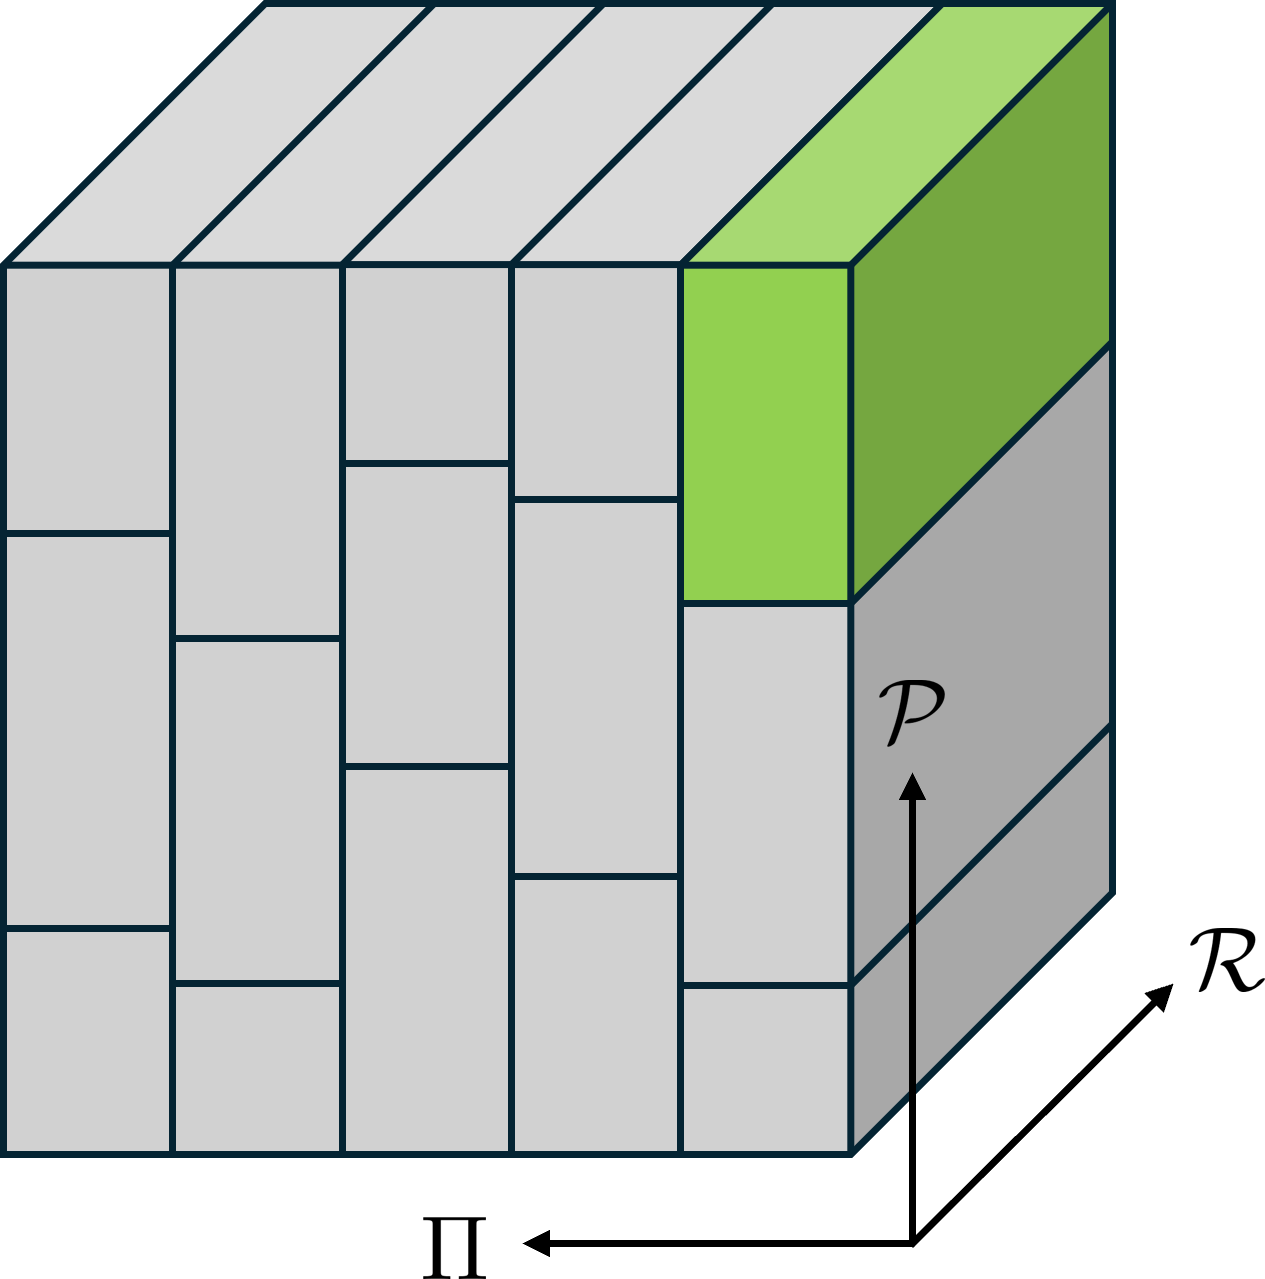
\includegraphics[width=0.3\textwidth]{Picture1.png}
\caption{Partitioning for hybrid MDPs}\label{fig: illustrate}
\end{figure}

\pref{fig: illustrate} illustrates the partition scheme over $\calM\times \Pi=\calP\times \calR\times \Pi$ described in \pref{assum: function approximation hybrid}. Each infoset $\phi$ (represented by the green block in \pref{fig: illustrate}) is associated with single policy $\pi_\phi$, a subset of transitions, and all reward functions. %Under a fixed policy $\pi$, transition $P$ and transition $P'$ should lie in the same $\phi$ if $Q^{\pi}(s,a; (P, R)) = Q^{\pi}(s,a; (P', R))$ for all $s,a,R$. 
As shown in \pref{fig: illustrate}, the partition over the $\calP$ space could be different for different $\pi$. 


\newpage
\section{Omitted Details in \pref{sec:pre}} \label{app: recovering}
In this section, we show that the algorithms in \cite{xu2023bayesian} and \cite{liu2025decision} are special cases of \pref{alg:general}. 

\subsection{Recovering \pref{thm: air phi}} The decision rule of \cite{liu2025decision}'s algorithm corresponds to \pref{eq:minmax} with $D^\pi(\nu\|\rho) = \E_{M\sim \nu}\E_{o\sim M(\cdot|\pi)}[\KL(\nu_{\bo{\phi}}(\cdot|\pi,o), \rho)]$. It can be shown that $\breg_{D^\pi(\cdot\|\rho)}(\nu, \nu')=\E_{M \sim \nu}\E_{o \sim M(\cdot|\pi)}\big[\KL(\nu_{\bo{\phi}}(\cdot|\pi, o), \nu'_{\bo{\phi}}(\cdot|\pi, o))\big]$ in this case. Furthermore, notice that when $\nu=\delta_{M_t, \picirc}$, we have $\nu_{\bo{\phi}}(\cdot|\pi, o)=\delta_{\phi^\star}$ according to \pref{def: restricted env}. Thus, the estimation error term in \pref{eq:minimax-guarantee} in \cite{liu2025decision}'s algorithm is 
\begin{align*}
    \E[\est] &= \E\left[\sum_{t=1}^T \left( \KL(\delta_{\phi^\star}, \rho_t) - \E_{o\sim M_t(\cdot|\pi_t)} \Big[\KL(\delta_{\phi^\star},  (\nu_t)_{\bo{\phi}}(\cdot|\pi_t,o))\Big]\right) \right] \\
    &= \E\left[\sum_{t=1}^T \left( \KL(\delta_{\phi^\star}, \rho_t) - \KL(\delta_{\phi^\star},  (\nu_t)_{\bo{\phi}}(\cdot|\pi_t,o_t))\right) \right] = \E\left[ \sum_{t=1}^T \log\frac{\nu_t(\phi^\star|\pi_t,o_t)}{\rho_t(\phi^\star)} \right],   
\end{align*}
where in the second equality we use that $o_t$ is drawn from $M_t(\cdot|\pi_t)$. 
%Specifically, if we choose $F_1(\pi, \nu, \rho_t) = \frac{1}{\eta}\E_{(M,\pi^\star) \sim \nu}\E_{z \sim M(\pi)}\left[\KL(\nu_{\bo{\phi}}(\cdot|\pi, z), \rho_t)\right]$ and $F_2(\rho; \pi_t, z_t) = \KL\left(\rho, \nu_{\bo{\phi}}(\cdot|\pi_t, z_t)\right)$, then the $\air^{\Phi}_{F_1, \rho_t}(p,\nu)$ is exactly the standard $\Phi$-AIR defined in \pref{eq:phiair}. Moreover, $\rho_{t+1} = \argmin_{\rho \in \Delta(\Phi)} F_2(\rho, \pi_t, z_t) = \nu_{\bo{\phi}}\left(\cdot|\pi_t, z_t\right)$. This exactly recovers the algorithm in \cite{liu2025decision}. Since the Bregman divergence $D_{F_1}(\nu, \nu') = \E_{(M,\pi^\star) \sim \nu}\E_{z \sim M(\pi)}\left[\KL\left(\nu_{\bo{\phi}}(\cdot|\pi, z), \nu'_{\bo{\phi}}(\cdot|\pi, z)\right)\right]$. Let $\phi_t^\star$ be the aggregation that $(M_t, \pi^\star)$ lies in,  the overhead in \pref{eq:minimax-guarantee} now becomes 
%\begin{align}
%    \frac{1}{\eta}\E_{\pi \sim p_t}\E_{o \sim M_t(\pi)}\left[\log\left(\frac{\nu_t(\phi^\star_t|\pi, z)}{\rho_t(\phi_t^\star)}\right)\right] =  \frac{1}{\eta}\E_{\pi \sim p_t}\E_{z \sim M_t(\pi)}\left[\log\left(\frac{\nu_t(\phi^\star_t|\pi, z)}{\nu_{t}(\phi_t^\star|\pi_t, z_t)}\right)\right] +  \frac{1}{\eta}\log\left(\frac{\rho_{t+1}(\phi_t^\star)}{\rho_t(\phi_t^\star)}\right) \label{eq:special-overhead}
%\end{align}
Thus, by letting $\rho_{t+1}(\phi) = \nu_t(\phi|\pi_t,o_t)$, their algorithm achieves $\E[\est] = \E\left[\sum_{t=1}^T \log\frac{\rho_{t+1}(\phi^\star)}{\rho_t(\phi^\star)} \right]\leq \log\frac{1}{\rho_1(\phi^\star)}=\log|\Phi|$. 
%For all the learnable instances discussed in \cite{xu2023bayesian} and \cite{liu2025decision}, $\phi_t^\star = \phi^\star$ for every $t \in [T]$ where $\phi^\star$ is a fixed aggregation. For instance, following the discussion on $\Phi$ in \pref{sec:pre},  model-based RL in stochastic settings has $M_t = M^\star$ and $\pi^\star = \pi_{M^\star}$, thus $\phi^\star = \phi_{M^\star}$, while model-free RL has  $\phi^\star = \phi_{Q^\star}$ where $Q^\star$ is the optimal $Q$ function of model $M^\star$.  For adversarial bandit, $M_t$ is changing over time but $\pi^\star$ is fixed, so $\phi^\star = \phi_{\pi^\star}$. For hybrid MDPs, transition $P^\star$ and comparator policy $\pi^\star$ are fixed over episodes so $\phi^\star = \phi^\star_{P^\star, \pi^\star}$. Given $\phi_t^\star = \phi^\star$, putting 
Using this in \pref{eq:minimax-guarantee} proves \pref{thm: air phi}. The results of \cite{xu2023bayesian} can also be recovered as they are special cases of \cite{liu2025decision}. 
%\begin{align*}
%    \E[\Reg] \le T \cdot \max_{\rho \in \Delta(\Phi)}\min_{p \in \Delta(\Pi)}\max_{\nu \in \Delta(\Psi)}\air^{\Phi}_{\rho, \eta}(p,\nu) + \frac{1}{\eta}\log(|\Phi|)
%\end{align*}
%which is exactly the regret bound derived in \cite{liu2025decision} and cover the results in \cite{xu2023bayesian}. The complexity measure based on $\Phi$-AIR is tightly related with DEC and uncover the learnability of numerous instances in stochastic, adversarial and hybrid settings. However, the $\Phi$-AIR approaches still fall short to deal with hybrid settings with full information feedback and model-free learning in either stochastic or hybrid settings. Our framework \pref{alg:general} can tackle both of these challenges with carefully designed $F_1$ and $F_2$.

\subsection{Recovering results for adversarial MDP with full-information feedback \citep{liu2025decision}}  
For learning with full information feedback in the adversarial MDPs, the learner can observe the full reward function at the end of each episode. In other words, at episode $t$, the reward function $R_t: \calS\times \calA\to [0,1]$ is part of the observation $o_t$. In this setting, the $\log|\Pi|$ dependence in the regret bound can be improved to $\log|\calA|$. To achieve this, \cite{liu2025decision} designed a two-level algorithm and define a new notion called InfoAIR. We can recover this result by instantiating our \pref{alg:general} with $\Phi=\{\phi_{P,(a_s)_{s\in\calS}}:~ P\in\calP, a_s \in\calA, \forall s\in\calS\}$ where $\phi_{P,(a_s)_{s\in\calS}} = \{((P, R), \pi^\star): R\in\calR, \pi^\star=(a_s)_{s\in\calS}\}$, that is, partitioning $\calM\times \Pi$ according to the transition kernel and the actions taken by the policy on all states.  
Then define 
\begin{align*}
   D^\pi(\nu\| \rho) = \E_{(P,R,\pi^\star) \sim \nu}\E_{o \sim M_{P,R}(\cdot|\pi)}\E_{s \sim d^{\pi, P}}\left[\KL(\nu_{\bo{a}_s, \bo{P}}(\cdot|\pi, o), \rho_{\bo{a}_s, \bo{P}})\right], 
\end{align*}
where $M_{P, R}$ denotes the MDP model with transition kernel $P$ and reward function $R$, and $\rho_{\bo{a}_s, \bo{P}}$ denotes $\rho$'s marginal distribution over $(a_s, P)$ following our notational convention. Finally, update the posterior as 
%where $\nu(a, P|\pi, o, s) = \sum_{\pi^\star \in \Pi}\pi^\star(a|s)\nu(\pi^\star, P|\pi, o, R, s)$, and  
$\rho_{t+1} = \argmin_{\rho}\sum_{s \in \calS}\KL\left(\rho_{\bo{a}_s, \bo{P}}, \nu_{\bo{a}_s, \bo{P}}(\cdot|\pi_t, o_t)\right)$. This recovers the same regret bound as in \cite{liu2025decision} without the need for the two-level design. %Such design of $F_1$ and $F_2$ take advantages of the full information structure by putting the whole reward function into the condition of $\nu$. This enables the belief $\nu$ can be updated in the action space $\calA$ at every state instead of the whole policy space $\Pi$, which is analog to policy optimization approaches \citep{sherman2023rate, liu2023towards, casselwarm}. 
We also note that the analysis for this result requires our new proof strategy in \pref{eq:general-decom}, as the $D^\pi(\nu\|\rho)$ here is not strictly convex in $\nu$ and the previous proof \cite{xu2023bayesian, liu2025decision} cannot be applied. %\cw{The notation in this paragraph is confusing ($\rho(\cdot|s)?$) and there is no definition of $\Phi$ here. }




%More importantly, for model-free learning, standard $\Phi$-AIR can only handle very restricted instance in stochastic settings and fails to be extended to hybrid settings. \cite{liu2025decision} design a separate algorithm based on optimistic DEC to handle model-free learning in hybrid settings with full information feedback. Their approach, however, cannot be extended to bandit feedback settings due to technical limitations. We will show that, with carefully chosen of $F_1, F_2$ in our framework \pref{alg:general}, we not only improve the standard optimistic DEC designed for model-free RL in stochastic settings (\pref{sec:stochastic}), but also, for the first time, provide an approach to deal with model-free learning in hybrid settings with general function approximation (\pref{sec:hybrid}).  



\newpage
\section{Concentration Inequality}
\begin{lemma}[Freedman's inequality \citep{beygelzimer2011contextual}]\label{lem: strengthen freed}
    Let $X_1, X_2,\ldots$ be a martingale difference sequence with respect to a filtration $\mathfrak{F}_1 \subset \mathfrak{F}_2 \subset \cdots$ such that $\E[X_t|\mathfrak{F}_t]=0$ and assume $X_t\leq B$ almost surely. Then for any $\alpha\geq B$, with probability at least $1-\delta$, 
    \begin{align*}
        \sum_{t=1}^T X_t \leq \frac{1}{\alpha} \sum_{t=1}^T \E[X_t^2|\mathfrak{F}_t] + \alpha \log (1/\delta).  \numberthis \label{eq: to substitutate}
    \end{align*}
    %where 
    % \begin{align*}
    %    V_T = \sum_{t=1}^T \E[X_t^2|\mathfrak{F}_t], \quad U_T =  \max\left\{\epsilon, \max_{t\in[T]} |X_t|\right\}. 
    %\end{align*}
\end{lemma}

\begin{lemma}[Empirical Freedman's inequality]\label{lem: empirical freed}
    Let $X_1, X_2,\ldots$ be a sequence with respect to a filtration $\mathfrak{F}_1 \subset \mathfrak{F}_2 \subset \cdots$ such that $\E[X_t|\mathfrak{F}_t]=\mu_t$ and assume $\max\{X_t-\mu_t,X_t\}\leq B$ almost surely. Then for any $\alpha\geq 4B$, with probability at least $1-\delta$, 
    \begin{align*}
        \sum_{t=1}^T (\mu_t - X_t) \leq \frac{4}{\alpha} \sum_{t=1}^T X_t^2 + \alpha \log (1/\delta).  \numberthis \label{eq: to empirical substitutate}
    \end{align*}
    %where 
    % \begin{align*}
    %    V_T = \sum_{t=1}^T \E[X_t^2|\mathfrak{F}_t], \quad U_T =  \max\left\{\epsilon, \max_{t\in[T]} |X_t|\right\}. 
    %\end{align*}
\end{lemma}
\begin{proof}
    Denote $\E_t[\cdot]=\E[\cdot~|~\mathfrak{F}_t]$. We have at any time step
    \begin{align*}
    &\E_{t}\left[\exp\left(\frac{1}{\alpha}(\mu_t - X_t) - \frac{4}{\alpha^2}X_t^2\right)\right]
    \\&\leq \E_{t}\left[1+ \frac{1}{\alpha}(\mu_t - X_t) - \frac{4}{\alpha^2}X_t^2 +\left(\frac{1}{\alpha}(\mu_t - X_t) - \frac{4}{\alpha^2}X_t^2\right)^2\right]
    \\&\leq 1+\E_{t}\left[ - \frac{4}{\alpha^2}X_t^2 +\frac{2}{\alpha^2}((\mu_t - X_t)^2+X_t^2)\right]\leq 1. 
    \end{align*}
    Markov inequality finishes the proof.
\end{proof}

\begin{lemma}\label{lem: useful inequali}
    Let $(X_1, Y_1), (X_2, Y_2)\ldots$ be a sequence with respect to a filtration $\mathfrak{F}_1 \subset \mathfrak{F}_2 \subset \cdots$ such that $|X_t|\leq B$ and $0\leq Y_t\leq B$ almost surely. Furthermore, $\E[X_t|\mathfrak{F}_t]\geq \E[Y_t|\mathfrak{F}_t] $ and $B\E[X_t|\mathfrak{F}_t]\geq \E[X_t^2|\mathfrak{F}_t]$. Then with probability at least $1-\delta$, 
    \begin{align}
        \frac{1}{2}\sum_{t=1}^T \E[X_t|\mathfrak{F}_t] \leq \sum_{t=1}^T \left(X_t - \frac{1}{4}Y_t\right) + 9B\log(1/\delta).\label{eq: useful 11}  
    \end{align}
    Also, with probability at least $1-\delta$, 
    \begin{align}
        \frac{1}{2}\sum_{t=1}^T X_t \leq \sum_{t=1}^T \left(X_t - \frac{1}{4}Y_t\right) + 9B\log(1/\delta).\label{eq: useful 22}   
    \end{align}
    
\end{lemma}
\begin{proof}
    Denote $\E_t[\cdot]=\E[\cdot~|~\mathfrak{F}_t]$. Let $c\in[\frac{1}{2},1]$ be a fixed constant, and define $Z_t = cX_t - \frac{1}{4}Y_t$. Applying \pref{lem: strengthen freed} with $\alpha=9B$ gives 
    \begin{align*}
        \sum_{t=1}^T  \left(\E_t[Z_t] - Z_t\right) 
        &\leq \frac{1}{9B}\sum_{t=1}^T  \E_t[(\E_t[Z_t] - Z_t)^2] + 9B\log(1/\delta) \\
        &\leq \frac{1}{9B}\sum_{t=1}^T  \E_t[Z_t^2] + 9B\log(1/\delta) \\
        &\leq \frac{1}{9B} \sum_{t=1}^T \left(2c^2\E_t[X_t^2] + \frac{2}{16}\E_t[Y_t^2] \right) + 9B\log(1/\delta) \\
        &\leq \frac{1}{9} \sum_{t=1}^T \left(2c^2\E_t[X_t] + \frac{2}{16}\E_t[X_t] \right) + 9\log(1/\delta) \tag{$\E_t[Y_t^2]\leq B\E_t[Y_t]$ because $Y_t\in[0,B]$}
    \end{align*}
    Rearranging:  
    \begin{align}
       \sum_{t=1}^T \E_t\left[Z_t - \left(\frac{2c^2}{9} + \frac{1}{72}\right)X_t\right]\leq \sum_{t=1}^T Z_t + 9B\log(1/\delta). \label{eq: useful44}
    \end{align}
    To prove \pref{eq: useful 11}, let $c=1$, which gives 
    $\E_t\left[Z_t - \left(\frac{2c^2}{9} + \frac{1}{72}\right)X_t\right]= \E_t\left[X_t - \frac{1}{4}Y_t - \frac{17}{72} X_t\right] \geq \frac{1}{2}\E_t[X_t]  $. Combining this with \pref{eq: useful44} proves \pref{eq: useful 11}. To prove \pref{eq: useful 22}, let $c=\frac{1}{2}$. which gives  $\E_t\left[Z_t - \left(\frac{2c^2}{9} + \frac{1}{72}\right)X_t\right]= \E_t\left[\frac{1}{2}X_t - \frac{1}{4}Y_t - \frac{5}{72} X_t\right] \geq 0$. Combining this with \pref{eq: useful44} and rearranging proves \pref{eq: useful 22}. 
\end{proof}

\newpage
\section{Mirror Descent}

\begin{lemma}[First-order optimality condition]\label{lem: bregman}
   For any concave and differentiable function $F$, if $\nu'\in\argmax_{\nu\in\Omega} F(\nu)$ for some convex set $\Omega$, then $F(\nu)\leq F(\nu') - \breg_{(-F)}(\nu, \nu')$ for any $\nu\in\Omega$. 
\end{lemma}
\begin{proof}
Define $G = -F$. Then $G$ is convex and $\nu'\in\argmin_{\nu'} G(\nu')$. We have by the definition of Bregman divergence $\breg_G(\nu, \nu')= G(\nu) - G(\nu') - \langle \nabla G(\nu'), \nu-\nu'\rangle$, and first-order optimality condition $\langle \nabla G(\nu'), \nu-\nu'\rangle \ge 0$. Thus, $G(\nu) \ge G(\nu') + \breg_G(\nu, \nu')$, which is equivalent to $F(\nu) \le F(\nu') + \breg_{(-F)}(\nu, \nu')$.
\end{proof}

\begin{lemma}\label{lem:stability}
    Let $g: \Phi\to [-1,1]$ be any function and let $\nu, \rho\in\Delta(\Phi)$. Then for any $\eta>0$, 
    \begin{align*}
        \E_{\phi\sim \nu}[g(\phi)] - \E_{\phi\sim \rho}[g(\phi)] - \frac{1}{\eta} \KL(\nu, \rho) \leq \eta. 
    \end{align*}
\end{lemma}
\begin{proof}
    \begin{align*}
        \E_{\phi\sim \nu}[g(\phi)] - \E_{\phi\sim \rho}[g(\phi)] \leq 2D_{\text{TV}}(\nu, \rho) \leq 2\sqrt{\KL(\nu, \rho)}\leq \frac{1}{\eta}\KL(\nu, \rho) + \eta, 
    \end{align*}
    where we use Pinsker's inequality and AM-GM inequality. 
\end{proof}


\begin{lemma}[Mirror descent with auxiliary terms]\label{lem: mirror descent}
Let $F_t$ be a convex function over $\Delta_N$, and let $\ell_t, b_t\in\mathbb{R}^N$ with $\ell_t^2$ denoting $(\ell_t(1)^2, \ldots, \ell_t(N)^2)$. Then the update $p_1=\frac{1}{N}\mathbf{1}$ and 
    \begin{align*}
        p_{t+1} = \argmin_{p\in\Delta_N} \Big\{ 
  \inner{p, \ell_t + 4\gamma \ell_t^2 + b_t} + F_t(p) + \frac{1}{\gamma}\KL(p, p_t)\Big\}
    \end{align*}
    with $\gamma |\ell_t(i)|\leq \frac{1}{16}$ and $0\leq \gamma b_t(i)\leq \frac{1}{4}$ for all $i\in[N]$  ensures for any $p^\star\in\Delta_N$, 
    \begin{align*}
       &\sum_{t=1}^T \inner{p_t,\ell_t} \\
       &\leq \frac{\log N}{\gamma} + \sum_{t=1}^T \Big(\inner{p^\star, \ell_t + 4\gamma\ell_t^2} + \inner{p^\star, b_t} - \frac{1}{2}\inner{p_t,b_t} + F_t(p^\star) - F_t(p_{t+1}) - \breg_{F_t}(p^\star, p_{t+1})\Big). 
    \end{align*}
    
\end{lemma}
\begin{proof}
    By \pref{lem: bregman}, 
    \begin{align*}
        &\inner{p_{t+1}, \ell_t + 4\gamma\ell_t^2 + b_t} + F_t(p_{t+1}) + \frac{1}{\gamma}\KL(p_{t+1}, p_t) \\
        &\leq \inner{p^\star, \ell_t + 4\gamma\ell_t^2 + b_t} + F_t(p^\star) + \frac{1}{\gamma}\KL(p^\star, p_t) - \breg_{F_t}(p^\star, p_{t+1}) - \frac{1}{\gamma}\KL(p^\star, p_{t+1}). 
    \end{align*}
    Rearranging gives 
    \begin{align*}
        &\inner{p_t, \ell_t + 4\gamma\ell_t^2} \\
        &\leq \inner{p^\star, \ell_t + 4\gamma \ell_t^2} +  \inner{p_t-p_{t+1}, \ell_t + 4\gamma\ell_t^2 + b_t} - \frac{1}{\gamma} \KL(p_{t+1}, p_t) \\
        &\quad  + \inner{p^\star - p_{t}, b_t} + \frac{\KL(p^\star, p_t) - \KL(p^\star, p_{t+1})}{\gamma} + F_t(p^\star) - F_t(p_{t+1}) - \breg_{F_t}(p^\star, p_{t+1}).   \label{eq: apply here}  \numberthis
    \end{align*}
    Since $\gamma |\ell_t(i) + 4\gamma\ell_t(i)^2 + b_t(i)|\leq \frac{1}{16} + 4\times (\frac{1}{16})^2 + \frac{1}{4}\leq 1$, by \pref{lem:stability} we have 
    \begin{align*}
        &\inner{p_t-p_{t+1}, \ell_t + 4\gamma\ell_t^2 + b_t} - \frac{1}{\gamma} \KL(p_{t+1}, p_t) \\
        &\leq \gamma\inner{p_t, (\ell_t + 4\gamma\ell_t^2 + b_t)^2} \\
        &\leq 2\gamma \inner{p_t, ({\textstyle \frac{5}{4}}\ell_t)^2} + 2\gamma\inner{p_t, b_t^2} \\
        &\leq \inner{p_t, 4\gamma\ell_t^2} + \frac{1}{2}\inner{p_t, b_t}. 
    \end{align*}
    Using this in \pref{eq: apply here} we get 
    \begin{align*}
        \inner{p_t, \ell_t} 
        &\leq \inner{p^\star, \ell_t + 4\gamma\ell_t^2} + \inner{p^\star, b_t} - \frac{1}{2}\inner{p_t, b_t} \\
        &\qquad + \frac{\KL(p^\star, p_t) - \KL(p^\star, p_{t+1})}{\gamma} + F_t(p^\star) - F_t(p_{t+1}) - \breg_{F_t}(p^\star, p_{t+1}). 
    \end{align*}
    Summing over $t$ gives the desired inequality. 
\end{proof}

\iffalse
\begin{lemma}[Strengthened Freedman's inequality \cite{zimmert2022return}]\label{lem: strengthen freed}
    Let $X_1, X_2,\ldots$ be a martingale difference sequence with respect to a filtration $\mathfrak{F}_1 \subset \mathfrak{F}_2 \subset \cdots$ such that $\E[X_t|\mathfrak{F}_t]=0$ and assume $|X_t|\leq \infty$ almost surely. Let $\epsilon > 0$ be a fixed number. Then with probability at least $1-\delta$, 
    \begin{align*}
        \sum_{t=1}^T X_t \leq 3\sqrt{V_T \log \frac{2\max\{U_T, \sqrt{V_T}\}}{\epsilon\delta}} + 2U_T \log \frac{2\max\{U_T, \sqrt{V_T}\}}{\epsilon\delta}\numberthis \label{eq: to substitutate}
    \end{align*}
    where 
     \begin{align*}
        V_T = \sum_{t=1}^T \E[X_t^2|\mathfrak{F}_t], \quad U_T =  \max\left\{\epsilon, \max_{t\in[T]} |X_t|\right\}. 
    \end{align*}
    
\end{lemma}



\begin{proof}
    This is a direct corollary of the Theorem~9 of \cite{zimmert2022return}. We apply their Theorem~9 with $X_t' = \frac{X_t}{\epsilon}$, which gives 
    \begin{align*}
        \sum_{t=1}^T X_t' \leq 3\sqrt{V_T' \log \frac{2\max\{U_T', \sqrt{V_T'}\}}{\delta}} + 2U_T' \log \frac{2\max\{U_T', \sqrt{V_T'}\}}{\delta}
    \end{align*}
    where 
    \begin{align*}
        V_T' = \sum_{t=1}^T \E[X_t'^2|\mathfrak{F}_t] = \frac{1}{\epsilon^2}V_T, \quad U_T' =  \max\left\{1, \max_{t\in[T]} |X_t'|\right\} = \frac{1}{\epsilon}U_T. 
    \end{align*}
    Substituting $(V_T', U_T')$ with $(V_T, U_T)$ in \pref{eq: to substitutate} gives the inequality. 
\end{proof}
\fi


%\section{Proof for Full-Information Feedback}
%\label{app:full-info-proof}

%\begin{theorem}
%\HL{This is a theorem for full-info}
%\label{thm:full-info}    
%\end{theorem}


\newpage
\section{Estimation Procedures}
We present the choices of \postupdate as standalone online learning algorithms because they might be of independent interest.



\subsection{Average estimation error minimization via batching}\label{app: batching improve}


\begin{algorithm}[H]
    \caption{Epoch-based learning algorithm for average estimation error}
    \label{alg:MF-Epoch-final}
    \textbf{Input}: An estimation function $\ell_h: \Phi\times \calO\to [-B, B]^N$ satisfying \pref{assum: avg err}. \\
    \textbf{Parameter:} $\tau = T^{\frac{1}{3}}, \beta = 7\tau N\iota$, $\gamma = \frac{1}{2\beta}$, $\iota = \log(12NKH/\delta)$. \\
    \For{$k=1, 2, \ldots, K$}{
         Receive observations $o_t\sim M_t(\cdot|\pi_k)$ for all 
         $t\in\calI_k = \{(k-1)\tau +1, \ldots, k\tau\}$. \\ Split $\calI_k$ into two sub-intervals of equal size: 
         \begin{align*}
             \calI_k^{\leftt} = \{(k-1)\tau +1, \ldots, (k-1)\tau +\tfrac{\tau}{2}\}  \quad \text{and} \quad \calI_k^{\rightt} = \{(k-1)\tau + \tfrac{\tau}{2} +1 , \ldots, k\tau\}. 
         \end{align*}
         %For all $h,\phi$ and all $t\in\calI_k$, receive $\ellest_h(\phi; o_{t,h}) \in[-B,B]^N$.\\ % of conditionally independent random variables with mean $\bar\ell_{k,h}(\phi)\in [-B,B]^N$. \\
         Define for all $j\in[N]$,  
         \begin{align*}
             %&\Delta_t(\phi',\phi) = \frac{1}{H}\sum_{h=1}^H \left(f_{\phi'}(s_{t,h}, a_{t,h}) - r_{t,h} - f_\phi(s_{t,h+1})\right)^2, \\
             L_k(\phi)_j &=\frac{\tau}{B^2 H}\sum_{h=1}^H \left(\frac{1}{|\calI_k^\leftt|}\sum_{t\in\calI_k^\leftt} \ell_{h}(\phi; o_{t,h})_j\right)\left(\frac{1}{|\calI_k^\rightt|}\sum_{t\in\calI_k^\rightt} \ell_h(\phi; o_{t,h})_j\right)\,,\quad L_k(\phi) = \sum_{j=1}^N L_k(\phi)_{j}. 
         \end{align*}
         
         
         Let $(F_t)_{t\in\calI_k}: \Delta(\Phi)\to \mathbb{R}$ be convex functions. Calculate % for $L_k(\phi)=L_{k}(\phi)_{j^k_\phi}$
        \begin{align*}
             &\rho_{k+1} = \argmin_{\rho\in \Delta(\Phi)}\left\{\inner{\rho,  L_k + (4\gamma+2\beta^{-1}) L_k^2} + \sum_{t\in\calI_k}F_t(\rho) + \frac{1}{\gamma}\KL(\rho, \rho_k) \right\}.   \label{eq: epoch level update} \numberthis   
        \end{align*}
    }
\end{algorithm}
\begin{lemma}\label{lem: est part1}
With probability at least $1-\delta/3$,  
\pref{alg:MF-Epoch-final} satisfies
\begin{align*}
    \frac{1}{B^2H}\sum_{k=1}^K \sum_\phi \rho_k(\phi) \sum_{t\in\calI_k} \max_{j\in[N]} \sum_{h=1}^H \left(\E^{\pi_k, M_t}[\ell_h(\phi; o_{h})_j]  \right)^2 \leq \sum_{k=1}^K\sum_{\phi}\rho_{k}(\phi)\left(L_k(\phi) + \frac{1}{\beta}L_k(\phi)^2\right)+4\beta\log(3/\delta)\,.
\end{align*}
\end{lemma}
\begin{proof}
By \pref{assum: avg err}, for any $t,t'\in\calI_k$ it holds that
\begin{align*}
    \E^{\pi_k, M_t}\left[ \ell_h(\phi; o_{h}) \right] = \E^{\pi_k, M_{t'}}\left[ \ell_h(\phi; o_{h}) \right]. 
\end{align*}
We denote $\bar\ell_{k,h}(\phi) = \E^{\pi_k, M_t}[\ell_h(\phi; o_{h})]$ for any $t\in\calI_k$. 

Clearly, the left-hand side of the desired inequality is upper bounded by  
\begin{align*}
    \frac{1}{B^2H}\sum_{k=1}^K \sum_\phi \rho_k(\phi) \sum_{t\in\calI_k} \sum_{j=1}^N \sum_{h=1}^H \left(\E^{\pi_k, M_t}[\ell_h(\phi; o_{h})_j]  \right)^2 = \frac{\tau}{B^2H} \sum_{k=1}^K\sum_{\phi}\rho_{k}(\phi)\sum_{j=1}^N \sum_{h=1}^H\bar\ell_{k,h}(\phi)^2_j 
\end{align*}
By construction, $\E_{k}[L_k(\phi)]=\frac{\tau}{B^2H}\sum_{j=1 }^N\sum_{h=1}^H\bar\ell_{k,h}(\phi)^2_j$ due to the conditional independence of the observations. Furthermore, we have $L_k(\phi)\in[-\tau N,\tau N]$. Therefore, we can use \pref{lem: empirical freed} on the sequence $X_k=-\sum_{\phi}\rho_k(\phi)L_k(\phi)$ with $\beta \geq 7\tau N$: 
    \begin{align*}
        \frac{\tau}{B^2H}\sum_{k=1}^K\sum_{\phi}\rho_{k}(\phi)\sum_{j=1}^N\sum_{h=1}^H\bar\ell_{k,h}(\phi)^2_j\leq\sum_{k=1}^K\sum_{\phi}\rho_{k}(\phi)\left(L_k(\phi) + \frac{1}{\beta}L_k(\phi)^2\right)+4\beta\log(3/\delta)\,.
    \end{align*}
\end{proof}
\begin{lemma}\label{lem: est part2}
    With probability at least $1-\delta/3$,
    \begin{align*}
        \sum_{k=1}^KL_k(\phi^\star)^2 \leq KN^2\log^2(12NKH/\delta). 
    \end{align*}
\end{lemma}
\begin{proof}
By \pref{assum: avg err} and \pref{lem: strengthen freed}, for any $j,k,h$, we have with probability $1-\delta$, 
\begin{align*}
&\left|\sum_{t\in\calI_k^\leftt} \ell_{h}(\phi^\star, o_{t,h})_j\right| = \left|\sum_{t\in\calI_k^\leftt} \ell_{h}(\phi^\star, o_{t,h})_j - \sum_{t\in\calI_k^\leftt} \E^{\pi_k, M_t}[\ell_h(\phi^\star; o_h)] \right| \leq B\sqrt{\tau \log(12/\delta)}\\
&\left|\sum_{t\in\calI_k^\rightt} \ell_{h}(\phi^\star, o_{t,h})_j\right| = \left|\sum_{t\in\calI_k^\rightt} \ell_{h}(\phi^\star, o_{t,h})_j - \sum_{t\in\calI_k^\rightt} \E^{\pi_k, M_t}[\ell_h(\phi^\star; o_h)] \right| \leq B\sqrt{\tau \log(12/\delta)}\,.
\end{align*}
Via a union bound over all these events, this holds simultaneously for all $j,k,h$. Hence with probability $1-\delta$, we have $|L_k(\phi^\star)_j|\leq \frac{\tau}{B^2H} H\left(\frac{1}{\tau}B\sqrt{\tau \log(12NKH/\delta)}\right)^2=\log(12NKH/\delta) $ for all $j,k$ simultaneously.
Summing over $j$ and $k$ finishes the proof.
\end{proof}
\begin{lemma}\label{lem: est part3}
    With probability at least $1-\delta/3$, we have
    \begin{align*}
        \sum_{k=1}^KL_k(\phi^\star) \leq 
            \frac{1}{\beta}\sum_{k=1}^KL_k(\phi^\star)^2+4\beta \log(6/\delta)
    \end{align*}
\end{lemma}
\begin{proof}
    Define the random variable $X_k = \min\{L_k(\phi^\star),N\log(12NKH/\delta) \}$. 
    By \pref{lem: empirical freed} we have with probability at least $1-\delta/6$, 
    \begin{align*}
        \sum_{k=1}^KX_t \leq \frac{1}{\beta}\sum_{k=1}^KL_k(\phi^\star)^2 + 4\beta\log(6/\delta)\,, 
    \end{align*}
    where we use that $\E_k[X_k]\leq \E_k[L_k(\phi^\star)]=0$.
    Finally note that with probability $1-\delta/6$ we have $L_k(\phi^\star)=X_k$ for all $k$ by the proof of \pref{lem: est part2}. Combining both events finishes the proof.
\end{proof}
\begin{lemma}\label{lem: online esitmation epoch general}
    With probability at least $1-\delta$, \pref{alg:MF-Epoch-final} satisfies
    \begin{align*}
        &\frac{1}{B^2H}\sum_{k=1}^K\sum_{\phi}\rho_{k}(\phi)\sum_{t\in\calI_k}\max_{j\in[N]}\sum_{h=1}^H \left(\E^{\pi_k, M_t}\left[\ell_h(\phi;o_{h})_j\right]\right)^2 \le O\left(NT^{\frac{1}{3}}\log|\Phi|\right) \\
        &\quad +  \sum_{k=1}^K \sum_{t\in\calI_k}(  F_t(\delta_{\phi^\star}) - F_t(\rho_{k+1}) - \breg_{F_t}(\delta_{\phi^\star}, \rho_{k+1})).  
    \end{align*}
\end{lemma}

\begin{proof}[Proof of \pref{lem: online esitmation epoch general}]
By union bound, the events of \pref{lem: est part1}, \pref{lem: est part2}, and \pref{lem: est part3} hold simultaneously with probability $1-\delta$.
Observe that the update of $\rho_k$ (\pref{eq: epoch level update}) is in the form specified in \pref{lem: mirror descent}. 
Invoking \pref{lem: mirror descent} with $b_k=\frac{2}{\beta}L_k^2$, we get 
\begin{align*}
    &\sum_{k=1}^K  \inner{\rho_k, L_k+\frac{1}{\beta}L_k^2} 
    \leq \frac{\log|\Phi|}{\gamma} \numberthis \label{eq: miror descent bound 33}\\
    &\quad + \sum_{k=1}^K \left(L_k(\phi^\star) + \left(4\gamma+\frac{2}{\beta}\right) L_k(\phi^\star)^2 +\sum_{t\in\calI_k}(F_t(\delta_{\phi^\star}) - F_t(\rho_{k+1}) - \breg_{F_t}(\delta_{\phi^\star}, \rho_{k+1})) \right). \\
\end{align*}
    Chaining \pref{lem: est part2} and \pref{lem: est part3},  
    \begin{align*}
        &\sum_{k=1}^K \left(L_k(\phi^\star) + \left(4\gamma+\frac{2}{\beta}\right) L_k(\phi^\star)^2\right)
        \\ &\leq 4\beta\log(6/\delta)+\left(4\gamma + \frac{3}{\beta}\right)KN^2\log^2(12NKH/\delta). 
    \end{align*}
Using \pref{lem: est part1} and substituting $\beta = 7\tau N\iota$, $\gamma =\frac{1}{2\beta}$ yields
\begin{align*}
     \frac{1}{B^2H}\sum_{k=1}^K \sum_\phi \rho_k(\phi) \sum_{t\in\calI_k} \max_{j\in[N]} \sum_{h=1}^H \left(\E^{\pi_k, M_t}[\ell_h(\phi; o_{h})_j]  \right)^2 \leq 35 \tau N\iota + 20\frac{K N\iota}{\tau}
\end{align*}
Using $K=T/\tau$ and tuning $\tau = T^\frac{1}{3}$ yields $O(T^\frac{1}{3}N\iota)$.
\end{proof}


\subsection{Squared estimation error minimization via bi-level learning}\label{app: bilevel}
%In this section, we consider a general \emph{bi-level learning problem} and design a general algorithm to handle it. It will be used as a subroutine in algorithms for decouplable MDPs with Bellman completeness that achieves $\sqrt{T}$ regret.  



%\begin{assumption}\label{assum: bilevel}
%    Assume $\Delta_t: \Phi\times\Phi\to [0,B]$, and assume that for each $\phi\in\Phi$, there exists $\calT\phi\in\Phi$ such that for any $\phi'\in\Phi$, 
%    \begin{align*}
        %\E_t\left[\left(\Delta_t(\phi', \phi) - \Delta_t(\calT\phi, \phi)\right)^2\right]  \leq B\E_t\left[\Delta_t(\phi', \phi) - \Delta_t(\calT\phi, \phi)\right].    
    %\end{align*}
    %Also, assume there exists $\phi^\star\in\calR$ such that $\phi^\star=\calT\phi^\star$. 
%\end{assumption}
        
%The goal of the bi-level problem is to sequentially generate $\rho_t\in \Delta(\Phi)$ such that 
%\begin{align}
%    \sum_{t=1}^T \E_{\phi\sim \rho_t} \left[\Delta_t(\phi, \phi) - \Delta_t(\calT\phi, \phi)\right] = o(T). \label{eq: goal of bilevel}
%\end{align}
%According to \pref{assum: bilevel}, as long the learner can identify $\phi^\star$ and make $\rho_t$ concentrate on $\phi^\star$ then \pref{eq: goal of bilevel} can be achieved because $\Delta_t(\phi^\star, \phi^\star) - \Delta_t(\calT\phi^\star, \phi^\star) = \Delta_t(\phi^\star, \phi^\star) - \Delta_t(\phi^\star, \phi^\star)=0$. The challenge lies in that neither the identity of $\phi^\star$ nor the identity of $\calT\phi$ for each $\phi$ are known by the learner. 


\begin{algorithm}[H]
    \caption{Bi-level learning algorithm for squared estimation error}
    \label{alg:MF-BiLevel-final}
    \textbf{Input:} An estimation function $\err_h: \Phi\times\Phi\times \calO\to [0, B^2]$ satisfying \pref{assum: squared est err}. \\
    \textbf{Parameter:} $\iota = 64\log|\Phi|$, $\gamma=\frac{1}{4\iota}$. \\
   $\rho_1(\phi) = 1/|\Phi|,\, \forall \phi \in \Phi$ and  $q_1(\phi'|\phi) = 1/|\Phi|$, $\forall \phi', \phi\in \Phi$. \\
    \For{$t=1, 2, \ldots, T$}{
         Receive observation $o_t\sim M_t(\cdot|\pi_t)$. \\
         Define 
         \begin{align*}
             \Delta_t(\phi', \phi) &= \frac{1}{B^2H}\sum_{h=1}^H \err_h(\phi', \phi, o_{t,h}), \\
             %&\Delta_t(\phi',\phi) = \frac{1}{H}\sum_{h=1}^H \left(f_{\phi'}(s_{t,h}, a_{t,h}) - r_{t,h} - f_\phi(s_{t,h+1})\right)^2, \\
             L_t(\phi) &= \Delta_t(\phi, \phi) - \E_{\phi'\sim q_t(\cdot|\phi)}\left[\Delta_t(\phi', \phi)\right], 
             \\ 
             b_t(\phi) &= \frac{[\rho_t(\phi) - \max_{s<t}\rho_s(\phi)]_+}{\rho_t(\phi)} \iota. 
         \end{align*}
         Let $F_t: \Delta(\Phi)\to \mathbb{R}$ be a convex function. Calculate
        \begin{align*}
             &\rho_{t+1} = \argmin_{\rho\in \Delta(\Phi)}\left\{\inner{\rho,  L_t + 4\gamma L_t^2 +  b_t} + F_t(\rho) + \frac{1}{\gamma}\KL(\rho, \rho_t) \right\},  \label{eq: top level update} \numberthis \\
              & q_{t+1}(\phi'|\phi) \propto \exp\left(- \alpha_{t}(\phi) \sum_{s=1}^t \rho_s(\phi)\Delta_s(\phi',\phi)\right) \quad \text{where \ \ }  \alpha_{t}(\phi) = \frac{1}{16 \max_{s \le t} \rho_s(\phi)}.  
        \end{align*}
    }
\end{algorithm}


\begin{lemma}\label{lem: online esitmation bilinear outer general}
    With probability at least $1-\delta$, 
    \begin{align*}
        &\sum_{t=1}^T \inner{\rho_{t}, L_t} \le \frac{\log|\Phi|}{\gamma} \\
        &\quad +  \sum_{t=1}^T \left(- \frac{1}{2} \inner{\rho_{t}, b_t} + b_t(\phi^\star) +  F_t(\delta_{\phi^\star}) - F_t(\rho_{t+1}) - \breg_{F_t}(\delta_{\phi^\star}, \rho_{t+1}) \right) + O\left(\log(1/\delta)\right).  
    \end{align*}
\end{lemma}

\begin{proof}[Proof of \pref{lem: online esitmation bilinear outer general}]
Observe that the update of $\rho_t$ (\pref{eq: top level update}) is in the form specified in \pref{lem: mirror descent}. 
Invoking \pref{lem: mirror descent}, we get 
\begin{align*}
    &\sum_{t=1}^T  \inner{\rho_t, L_t} 
    \leq \frac{\log|\Phi|}{\gamma} \numberthis \label{eq: miror descnet bound 33}\\
    &\quad + \sum_{t=1}^T \left(L_t(\phi^\star) + 4\gamma L_t(\phi^\star)^2 +  b_t(\phi^\star)-\frac{1}{2}\inner{\rho_{t}, b_t}+F_t(\delta_{\phi^\star}) - F_t(\rho_{t+1}) - \breg_{F_t}(\delta_{\phi^\star}, \rho_{t+1}) \right). \\
\end{align*}
By \pref{assum: squared est err} we have %$\E_t[L_t(\phi^\star)]\leq 0$ 
%and 
\begin{align*}
    0\leq \E_t[L_t(\phi^\star)^2] 
    &= \E_t\left[\left(\Delta_t(\phi^\star, \phi^\star) - \E_{\phi'\sim q_t(\cdot|\phi^\star)}\left[\Delta_t(\phi', \phi^\star)\right]\right)^2\right] \\
    &\leq \E_{\phi'\sim q_t(\cdot|\phi^\star)}\left[\E_t\left[\left(\Delta_t(\phi^\star, \phi^\star) - \Delta_t(\phi', \phi^\star)\right)^2\right] \right] \tag{Jensen's inequality} \\
    &\leq \E_{\phi'\sim q_t(\cdot|\phi^\star)}\left[\E_t\left[\left(\Delta_t(\calT_{M_t}\phi^\star, \phi^\star) - \Delta_t(\phi', \phi^\star)\right)^2\right] \right] \tag{$M_t\in\phi^\star$ and thus $\calT_{M_t}\phi^\star=\phi^\star$} \\
    &\leq 4\E_{\phi'\sim q_t(\cdot|\phi^\star)}\left[\E_t\left[\Delta_t(\phi', \phi^\star) - \Delta_t(\calT_{M_t}\phi^\star, \phi^\star) \right] \right]  \tag{by \pref{assum: squared est err}} \\
    &= 4\E_{\phi'\sim q_t(\cdot|\phi^\star)}\left[\E_t\left[\Delta_t(\phi', \phi^\star) - \Delta_t(\phi^\star, \phi^\star) \right] \right] \\
    &= - 4\E_t[L_t(\phi^\star)]. 
\end{align*}
This allows us to apply \pref{lem: useful inequali} with $X_t = -L_t(\phi^\star)$ and $Y_t=\frac{1}{4}X_t^2$, which gives
\begin{align*}
    \sum_{t=1}^T \left(L_t(\phi^\star) + 4\gamma L_t(\phi^\star)^2\right) 
    &\leq \sum_{t=1}^T \left(L_t(\phi^\star) + \frac{1}{16} L_t(\phi^\star)^2\right) \\
    &\leq \frac{1}{2}\sum_{t=1}^T \E_t[L_t(\phi^\star)] + 36 \log(1/\delta)\leq 36\log(1/\delta).  
\end{align*}
Combining this with \pref{eq: miror descnet bound 33} finishes the proof. 
\end{proof}

\begin{lemma}\label{lem: max rho lemma 33}
    With probability at least $1-\delta$, 
    \begin{align*}
        \sum_{t=1}^T \E_{\phi\sim \rho_t} \E_{\phi'\sim q_t(\cdot|\phi)}[\Delta_t(\phi', \phi) - \Delta_t(\calT_{M_t}\phi, \phi)] \leq 32 \sum_\phi \max_{t\leq T} \rho_t(\phi) \log|\Phi| + 72\log(1/\delta). 
    \end{align*}
\end{lemma}
\begin{proof}
By \pref{assum: squared est err}, we have $\calT_{M_t}\phi = \calT_{M_{t'}}\phi$ for all $\phi$ and all $t,t'\in[T]$. We denote $\calT \phi = \calT_{M_{t}}\phi$ for any $t$. 
By the exponential weight update, for any $\phi$, 
\begin{align*}
    &\sum_{t=1}^T \sum_{\phi'} q_t(\phi'|\phi)\rho_t(\phi)\left(\Delta_t(\phi', \phi) - \Delta_t(\calT_{M_t}\phi, \phi)\right) 
 \\
 &= \sum_{t=1}^T \sum_{\phi'} q_t(\phi'|\phi)\rho_t(\phi)\left(\Delta_t(\phi', \phi) - \Delta_t(\calT\phi, \phi)\right) \\ 
    &\leq \frac{\log |\Phi|}{\alpha_T(\phi)} + \sum_{t=1}^T \sum_{\phi'}\alpha_t(\phi)q_t(\phi'|\phi)\rho_t(\phi)^2  \left(\Delta_t(\phi', \phi) - \Delta_t(\calT\phi, \phi)\right)^2 \\
    &\leq 16\max_{t\leq T}\rho_t(\phi) \log |\Phi| + \frac{1}{16}\sum_{t=1}^T \sum_{\phi'}q_t(\phi'|\phi)\rho_t(\phi)  \left(\Delta_t(\phi', \phi) - \Delta_t(\calT\phi, \phi)\right)^2.  
\end{align*}
Rearranging and summing over $\phi$:  
\begin{align*}
   &\sum_{t=1}^T \E_{\phi\sim \rho_t} \E_{\phi'\sim q_t(\cdot|\phi)}\left[\Delta_t(\phi', \phi) - \Delta_t(\calT\phi, \phi) - \frac{1}{16}(\Delta_t(\phi', \phi) - \Delta_t(\calT\phi, \phi))^2\right] \\
   &\qquad \qquad \leq 16 \sum_\phi \max_{t\leq T} \rho_t(\phi) \log|\Phi|.   \numberthis \label{eq: some bound 34}
\end{align*}
Define
\begin{align*}
    X_t &= \E_{\phi\sim \rho_t} \E_{\phi'\sim q_t(\cdot|\phi)}\left[\Delta_t(\phi', \phi) - \Delta_t(\calT\phi, \phi)\right], \\
    Y_t &= \frac{1}{4}\E_{\phi\sim \rho_t} \E_{\phi'\sim q_t(\cdot|\phi)}\left[\left(\Delta_t(\phi', \phi) - \Delta_t(\calT\phi, \phi)\right)^2\right].
\end{align*}
By \pref{assum: squared est err} we have $\E_t[Y_t]\leq \E_t[X_t]$. By Jensen's inequality, $\E_t[X_t^2]\leq 4B^2 H\E_t[Y_t]\leq 4B^2 H\E_t[X_t]$. Invoking \pref{lem: useful inequali} and using \pref{eq: some bound 34} give
\begin{align*}
    \frac{1}{2}\sum_{t=1}^T X_t &\leq \sum_{t=1}^T \left(X_t - \frac{1}{4}Y_t\right) + 36\log(1/\delta) 
    \leq 16 \sum_\phi \max_{t\leq T} \rho_t(\phi) \log|\Phi| + 36\log(1/\delta),  
\end{align*}
proving the desired inequality. 

\end{proof}

\begin{lemma}\label{lem: bilievel final bound}
   With probability at least $1-\delta$, 
  \begin{align*}
    &\sum_{t=1}^T \E_{\phi\sim \rho_t} \left[\Delta_t(\phi, \phi) - \Delta_t(\calT_{M_t}\phi, \phi)\right] \\
    &\leq \sum_{t=1}^T  \left(F_t(\delta_{\phi^\star}) - F_t(\rho_{t+1}) - \breg_{F_t}(\delta_{\phi^\star}, \rho_{t+1})\right) + O\left(\log^2(|\Phi|/\delta)\right). 
\end{align*}
\end{lemma}
\begin{proof}
By \pref{assum: squared est err}, we have $\calT_{M_t}\phi = \calT_{M_{t'}}\phi$ for all $\phi$ and all $t,t'\in[T]$. We denote $\calT \phi = \calT_{M_{t}}\phi$ for any $t$. 


\begin{align*}
    \E_{\phi\sim \rho_t}[L_t(\phi)] 
    &= \E_{\phi\sim \rho_t}[\Delta_t(\phi, \phi) - \E_{\phi'\sim q_t(\cdot|\phi)}[\Delta_t(\phi', \phi)]] \\
    &= \E_{\phi\sim \rho_t}\left[\Delta_t(\phi, \phi) - \Delta_t(\calT\phi, \phi) - \left(\E_{\phi'\sim q_t(\cdot|\phi)}[\Delta_t(\phi', \phi)] - \Delta_t(\calT\phi, \phi)\right)\right].
\end{align*}
Combining this with \pref{lem: online esitmation bilinear outer general}, we get 
\begin{align*}
   &\sum_{t=1}^T \E_{\phi\sim \rho_t} \left[\Delta_t(\phi, \phi) - \Delta_t(\calT\phi, \phi)\right] \\
   &\leq \frac{\log|\Phi|}{\gamma} + \sum_{t=1}^T \left(- \frac{1}{2} \inner{\rho_{t}, b_t} + b_t(\phi^\star) +  F_t(\delta_{\phi^\star}) - F_t(\rho_{t+1}) - \breg_{F_t}(\delta_{\phi^\star}, \rho_{t+1}) \right) \\
   &\qquad + O\left(\log(1/\delta)\right)   + \sum_{t=1}^T \E_{\phi\sim \rho_t}\E_{\phi'\sim q_t(\cdot|\phi)}\left[\Delta_t(\phi', \phi) - \Delta_t(\calT\phi, \phi)\right] \\
   &\leq \sum_{t=1}^T \left(- \frac{1}{2} \inner{\rho_{t}, b_t} + b_t(\phi^\star) +  F_t(\delta_{\phi^\star}) - F_t(\rho_{t+1}) - \breg_{F_t}(\delta_{\phi^\star}, \rho_{t+1})\right) \\
   &\qquad + O\left(\log^2(|\Phi|/\delta)\right)  + 32\sum_\phi \max_{t\leq T} \rho_t(\phi) \log|\Phi|.   \tag{by \pref{lem: max rho lemma 33} and the value of $\gamma$} %\\
   %& \numberthis \label{eq: blug 33}
\end{align*}

Note that 
\begin{align*}
    32\log|\Phi|\sum_{\phi}\max_{t \le T} \rho_{t}(\phi)  
    &= 32\log|\Phi|  \sum_{\phi}\left(\rho_1(\phi) +\sum_{t=2}^T [\rho_t(\phi)-\max_{s<t}\rho_s(\phi)]_+\right)
    \\&= 32\log|\Phi|   \sum_{\phi}\left(\rho_1(\phi) +\sum_{t=2}^T \rho_t(\phi)\frac{[\rho_t(\phi)-\max_{s<t}\rho_s(\phi)]_+}{\rho_t(\phi)}\right)
    \\&= \frac{1}{2} \sum_{t=1}^T \inner{\rho_t, b_t}  
\end{align*}
and 
\begin{align*}
    \sum_{t=1}^T b_t(\phi^\star) 
    &= O(\log|\Phi|)\times \sum_{t=1}^T \frac{\max_{s\leq t}\rho_s(\phi^\star) - \max_{s\leq t-1}\rho_s(\phi^\star)}{\max_{s\leq t}\rho_s(\phi^\star)} \\
    &\leq O(\log|\Phi|)\times \left(1+\sum_{t=2}^T  \ln \frac{\max_{s\leq t}\rho_s(\phi^\star)}{\max_{s\leq t-1} \rho_s(\phi^\star)}\right) \tag{$1-x\leq \ln \frac{1}{x}$}\\
    &\leq O\left(\log^2|\Phi|\right). 
\end{align*}
Combining inequalities above proves the lemma. 

\end{proof}




%which implies 
%\begin{align*}
%    \sum_{t=1}^T \sum_{\phi'} q_t(\phi'|\phi)\rho_t(\phi)\left(\Delta_t(\phi', \phi) - \Delta_t(\calT\phi, \phi)\right) \leq 43\max_{t\leq T}\rho_t(\phi) \log\left(\frac{4T|\Phi|^2}{\delta}\right) + \frac{3}{|\Phi|}\log\left(\frac{4T|\Phi|^2}{\delta}\right). 
%\end{align*}

\newpage
\section{Omitted Details in \pref{sec: general framework}}
\label{app:model-free stoc}
We define a batched version of \pref{alg:general} in \pref{alg:general batched}. When the batch size $\tau=1$, it is exactly \pref{alg:general}. One can also think of \pref{alg:general batched} as a special case of \pref{alg:general} where $\postupdate$ makes a real update only when $t=k\tau$ for $k=1,2,\ldots$, and keeps $\rho_{t+1}=\rho_t$ otherwise. 

\begin{algorithm}[H]
    \caption{General Batched Framework}
     \label{alg:general batched}
    \textbf{Input:} Partition set $\Phi$ and its union $\Psi$ (defined in \pref{sec: hybrid setting}). Batch size $\tau$. \\
    $\rho_1(\phi) = 1/|\Phi|,\, \forall \phi \in \Phi$. \\
    \For{$k=1, 2, \ldots, K$}{
       Set $p_k, \nu_k$ as the solution of the following minimax optimization (defined in \pref{eq: new AIR}): 
        \begin{align}
            \min_{p \in \Delta(\Pi)}\max_{\nu \in \Delta(\Psi)} \air^{\Phi, D}_\eta(p,\nu; \rho_k). 
            \label{eq:minmax batch}
        \end{align}
        Execute $\pi_k$ in rounds $t\in \{(k-1)\tau+1, \ldots, k\tau\}=\calI_k$ and receive observations $(o_t)_{t\in\calI_k}$. 
        \vspace{-5pt}
        \begin{flalign}
        &\text{Update\ } \rho_{k+1}= \postupdate(\nu_k, \rho_k, \pi_k, (o_t)_{t\in \calI_k}). && \label{eq:rho batch}
        \end{flalign}
        
        }
        \vspace{-3pt}
\end{algorithm}
\subsection{Assumption reductions}
\begin{proof}[Proof of \pref{lem: av assum reduction}]
In the stochastic setting, by \pref{assum: function approximation stochastic} we have $f_{\phi}(s,a)=Q^{\star}(s,a;M)$ and $f_{\phi}(s)=V^{\star}(s;M)$ for any $M\in\phi$. Hence
\begin{align*}
        \E^{\pi, M}[\ellest_h(\phi; o_h)] &= \E^{\pi, M}[f_{\phi}(s_h,a_h)-r_h-f_{\phi}(s_{h+1})]\\
        &=\E^{\pi, M}[Q^{\star}(s_h,a_h;M)-r_h-V^\star(s_{h+1};M)]=0.    
    \end{align*}
In the hybrid setting, we have by \pref{assum: function approximation hybrid} and \pref{assum: unique mapping} that 
$f_{\phi}(s,a;R)=Q^{\pi_{\phi}}(s,a;(P,R))$ and $f_{\phi}(s;R)=V^{\pi_{\phi}}(s;(P,R))$ for any $P\in\phi$. Hence, for any $j\in[d]$, defining $R'$ such that $R'(s,a)=\varphi(s,a)_j$, we have for $(P,R)\in\phi$, 
\begin{align*}
    \E^{\pi, (P,R)}[\ellest_h(\phi; o_h)_j] &= \E^{\pi, P}[f_{\phi}(s_h,a_h;R')-R'(s_h,a_h)-f_{\phi}(s_{h+1};R')]\\
        &=\E^{\pi, P}[Q^{\pi_{\phi}}(s_h,a_h;(P,R'))-R'(s,a)-V^{\pi_{\phi}}(s_{h+1};(P,R'))]=0. 
\end{align*}
Finally, note that in the stochastic setting $M_t=M^\star$, and in the hybrid setting $P_t=P^\star$, so the additional assumption always holds.
\end{proof}
\begin{proof}[Proof of \pref{lem: sq assum reduction}] 


In the stochastic setting, %this is a vector of dimension 1. %We further use $R_h$ to denote $r_h$ in the stochastic setting or the vector $\varphi(s_h,a_h)$ in the hybrid setting.
with \pref{assum: function approximation stochastic} and the Bellman completeness assumption (\pref{def: sto bc}), for any $M=(P,R)$, we define $\calT_M \phi\in\Phi$ as the $\phi'$ such that 
\begin{align*}
f_{\phi'}(s,a) = R(s,a) + \E_{s'\sim P(\cdot|s,a)}[f_\phi(s')]. 
%E_{(r_{h},s_{h+1})\sim M(s,a)}[R_h+f_{\phi}(s_{h+1})]=f_{\calT_M\phi}(s_h,a_h)\,.
\end{align*}
By \pref{def: sto bc}, such $\phi'$ always exists. 

In the hybrid setting, with \pref{assum: function approximation hybrid}, \pref{assum: unique mapping} and \pref{assum: known feature} and the Bellman completeness assumption (\pref{def: adv bc}), for any $M=(P,R)$, we define $\calT_M\phi\in\Phi$ to be the $\phi'$ such that $\pi_{\phi'}=\pi_\phi$ and for all $\tilde{R}$, 
\begin{align*}
    f_{\phi'}(s,a; \tilde{R}) = \tilde{R}(s,a) + \E_{s'\sim P(\cdot|s,a)}[f_\phi(s';\tilde{R})]. 
\end{align*}
By \pref{def: adv bc}, such $\phi'$ always exists. 
%The range assumption holds by the assumption of bounded value functions.

Below, with a slight overload of notation, we denote
in the hybrid setting $f_{\phi}(s_h,a_h)\in\bbR^{d}$ as the vector $(f_{\phi}(s_h,a_h;\bm{e}_j))_{j\in[d]}$ and $f_{\phi}(s_{h+1})\in\bbR^{d}$ as the vector $\E_{a\sim\pi_{\phi}(\cdot|s_{h+1})}[(f_{\phi}(s_{h+1},a;\bm{e}_j))_{j\in[d]}]$. Furthermore, we use the notation $y_h$ to denote $r_h\in\mathbb{R}$ in the stochastic setting, and $\varphi(s_h,a_h)\in\mathbb{R}^d$ in the hybrid setting. 

Then we have by our choice of $\err_h$: 
\begin{align*}
&\E^{\pi, M}\left[\err_h(\phi', \phi; o_h) - \err_h(\calT_{M}\phi, \phi; o_h)\right]
\\&= \E^{\pi, M}\left[\|f_{\phi'}(s_h,a_h)-y_h-f_{\phi}(s_{h+1})\|^2 - \|f_{\calT_M\phi}(s_h,a_h)-y_h-f_{\phi}(s_{h+1})\|^2\right]
\\&= \E^{\pi, M}\left[\left\|f_{\phi'}(s_h,a_h)-f_{\calT_M\phi}(s_h,a_h)\right\|^2\right]
\\&\qquad +2\cdot \E^{\pi, M}\left[\inner{f_{\phi'}(s_h,a_h)-f_{\calT_M\phi}(s_h,a_h),f_{\calT_M\phi}(s_h,a_h)-y_h-f_{\phi}(s_{h+1})}\right]
\\&= \E^{\pi, M}\left[\left\|f_{\phi'}(s_h,a_h)-f_{\calT_M\phi}(s_h,a_h)\right\|^2\right]\,, \numberthis \label{eq: second calcul}
\end{align*}
where the last line follows from $\E^{\pi, M}[y_h+f_{\phi}(s_{h+1})]=f_{\calT_M\phi}(s_h,a_h)$ by definition of $\calT_M\phi$.
On the other hand, 
\begin{align*}
    &\E^{\pi, M}\left[\left(\err_h(\phi', \phi; o_h) - \err_h(\calT_{M}\phi, \phi; o_h)\right)^2\right]
    \\&=\E^{\pi, M}\left[\left(\|f_{\phi'}(s_h,a_h)-y_h-f_{\phi}(s_{h+1})\|^2 - \|f_{\calT_M\phi}(s_h,a_h)-y_h-f_{\phi}(s_{h+1})\|^2\right)^2\right]
    \\&=\E^{\pi, M}\left[\inner{f_{\phi'}(s_h,a_h)-f_{\calT_M\phi}(s_h,a_h), \ \ f_{\calT_M\phi}(s_h,a_h)+f_{\phi'}(s_h,a_h)-2y_h-2f_{\phi}(s_{h+1})}^2\right]
    \\&\leq 4B^2 \E^{\pi, M}\left[\left\|f_{\phi'}(s_h,a_h)-f_{\calT_M\phi}(s_h,a_h)\right\|^2\right], 
\end{align*}
where $B^2=1$ in the stochastic setting and $B^2=d$ in the hybrid setting. Combining both finishes the proof. 
%The same holds in hybrid settings with \pref{assum: function approximation hybrid}, \pref{assum: unique mapping}, \pref{assum: known feature}.  


\end{proof}

\subsection{Bounds on $\est$}
With the specific form of divergence
\begin{align}
    &D^\pi(\nu\|\rho) = \E_{M \sim \nu}\E_{o \sim M(\cdot|\pi)}\left[\KL\left(\nu_{\bo{\phi}}(\cdot|\pi, o), \rho\right) + \E_{\phi\sim \rho}\left[\tilD^\pi(\phi\|M)\right]\right], \label{eq: div general}
\end{align}
the estimation term in \pref{eq:minimax-guarantee}
for an epoch algorithm with epoch length $\tau'$ and $K$ epochs is given by 

\begin{lemma}\label{lem: general est bound lemm}
    %\pref{alg:MF-S} ensures 
    %\begin{align*}
    %    \Reg(\pi_{M^\star}) \leq T\max_{\rho\in\Delta(\Phi)}\min_{p\in\Delta(\Pi)}\max_{\nu\times \Delta(\calM)} \air^{\Phi, D}_\eta(p, \nu; \rho) + \frac{\est}{\eta}
    %\end{align*}
    %where 
    %In the batched algorithm \pref{alg:general batched}, the 
    $\est$ in \pref{eq:minimax-guarantee} can be written as 
    \begin{align}
        \est = \sum_{t=1}^T \E_{\pi \sim p_t}\E_{o \sim M_t(\cdot|\pi)}\left[\log\left(\frac{\nu_t(\phi^\star|\pi, o)}{\rho_t(\phi^\star)}\right)\right] +  \sum_{t=1}^T\E_{\pi \sim p_t}\E_{\phi\sim \rho_t}\left[\tilD^{\pi}(\phi\|M_t)\right].    \label{eq: est in batch}
    \end{align}
\end{lemma}
\begin{proof}[Proof of \pref{lem: general est bound lemm}]
%In \pref{alg:general batched}, we divide the $T$ episodes into $K=T/\tau'$ epochs. With abuse of notation, we use $p_t, \nu_t, \rho_t$ to denote the $p_k, \nu_k, \rho_k$ where $k$ is the epoch where episode $t$ lies. 



From the definition of divergence in \pref{eq: div general} and \pref{eq: est in batch}, let $\delta_{\phi^\star}\in\Delta(\Phi)$ be the Kronecker delta function centered at  $\phi^\star$.  Then  
\begin{align}
   \est&= \sum_{t=1}^T \Bigg(\log\left(\frac{1}{\rho_t(\phi^\star)}\right) +  \E_{\pi \sim p_t}\E_{\phi\sim \rho_t}\left[\tilD^{\pi}(\phi\|M_t)  \right] \nonumber \\
    &\qquad \qquad \qquad \qquad - \E_{\pi \sim p_t}\E_{o \sim M_t(\cdot|\pi)}\left[\KL\left(\delta_{\phi^\star}, (\nu_t)_{\bo{\phi}}(\cdot|\pi, o)\right) \right]\Bigg)\nonumber
    \\&= \sum_{t=1}^T \E_{\pi \sim p_t}\E_{o \sim M_t(\cdot|\pi)}\left[\log\left(\frac{\nu_t(\phi^\star|\pi, o)}{\rho_t(\phi^\star)}\right)\right] +  \sum_{t=1}^T\E_{\pi \sim p_t}\E_{\phi\sim \rho_t}\left[\tilD^{\pi}(\phi\|M_t)\right] \label{eq:est_gen_fir}
    %\\&= \sum_{k=1}^K \E_{\pi \sim p_k}\E_{o \sim M^\star(\cdot|\pi)}\left[\log\left(\frac{\nu_k(\phi^\star|\pi, o)}{\rho_k(\phi^\star)}\right)\right] +  \tau' \sum_{k=1}^K\E_{\pi \sim p_k}\E_{\phi\sim \rho_k}\left[\tilD^{\pi}(\phi\|M^\star)\right] 
\end{align}
where the first equality uses the fact that for any $\rho$, 
\begin{align*}
    \breg_{D^{\pi}(\cdot\|\rho)}(\nu, \nu') = \E_{M \sim \nu}\E_{o \sim M(\cdot|\pi)}\left[\KL\left(\nu_{\bo{\phi}}(\cdot|\pi, o), \nu_{\bo{\phi}}'(\cdot|\pi, o)\right)\right].
\end{align*}
%Taking expectation on both sides of \pref{eq:est_stoc_fir} and noticing that $\pi_k$ is drawn from $p_k$ and that $o_k$ is generated from $M^\star(\cdot|\pi_k)$, we get 
%\begin{align*}
%    \E[\est] = \tau\E\left[ \sum_{k=1}^K \log\frac{\nu_k(\phi^\star|\pi_k, o_k)}{\rho_k(\phi^\star)} +  \sum_{k=1}^K \E_{\phi\sim \rho_k} [D^{\pi_k}(\phi\| M^\star)]\right].   
%\end{align*}
\end{proof}

\begin{proof}[Proof of \pref{thm: avg est}]
With abuse of notation, we use $p_t, \nu_t, \rho_t$ to denote the $p_k, \nu_k, \rho_k$ where $k$ is the epoch where episode $t$ lies. We start from the estimation term in \pref{eq: est in batch} using the definition of $\tilD$:
\begin{align*}
    \est 
    &= \sum_{t=1}^T \E_{\pi \sim p_t}\E_{o \sim M_t(\cdot|\pi)}\left[\log\left(\frac{\nu_t(\phi^\star|\pi, o)}{\rho_t(\phi^\star)}\right)\right] +  \frac{1}{B^2H}\sum_{t=1}^T\E_{\pi \sim p_t}\E_{\phi\sim \rho_t}\left[\max_{j\in[N]}\sum_{h=1}^H  \left(\E^{\pi, M_t}\left[\ellest_h(\phi; o_h)_j\right]\right)^2\right] \\
    &= \sum_{k=1}^K \E_{\pi \sim p_k} \sum_{t\in\calI_k} \E_{o \sim M_t(\cdot|\pi)}\left[\log\left(\frac{\nu_k(\phi^\star|\pi, o)}{\rho_k(\phi^\star)}\right)\right] \\
    &\qquad \qquad +  \frac{1}{B^2H}\sum_{k=1}^K\E_{\pi \sim p_k}\E_{\phi\sim \rho_k}\left[\sum_{t\in\calI_k} \max_{j\in[N]}\sum_{h=1}^H  \left(\E^{\pi, M_t}\left[\ellest_h(\phi; o_h)_j\right]\right)^2\right].  
\end{align*}
Applying \pref{lem: online esitmation epoch general} with $F_t(\rho) = \KL(\rho, (\nu_k)_{\bo{\phi}} (\cdot|\pi_k, o_t))$ for $t\in\calI_k$, we get 
\begin{align*}
   \E[\est] &\leq \E\left[\sum_{k=1}^K \E_{\pi \sim p_k} \sum_{t\in\calI_k} \E_{o \sim M_t(\cdot|\pi)}\left[\log\left(\frac{\nu_k(\phi^\star|\pi, o)}{\rho_k(\phi^\star)}\right)\right] \right] + O\left( N \log(|\Phi|)T^{\frac{1}{3}} \right) \\
   &\qquad \quad + \E\left[\sum_{k=1}^K \sum_{t\in\calI_k} \left(\log\left(\frac{1}{\nu_k(\phi^\star|\pi_k, o_t)}\right) - \KL(\rho_{k+1}, (\nu_k)_{\bo{\phi}} (\pi_k, o_t)) - \log\left(\frac{1}{\rho_{k+1}(\phi^\star)}\right)\right)\right] \\
   &\leq \E\left[\sum_{k=1}^K  \sum_{t\in\calI_k} \left(\log\left(\frac{\nu_k(\phi^\star|\pi_k, o_t)}{\rho_k(\phi^\star)}\right) + \log\left(\frac{\rho_{k+1}(\phi^\star)}{\nu_k(\phi^\star|\pi_k, o_t)}\right)\right) \right]  + O\left( N\log(|\Phi|)T^{\frac{1}{3}} \right) \\
    &\leq \tau \log\left(\frac{1}{\rho_1(\phi^\star)}\right)  + O\left( N \log(|\Phi|)T^{\frac{1}{3}} \right) \\
    &= O\left( N\log(|\Phi|)T^{\frac{1}{3}} \right). 
\end{align*}
\end{proof}
\begin{proof}[Proof of \pref{thm: sq est}]
We start from the estimation term in \pref{eq: est in batch}, using the definition of $\tilD$:   
\begin{align*}
    \est &= \sum_{t=1}^T \E_{\pi \sim p_t}\E_{o \sim M_t(\cdot|\pi)}\left[\log\left(\frac{\nu_t(\phi^\star|\pi, o)}{\rho_t(\phi^\star)}\right)\right] \\
    &\qquad + \frac{1}{B^2H} \sum_{t=1}^T\E_{\pi \sim p_t}\E_{\phi\sim \rho_t}\left[\sum_{h=1}^H \E^{\pi, M_t}\left[\err_h(\phi, \phi; o_h) - \err_h(\calT_{M_t}\phi, \phi; o_h)\right]\right]. 
\end{align*}
Applying \pref{lem: bilievel final bound} with $F_t(\rho) = \KL(\rho, (\nu_t)_{\bo{\phi}} (\cdot|\pi_t, o_t) )$, we get 
\begin{align*}
   \E[\est] &\leq \E\left[\sum_{t=1}^T \E_{\pi \sim p_t}\E_{o \sim M_t(\cdot|\pi)}\left[\log\left(\frac{\nu_t(\phi^\star|\pi, o)}{\rho_t(\phi^\star)}\right)\right] \right]  + O\left(\log^2|\Phi|\right) \\
   &\qquad \quad + \E\left[\sum_{t=1}^T \left(\log\left(\frac{1}{\nu_t(\phi^\star|\pi_t, o_t)}\right) - \KL(\rho_{t+1}, (\nu_t)_{\bo{\phi}} (\pi_t, o_t)) - \log\left(\frac{1}{\rho_{t+1}(\phi^\star)}\right)\right)\right] \\
   &\leq \E\left[\sum_{t=1}^T \log\left(\frac{\rho_{t+1}(\phi^\star)}{\rho_t(\phi^\star)}\right) \right]  + O\left( \log^2|\Phi|\right) = O\left( \log^2|\Phi|\right). 
\end{align*}
\end{proof}




\newpage

\section{Relating $\mfdec$ to Existing Complexities in the Stochastic Setting}
%In stochastic MDPs where $M_t=M^\star=(P^\star, R^\star)$, Bellman-completeness is defined as the following: 
%\begin{assumption}[Bellman-completeness under $M^\star$]\label{assum: sto bc} A $\Phi$ satisfying \pref{assum: function approximation stochastic} is Bellman-complete under model $M^\star=(P^\star, R^\star)$ if for any $\phi\in\Phi$, there exists an $\phi'\in\Phi$ such that for any $s,a$, 
%\begin{align*}
%    f_{\phi'}(s,a) = R^\star(s,a) + \E_{s'\sim P^\star(\cdot|s,a)}[f_\phi(s')]. 
%\end{align*}
%\end{assumption}

%For problems satisfying Bellman completeness, existing work established Bellman eluder dimension \cite{jin2021bellman} and coverability \cite{xie2022role} (definitions provided in \pref{app:BC}) to characterize the decision-making complexity. We can recover these complexities by letting $\tilD$ in \pref{eq: our divergence} be 
%\begin{align*}
%    \tilD^\pi(\phi\|M) = D^\pi_{\sbe}(\phi\|M) \triangleq \sum_{h=1}^H\E^{ \pi, M}\left[\left(f_\phi(s_h, a_h) - R(s_h, a_h) - \E_{s' \sim P(\cdot|s_h, a_h)}\left[f_\phi(s')\right]\right)^2\right]
%\end{align*}
%where $M=(P,R)$. This is similarly used by \cite{foster2024model}. 

\subsection{Supporting lemmas}
\iffalse
\begin{lemma}\label{lem: bellman com}
   Let $(\calM, \Phi)$ be Bellman complete. Then \pref{assum: squared est err} is satisfied with 
   \begin{align*}
       \err_h(\phi', \phi; o_h) = (f_{\phi'}(s_h,a_h) - r_h - f_{\phi}(s_{h+1}))^2. 
   \end{align*}
\end{lemma}

\begin{proof}
    For any $\phi',\phi\in\Phi$, we have 
    \begin{align*}
    &\E^{\pi, M}\left[(\err_h(\phi', \phi; o_h) - \err_h(\calT_M\phi, \phi; o_h))^2\right]
    \\&=\E^{\pi, M}\left[\Big((f_{\phi'}(s_h,a_h) - r_h - f_{\phi}(s_{h+1}))^2 - (f_{\calT_{M}\phi'}(s_h,a_h) - r_h - f_{\phi}(s_{h+1}))^2\Big)^2\right] 
    \\&=\scalebox{0.95}{$\displaystyle\E^{\pi, M}\left[\Big(\left(f_{\phi'}(s_{h}, a_{h}) -f_{\calT_M\phi}(s_{h}, a_{h}) \right)\left(f_{\phi'}(s_{h}, a_{h}) + f_{\calT_M\phi}(s_{h}, a_{h})  - 2r_{h} - 2f_{\phi}(s_{h+1})\right) \Big)^2\right]$}
    \\&\leq 4\E^{\pi,M}\left[ \left(f_{\phi'}(s_{h}, a_{h}) -f_{\calT_M\phi}(s_{h}, a_{h}) \right)^2\right],  
    \numberthis \label{eq: second order term}
\end{align*}
and 
\begin{align*}
        &\E^{\pi, M}\left[\err_h(\phi', \phi; o_h) - \err_h(\calT_M\phi, \phi; o_h)\right] \\
        &= \E_t\left[\left(f_{\phi'}(s_{h}, a_{h}) - r_{h} - f_{\phi}(s_{h+1})\right)^2 -  \left(f_{\calT_M\phi}(s_{h}, a_{h}) - r_{h} - f_{\phi}(s_{h+1})\right)^2\right] 
    \\&= \E^{\pi, M}\left[\left(f_{\phi'}(s_{h}, a_{h}) - f_{\calT_M\phi}(s_{h}, a_{h})\right)^2\right]
    \\&\qquad + 2\E^{\pi, M}\Bigg[ \underbrace{\left(f_{\calT_M\phi}(s_{h}, a_{h}) - r_{h} - f_{\phi}(s_{h+1})\right)}_{\triangleq \epsilon_{h}} \left(f_{\phi'}(s_{h}, a_{h}) - f_{\calT_M\phi}(s_{h}, a_{h})\right)\Bigg],  \numberthis \label{eq: first order term}
    \end{align*}
    where we use $a^2 - b^2 = (a-b)^2 + 2b(a-b)$ in the second equality.  
    By the definition of $\calT_M\phi$, the $\epsilon_{h}$ in the last expression has zero mean under model $M$  conditioned on $(s_{h}, a_{h})$. 

    Combining the two inequalities above, we have shown that for any $\phi', \phi\in\Phi$ and $M\in\calM$,  
    \begin{align*}
        \E^{\pi, M}\left[(\err_h(\phi', \phi; o_h) - \err_h(\calT_M\phi, \phi; o_h))^2\right] \leq 4 \E^{\pi, M}\left[\err_h(\phi', \phi; o_h) - \err_h(\calT_M\phi, \phi; o_h)\right]. 
    \end{align*}
    This verifies the first condition in \pref{assum: bilevel}. The other condition $\phi = \calT_M\phi$ for $M\in\phi$ is simply by following: as $M\in\phi$, $f_{\phi}$ is the value function induced by $M$, which implies $f_{\phi}(s,a) = R(s,a) + \E_{s'\sim P(\cdot|s,a)}[f_{\phi}(s')] = f_{\calT_M\phi}(s,a)$.  
\end{proof}
\fi

\begin{lemma}\label{lem: connecting two digdec}
    Suppose that $(\calM,\Phi)$ satisfy \pref{assum: avg err} with estimation function $\ellest_h(\phi; o_h) = f_\phi(s_h,a_h) - r_h - f_\phi(s_{h+1})$. Furthermore, assume that $(\calM, \Phi)$ is Bellman complete (\pref{def: sto bc}). Then \pref{assum: squared est err} holds with $\err_h(\phi', \phi; o_h) = (f_{\phi'}(s_h,a_h) - r_h - f_{\phi}(s_{h+1}))^2$ and 
    \begin{align*} 
        \mfdec_\eta^{\Phi, \tilD_{\sbe}} \leq \mfdec_\eta^{\Phi, \tilD_{\bi}}. 
    \end{align*}
\end{lemma}
\begin{proof}
   It suffices to show that $\tilD_\bi^\pi(\phi\|M)\leq \tilD^\pi_\sbe(\phi\|M)$ for any $\pi, \phi, M$:  
   \begin{align*}
       \tilD_\sbe^\pi(\phi\|M) &= \frac{1}{B^2H}\sum_{h=1}^H  \E^{\pi, M}\left[\err_h(\phi, \phi; o_h) - \err_h(\calT_M\phi, \phi; o_h)\right] \\
       &= \frac{1}{B^2H}\sum_{h=1}^H  \E^{\pi, M}\left[\left(f_{\phi}(s_{h}, a_{h}) - f_{\calT_M\phi}(s_{h}, a_{h})\right)^2\right] \tag{by the same calculation as \pref{eq: second calcul}}\\
       &\geq \frac{1}{B^2H}\sum_{h=1}^H  \left(\E^{\pi, M}\left[f_{\phi}(s_{h}, a_{h}) - f_{\calT_M\phi}(s_{h}, a_{h})\right]\right)^2  \tag{Jensen's inequality} \\
       &= \frac{1}{B^2H}\sum_{h=1}^H  \left(\E^{\pi, M}\left[f_{\phi}(s_{h}, a_{h}) - r_h - f_\phi(s_{h+1})\right]\right)^2 \\
       &= \tilD_{\bi}(\phi\|M). 
   \end{align*}
\end{proof}


\subsection{Relating $\mfdec$ to $\odec$}
\begin{proof}[Proof of \pref{thm: improvement}]
%Here, we consider the stochastic setting where the learner is equipped with a function class $\calF$ and $\Phi = \{\phi_f:~ f\in\calF\}$ where $\phi_f = \{(M, \pi_M):~M \text{~induces~} f\}\subset \calM\times \Pi$. Since $(M,\pi^\star)$ is always of the form $(M,\pi_M)$, we simplify the notation by letting $\Phi=\{\phi_f: f\in\calF\}$ where $\phi_f = \{M:~ M\text{~induces~} f\}\subset \calM$.  
In the stochastic setting, by definition, 
\begin{align*}
    &\mfdec_\eta^{\Phi,\tilD}
    =\max_{\rho\in\Delta(\Phi)} \min_{p\in\Delta(\Pi)} \max_{\nu\in \Delta(\calM)} \\
    &\qquad \E_{\pi\sim p}\E_{M\sim \nu} \left[ V_M(\pi_M) - V_M(\pi) - \frac{1}{\eta}\E_{o\sim M(\cdot|\pi)}\left[\KL(\nu_{\bo{\phi}}(\cdot|\pi, o), \rho)\right] - \frac{1}{\eta} \E_{\phi\sim \rho}\left[\tilD^\pi(\phi\|M)\right]  \right]
    \end{align*}
    and 
    \begin{align*}
    \odec_\eta^{\Phi,\tilD} &= \max_{\rho\in\Delta(\Phi)} \min_{p\in\Delta(\Pi)} \max_{\nu\in \Delta(\calM)} \E_{\pi\sim p}\E_{M\sim \nu}\E_{\phi \sim \rho}\left[ V_\phi(\pi_\phi) - V_M(\pi) - \frac{1}{\eta} \tilD^\pi(\phi\|M)\right].   
\end{align*}
For any $\rho, p, \nu$, we have
\begin{align*}
&\E_{\pi\sim p}\E_{M\sim \nu}\left[ V_M(\pi_M) - V_M(\pi) - \frac{1}{\eta}\E_{o\sim M(\cdot|\pi)}\left[\KL(\nu_{\bo{\phi}}(\cdot|\pi, o), \rho)\right] - \frac{1}{\eta} \E_{\phi\sim \rho}\left[\tilD^\pi(\phi\|M)\right]  \right]   
\\&= \underbrace{\E_{M\sim \nu}\E_{\phi \sim \rho}\left[ V_M(\pi_M) - V_{\phi}(\pi_{\phi})   \right]- \frac{1}{\eta}\KL(\nu_{\bo{\phi}}, \rho) }_{\textbf{term1}} - \frac{1}{\eta} \E_{\pi\sim p} \E_{M\sim \nu} \E_{o\sim M(\cdot|\pi)} [\KL(\nu_{\bo{\phi}}(\cdot|\pi, o), \nu_{\bo{\phi}})]  
\\&\quad + \E_{\pi\sim p}\E_{M\sim \nu}\E_{\phi \sim \rho}\left[ V_{\phi}(\pi_\phi) - V_M(\pi)- \frac{1}{\eta} \tilD^\pi(\phi\|M)  \right].   
\end{align*}
To bound \textbf{term1}, observe that
\begin{align*}
    \E_{M\sim \nu}\left[ V_M(\pi_M)\right] &= \E_{\phi \sim \nu}\left[ V_{\phi}(\pi_{\phi})\right].  
    %\\&= \E_{\pi \sim p}\E_{\phi \sim \nu(\cdot|\pi)}\left[ V_{\phi}(\pi_{\phi})\right] \tag{$p$ and $\nu$ are independent}
    %\\&= \E_{\pi \sim p}\E_{M \sim \nu}\E_{o \sim M(\cdot|\pi)}\E_{\phi \sim \nu(\cdot|\pi, o)}\left[V_{\phi}(\pi_\phi)\right]
\end{align*}
%where the last equality is because for any $\pi$,  
%\begin{align*}
%     \E_{M\sim \nu} \E_{o\sim M(\cdot|\pi)} \E_{\phi\sim \nu(\cdot|\pi, o)}[V_\phi(\pi_\phi)] 
%     &= \sum_{M,o,\phi} \nu(M) M(o|\pi) \nu(\phi|\pi, o) V_\phi(\pi_\phi) \\
%     &= \sum_{M,o,\phi} \nu(M) M(o|\pi) \frac{\sum_{M'\in \phi} \nu(M') M'(o|\pi) }{\sum_{M'}  \nu(M')M'(o|\pi)} V_\phi(\pi_\phi) \\
%     &= \sum_{o} \sum_M \nu(M) M(o|\pi) \frac{\sum_\phi \sum_{M'\in \phi} \nu(M') M'(o|\pi) V_\phi(\pi_\phi)}{\sum_{M'}  \nu(M')M'(o|\pi)}  \\
%     &= \sum_o \sum_\phi \sum_{M'\in \phi} \nu(M') M'(o|\pi) V_\phi(\pi_\phi) \\
%     &= \sum_\phi \sum_{M'\in \phi} \nu(M') V_\phi(\pi_\phi) = \E_{\phi\sim \nu}[V_\phi(\pi_\phi)]. 
%\end{align*}


Thus, 
\begin{align*}
    &\textbf{term1}
    = \E_{\phi\sim \nu}[V_\phi(\pi_\phi)] - \E_{\phi\sim \rho}[V_\phi(\pi_\phi)] - \frac{1}{\eta} \KL(\nu_{\bo{\phi}}, \rho)\leq \eta.  \tag{\pref{lem:stability}}
    %\\&= \E_{M \sim \nu}\left[\E_{\phi \sim \nu(\cdot|\pi, o)}\left[V_{\phi}(\pi_\phi)\right] - \E_{\rho \sim \phi}\left[V_{\phi}(\pi_{\phi})\right] - \frac{1}{\eta}\KL(\nu_{\bo{\phi}}(\cdot|\pi, o), \rho)\right]
    %\\&\le \eta. \tag{\pref{lem:stability}}
\end{align*}
This implies
\begin{align*}
    &\mfdec_\eta^{\Phi,\tilD} \\
    &\le \eta + \max_{\rho\in\Delta(\Phi)} \min_{p\in\Delta(\Pi)} \max_{\nu\in \Delta(\calM)} \E_{\pi\sim p}\E_{M\sim \nu}\E_{\phi \sim \rho}\left[ V_{\phi}(\pi_\phi) - V_M(\pi)- \frac{1}{\eta} \tilD^\pi(\phi\|M) - \frac{1}{\eta} \E_{o\sim M(\cdot|\pi)} [\KL(\nu_{\bo{\phi}}(\cdot|\pi, o), \nu_{\bo{\phi}})] \right] \\
    &\leq \eta +\max_{\rho\in\Delta(\Phi)} \min_{p\in\Delta(\Pi)} \max_{\nu\in \Delta(\calM)} \E_{\pi\sim p}\E_{M\sim \nu}\E_{\phi \sim \rho}\left[ V_{\phi}(\pi_\phi) - V_M(\pi)- \frac{1}{\eta} \tilD^\pi(\phi\|M) \right] \\
    &= \eta + \odec^{\Phi,\tilD}_\eta. 
\end{align*}
\end{proof}




\subsection{Relating $\mfdec$ to bilinear rank}\label{app: relate sto to bilinear}
Bilinear rank is a complexity measure proposed in \cite{du2021bilinear}. It is defined as the following. 


\begin{assumption}[Bilinear class \citep{du2021bilinear}]
\label{assum:sto bilinear}
A model class $\calM$ and its associated $\Phi$ satisfying \pref{assum: function approximation stochastic} is a bilinear class with rank $d$ if there exists functions $X_h: \Phi \times \mathcal{M} \rightarrow \mathbb{R}^d$ and  $W_h: \Phi \times \mathcal{M} \rightarrow \mathbb{R}^d$ for all $h\in[H]$ such that 
\begin{enumerate}[leftmargin=1.5em, nosep]
 \setlength{\itemsep}{0pt} % Adjust item spacing
    \setlength{\parskip}{0pt} 
    \setlength{\topsep}{0pt}
    \item For $M\in\phi$, it holds that $W_h(\phi; M)=0$. 
    \item For any $\phi \in \Phi$ and any $M \in \calM$, 
    \begin{align*}
        \left|V_\phi(\pi_\phi) - V_{M}(\pi_\phi)\right| \leq \sum_{h=1}^H \left|\langle X_h(\phi; M), W_h(\phi; M)\rangle\right|.
    \end{align*}
    \item For every policy $\pi$, there exists an estimation policy $\pi^{\esttt}$. Also, there exists a discrepancy function $\ellest_h: \Phi \times \calO  \rightarrow \mathbb{R}$ such that for any $\phi', \phi \in \Phi$ and any $M\in\calM$,  
    \begin{align*}
        \left|\langle X_h(\phi'; M), W_h(\phi; M) \rangle\right| = \left|\E^{\pi_{\phi'} \,\circ_h\, \pi_{\phi'}^{\esttt},\, M} \left[\ellest_h(\phi; o_h)\right]\right|
    \end{align*}
    where $o_h = (s_h,a_h, r_h, s_{h+1})$ and $\pi \circ_h \pi^{\esttt}$ denotes a policy that plays $\pi$ for the first $h-1$ steps and plays policy $\pi^{\esttt}$\, at the $h$-th step. 
\end{enumerate}
We call it an on-policy bilinear class if $\pi^{\esttt}=\pi$ for all $\pi\in\Pi$, and otherwise an off-policy bilinear class. As in prior work \citep{du2021bilinear, foster2021statistical}, for the off-policy case, we assume $|\calA|$ is finite, and $\pi^{\esttt}$ is always $\unif(\calA)$. We denote by $\pi^\alpha$ the policy that in every step $h=1,\ldots, H$ chooses $\pi$ with probability $1-\frac{\alpha}{H}$ and chooses $\pi^{\esttt}$ with probability $\frac{\alpha}{H}$. 
\end{assumption}

\begin{lemma}\label{lem: bilinear satisfy M* property}
   Bilinear classes (\pref{assum:sto bilinear}) satisfy \pref{assum: avg err}. 
\end{lemma}
\begin{proof}[Proof of \pref{lem: bilinear satisfy M* property}]
For any $\phi'\in\Phi$ and any $(M,\phi)$ such that $M\in\phi$, 
\begin{align*}
    \left|\E^{\pi_{\phi'}\circ_h \pi_{\phi'}^{\esttt}, M} \left[  \ellest_h(\phi; o_h) \right] \right| 
    &= \left| \inner{X_h(\phi'; M),  W_h(\phi, M)}\right|   \tag{by \pref{assum:sto bilinear}.3} \\
    &= 0.   \tag{by \pref{assum:sto bilinear}.1 and that $M\in\phi$}
\end{align*}
\end{proof}

\begin{lemma}\label{lem: digdec < d bi}
    Let $(\calM, \Phi)$ be a bilinear class (\pref{assum:sto bilinear}). Then 
    \begin{itemize}[leftmargin=1em, nosep]
 \setlength{\itemsep}{0pt} % Adjust item spacing
    \setlength{\parskip}{0pt} 
    \setlength{\topsep}{0pt}
    \item $\mfdec_\eta^{\Phi,\tilD_{\bi}}  \le O(B^2H^2 d\eta)$ in the on-policy case. 
    \item $\mfdec_\eta^{\Phi,\tilD_{\bi}}  \le O(\sqrt{B^2 H^3 d \eta})$ in the off-policy case.
\end{itemize}
\end{lemma}
\begin{proof}[Proof of \pref{lem: digdec < d bi}]
    We first use \pref{thm: improvement} to bound $\mfdec_\eta^{\Phi, \tilD_\bi}$ by $\odec_\eta^{\Phi, \tilD_\bi}+\eta$, and then use \pref{lem: bilinear complexity sto} to relate $\odec_\eta^{\Phi, \tilD_\bi}$ to bilinear rank. 
\end{proof}

%As \pref{alg:MF-S} deals with bilinear classes and $\tilD=D_{\bi}$, we directly use the result from  \cite{foster2024model} to bound $\odec_\eta^{\Phi, D_{\bi}}$: 
\begin{lemma}[Proposition~2.2 of \cite{foster2024model}] \label{lem: bilinear complexity sto}
Let $(\calM, \Phi)$ be a bilinear class (\pref{assum:sto bilinear}). Then 
\begin{itemize}[leftmargin=1em, nosep]
 \setlength{\itemsep}{0pt} % Adjust item spacing
    \setlength{\parskip}{0pt} 
    \setlength{\topsep}{0pt}
    \item $\odec_\eta^{\Phi,\tilD_{\bi}}  \le O(B^2H^2 d\eta)$ in the on-policy case; 
    \item $\odec_\eta^{\Phi,\tilD_{\bi}}  \le O(\sqrt{B^2 H^3 d|\calA|\eta})$ in the off-policy case.\footnote{\label{foot: foot}In \cite{foster2024model}, the bounds on $\odec_\eta^{\Phi, \tilD_\bi}$ have different scaling of $B,H$ than ours. This is because their average estimation error does not involve the normalization factor $\frac{1}{B^2H}$ like ours (\pref{thm: avg est}). We normalize $\tilD_\bi$ to keep the two information gain terms in Dig-DEC of the same unit. Equivalently, one can view our $\eta$ as a scaled version of theirs.    % Their $|\calA|$ factor will reappear in the $B$ term in \pref{assum: avg err} as a scale of $|\ell_h|$. We instead put the $|\calA|$ factor in the complexity part while keeping $B$ unaffected by $|\calA|$ to reflect that $|\calA|$ is part of the complexity. One can equivalently view our $\ell_h$ as theirs scaled by $\frac{1}{|\calA|}$, or our $\eta$ being theirs scaled by $|\calA|$. 
    }
\end{itemize}
\end{lemma}





\subsection{Relating $\mfdec$ to Bellman-eluder dimension}\label{app: sto Be}
\begin{lemma}\label{lem: bound Q type BE} 
    Let $\ellest_h(\phi; o_h) = f_\phi(s_h,a_h) - r_h - f_\phi(s_{h+1})$, and let $\tilD_\bi$ be defined with respect to this $\ellest_h$. Then 
    \begin{itemize}[leftmargin=1em, nosep]
 \setlength{\itemsep}{0pt} % Adjust item spacing
    \setlength{\parskip}{0pt} 
    \setlength{\topsep}{0pt}
        \item If the $Q$-type Bellman-eluder dimension of $(\calM,\Phi)$ is bounded by $d$, then $\mfdec_\eta^{\Phi, \tilD_{\bi}}\leq O(Hd\eta)$. 
        \item \mbox{If the $V$-type Bellman-eluder dimension of $(\calM,\Phi)$ is bounded by $d$, then $\mfdec_\eta^{\Phi, \tilD_{\bi}}\leq O(H\sqrt{d|\calA|\eta })$.} 
    \end{itemize}
     
\end{lemma}
\begin{proof}
    We first consider the $Q$-type setting.  Define $g_h(\phi', \phi; M) = \E^{\pi_{\phi'}, M}[\ellest_h(\phi; o_h)]$. 
    %\begin{align*}
    %    g_{\phi}(s,a; M) &= f_{\phi}(s,a) - R(s,a) - \E_{s'\sim P(\cdot|s,a)}[f_{\phi}(s')], \\ 
    %    g_{\phi}(\phi'; M) &= \E^{\pi_{\phi'}, P}\left[g_\phi(s,a; M)\right].   
    %\end{align*} 
    %Below, we also denote $\E^{\pi_\phi, P}[\cdot]$ as $\E^{\pi_\phi}[\cdot]$ as we consider a fixed $P$. 
    For a fixed $M$, we have by the AM-GM inequality  
    \begin{align*}
        \E_{\phi\sim \rho} \left[g_h(\phi, \phi; M)\right] 
        &\leq  \frac{\lambda}{4}\cdot \E_{\phi\sim \rho} \left[\frac{g_h(\phi, \phi; M)^2}{\E_{\phi'\sim \rho} \left[g_h(\phi', \phi; M)^2\right]}\right] + \frac{1}{\lambda}\E_{\phi\sim \rho}\E_{\phi'\sim \rho} \left[g_h(\phi', \phi; M)^2\right]  %\\
        %&\leq  \frac{\eta}{4}\cdot \E_{\phi\sim \rho} \left[\frac{g_\phi(\phi; M)^2}{\E_{\phi'\sim \rho} \left[g_\phi(\phi'; M)^2\right]}\right] + \frac{1}{\eta}\E_{\phi\sim \rho}\E_{\phi'\sim \rho} \E^{\pi_{\phi'}, P}\left[g_\phi(s,a; M)^2\right], \tag{Jensen's inequality}
    \end{align*}
    for any $\lambda>0$, 
    implying that 
    \begin{align*}
        &\odec_\eta^{\Phi, \tilD_\bi} \\
        &=\max_\rho \min_p \max_\nu \E_{\pi\sim p}\E_{\phi\sim \rho} \E_{M\sim \nu} \left[V_\phi(\pi_\phi) - V_M(\pi) - \frac{1}{\eta B^2 H} \sum_{h=1}^H \left(\E^{\pi, M}\left[\ellest_h(\phi; o_h)\right]\right)^2\right]  \\ 
        &\leq \max_\rho \max_\nu \E_{\phi'\sim \rho}\E_{\phi\sim \rho} \E_{M\sim \nu} \left[V_\phi(\pi_\phi) - V_M(\pi_\phi) - \frac{1}{\eta B^2 H} \sum_{h=1}^H \left(\E^{\pi_{\phi'}, M}\left[\ellest_h(\phi; o_h)\right]\right)^2\right]  \\
        &=\max_\rho \max_\nu \E_{\phi'\sim \rho} \E_{\phi\sim \rho} \E_{M\sim \nu}\left[\sum_{h=1}^H g_h(\phi, \phi; M) - \frac{1}{\eta B^2 H} \sum_{h=1}^H  g_\phi(\phi', \phi, M)^2\right] \\
        &\leq \frac{\eta B^2 H}{4} \max_{\rho}\max_\nu \sum_{h=1}^H  \E_{\phi\sim \rho} \left[\frac{g_h(\phi, \phi; M)^2}{\E_{\phi'\sim \rho} \left[g_h(\phi', \phi; M)^2\right]}\right]. 
    \end{align*}
    %Thus, by \pref{eq: tmp of bellman eluder}, 
    %\begin{align*}
    %    \odec^{\Phi, D_{\sbe}}_\eta \leq \frac{\eta}{4}\max_\rho \max_{\nu} \E_{M\sim \nu}\E_{\phi\sim \rho} \left[\frac{g_\phi(\phi; M)^2}{\E_{\phi'\sim \rho} \left[g_\phi(\phi'; M)^2\right]}\right]. 
    %\end{align*}
    The rest of the proof goes through standard steps. First, bound $\E_{\phi\sim \rho} \left[\frac{g_h(\phi, \phi; M)^2}{\E_{\phi'\sim \rho} \left[g_h(\phi', \phi; M)^2\right]}\right]$ by the \emph{disagreement coefficient} of the function class $\calF_M = \left\{f_\phi - \calT_M f_\phi: \phi\in\Phi \right\}$ where $(\calT_M f)(s,a) \triangleq R(s,a) + \E_{s'\sim P(\cdot|s,a)}[f(s')]$ under the probability measure $\E_{\phi\sim \rho}[d_h^{\pi_\phi, M}]$ (Lemma E.2 of \cite{foster2021statistical}). Taking a maximum over $\rho$, this can be further bounded by the \emph{distributional eluder dimension} of $\calF_M$ over the probability measure space $\calD_{\Phi, M} = \{d_h^{\pi_\phi, M}: \phi\in\Phi\}$ (Lemma 6.1 of \cite{foster2021statistical} and Theorem~2.10 of \cite{foster2021instance}), which is equivalent to the \emph{$Q$-type Bellman-eluder dimension} in $M$ defined in \cite{jin2021bellman}. This then allows us to bound $\odec_\eta^{\Phi, \tilD_{\bi}}\leq \eta dB^2H^2$, where $d$ is the maximum $Q$-type Bellman-eluder dimension over all possible~$M$. 
    % \begin{align*}
    %    \E_{\phi\sim \rho} \E^{\pi_\phi} \left[g_\phi(s,a)\right] 
    %    &= \E_{\phi\sim \rho} \E_{\phi'\sim \rho} \E^{\pi_{\phi'}}\left[ \frac{d^{\pi_\phi}(s,a)}{d^{\pi_{\phi'}}(s,a)} g_\phi(s,a)\right] \\
    %    &\leq  \E_{\phi\sim \rho} \E_{\phi'\sim \rho} \E^{\pi_{\phi'}}\left[ \frac{\eta}{4}\frac{d^{\pi_\phi}(s,a)^2}{d^{\pi_{\phi'}}(s,a)^2} + \frac{1}{\eta}g_\phi(s,a)^2\right] \\
    %    &= \frac{\eta}{4} \E_{\phi\sim \rho} \E_{\phi'\sim \rho} \left[\sum_{s,a} \frac{d^{\pi_\phi}(s,a)^2}{4d^{\pi_{\phi'}}(s,a)}\right] + \frac{1}{\eta}\E_{\phi\sim \rho} \E_{\phi'\sim \rho}\E^{\pi_{\phi'}}\left[g_\phi(s,a)^2\right]. 
    %\end{align*}

    Next, we consider the $V$-type setting. Define $g_h(\phi', \phi; M)=\E^{\pi_{\phi'}\circ_h \pi_\phi, M}[\ellest_h(\phi; o_h)]$.  For a fixed $M$, we have by the AM-GM inequality  
    \begin{align*}
        \E_{\phi\sim \rho} \left[g_h(\phi, \phi; M)\right] 
        &\leq  \frac{\lambda}{4}\cdot \E_{\phi\sim \rho} \left[\frac{g_h(\phi, \phi; M)^2}{\E_{\phi'\sim \rho} \left[g_h(\phi', \phi; M)^2\right]}\right] + \frac{1}{\lambda}\E_{\phi\sim \rho}\E_{\phi'\sim \rho} \left[g_h(\phi', \phi; M)^2\right]  
    \end{align*}
    for any $\lambda>0$. 
    Below, let $\pi^\alpha$ be the policy that in every step $h$, with probability $1-\frac{\alpha}{H}$ executes policy $\pi$, and with probability $\frac{\alpha}{H}$ executes $\unif(\calA)$. Then we have 
    \begin{align*}
        &\odec_\eta^{\Phi, \tilD_\bi} \\
        &=\max_\rho \min_p \max_\nu \E_{\pi\sim p}\E_{\phi\sim \rho} \E_{M\sim \nu} \left[V_\phi(\pi_\phi) - V_M(\pi) - \frac{1}{\eta B^2H} \sum_{h=1}^H \left(\E^{\pi, M}\left[\ellest_h(\phi; o_h)\right]\right)^2\right]  \\ 
        &\leq \max_\rho \max_\nu \E_{\phi'\sim \rho}\E_{\phi\sim \rho} \E_{M\sim \nu} \left[V_\phi(\pi_\phi) - V_M(\pi_\phi^\alpha) - \frac{1}{\eta B^2H} \sum_{h=1}^H \left(\E^{\pi_{\phi'}^\alpha, M}\left[\ellest_h(\phi; o_h)\right]\right)^2\right]  \\
        &\leq \alpha + \max_\rho \max_\nu \E_{\phi'\sim \rho}\E_{\phi\sim \rho} \E_{M\sim \nu} \left[V_\phi(\pi_\phi) - V_M(\pi_\phi) - \frac{1}{\eta B^2H}\cdot\frac{\alpha}{3 H|\calA|} \sum_{h=1}^H \left(\E^{\pi_{\phi'}\circ_h \pi_\phi, M}\left[\ellest_h(\phi; o_h)\right]\right)^2\right]  \\
        &=\alpha + \max_\rho \max_\nu \E_{\phi'\sim \rho} \E_{\phi\sim \rho} \E_{M\sim \nu}\left[\sum_{h=1}^H g_h(\phi, \phi; M) - \frac{\alpha}{3\eta B^2 H^2|\calA|} \sum_{h=1}^H  g_\phi(\phi', \phi, M)^2\right] \\
        &\leq \alpha + \frac{3\eta B^2H^2|\calA|}{4\alpha} \max_{\rho}\max_\nu \sum_{h=1}^H  \E_{\phi\sim \rho} \left[\frac{g_h(\phi, \phi; M)^2}{\E_{\phi'\sim \rho} \left[g_h(\phi', \phi; M)^2\right]}\right]. 
    \end{align*}
    where the second inequality is because with probability at least $\left(1-\frac{\alpha}{H}\right)^{h-1}\frac{\alpha}{H|\calA|}\geq \frac{\alpha}{3H|\calA|}$, the policy $\pi^\alpha_{\phi'}$ chooses the same actions in steps $1,\ldots, h$ as the policy $\pi_{\phi'}\circ_h \pi_\phi$. 
    Similar to the $Q$-type analysis, the last expression can be related to $V$-type Bellman-eluder dimension (notice that the definition of $g_h$ is different for $Q$-type and $V$-type). This gives $\odec_\eta^{\Phi, \tilD_\bi}\lesssim \alpha + \frac{B^2 H^3 d|\calA|\eta }{\alpha}=O\big(\sqrt{B^2 H^3 d|\calA|\eta}\big)$ by choosing the optimal $\alpha$. 

    Finally, using \pref{thm: improvement} finishes the proof. 
\end{proof}


\subsection{Relating $\mfdec$ to coverability under Bellman completeness}\label{app: related sto coverability}

\begin{lemma}\label{lem: bound coverability bound}
    Let $(\calM, \Phi)$ be Bellman complete (\pref{def: sto bc}), and suppose the coverability of every model in $\calM$ is bounded by $d$. Then it holds that $\odec_\eta^{\Phi, \tilD_{\sbe}}\leq \eta dH$ where $\tilD_\sbe$ is defined with 
    \begin{align*}
        \err_h(\phi', \phi; o_h) = (f_{\phi'}(s_h,a_h) - r_h - f_{\phi}(s_{h+1}))^2. 
    \end{align*}
\end{lemma}
\begin{proof}
    For $M=(P,R)$, define 
    \begin{align*}
        g_h(s,a, \phi; M)  &= f_{\phi}(s,a) - R(s,a) - \E_{s'\sim P(\cdot|s,a)}[f_{\phi}(s')] =  f_{\phi}(s,a) - f_{\calT_M\phi}(s,a), \\
        d_h^{\rho, M}(s,a) &= \E_{\phi\sim \rho}\left[d_h^{\pi_\phi, M}(s,a) \right]. 
    \end{align*}
    %For fixed $M$, denoting $g_\phi(\cdot~;M)$, $d^{\pi_\phi, P}$ and $d^{\rho, P}$ as $g_\phi(\cdot)$, $d^{\pi_\phi}$ and $d^\rho$ for simplicity, we have 
    By the AM-GM inequality, for any $\lambda>0$, 
     \begin{align*}
        &\E_{\phi\sim \rho} \E^{\pi_\phi, M} \left[g_h(s_h,a_h, \phi; M)\right] 
        \\&= \E_{\phi\sim \rho} \E_{(s,a)\sim d_h^{\pi_\phi, M}} \left[g_h(s,a, \phi; M)\right] \\
        &= \E_{\phi\sim \rho} \E_{(s,a)\sim d_h^{\rho, M}} \left[ \frac{d_h^{\pi_\phi, M}(s,a)}{d_h^{\rho, M}(s,a)} g_h(s,a, \phi; M)\right] \\
        &\leq  \E_{\phi\sim \rho} \E_{(s,a)\sim d_h^{\rho, M}} \left[ \frac{\lambda}{4}\frac{d_h^{\pi_\phi, M}(s,a)^2}{d_h^{\rho, M}(s,a)^2} + \frac{1}{\lambda}g_h(s,a, \phi; M)^2\right] \\
        &= \frac{\lambda}{4} \E_{\phi\sim \rho}  \left[\sum_{s,a} \frac{d_h^{\pi_\phi, M}(s,a)^2}{d_h^{\rho, M}(s,a)}\right] + \frac{1}{\lambda}\E_{\phi\sim \rho} \E_{\phi'\sim \rho}\E^{\pi_{\phi'}, M}\left[g_h(s_h,a_h, \phi, M)^2\right].  \numberthis \label{eq: tmptmptmp}
    \end{align*}
    Note that 
    \begin{align*}
        \sum_{h=1}^H \E_{\phi\sim \rho} \E^{\pi_\phi, M} [g_h(s_h,a_h, \phi; M)] = \E_{\phi\sim \rho} \left[ V_\phi(\pi_\phi) - V_M(\pi_\phi) \right],  
    \end{align*}
    and by the same calculation as \pref{eq: second calcul}, we have 
    \begin{align*}
        \frac{1}{B^2H}\sum_{h=1}^H \E^{\pi_{\phi'}, M}\left[g_h(s_h,a_h, \phi, M)^2\right] = \frac{1}{B^2H}\sum_{h=1}^H\E^{\pi_{\phi'}, M}\left[ \err_h(\phi', \phi; o_h) - \err_h(\calT_M \phi, \phi; o_h)\right] = \tilD_\sbe^{\pi_{\phi'}}(\phi\|M). 
    \end{align*}
 By the definition of $\odec$ and combining the inequalities above, 
 \begin{align*}
        &\odec_\eta^{\Phi, \tilD_\sbe} \\
        &=\max_\rho \min_p \max_\nu \E_{\pi\sim p}\E_{\phi\sim \rho} \E_{M\sim \nu} \left[V_\phi(\pi_\phi) - V_M(\pi) - \frac{1}{\eta} \tilD_\sbe^{\pi}(\phi\|M)\right]  \\ 
        &\leq \max_\rho \max_\nu \E_{\phi'\sim \rho}\E_{\phi\sim \rho} \E_{M\sim \nu} \left[V_\phi(\pi_\phi) - V_M(\pi_\phi) - \frac{1}{\eta} \tilD_\sbe^{\pi_{\phi'}}(\phi\|M)\right]  \\
        &=\max_\rho \max_\nu \E_{\phi'\sim \rho} \E_{\phi\sim \rho} \E_{M\sim \nu}\left[\sum_{h=1}^H \E^{\pi_\phi, M}[g_h(s_h,a_h, \phi; M)] - \frac{1}{\eta B^2H} \sum_{h=1}^H \E^{\pi_{\phi'}, M}\left[g_h(s_h,a_h, \phi, M)^2\right]\right] \\
        &\leq \frac{\eta B^2H}{4} \max_\rho \max_\nu \E_{M\sim \nu}\E_{\phi\sim \rho}  \left[\sum_{h=1}^H \sum_{s,a} \frac{d_h^{\pi_\phi, P}(s,a)^2}{d_h^{\rho, P}(s,a)}\right].  \tag{by \pref{eq: tmptmptmp}}
    \end{align*}

    
    %\begin{align*}
    %   \odec_\eta^{\Phi, D_{\sbe}} \leq \frac{\eta}{4} \max_\rho \max_\nu \E_{M\sim \nu}\E_{\phi\sim \rho}  \left[\sum_{s,a} \frac{d^{\pi_\phi, P}(s,a)^2}{d^{\rho, P}(s,a)}\right]. 
    %\end{align*}
    Let $\mu_h^P$ be any occupancy measure over layer $h$ that depends on $P$. Then 
    \begin{align*}
        \E_{\phi\sim \rho}  \left[\sum_{s,a} \frac{d_h^{\pi_\phi, P}(s,a)^2}{d_h^{\rho, P}(s,a)}\right] 
        &= \E_{\phi\sim \rho}  \left[\sum_{s,a} \frac{d_h^{\pi_\phi, P}(s,a) \mu_h^P(s,a)}{d_h^{\rho, P}(s,a)}\cdot \frac{d^{\pi_\phi, P}(s,a)}{\mu_h^P(s,a)}\right] \\
        &\leq \E_{\phi\sim \rho}  \left[\sum_{s,a} \frac{d_h^{\pi_\phi, P}(s,a) \mu_h^P(s,a)}{d_h^{\rho, P}(s,a)} \right] \cdot\max_{s,a, \pi}\frac{d_h^{\pi, P}(s,a)}{\mu_h^P(s,a)} \\
        &= \sum_{s,a} \mu_h^P(s,a) \cdot \max_{s,a, \pi}\frac{d_h^{\pi, P}(s,a)}{\mu_h^P(s,a)} \\
        &= \max_{s,a, \pi}\frac{d_h^{\pi, P}(s,a)}{\mu_h^P(s,a)}. 
    \end{align*}
    We let $\mu_h^P$ be the minimizer of $\max_{s,a, \pi}\frac{d_h^{\pi, P}(s,a)}{\mu_h^P(s,a)}$. The coverability in MDP $M$ is defined as $\min_\mu \max_{s,a, \pi, h}\frac{d_h^{\pi, P}(s,a)}{\mu_h^P(s,a)}$ \citep{xie2022role}. Combining the inequalities proves $\odec_\eta^{\Phi, \tilD_{\sbe}}\leq \eta dB^2H^2$. 
\end{proof}





\newpage


\section{Relating $\mfdec$ to Existing Complexities in the Hybrid Setting}

\subsection{Supporting lemmas}



\begin{lemma}\label{lem: triangular discri}
   Let $g: \Phi\to [0,G]$. For $\nu, \rho\in\Delta(\Phi)$, we have  
   \begin{align*}
       \E_{\phi\sim \rho}[g(\phi)] \leq 3\E_{\phi\sim \nu}[g(\phi)] + 2G\cdot D_{\textup{H}}^2(\nu, \rho),   
   \end{align*}
   where $D_{\textup{H}}^2$ is the Hellinger distance. 
\end{lemma}
\begin{proof}
    \begin{align*}
        \left|\E_{\phi\sim \rho}[g(\phi)] - \E_{\phi\sim \nu}[g(\phi)]\right| 
        &= \left|\sum_\phi (\rho(\phi) - \nu(\phi)) g(\phi)\right| \\
        &\leq \sqrt{\sum_\phi (\rho(\phi) + \nu(\phi)) g(\phi)^2 } \sqrt{\sum_\phi \frac{(\rho(\phi) - \nu(\phi))^2}{\rho(\phi) + \nu(\phi)}} \\
        &\leq \frac{1}{2} \E_{\phi\sim \rho}[g(\phi)] + \frac{1}{2} \E_{\phi\sim \nu}[g(\phi)] + \frac{G}{2} D_\Delta(\nu, \rho),    \numberthis \label{eq: triangle inequ}
    \end{align*}
    where 
    \begin{align*}
        D_\Delta(\nu, \rho) = \sum_\phi \frac{(\rho(\phi) - \nu(\phi))^2}{\rho(\phi) + \nu(\phi)}
    \end{align*}
    is the triangular discrimination. We can further bound it as 
    \begin{align*}
        D_\Delta(\nu, \rho) = \sum_\phi \frac{(\rho(\phi) - \nu(\phi))^2}{\rho(\phi) + \nu(\phi)} = \sum_\phi  \frac{(\sqrt{\rho(\phi)} - \sqrt{\nu(\phi)})^2(\sqrt{\rho(\phi)} +  \sqrt{\nu(\phi)})^2}{\rho(\phi) + \nu(\phi)} \leq 2D_{\textup{H}}^2(\nu,\rho).  
    \end{align*}
    Using this in \pref{eq: triangle inequ} and rearranging gives the desired inequality. 
\end{proof}

\begin{lemma}\label{lem: connecting two digdec hybrid}
    Suppose that $(\calM,\Phi)$ satisfy \pref{assum: avg err} with estimation function $\ellest_h(\phi; o_h)_j = f_\phi(s_h,a_h; \bm{e}_j) - \varphi(s_h,a_h)^\top \bm{e}_j - f_\phi(s_{h+1}; \bm{e}_j)$. Furthermore, assume that $(\calM, \Phi)$ is Bellman complete (\pref{def: adv bc}). Then \pref{assum: squared est err} holds with $\err_h(\phi', \phi; o_h) = \sum_{j=1}^d (f_{\phi'}(s_h,a_h; \bm{e}_j) - \varphi(s_h,a_h)^\top \bm{e}_j - f_{\phi}(s_{h+1}; \bm{e}_j))^2$ and 
    \begin{align*} 
        \mfdec_\eta^{\Phi, \tilD_{\sbe}} \leq \mfdec_\eta^{\Phi, \tilD_{\bi}}. 
    \end{align*}
\end{lemma}
\begin{proof}
   The proof is similar to that in the stochastic setting (\pref{lem: connecting two digdec}). 
\end{proof}

\begin{lemma}\label{lem: reward same}
Under \pref{assum: unique mapping} and \pref{assum: known feature}, if $P, P'\in\phi$, then they share the same $d\times H$ dimensional vector: 
\begin{align*}
    \Big(\E^{\pi_\phi, P}\left[\varphi(s_h,a_h)\right]\Big)_{h\in[H]} = \Big(\E^{\pi_\phi, P'}\left[\varphi(s_h,a_h)\right]\Big)_{h\in[H]}
\end{align*}
  
\end{lemma}
\begin{proof}
    Given a linear reward with known feature (\pref{assum: known feature}), we have $R(s_h,a_h) = \varphi(s_h,a_h)^\top \theta_h(R)$ where $\varphi$ is a known feature. For any $P, R, \pi$, we have
\begin{align*}
    V_{P, R}(\pi) = \sum_{h=1}^H \E^{\pi, P}\left[\varphi(s_h,a_h)^\top\theta_h(R)\right].  
\end{align*}
Fix a $\phi$ and consider $P, P'\in\phi$. By \pref{assum: known feature}, $V_{P,R}(\pi_\phi) = V_{P', R}(\pi_\phi)$ for any $R$. For each $h$, by instantiating $\theta_h(R)$ as all basis vectors in the $d$ dimensional space, we prove that  $\E^{\pi_\phi, P}\left[\varphi(s_h,a_h)_j\right] = \E^{\pi_\phi, P'}\left[\varphi(s_h,a_h)_j\right]$ for any $h\in[H]$ and any $j\in[d]$. 
\end{proof}


\begin{definition}
    We define several quantities that will be reused in \pref{app: hybrid bilinear } for hybrid bilinear classes and \pref{app: coverability hybrid} for coverable MDPs. 
    We fix $\alpha\in[0,1]$, and define $\pi^\alpha$ as the policy that in every step $h=1,2,\ldots, H$ chooses $\pi$ with probability $1-\frac{\alpha}{H}$ and chooses $\unif(\calA)$ with probability $\frac{\alpha}{H}$. We also fix $\tilD$, which will be instantiated as $\tilD_\hbi$ and $\tilD_{\hsbe}$ in later subsections. 

    With them, we define (with $M=(P,R)$)
    \begin{align*}
        \tra_\eta^{\Phi, \tilD}(\nu) 
        &= \alpha + \E_{M \sim \nu}\E_{\phi \sim \nu} \E_{\phi'\sim \nu}\left[  V_{\phi, R}(\pi_{\phi}) - V_M(\pi_\phi) - \frac{1}{9\eta} \tilD^{\pi_{\phi'}^\alpha}(\phi\|M)\right]
\\
\qcom_\eta^{\Phi, \tilD}(\nu) &= 6\sqrt{dH}\sqrt{3\E_{\phi \sim \nu}\E_{(P,R) \sim \nu}\left[\left(V_{\phi, R}(\pi_{\phi}) - V_{P,R}(\pi_{\phi}) \right)^2\right]} - \frac{2}{9\eta}\E_{\phi' \sim \nu}\E_{M \sim \nu}\E_{\phi \sim \nu}\left[\tilD^{\pi_{\phi'}^\alpha}(\phi\|M)\right]
\\
\rew_\eta^{\Phi, \tilD}(\nu) 
        &= \E_{(M, \pi^\star) \sim \nu}\E_{\phi \sim \nu} \E_{\phi'\sim \nu} \\
        &\qquad\qquad  \left[ V_M(\pi^\star) - V_{\phi, R}(\pi_{\phi}) - \frac{1}{\eta}\E_{o\sim M(\cdot|\pi_{\phi'}^\alpha)}\left[\KL(\nu_{\bo{\phi}}(\cdot|\pi_{\phi'}^\alpha, o), \nu_{\pmb{\phi}})\right] - \frac{2}{9\eta} \tilD^{\pi_{\phi'}^\alpha}(\phi\|M)\right]
    \end{align*}
\end{definition}

\begin{lemma}\label{lem: air by comp}
\begin{align*}
    \min_p \max_\nu \air_\eta^{\Phi, D}(p, \nu; \rho) \leq \max_\nu \tra_\eta^{\Phi, \tilD}(\nu) + \max_\nu \rew_\eta^{\Phi, \tilD}(\nu).  
\end{align*}
\end{lemma}
\begin{proof}
    \begin{align*}
    & \air_\eta^{\Phi, D}(p, \nu; \rho)\\
    &= \E_{\pi\sim p}\E_{(M, \pi^\star) \sim \nu}\left[ V_{M}(\pi^\star) - V_M(\pi) - \frac{1}{\eta}\E_{o\sim M(\cdot|\pi)}\left[\KL(\nu_{\bo{\phi}}(\cdot|\pi, o), \rho)\right] - \frac{1}{\eta} \E_{\phi\sim \rho}\left[\tilD^\pi(\phi\|M)\right]  \right]
    \\&= \E_{\pi\sim p}\E_{(M, \pi^\star) \sim \nu}\left[ V_{M}(\pi^\star) - V_M(\pi) - \frac{1}{\eta}\E_{o\sim M(\cdot|\pi)}\left[\KL\left(\nu_{\bo{\phi}}(\cdot|\pi, o), \nu_{\bo{\phi}}\right)\right] - \frac{1}{\eta} \E_{\phi\sim \rho}\left[\tilD^\pi(\phi\|M)\right]  - \frac{1}{\eta}\KL\left(\nu_{\pmb{\phi}}, \rho\right) \right]
    \\&\le \E_{\pi\sim p}\E_{(M, \pi^\star) \sim \nu}\left[ V_{M}(\pi^\star) - V_M(\pi) - \frac{1}{\eta}\E_{o\sim M(\cdot|\pi)}\left[\KL\left(\nu_{\bo{\phi}}(\cdot|\pi, o), \nu_{\bo{\phi}}\right)\right]\right. 
    \\& \qquad \qquad \qquad  \left. - \frac{1}{3\eta} \E_{\phi\sim \nu}\left[\tilD^\pi(\phi\|M)\right]  + \frac{2}{3\eta}D_{\textup{H}}^2(\nu_{\pmb{\phi}}, \rho) - \frac{1}{\eta}\KL\left(\nu_{\pmb{\phi}}, \rho\right) \right] \tag{\pref{lem: triangular discri}}
    \\&\le \E_{\pi\sim p}\E_{M \sim \nu}\E_{\phi \sim \nu}\left[  V_{\phi, R}(\pi_{\phi}) - V_M(\pi) - \frac{1}{9\eta} \tilD^\pi(\phi\|M)\right]
    \\& \qquad + \E_{\pi\sim p}\E_{(M, \pi^\star) \sim \nu}\E_{\phi \sim \nu}\left[ V_M(\pi^\star) - V_{\phi, R}(\pi_{\phi}) - \frac{1}{\eta}\E_{o\sim M(\cdot|\pi)}\left[\KL(\nu_{\bo{\phi}}(\cdot|\pi, o), \nu_{\pmb{\phi}})\right] - \frac{2}{9\eta} \tilD^\pi(\phi\|M)\right]. 
\end{align*}    
    We have $\min_p \max_\nu \air_\eta^{\Phi, D}(p, \nu; \rho) = \max_\nu \min_p \air_\eta^{\Phi, D}(p, \nu; \rho)$ because $\air$ is convex in $p$ and concave in~$\nu$. After the min-max swap, for each $\nu$, we choose $p$ to be such that $\pi\sim p$ is equivalent to first sampling $\phi'\sim \nu$ and then setting $\pi=\pi_{\phi'}^\alpha$. This gives 
    \begin{align*}   
        &\min_p \max_\nu \air_\eta^{\Phi, D}(p, \nu; \rho) 
        \\&\le \max_\nu \E_{\phi'\sim \nu}\E_{M \sim \nu}\E_{\phi \sim \nu}\left[  V_{\phi, R}(\pi_{\phi}) - V_M(\pi_{\phi'}^\alpha) - \frac{1}{9\eta} \tilD^{\pi_{\phi'}^\alpha}(\phi\|M)\right]
    \\& \qquad + \E_{\phi'\sim \nu}\E_{(M, \pi^\star) \sim \nu}\E_{\phi \sim \nu}\left[ V_M(\pi^\star) - V_{\phi, R}(\pi_{\phi}) - \frac{1}{\eta}\E_{o\sim M(\cdot|\pi_{\phi'}^\alpha)}\left[\KL(\nu_{\bo{\phi}}(\cdot|\pi_{\phi'}^\alpha, o), \nu_{\pmb{\phi}})\right] - \frac{2}{9\eta} \tilD^{\pi_{\phi'}^\alpha}(\phi\|M)\right] 
    \\&\leq \max_\nu \tra_\eta^{\Phi, \tilD}(\nu) + \max_\nu \rew_\eta^{\Phi, \tilD}(\nu).  
    \end{align*}
\end{proof}


\begin{lemma}\label{lem: bound Rcompe}
    \begin{align*}
       \rew_\eta^{\Phi, \tilD}(\nu) \leq O(\eta dH+ \alpha) + \qcom_\eta^{\Phi, \tilD}(\nu). 
    \end{align*}

\end{lemma}
\begin{proof}
By \pref{lem: reward same} we can define with any $P\in\phi$, 
\begin{align*}
    X_h(\phi) = \E^{\pi_\phi, P}\left[\varphi(s_h,a_h)\right]. 
\end{align*}
Furthermore, define 
\begin{align*}
    X(\phi) &= (X_h(\phi))_{h\in[H]}\in\mathbb{R}^{dH}, \\
    \theta(R) &= (\theta_h(R))_{h\in[H]}\in\mathbb{R}^{dH}. 
\end{align*}
%Given a linear reward with known feature, we have $R(s,a) = \varphi(s,a)^\top \theta(R)$ where $\varphi$ is a known feature, for any $P, R, \pi$, we have
%\begin{align*}
%    V_{P, R}(\pi) = \sum_{h=1}^H \E_{(s,a) \sim d_{h}^{\pi, P}}\left[\varphi(s,a)^\top\theta(R)\right] = \sum_{h=1}^H \E_{(s,a) \sim d_{h}^{\pi, P}}\left[\varphi(s,a)^\top\right]\theta(R)
%\end{align*}
%Since we assume for a given aggregation $\phi$, any $P \in \phi$ shares the same value $X(\phi) = \sum_{h=1}^H \E_{(s,a) \sim d_{h}^{\pi_{\phi}, P}}\left[\varphi(s,a)^\top\right]$, we have $V_{\phi, R}(\pi_{\phi}) = X(\phi)^\top \theta(R)$. Thus, we have
With this, we have 
\begin{align*}
    &\E_{(M, \pi^\star)\sim \nu} \E_{\phi\sim \nu}[V_M(\pi^\star) - V_{\phi, R}(\pi_\phi)]   \\ 
    &=\E_{\phi \sim \nu}\E_{R \sim \nu(\cdot|\phi)}\left[ V_{\phi, R}(\pi_{\phi})\right] - \E_{\phi \sim \nu}\E_{R \sim \nu}\left[V_{\phi, R}(\pi_{\phi})\right]
    \\&= \E_{\phi \sim \nu}\left[X(\phi)^\top\left(\E_{R \sim \nu(\cdot|\phi)}\left[\theta(R)\right] - \E_{R \sim \nu}\left[\theta(R)\right]\right)\right]
    \\&\le  \E_{\phi \sim \nu}\left[\left\|X(\phi)\right\|_{\Sigma_{\nu}^{-1}}\left\|\E_{R \sim \nu(\cdot|\phi)}\left[\theta(R)\right] - \E_{R \sim \nu}\left[\theta(R)\right]\right\|_{\Sigma_{\nu}}\right] \tag{$\Sigma_{\nu} = \E_{\phi \sim \nu}\left[X(\phi)X(\phi)^\top\right]$}
    \\&\le \sqrt{ \E_{\phi \sim \nu}\left[\left\|X(\phi)\right\|_{\Sigma_{\nu}^{-1}}^2\right]} \sqrt{\E_{\phi \sim \nu}\left[\left\|\E_{R \sim \nu(\cdot|\phi)}\left[\theta(R)\right] - \E_{R \sim \nu}\left[\theta(R)\right]\right\|_{\Sigma_{\nu}}^2\right]}
    \\&= \sqrt{dH}\sqrt{\E_{\phi' \sim \nu}\E_{\phi \sim \nu}\left[\left(X(\phi')^\top\E_{R \sim \nu(\cdot|\phi)}\left[\theta(R)\right] - X(\phi')^\top\E_{R \sim \nu}\left[\theta(R)\right]\right)^2\right]}
    \\&\le 3\sqrt{dH}\sqrt{\underbrace{\E_{\phi' \sim \nu}\E_{\phi \sim \nu}\left[\left(\E_{(P,R) \sim \nu(\cdot|\phi)}\left[V_{P,R}(\pi_{\phi'})\right] - \E_{(P,R) \sim \nu}\left[V_{P,R}(\pi_{\phi'})\right]\right)^2\right]}_{\textbf{Div1}}} 
    \\&\quad +  3\sqrt{dH}\sqrt{\underbrace{\E_{\phi' \sim \nu}\E_{\phi \sim \nu}\left[\left(X(\phi')^\top\E_{R \sim \nu(\cdot|\phi)}\left[\theta(R)\right] - \E_{(P,R) \sim \nu(\cdot|\phi)}\left[V_{P,R}(\pi_{\phi'})\right]\right)^2\right]}_{\textbf{Div2}}} 
    \\&\qquad +  3\sqrt{dH}\sqrt{\underbrace{\E_{\phi' \sim \nu}\E_{\phi \sim \nu}\left[\left(X(\phi')^\top\E_{R \sim \nu}\left[\theta(R)\right] - \E_{(P,R) \sim \nu}\left[V_{P,R}(\pi_{\phi'})\right]\right)^2\right]}_{\textbf{Div3}}}.  \numberthis  \label{eq: plug bkac} 
    % \\&\le  3\sqrt{d}\sqrt{\underbrace{\E_{\phi' \sim \nu}\E_{\phi \sim \nu}\left[\left(\E_{(P,R) \sim \nu(\cdot|\phi)}\left[V_{P,R}(\pi_{\phi'})\right] - \E_{(P,R) \sim \nu}\left[V_{P,R}(\pi_{\phi'})\right]\right)^2\right]}_{\textbf{Div1}}} 
    % \\&\quad +  3\sqrt{d}\sqrt{3\underbrace{\E_{\phi' \sim \rho}\E_{\phi \sim \nu}\left[\left(X(\phi')^\top\E_{R \sim \nu(\cdot|\phi)}\left[\theta(R)\right] - \E_{(P,R) \sim \nu(\cdot|\phi)}\left[V_{P,R}(\pi_{\phi'})\right]\right)^2\right]}_{\textbf{Div2}} + 2D_{H}^2(\nu_{\bo{\phi}}, \rho)} 
    % \\&\qquad +  3\sqrt{d}\sqrt{3\underbrace{\E_{\phi' \sim \rho}\E_{\phi \sim \nu}\left[\left(X(\phi')^\top\E_{R \sim \nu}\left[\theta(R)\right] - \E_{(P,R) \sim \nu}\left[V_{P,R}(\pi_{\phi'})\right]\right)^2\right]}_{\textbf{Div3}} + 2D_{H}^2(\nu_{\bo{\phi}}, \rho)}  \tag{\pref{lem: triangular discri}}
    % \\&\le 4\eta\E_{\phi \sim \nu}\left[\left\|X(\phi)\right\|_{\Sigma_{\nu}^{-1}}^2\right]  + \frac{1}{16\eta}\E_{\phi \sim \nu}\left[\left\|\E_{R \sim \nu(\cdot|\phi)}\left[\theta(R)\right] - \E_{R \sim \nu}\left[\theta(R)\right]\right\|_{\Sigma_{\nu}}^2\right]
    % \\&= 4d\eta + \frac{1}{16\eta}\E_{\phi' \sim \nu}\E_{\phi \sim \nu}\left[\left(X(\phi')^\top\E_{R \sim \nu(\cdot|\phi)}\left[\theta(R)\right] - X(\phi')^\top\E_{R \sim \nu}\left[\theta(R)\right]\right)^2\right]
    % \\&= 4d\eta + \frac{3}{16\eta}\underbrace{\E_{\phi' \sim \nu}\E_{\phi \sim \nu}\left[\left(\E_{(P,R) \sim \nu(\cdot|\phi)}\left[V_{P,R}(\pi_{\phi'})\right] - \E_{(P,R) \sim \nu}\left[V_{P,R}(\pi_{\phi'})\right]\right)^2\right]}_{\textbf{Div1}}
    % \\& \quad  + \frac{3}{16\eta}\underbrace{\E_{\phi' \sim \nu}\E_{\phi \sim \nu}\left[\left(X(\phi')^\top\E_{R \sim \nu(\cdot|\phi)}\left[\theta(R)\right] - \E_{(P,R) \sim \nu(\cdot|\phi)}\left[V_{P,R}(\pi_{\phi'})\right] \right)^2\right]}_{\textbf{Div2}}
    % \\& \qquad \quad + \frac{3}{16\eta}\underbrace{\E_{\phi' \sim \nu}\E_{\phi \sim \nu}\left[\left(X(\phi')^\top\E_{R \sim \nu}\left[\theta(R)\right] - \E_{(P,R) \sim \nu}\left[V_{P,R}(\pi_{\phi'})\right] \right)^2\right]}_{\textbf{Div3}}
\end{align*}

% For \textbf{term2}, we have
% \begin{align*}
% &\textbf{term2}
% \\&= \E_{(\phi, R) \sim \nu}\left[ V_{{\phi}, R}(\pi_{\phi})\right] - \E_{\pi \sim p}\E_{\phi \sim \rho}\E_{M \sim \nu}\left[V_{\phi, R}(\pi_{\phi}) - \frac{1}{\eta}\E_{o\sim M(\cdot|\pi)}\left[\KL(\nu_{\bo{\phi}}(\cdot|\pi, o), \rho)\right] - \frac{2}{3\eta} D_{\hbi}^\pi(\phi\|M)\right] 
% \\&= \E_{(\phi, R) \sim \nu}\left[ V_{{\phi}, R}(\pi_{\phi})\right] - \E_{\phi \sim \rho}\E_{R \sim \nu}\left[V_{{\phi}, R}(\pi_{\phi})\right] - \frac{1}{\eta}\KL\left(\nu_{\pmb{\phi}}, \rho\right)
% \\&\qquad - \E_{\pi \sim p}\E_{\phi \sim \rho}\E_{M \sim \nu}\left[\frac{1}{\eta}\E_{o\sim M(\cdot|\pi)}\left[\KL(\nu_{\bo{\phi}}(\cdot|\pi, o), \nu_{\bo{\phi}})\right] - \frac{2}{3\eta} D_{\hbi}^\pi(\phi\|M)\right]
% \\&\le \E_{(\phi, R) \sim \nu}\left[ V_{{\phi}, R}(\pi_{\phi})\right] - \E_{\phi \sim \nu}\E_{R \sim \nu}\left[V_{{\phi}, R}(\pi_{\phi})\right] + \eta
% \\&\qquad - \E_{\pi \sim p}\E_{\phi \sim \rho}\E_{M \sim \nu}\left[\frac{1}{\eta}\E_{o\sim M(\cdot|\pi)}\left[\KL(\nu_{\bo{\phi}}(\cdot|\pi, o), \nu_{\bo{\phi}})\right] - \frac{2}{3\eta} D_{\hbi}^\pi(\phi\|M)\right]
% \end{align*}
% Since $R(s,a) = \varphi(s,a)^\top \theta$


% Thus, 
% \begin{align*}
%     &\textbf{term2} 
%     \\&\le \frac{3}{2\eta}\underbrace{\E_{\phi' \sim \rho}\E_{\phi \sim \rho}\left[\left(\E_{(P,R) \sim \nu(\cdot|\phi)}\left[V_{P,R}(\pi_{\phi'})\right] - \E_{(P,R) \sim \nu}\left[V_{P,R}(\pi_{\phi'})\right]\right)^2\right]-    \frac{1}{\eta}\E_{\pi \sim p}\E_{M \sim \nu}\E_{o\sim M(\cdot|\pi)}\left[\left(\KL(\nu_{\bo{\phi}}(\cdot|\pi, o), \nu_{\pmb{\phi}})\right)\right]}_{\textbf{Div1}}
%     \\& \quad  + \frac{3}{2\eta}\underbrace{\E_{\phi' \sim \rho}\E_{\phi \sim \rho}\left[\left(X(\phi')^\top\E_{R \sim \nu(\cdot|\phi)}\left[\theta(R)\right] - \E_{(P,R) \sim \nu(\cdot|\phi)}\left[V_{P,R}(\pi_{\phi'})\right] \right)^2\right] - \frac{1}{3\eta} \E_{\pi \sim p}\E_{M \sim \nu}\E_{\phi \sim \rho}\left[D_{\hbi}^\pi(\phi\|M)\right]}_{\textbf{Div2}}
%     \\& \qquad \quad + \frac{3}{2\eta}\underbrace{\E_{\phi' \sim \rho}\E_{\phi \sim \rho}\left[\left(X(\phi')^\top\E_{R \sim \nu}\left[\theta(R)\right] - \E_{(P,R) \sim \nu}\left[V_{P,R}(\pi_{\phi'})\right] \right)^2\right] - \frac{1}{3\eta} \E_{\pi \sim p}\E_{M \sim \nu}\E_{\phi \sim \rho}\left[D_{\hbi}^\pi(\phi\|M)\right]}_{\textbf{Div3}}
%     \\& + \frac{d\eta}{2} 
% \end{align*} 


% \begin{align*}
%      \frac{1}{3\eta} \E_{\pi \sim p}\E_{M \sim \nu}\E_{\phi \sim \rho}\left[D_{\hbi}^\pi(\phi\|M)\right]
% \end{align*}


% \begin{align*}
%      \E_{\pi \sim p}\E_{M \sim \nu}\E_{\phi \sim \rho}\E_{o\sim M(\cdot|\pi)}\left[\left(\frac{1}{\eta}\KL(\nu_{\bo{\phi}}(\cdot|\pi, o), \nu_{\pmb{\phi}}) + \frac{2}{3\eta} D_{\hbi}^\pi(\phi\|M)\right)\right]
% \end{align*}


For any observation $o  = (s_1, a_1, r_1, \cdots, s_H, a_H, r_H)$, let $r(o) = \sum_{h=1}^H r_h$, we have
\begin{align*}
    \textbf{Div1} &= \E_{\phi' \sim \nu}\E_{\phi \sim \nu}\left[\left(\E_{(P,R) \sim \nu(\cdot|\phi)}\left[V_{P,R}(\pi_{\phi'})\right] - \E_{(P,R) \sim \nu}\left[V_{P,R}(\pi_{\phi'})\right]\right)^2\right]
    \\&\le 2\E_{\phi' \sim \nu}\E_{\phi \sim \nu}\left[\left(\E_{(P,R) \sim \nu(\cdot|\phi)}\left[V_{P,R}(\pi_{\phi'}^\alpha)\right] - \E_{(P,R) \sim \nu}\left[V_{P,R}(\pi_{\phi'}^\alpha)\right]\right)^2\right] + 8\alpha^2
    \\&= 2\E_{\phi' \sim \nu}\E_{\phi \sim \nu}\left[\left(\E_{(P,R) \sim \nu(\cdot|\phi)}\left[\E_{o \sim M_{P,R}(\cdot|\pi_{\phi'}^\alpha)}\left[r(o)\right]\right] - \E_{(P,R) \sim \nu}\left[\E_{o \sim M_{P,R}(\cdot|\pi_{\phi'}^\alpha)}\left[r(o)\right]\right]\right)^2\right] + 8\alpha^2
    \\&= 2\E_{\phi' \sim \nu}\E_{\phi \sim \nu}\left[\left(\E_{o \sim \nu(\cdot|\phi, \pi_{\phi'}^\alpha)}\left[r(o)\right] - \E_{o \sim \nu(\cdot|\pi_{\phi'}^\alpha)}\left[r(o)\right] \right)^2\right] + 8\alpha^2
    \\&\le 2\E_{\phi' \sim \nu}\E_{\phi \sim \nu}\left[\left(\sum_{o}\left|\nu(o|\phi, \pi_{\phi'}^\alpha) - \nu(o|\pi_{\phi'}^\alpha) \right|\right)^2\right] + 8\alpha^2
    \\&= 8\E_{\phi' \sim \nu}\E_{\phi \sim \nu}\left[D_{\text{TV}}^2\left(\nu_{\pmb{o}}(\cdot|\phi, \pi_{\phi'}^\alpha), \nu_{\pmb{o}}(\cdot|\pi_{\phi'}^\alpha) \right)\right]  + 8\alpha^2
    \\&\le 8\E_{\phi' \sim \nu}\E_{\phi \sim \nu}\left[\KL\left(\nu_{\pmb{o}}(\cdot|\phi, \pi_{\phi'}^\alpha), \nu_{\pmb{o}}(\cdot|\pi_{\phi'}^\alpha) \right)\right] + 8\alpha^2
    \\&= 8\E_{\phi' \sim \nu}\E_{M\sim \nu} \E_{o\sim M(\cdot|\pi^\alpha_{\phi'})}\left[\KL\left(\nu_{\pmb{\phi}}(\cdot|\pi_{\phi'}^\alpha, o), \nu_{\pmb{\phi}} \right)\right] + 8\alpha^2.  
    %\\&= 2\E_{\phi \sim \nu} \E_{M\sim \nu}\E_{o\sim M(\cdot|\pi_{\phi'}^\alpha)}\left[\KL\left(\nu_{\pmb{\phi}}(\cdot|\pi_{\phi'}^\alpha, o), \nu_{\pmb{\phi}}(\cdot) \right)\right] + 2\alpha
    %\\&= 2\E_{\pi \sim p}\E_{\phi \sim  \nu}\left[\KL\left(\nu_{\pmb{o}}(\cdot|\phi, \pi), \nu_{\pmb{o}}(\cdot|\pi) \right)\right] + 2\alpha
\end{align*}
On the other hand
\begin{align*}
     \textbf{Div2} &= \E_{\phi' \sim \nu}\E_{\phi \sim \nu}\left[\left(X(\phi')^\top\E_{R \sim \nu(\cdot|\phi)}\left[\theta(R)\right] - \E_{(P,R) \sim \nu(\cdot|\phi)}\left[V_{P,R}(\pi_{\phi'})\right] \right)^2\right]
     \\&= \E_{\phi' \sim \nu}\E_{\phi \sim \nu}\left[\left(\E_{R \sim \nu(\cdot|\phi)}\left[V_{\phi', R}(\pi_{\phi'})\right] - \E_{(P,R) \sim \nu(\cdot|\phi)}\left[V_{P,R}(\pi_{\phi'})\right] \right)^2\right]
     \\&\le \E_{\phi' \sim \nu}\E_{\phi \sim \nu}\E_{(P,R) \sim \nu(\cdot|\phi)}\left[\left(V_{\phi', R}(\pi_{\phi'}) - V_{P,R}(\pi_{\phi'}) \right)^2\right]
     \\&= \E_{\phi' \sim \nu}\E_{(P,R) \sim \nu}\left[\left(V_{\phi', R}(\pi_{\phi'}) - V_{P,R}(\pi_{\phi'}) \right)^2\right]
\end{align*}
Similarly,
\begin{align*}
     \textbf{Div3} &= \E_{\phi' \sim \nu}\E_{\phi \sim \nu}\left[\left(X(\phi')^\top\E_{R \sim \nu}\left[\theta(R)\right] - \E_{(P,R) \sim \nu}\left[V_{P,R}(\pi_{\phi'})\right] \right)^2\right]
     \\&= \E_{\phi' \sim \nu}\E_{\phi \sim \nu}\left[\left(\E_{R \sim \nu}\left[V_{\phi', R}(\pi_{\phi'})\right] - \E_{(P,R) \sim \nu}\left[V_{P,R}(\pi_{\phi'})\right] \right)^2\right]
     \\&\le \E_{\phi' \sim \nu}\E_{(P,R) \sim \nu}\left[\left(V_{\phi', R}(\pi_{\phi'}) - V_{P,R}(\pi_{\phi'}) \right)^2\right]
\end{align*}
Combining these equations back to \pref{eq: plug bkac} and using the definition of $\rew_\eta^{\Phi, \tilD}(\nu)$, we have
\begin{align*}
&\rew_\eta^{\Phi, \tilD}(\nu) 
\\&\le 3\sqrt{8dH\E_{\phi' \sim \nu}\E_{M\sim \nu} \E_{o\sim M(\cdot|\pi^\alpha_{\phi'})}\left[\KL\left(\nu_{\pmb{\phi}}(\cdot|\pi_{\phi'}^\alpha, o), \nu_{\pmb{\phi}} \right)\right] + 8\alpha^2} 
\\&\qquad + 6\sqrt{dH}\sqrt{3 \E_{\phi \sim \nu}\E_{(P,R) \sim \nu}\left[\left(V_{\phi, R}(\pi_{\phi}) - V_{P,R}(\pi_{\phi}) \right)^2\right]}
\\& \qquad  - \frac{1}{\eta}\E_{\phi' \sim \nu}\E_{M\sim \nu} \E_{o\sim M(\cdot|\pi^\alpha_{\phi'})}\left[\KL\left(\nu_{\pmb{\phi}}(\cdot|\pi_{\phi'}^\alpha, o), \nu_{\pmb{\phi}} \right)\right] - \frac{2}{9\eta}\E_{\phi' \sim \nu}\E_{M \sim \nu}\E_{\phi \sim \nu}\left[\tilD^{\pi_{\phi'}^\alpha}(\phi\|M)\right]
\\&\le \order\left(\eta dH + \alpha\right) + 6\sqrt{dH}\sqrt{3\E_{\phi \sim \nu}\E_{(P,R) \sim \nu}\left[\left(V_{\phi, R}(\pi_{\phi}) - V_{P,R}(\pi_{\phi}) \right)^2\right]} - \frac{2}{9\eta}\E_{\phi' \sim \nu}\E_{M \sim \nu}\E_{\phi \sim \nu}\left[\tilD^{\pi_{\phi'}^\alpha}(\phi\|M)\right] 
\\&= \order\left(\eta dH + \alpha\right) +  \qcom_\eta^{\Phi, \tilD}(\nu). 
 % \tag{\pref{lem:square_bilinear}}
\end{align*}
%From \pref{lem:square_bilinear}, if $\alpha = 0$, we have
%\begin{align*}
%    \textbf{term2} \le \order\left(d\eta + \eta^{\frac{1}{3}}d^{\frac{1}{3}}H^{\frac{2}{3}}\right).
%\end{align*}
%If $\alpha \neq 0$, we have
%\begin{align*}
%    \textbf{term2} \le \order\left(d\eta + \eta^{\frac{1}{3}}d^{\frac{1}{3}}H^{\frac{2}{3}}\alpha^{-\frac{1}{3}}\right).
%\end{align*}
%From the condition in $\textbf{term1}$ that $\alpha = 3H\sqrt{\eta d}$, we further have
%\begin{align*}
%    \textbf{term2} \le \order\left(d\eta + \eta^{\frac{1}{6}}d^{\frac{1}{6}}H^{\frac{1}{3}}\right).
%\end{align*}

% \tag{AM-GM and $\KL(\nu_{\pmb{\phi}}, \rho) \ge D_H^2(\nu_{\pmb{\phi}}, \rho)$}


% Use \textbf{term1} techique to bound this, discuss both bilinear and BC.
\end{proof}


% \cw{To be discussed: what are the assumptions we would like to cover. 

% 1. unknown feature case:  
% \begin{align*}
%     \E^{\pi_\phi, P}[\hat{R}(s_h)]  
%     &= \inner{X_h(\pi_\phi, P), \theta_h(P, \hat{R})} \\
%     \end{align*}
%     for $\hat{R}$ of type $\E_{a\sim \pi_{\phi'}(\cdot|s)}[R(s,a)]$ or $V^{\pi_\phi}(s; P_\phi, R)$. 

% 2. known feature case: 
    
% }
% \cw{

% Proof sketch: 

% Assume $\{P_\phi\}_{\phi\in\Phi}$ is such that $P_{\phi^\star}=P^\star$. The learner does not know $\{P_\phi\}_{\phi\in\Phi}$. 

% \begin{align*}
%     \text{Regret}_t &= V_{P^\star, R_t}(\pi^\star) - V_{P^\star, R_t}(\pi_t) \\
%     &=   \underbrace{V_{P_{\phi^\star}, R_t}(\pi^\star) - V_{P^\star, R_t}(\pi_t) - \frac{1}{\eta} \sum_h \E_{\phi\sim \rho} \left(\E^{\pi_t, P^\star}[\ellest_h(\phi, P_{\phi}, R_t; o_h)]\right)^2 }_{\text{decouple this part into Part 1 + Part 2 as before with $P_{\phi, t}$}} + \underbrace{V_{P^\star, R_t}(\pi^\star) - V_{P_{\phi^\star}, R_t}(\pi^\star)}_{=0 \text{\ by our choice of $P_{\phi}$}} \\
%     &\qquad \qquad + \underbrace{\frac{1}{\eta} \sum_h \E_{\phi\sim \rho} \left(\E^{\pi_t, P^\star}[\ellest_h(\phi, P_{\phi}, R_t; o_h)]\right)^2}_{\text{handle this separately}}
% \end{align*}








% }


\subsection{Relating $\mfdec$ to hybrid bilinear rank}\label{app: hybrid bilinear }
% \cw{According the discussion below \pref{assum: reward as}, we should just assume \pref{assum: reward as} for bilinear class. }

\begin{assumption}[Hybrid bilinear class \citep{liu2025decision}]
\label{assum:hybrid bilinear}
A model class $\calM$ and its associated $\Phi$ satisfying \pref{assum: unique mapping} is a hybrid bilinear class with rank $d$ if there exists functions $X_h: \Phi \times \mathcal{P} \rightarrow \mathbb{R}^d$ and  $W_h: \Phi \times \mathcal{R} \times \mathcal{P} \rightarrow \mathbb{R}^d$ for all $h\in[H]$ such that 
\begin{enumerate}[leftmargin=1.5em, nosep]
 \setlength{\itemsep}{0pt} % Adjust item spacing
    \setlength{\parskip}{0pt} 
    \setlength{\topsep}{0pt}
    \item For any $M=(P,R)\in\phi$, it holds that $W_h(\phi, \tilde{R}; P)=0$ for any $\tilde{R}\in\calR$. 
    \item For any $\phi \in \Phi$ and any $(P,R) \in \calM$, 
    \begin{align*}
        \left|V_{\phi, R}(\pi_\phi) - V_{P,R}(\pi_\phi)\right| \leq \sum_{h=1}^H \left|\langle X_h(\phi; P), W_h(\phi, R; P)\rangle\right|.
    \end{align*}
    \item For every policy $\pi$, there exists an estimation policy $\pi^{\esttt}$. Also, there exists a discrepancy function $\ellest_h: \Phi \times \calR\times \calO  \rightarrow \mathbb{R}$ such that for any $\phi', \phi \in \Phi$ and any $M=(P,R)\in\calM$,  
    \begin{align*}
        \left|\langle X_h(\phi'; P), W_h(\phi, R; P) \rangle\right| = \left|\E^{\pi_{\phi'} \,\circ_h\, \pi_{\phi'}^{\esttt},\, P} \left[\ellest_h(\phi, R; o_h)\right]\right| 
    \end{align*}
    where $o_h = (s_h,a_h, r_h, s_{h+1})$ and $\pi \circ_h \pi^{\esttt}$ denotes a policy that plays $\pi$ for the first $h-1$ steps and plays policy $\pi^{\esttt}$\, at the $h$-th step. 
\end{enumerate}
We call it an on-policy bilinear class if $\pi^{\esttt}=\pi$ for all $\pi\in\Pi$, and otherwise an off-policy bilinear class. We denote by $\pi^\alpha$ the policy that in every step $h=1,\ldots, H$ chooses $\pi$ with probability $1-\frac{\alpha}{H}$ and chooses $\pi^{\esttt}$ with probability $\frac{\alpha}{H}$. 
\end{assumption}

\begin{lemma}
   Hybrid bilinear classes (\pref{assum:hybrid bilinear}) with known-feature linear reward (\pref{assum: known feature}) satisfy \pref{assum: avg err} with $N=d$. 
\end{lemma}
\begin{proof}
   With the estimation function $\ell_h(\phi, R; o_h)$ defined in \pref{assum:hybrid bilinear}, we define for $j\in[d]$, 
   \begin{align*}
       \ell_h(\phi; o_h)_j = \ell_h(\phi, \bm{e}_j; o_h), 
   \end{align*}
   where $\bm{e}_j$ as a reward represents the reward function defined as $R(s,a)=\varphi(s,a)^\top \bm{e}_j = \varphi(s,a)_j$. 

   For any $\phi'\in\Phi$ and any $M=(P,R)\in\phi$, 
   \begin{align*}
       &\left|\E^{\pi_{\phi'} \circ_h \pi_{\phi'}^{\esttt}, P } \left[\ell_h (\phi; o_h)_j \right]\right| \\
       &= \left|\E^{\pi_{\phi'} \circ_h \pi_{\phi'}^{\esttt}, P } \left[\ell_h (\phi, \bm{e}_j; o_h) \right]\right| \\
       &= \left|\inner{X_h(\phi'; P), W_h(\phi, \bm{e}_j; P)}\right|   \tag{by \pref{assum:hybrid bilinear}.3} \\
       &= 0.  \tag{by \pref{assum:hybrid bilinear}.1}
   \end{align*}
\end{proof}
% \begin{assumption}
% We assume for any $R \in \mathcal{R}$,
% \begin{align*}
%     \E^{\pi_{\phi}, P}\left[R(s_h, a_h)\right] = \left\langle X_h(\pi_{\phi}, P), \theta_h(P,R) \right\rangle.
% \end{align*}
% For any $\pi_{\phi}, P, P_{\phi}, R$, we have
% \begin{align*}
%     \E^{\pi_{\phi}, P}\left[V_{P_{\phi}, R}(s_h; \pi_{\phi})\right] = \left\langle X_h(\pi_{\phi}, P), \theta_h(P, P_{\phi}, \pi_{\phi}, R) \right\rangle
% \end{align*}


    % \begin{align*}
    % \E^{\pi_\phi, P}[\hat{R}(s_h)]  
    % &= \inner{X_h(\pi_\phi, P), \theta_h(P, \hat{R})} \\
    % \end{align*}
    % for $\hat{R}$ of type $\E_{a\sim \pi_{\phi'}(\cdot|s)}[R(s,a)]$ or $V^{\pi_\phi}(s; P_\phi, R)$. 
% \label{assum:unknown feature}
% \end{assumption}
% \jz{My Assumption that V functions are in R is actually stronger than this. What it implies is that
% For any $\pi_{\phi}, P, P_{\tilphi},\pi_{\tilphi}, R$, we have
% \begin{align*}
%     \E^{\pi_{\phi}, P}\left[V_{P_{\tilphi}, R}(s_h; \pi_{\tilphi})\right] = \left\langle X_h(\pi_{\phi}, P), \theta_h(P, P_{\tilphi}, \pi_{\tilphi}, R) \right\rangle
% \end{align*}


% }
% \begin{lemma}\label{lem: hybrid bilinear satisfy M* property}
%    Bilinear classes (\pref{assum:hybrid bilinear}) satisfies \pref{assum: avg err}. 
% \end{lemma}
% \begin{proof}[Proof of \pref{lem: hybrid bilinear satisfy M* property}]
% For any $\phi'\in\Phi$ and any $(M,\phi)$ such that $M\in\phi$, 
% \begin{align*}
%     \left|\E^{\pi_{\phi'}\circ_h \esttt(\pi_{\phi'}), M} \left[  \ellest_h(\phi; o_h) \right] \right| 
%     &= \left| \inner{X_h(\phi'; M),  W_h(\phi, M)}\right|   \tag{by \pref{assum:sto bilinear}.3} \\
%     &= 0.   \tag{by \pref{assum:sto bilinear}.1 and that $M\in\phi$}
% \end{align*}
% \end{proof}

\begin{lemma}[Lemma~20 of \cite{liu2025decision}]\label{lem: bound Pcomp}
   Let $(\calM, \Phi)$ be a hybrid bilinear class (\pref{assum:hybrid bilinear}). Then 
\begin{itemize}
    \item $\max_\nu \tra^{\Phi, \tilD_\hbi}_\eta(\nu) \le O(B^2H^2d\eta)$ in the on-policy case. 
    \item  %If there exists a $\phi$ such that  $\esttt(\pi_\phi) \neq \pi_{\phi}$, then setting $\alpha = 3H\sqrt{\eta d}$, we have 
    $\max_\nu \tra^{\Phi, \tilD_\hbi}_\eta(\nu) \le O(\alpha + B^2 H^3 d\eta/\alpha)$ in the off-policy case.\footnote{As in \pref{foot: foot}, the bounds are different from \cite{liu2025decision}'s as we adopt a different scaling. } 
\end{itemize}
\end{lemma}




\begin{lemma}\label{lem: bound Qcomp}
%Given $\rho \in \Delta\left(\Phi\right)$, we assume $\pi \sim p$ is equivalent to $\phi \sim \nu$ and at every layer $h \in [H]$, play $\pi_{\phi}$ with probability $1-\alpha$ and play $\pi_{\phi}^{est}$ with probability $\alpha$. If $\alpha = 0$, then

% If $\pi \sim p$ is equal to $\phi \sim \nu$ and play $\pi_{\phi}$, and $\pi_{\phi}^{est} = \pi_{\phi}$ for all $\phi$, if $\eta \le \frac{1}{dH}$ we have
Let $(\calM, \Phi)$ be a hybrid bilinear class (\pref{assum:hybrid bilinear}).  Then 
\begin{itemize}
    \item $\max_\nu \qcom^{\Phi, \tilD_\hbi}_\eta(\nu) \le \order\left(\left( B^2H^5d^3 \eta \right)^{\frac{1}{3}}\right)$ in the on-policy case. 
    \item  %If there exists a $\phi$ such that  $\esttt(\pi_\phi) \neq \pi_{\phi}$, then setting $\alpha = 3H\sqrt{\eta d}$, we have 
    $\max_\nu \qcom^{\Phi, \tilD_\hbi}_\eta(\nu) \le \order\left(\left( B^2H^6 d^3\eta/\alpha\right)^{\frac{1}{3}}\right)$ in the off-policy case.  
\end{itemize}

%\begin{align*}
%    \sqrt{\E_{\phi \sim \nu}\E_{(P,R) \sim \nu}\left[\left(V_{\phi, R}(\pi_{\phi}) - V_{P,R}(\pi_{\phi}) \right)^2\right]} - \frac{1}{\gamma}\E_{\pi \sim p}\E_{M \sim \nu}\E_{\phi \sim \nu}\left[D_{\hbi}^\pi(\phi\|M)\right] \le \order\left(\eta^{\frac{1}{3}}d^{\frac{1}{3}}H^{\frac{2}{3}}\right)
%\end{align*}
%If $\alpha \neq 0$, then
%\begin{align*}
%    \sqrt{\E_{\phi \sim \nu}\E_{(P,R) \sim \nu}\left[\left(V_{\phi, R}(\pi_{\phi}) - V_{P,R}(\pi_{\phi}) \right)^2\right]} - \frac{1}{\gamma}\E_{\pi \sim p}\E_{M \sim \nu}\E_{\phi \sim \nu}\left[D_{\hbi}^\pi(\phi\|M)\right] \le \order\left(d^{\frac{1}{3}}H^{\frac{2}{3}}\eta^{\frac{1}{3}}\alpha^{-\frac{1}{3}}\right)
%\end{align*}


% If $\pi \sim p$ is equal to $\phi \sim \nu$ and at every layer $h \in [H]$, play $\pi_{\phi}$ with probability $1-\alpha$ and play $\pi_{\phi}^{est}$ with probability $\alpha$, if $\eta \le \frac{\alpha}{2dH^2}$

% and $\pi_{\phi}^{est} = \pi_{\phi}$ for all $\phi$, we have
% \begin{align*}
%     \E_{\pi \sim p}\E_{\phi \sim \rho}\E_{(P,R) \sim \nu}\left[\left(V_{P_{\phi}, R}(\pi_{\phi}) - V_{P,R}(\pi_{\phi}) \right)^2 - \frac{1}{\eta}D_{\hbi}^\pi(\phi\|M)\right] \le 0
% \end{align*}
% \HL{Will add the uniform estimation policy later}
\label{lem:square_bilinear}
\end{lemma}

\begin{proof}
From the definition of hybrid bilinear class in \pref{assum:hybrid bilinear}, we have
\begin{align*}
     &\E_{\phi \sim \nu}\E_{(P,R) \sim \nu}\left[\left(V_{\phi, R}(\pi_{\phi}) - V_{P,R}(\pi_{\phi}) \right)^2\right] 
     \\&\le \E_{\phi \sim \nu}\E_{(P,R) \sim \nu}\left[\left(\sum_{h=1}^H \left|\langle X_h(\phi; P), W_h(\phi, R; P)\rangle\right| \right)^2\right] 
     \\&\le H\sum_{h=1}^H \E_{\phi \sim \nu}\E_{(P,R) \sim \nu}\left[\left|\langle X_h(\phi; P), W_h(\phi, R; P)\rangle\right|^2\right]. 
\end{align*}
% \begin{align*}
%      \E_{\phi \sim \rho}\E_{(P,R) \sim \nu}\left[\langle X_h(\phi; P), W_h(\phi, R; P)\rangle^2\right] \le d  \E_{\phi \sim \rho}\E_{\phi' \sim \rho}\E_{(P,R) \sim \nu}\left[\langle X_h(\phi'; P), W_h(\phi, R; P)\rangle^2\right]
% \end{align*}
Define $\Sigma_{h,P} = \E_{\phi \sim \nu}\left[X_h(\phi; P)X_h(\phi; P)^\top\right]$. We have
% \begin{align*}
%     &\E_{\phi \sim \rho} \left[
% \left|\langle X_h(\phi; P), W_h(\phi, R; P)\rangle\right|^2
% \right] 
% \\&= \E_{\phi \sim \rho}\left[
% \left\langle \left(\Sigma_h^\dagger\right)^{\frac{1}{2}}X_h(\phi; P), \Sigma_h^{\frac{1}{2}}W_h(\phi, R; P)\right\rangle^2
% \right]
% \\&\le \E_{\phi \sim \rho}\left[\left\|\left(\Sigma_h^\dagger\right)^{\frac{1}{2}}X_h(\phi; P)\right\|_2^2\right] \E_{\phi \sim \rho}\left[\left\|\Sigma_h^{\frac{1}{2}}W_h(\phi, R; P)\right\|_2^2\right] \text{\HL{Not Hold}}
% \\&= d\E_{\phi \sim \rho}\E_{\phi' \sim \rho} \left[\left\langle X_h(\phi';P) , W_h(\phi, R; P)\right\rangle^2\right]  
% \\&= d\E_{\phi \sim \rho}\E_{\phi' \sim \rho}\left[\left(  \E^{\pi_{\phi'}\,\circ_h \, \pi_{\phi'}^{est} , \,P}\left[\ellest_h(\phi, R; o_h)\right]\right)^2\right]
% \end{align*}
% We have
\begin{align*}
    &\E_{\phi \sim \nu} \left[
\left|\langle X_h(\phi; P), W_h(\phi, R; P)\rangle\right|^2
\right] 
\\& \le \E_{\phi \sim \nu} \left[
\left|\langle X_h(\phi; P), W_h(\phi, R; P)\rangle\right|
\right]
%\\&= \E_{\phi \sim \nu}\left[
%\left\langle \left(\Sigma_h^\dagger\right)^{\frac{1}{2}}X_h(\phi; P), \Sigma_h^{\frac{1}{2}}W_h(\phi, R; P)\right\rangle
%\right]
\\&\le \sqrt{\E_{\phi \sim \nu}\left[\left\|X_h(\phi; P)\right\|_{\Sigma_{h,P}^{-1}}^2\right]} \sqrt{\E_{\phi \sim \nu}\left[\left\|W_h(\phi, R; P)\right\|_{\Sigma_{h,P}}^2\right]}
\\&= \sqrt{d\E_{\phi \sim \nu}\E_{\phi' \sim \nu}\left[\left(  \E^{\pi_{\phi'}\,\circ_h \, \pi_{\phi'}^{\esttt}, \,P}\left[\ellest_h(\phi, R; o_h)\right]\right)^2\right]}. \tag{\pref{assum:hybrid bilinear}}
% \\&= d\E_{\phi \sim \rho}\E_{\phi' \sim \rho} \left[\left\langle X_h(\phi';P) , W_h(\phi, R; P)\right\rangle\right]  
% \\&\le \frac{d\beta}{4} + \frac{1}{\beta}\E_{\phi \sim \nu}\E_{\phi' \sim \nu}\left[\left(  \E^{\pi_{\phi'}\,\circ_h \, \pi_{\phi'}^{est} , \,P}\left[\ellest_h(\phi, R; o_h)\right]\right)^2\right]
\end{align*}
% \begin{align*}
%     &\E_{\phi \sim \rho} \left[
% \left|\langle X_h(\phi; P), W_h(\phi, R; P)\rangle\right|^2
% \right] 
% \\&= \E_{\phi \sim \rho}\left[
% \left\langle \left(\Sigma_h^\dagger\right)^{\frac{1}{2}}X_h(\phi; P), \Sigma_h^{\frac{1}{2}}W_h(\phi, R; P)\right\rangle^2
% \right]
% \\&\le \E_{\phi \sim \rho}\left[\left\|\left(\Sigma_h^\dagger\right)^{\frac{1}{2}}X_h(\phi; P)\right\|_2^2\left\|\Sigma_h^{\frac{1}{2}}W_h(\phi, R; P)\right\|_2^2\right] 
% \\&= \E_{\phi \sim \rho}\E_{\phi' \sim \rho} \left[\|X_h(\phi, P)\|_{\Sigma_h^{-1}}^2\left\langle X_h(\phi';P) , W_h(\phi, R; P)\right\rangle^2\right]  
% \\&= d\E_{\phi \sim \rho}\E_{\phi' \sim \rho}\left[\left(  \E^{\pi_{\phi'}\,\circ_h \, \pi_{\phi'}^{est} , \,P}\left[\ellest_h(\phi, R; o_h)\right]\right)^2\right]
% \end{align*}
Thus, 
\begin{align*}
    &\sqrt{\E_{\phi \sim \nu}\E_{(P,R) \sim \nu}\left[\left(V_{\phi, R}(\pi_{\phi}) - V_{P,R}(\pi_{\phi}) \right)^2\right]} \\
    &\qquad \quad\le  \sqrt{H\sum_{h=1}^H\E_{(P, R) \sim \nu}\left[\sqrt{d\E_{\phi \sim \nu}\E_{\phi' \sim \nu}\left[\left(  \E^{\pi_{\phi'}\,\circ_h \, \pi_{\phi'}^{\esttt}, \,P}\left[\ellest_h(\phi, R; o_h)\right]\right)^2\right]}\right]}. 
\end{align*}
\textbf{(1)} In the on-policy case, we have $\alpha = 0$ and 
\begin{align*}
      &6\sqrt{3dH\E_{\phi \sim \nu}\E_{(P,R) \sim \nu}\left[\left(V_{\phi, R}(\pi_{\phi}) - V_{P,R}(\pi_{\phi}) \right)^2\right]}   - \frac{2}{9\eta}\E_{\phi' \sim \nu}\E_{M \sim \nu}\E_{\phi \sim \nu}\left[D_{\hbi}^{\pi_{\phi'}}(\phi\|M)\right] 
      \\&\le  6\sqrt{3d^{\frac{3}{2}}H^2\sum_{h=1}^H\E_{(P,R) \sim \nu}\left[\sqrt{\E_{\phi \sim \nu}\E_{\phi' \sim \nu}\left[\left(  \E^{\pi_{\phi'}, P}\left[\ellest_h(\phi, R; o_h)\right]\right)^2\right]}\right]}
      \\&\qquad - \frac{2}{9\eta B^2H}\sum_{h=1}^H \E_{\phi \sim \nu}\E_{\phi' \sim \nu}\E_{(P,R) \sim \nu} \left[\sum_{j=1}^d\left( \E^{\pi_{\phi'}, P}\left[ \ellest_h(\phi; o_h)_j\right]\right)^2\right]
      % \\&\le  \frac{d\beta}{4} + \frac{1}{\beta}\sum_{h=1}^H \E_{\phi \sim \rho}\E_{\phi' \sim \rho}\E_{(P,R) \sim \nu} \left[\left( \E^{\pi_{\phi'}, P}\left[\ellest_h(\phi, R ; o_h)\right]\right)^2\right]
      % \\&\qquad - \frac{3}{8}\sum_{h=1}^H \E_{\phi \sim \rho}\E_{\phi' \sim \rho}\E_{(P,R) \sim \nu} \left[\left( \E^{\pi_{\phi'}, P}\left[\ellest_h(\phi, R ; o_h)\right]\right)^2\right] \tag{\pref{lem: triangular discri}} + \frac{1}{4}D_H^2(\nu_{\bo{\phi}}, \rho)
      \\&\le O\left(d^{\frac{3}{2}}H^2\beta\right) + \frac{1}{4\beta}\sum_{h=1}^H\E_{(P,R) \sim \nu}\left[\sqrt{\E_{\phi \sim \nu}\E_{\phi' \sim \nu}\left[\left(  \E^{\pi_{\phi'}, P}\left[\ellest_h(\phi, R; o_h)\right]\right)^2\right]}\right] 
      \\&\qquad - \frac{2}{9\eta B^2 H}\sum_{h=1}^H \E_{\phi \sim \nu}\E_{\phi' \sim \nu}\E_{(P,R) \sim \nu} \left[\left( \E^{\pi_{\phi'}, P}\left[\ellest_h(\phi, R ; o_h)\right]\right)^2\right]
      \\&\le \order\left(d^{\frac{3}{2}}H^2\beta + \frac{\eta B^2H }{\beta^2}\right) = \order\left(\left( B^2H^5d^3 \eta \right)^{\frac{1}{3}}\right).  \tag{choosing optimal $\beta$}
\end{align*}
\textbf{(2)} For the off-policy case, we have %we need additional analysis. For any $h$,  $\pi^{\alpha}_{\phi'}$ select $\pi_{\phi'}$ with probability $1-\frac{\alpha}{H}$ and  select $\pi^{est}_{\phi'}$ with probability $\frac{\alpha}{H}$ independently. We define the event $\mathcal{E}_h$ as choosing $\pi_{\phi'}$ before step $h-1$ and choosing $\pi_{\phi'}^{est}$ at step $h$. We have $\mathbb{P}\left(\mathcal{E}_h\right) = \left(1-\frac{\alpha}{H}\right)^{h-1}\frac{\alpha}{H} \ge  \left(1-\frac{\alpha}{H}\right)^{H-1}\frac{\alpha}{H}$ from the independence. We have for any $h\in[H]$, 
\iffalse
\begin{align*}
    %\E_{\pi' \sim p}\E_{\phi \sim \rho_k}\left[D_{bi}^{\pi'}(\phi||P, R)\right] &= 
    &\E_{\phi' \sim \nu}\E_{\phi \sim \nu}\left[\left(\E^{\pi^{\alpha}_{\phi'}, \,P}\left[\ellest_h(\phi, R; o_h)\right]\right)^2\right
    \\& \ge \mathbb{P}\left(\mathcal{E}_h\right)\cdot \E_{\phi' \sim \nu}\E_{\phi \sim \nu}\left[\left(\E^{\pi_{\phi'}\,\circ_h \pi^{est}_{\phi'}, \,P}\left[\ellest_h(\phi, R;  o_h)\right]\right)^2\right] 
    \\&\ge \left(1-\frac{\alpha}{H}\right)^{H-1}\frac{\alpha}{H}\E_{\phi' \sim \nu}\E_{\phi \sim \nu}\left[\left(\E^{\pi_{\phi'}\,\circ_h \pi^{est}_{\phi'}, \,P}\left[\ellest_h(\phi, R; o_h)\right]\right)^2\right]
    \\&\ge \frac{\alpha}{2H}\E_{\phi' \sim \nu}\E_{\phi \sim \nu}\left[\left( \E^{\pi_{\phi'}\,\circ_h \pi^{est}_{\phi'}, \,P}\left[\ellest_h(\phi, R;  o_h)\right]\right)^2\right] \tag{$\alpha \le \frac{1}{2}$}. 
\end{align*}
Therefore, 
\begin{align*}
    \E_{\pi' \sim p}\E_{\phi \sim \nu}\left[D_{\hbi}^{\pi'}(\phi||P, R)\right] 
    &= \E_{\phi' \sim \nu}\E_{\phi \sim \nu}\left[\sum_{h=1}^H \left(\E^{\pi^{\alpha}_{\phi'}, \,P}\left[\ellest_h(\phi, R; o_h)\right]\right)^2\right] \\
    &\geq \frac{\alpha}{2H}\E_{\phi' \sim \nu}\E_{\phi \sim \nu}\left[\sum_{h=1}^H \left( \E^{\pi_{\phi'}\,\circ_h \pi^{est}_{\phi'}, \,P}\left[\ellest_h(\phi, R; o_h)\right]\right)^2\right]. 
\end{align*}
Thus, we have
\fi
\begin{align*}
    &6\sqrt{3dH\E_{\phi \sim \nu}\E_{(P,R) \sim \nu}\left[\left(V_{\phi, R}(\pi_{\phi}) - V_{P,R}(\pi_{\phi}) \right)^2\right]}   - \frac{2}{9\eta}\E_{\phi'\sim \nu}\E_{M \sim \nu}\E_{\phi \sim \nu}\left[D_{\hbi}^{\pi_{\phi'}^\alpha}(\phi\|M)\right] 
    \\&\le 6\sqrt{d^{\frac{3}{2}}H^2\sum_{h=1}^H\E_{(P,R) \sim \nu}\left[\sqrt{\E_{\phi \sim \nu}\E_{\phi' \sim \nu}\left[\left(  \E^{\pi_{\phi'} \circ_h \pi_{\phi'}^{\esttt}, P}\left[\ellest_h(\phi, R; o_h)\right]\right)^2\right]}\right]} 
    \\&\qquad \qquad - \frac{2}{9\eta B^2H}\sum_{h=1}^H \E_{\phi \sim \nu}\E_{\phi' \sim \nu}\E_{(P,R) \sim \nu} \left[\sum_{j=1}^d\left( \E^{\pi_{\phi'}^\alpha, P}\left[ \ellest_h(\phi; o_h)_j\right]\right)^2\right]
    % \\&\le  \frac{d\beta}{4} + \frac{1}{\beta}\sum_{h=1}^H \E_{\phi \sim \nu}\E_{\phi' \sim \nu}\E_{(P,R) \sim \nu} \left[\left( \E^{\pi_{\phi'}\,\circ_h \, \pi_{\phi'}^{est} , \,P}\left[\ellest_h(\phi, R; o_h)\right]\right)^2\right] 
    % \\&\qquad \qquad - \frac{3\alpha}{16H}\E_{\phi' \sim \nu}\E_{(P,R) \sim \nu}\E_{\phi \sim \nu}\left[\sum_{h=1}^H \left( \E^{\pi^{\phi'}\,\circ_h \pi_{est}^{\phi'}, \,P}\left[\ellest_h(\phi, R; o_h)\right]\right)^2\right] + \frac{\alpha}{8H}D_H^2(\nu_{\pmb{\phi}}, \rho)
    \\&\le O\left(d^{\frac{3}{2}}H^2\beta\right) + \frac{1}{4\beta}\sum_{h=1}^H\E_{(P,R) \sim \nu}\left[\sqrt{\E_{\phi \sim \nu}\E_{\phi' \sim \nu}\left[\left(  \E^{\pi_{\phi'}\circ_h \pi_{\phi'}^{\esttt}, P}\left[\ellest_h(\phi, R; o_h)\right]\right)^2\right]}\right] 
      \\&\qquad \qquad - \frac{\alpha}{3H} \cdot \frac{2}{9\eta B^2 H}\sum_{h=1}^H \E_{\phi \sim \nu}\E_{\phi' \sim \nu}\E_{(P,R) \sim \nu} \left[\left( \E^{\pi_{\phi'} \circ_h \pi_{\phi'}^{\esttt}, P}\left[\ellest_h(\phi, R ; o_h)\right]\right)^2\right]
    \\&\le \order\left(d^{\frac{3}{2}}H^2\beta + \frac{\eta B^2 H^2}{\alpha \beta^2}\right) = \order\left(\left( B^2H^6 d^3\eta/\alpha\right)^{\frac{1}{3}}\right),  \tag{with the optimal $\beta$} %\tag{$\beta = \left(\frac{2\eta}{\sqrt{d}\alpha}\right)^{\frac{1}{3}}$}  
\end{align*}
where the second-to-last inequality is because with probability $(1-\frac{\alpha}{H})^{h-1}\frac{\alpha}{H}\geq \frac{\alpha}{3 H}$, policy $\pi^\alpha_{\phi'}$ chooses the policy $\pi_{\phi'}\circ_h \pi_{\phi'}^{\esttt}$. 
\end{proof}




\begin{lemma}\label{lem: digdec_adv < d hbi}
    Let $(\calM, \Phi)$ be a hybrid bilinear class (\pref{assum:hybrid bilinear}). Then 
    \begin{itemize}[leftmargin=1em, nosep]
 \setlength{\itemsep}{0pt} % Adjust item spacing
    \setlength{\parskip}{0pt} 
    \setlength{\topsep}{0pt}
    \item $\mfdec_\eta^{\Phi,\tilD_{\hbi}}  \le O\left( B^2H^2d\eta + \left( B^2H^5d^3 \eta \right)^{\frac{1}{3}} \right)$ in the on-policy case; 
    \item $\mfdec_\eta^{\Phi,\tilD_{\hbi}}  \le O\left( \sqrt{B^2H^3 d \eta } + \left(B^2H^6 d^3 \eta\right)^{\frac{1}{4}} \right)$ in the off-policy case. 
\end{itemize}
\end{lemma}

\begin{proof}
   This can be obtained by directly combining \pref{lem: air by comp}, \pref{lem: bound Rcompe}, \pref{lem: bound Pcomp}, \pref{lem: bound Qcomp}.  In the on-policy case, 
    \begin{align*}
        \mfdec_\eta^{\Phi,\tilD_{\hbi}}  = O\left( B^2H^2d\eta + \left( B^2H^5d^3 \eta \right)^{\frac{1}{3}} \right). 
    \end{align*}
    In the off-policy case, 
    \begin{align*}
        \mfdec_\eta^{\Phi,\tilD_{\hbi}} 
        &= O\left( \alpha + B^2 H^3 d\eta/\alpha + \left(B^2H^6 d^3\eta/\alpha\right)^{\frac{1}{3}}  \right) \\
        &= O\left( \sqrt{B^2H^3 d \eta } + \left(B^2H^6 d^3 \eta\right)^{\frac{1}{4}} \right).   \tag{with optimal $\alpha$}
    \end{align*}
\end{proof}
% \begin{proof}[Proof of \pref{lem: digdec_adv < d hbi}]
% \HL{Extend this to the last appendix section}
% \end{proof}




% % \HL{Add below to a lemma}


% \pref{lem:adv_complexity} below upper bound the AIR term in the hybrid setting by the hybrid optimistic DEC introduced in \cite{liu2025decision}, which is an hybrid counterpart of \pref{thm: improvement}.
% \HL{extend this beyond known linear feature}
% \begin{lemma}
% For the $\Phi$ defined in the model-free hybrid settings (\pref{assum: function approximation hybrid}), and divergence follows \pref{eq: our divergence} as
% \begin{align*}
%     D^\pi(\nu\|\rho) = \E_{M \sim \nu}\E_{o \sim M(\cdot|\pi)}\left[\KL\left(\nu_{\bo{\phi}}(\cdot|\pi, o), \rho\right) + \E_{\phi\sim \rho}\left[D_{\hbi}^\pi(\phi||M)\right]\right],
% \end{align*}
% % the corresponding optimistic DEC defined  in \cite{liu2025decision} is
% % \begin{align*}
% %     \odec_\eta^{\tilD,\Phi} = \max_{\rho\in\Delta(\Phi)} \min_{p\in\Delta(\Pi)} \max_{\nu\in \Delta(\calM)} \E_{\pi\sim p}\E_{M\sim \nu}\E_{\phi \sim \rho}\left[ V_{\phi, R}(\pi_\phi) - V_M(\pi) - \frac{1}{\eta} \tilD^\pi(\phi\|M)\right].
% % \end{align*}
% % We have
% % \begin{align*}
% %      \max_{\rho \in \Delta(\Phi)}\min_{p \in \Delta(\Pi)}\max_{\nu \in \Delta(\calM \times \Pi)}\air^{\Phi, D}_\eta(p,\nu; \rho) \le  \odec_\eta^{\tilD,\Phi} + \eta.
% % \end{align*}
% where $D_{\hbi}$ is defined in \pref{eq:h-bi-div}, and the MDP lies in the hybrid bilinear class (\pref{assum:hybrid bilinear}) we have
% \begin{itemize}
%     \item If for every $\phi \in \Phi$, $\esttt(\pi_{\phi}) = \pi_{\phi}$, then
%     \begin{align*}
%          \max_{\rho \in \Delta(\Phi)}\min_{p \in \Delta(\Pi)}\max_{\nu \in \Delta(\calM \times \Pi)}\air^{\Phi, D}_\eta(p,\nu; \rho) \le \order(dH\eta).
%     \end{align*}
%     \item If there exists $\phi \in \Phi$ such that $\esttt(\pi_{\phi}) \neq \pi_{\phi}$, then if $\eta \le \frac{1}{dH^2}$, we have
%     \begin{align*}
%          \max_{\rho \in \Delta(\Phi)}\min_{p \in \Delta(\Pi)}\max_{\nu \in \Delta(\calM \times \Pi)}\air^{\Phi, D}_\eta(p,\nu; \rho) \le  \order(H\sqrt{d\eta}).
%     \end{align*}
% \end{itemize}
% \label{lem:adv_complexity}
% \end{lemma}

% \begin{proof}
%For any $\rho$, we consider
%\begin{align*}
%    \\&\mfdec_\eta^{\Phi,\tilD_{\hbi}} \le
%    \\&= \min_{p \in \Delta(\Pi)}\max_{\nu \in \Delta(\calM \times \Pi)} \E_{\pi\sim p}\E_{(M, \pi^\star) \sim \nu}\left[ V_M(\pi^\star) - V_M(\pi) - \frac{1}{\eta}\E_{o\sim M(\cdot|\pi)}\left[\KL(\nu_{\bo{\phi}}(\cdot|\pi, o), \rho)\right] - \frac{1}{\eta} \E_{\phi\sim \rho}\left[D_{\hbi}^\pi(\phi\|M)\right]  \right].  
%    \\&= \max_{\nu \in \Delta(\calM \times \Pi)}\min_{p \in \Delta(\Pi)} \E_{\pi\sim p}\E_{(M, \pi^\star) \sim \nu}\left[ V_M(\pi^\star) - V_M(\pi) - \frac{1}{\eta}\E_{o\sim M(\cdot|\pi)}\left[\KL(\nu_{\bo{\phi}}(\cdot|\pi, o), \rho)\right] - \frac{1}{\eta} \E_{\phi\sim \rho}\left[D_{\hbi}^\pi(\phi\|M)\right]  \right].  
%\end{align*}
%For any $\nu \in \Delta(\calM \time \Pi)$, we choose $p$ such that $\pi \sim p$ is equivalent to sampling $\phi \sim \nu$ and play $\pi_{\phi}^{\alpha}$ where $\pi_{\phi}^{\alpha}$ is the randomized policy such that for every step $h$, play $\pi_{\phi}$ with probability $1-\alpha/H$ and play $\esttt(\pi_\phi)$ with probability $\alpha/H$. The policy choice for any step $h$ is independent. Thus, with probability $(1-\frac{\alpha}{H})^H \ge 1-\alpha$, $\pi_{\phi}$ is played for every $H$. Using such $p$, since $V_M(\pi) \in [0,1]$ for any $M,\pi$, we have

%\begin{align*}
%    &\E_{\pi\sim p}\E_{(M, \pi^\star) \sim \nu}\left[ V_{M}(\pi^\star) - V_M(\pi) - \frac{1}{\eta}\E_{o\sim M(\cdot|\pi)}\left[\KL(\nu_{\bo{\phi}}(\cdot|\pi, o), \rho)\right] - \frac{1}{\eta} \E_{\phi\sim \rho}\left[D_{\hbi}^\pi(\phi\|M)\right]  \right]
%    \\&= \E_{\pi\sim p}\E_{(M, \pi^\star) \sim \nu}\left[ V_{M}(\pi^\star) - V_M(\pi) - \frac{1}{\eta}\E_{o\sim M(\cdot|\pi)}\left[\KL\left(\nu_{\bo{\phi}}(\cdot|\pi, o), \nu_{\bo{\phi}}\right)\right] - \frac{1}{\eta} \E_{\phi\sim \rho}\left[D_{\hbi}^\pi(\phi\|M)\right]  - \frac{1}{\eta}\KL\left(\nu_{\pmb{\phi}}, \rho\right) \right]
%    \\&\le \E_{\pi\sim p}\E_{(M, \pi^\star) \sim \nu}\left[ V_{M}(\pi^\star) - V_M(\pi) - \frac{1}{\eta}\E_{o\sim M(\cdot|\pi)}\left[\KL\left(\nu_{\bo{\phi}}(\cdot|\pi, o), \nu_{\bo{\phi}}\right)\right]\right. 
%    \\& \qquad \qquad \qquad  \left. - \frac{1}{3\eta} \E_{\phi\sim \nu}\left[D_{\hbi}^\pi(\phi\|M)\right]  + \frac{2}{3\eta}D_H^2(\nu_{\pmb{\phi}}, \rho) - \frac{1}{\eta}\KL\left(\nu_{\pmb{\phi}}, \rho\right) \right] \tag{\pref{lem: triangular discri}}
%    \\&\le \underbrace{\E_{\pi\sim p}\E_{M \sim \nu}\E_{\phi \sim \nu}\left[  V_{\phi, R}(\pi_{\phi}) - V_M(\pi) - \frac{1}{9\eta} D_{\hbi}^\pi(\phi\|M)\right]}_{\textbf{term1}}
%    \\& \qquad + \underbrace{\E_{\pi\sim p}\E_{(M, \pi^\star) \sim \nu}\E_{\phi \sim \nu}\left[ V_M(\pi^\star) - V_{\phi, R}(\pi_{\phi}) - \frac{1}{\eta}\E_{o\sim M(\cdot|\pi)}\left[\KL(\nu_{\bo{\phi}}(\cdot|\pi, o), \nu_{\pmb{\phi}})\right] - \frac{2}{9\eta} D_{\hbi}^\pi(\phi\|M)\right]  }_{\textbf{term2}}
%\end{align*}

% \begin{align*}
%     &V_{P_{\phi},R}(\pi_\phi)-V_{P,R}(\pi_\phi)
%     \\&= \sum_{h=1}^H \left(\E^{\pi_{\phi}, P}\left[V_{P_{\phi},R}(s_h; \pi_\phi)\right] - \E^{\pi_{\phi}, P}\left[V_{P_{\phi},R}(s_{h+1}; \pi_\phi)\right] - \E^{\pi_{\phi}, P}\left[R(s_h, a_h)\right]\right)
%     \\&=  \sum_{h=1}^H \left(\left\langle X_h(\pi_{\phi}, P), \theta_{h}(P, P_{\phi}, \phi, R) \right\rangle - \left\langle X_{h+1}(\pi_{\phi}, P), \theta_{h+1}(P, P_{\phi}, \phi, R) \right\rangle - \left\langle X_{h}(\pi_{\phi}, P), \theta_h(P, R)\right\rangle\right)
%     \\&=  \sum_{h=1}^H \left(\left\langle X_h(\pi_{\phi}, P), \theta_{h}(P, P_{\phi}, \phi, R) - \theta_h(P, R)\right\rangle - \left\langle X_{h+1}(\pi_{\phi}, P), \theta_{h+1}(P, P_{\phi}, \phi, R) \right\rangle\right)
% \end{align*}
% Define 
% \begin{align*}
%      \tilde X_h(\pi_{\phi},P) &= \binom{X_h(\pi_{\phi}, P)}{X_{h+1}(\pi_{\phi}, P)}\,,\qquad W_h(\phi,P_{\phi};P,R)=\binom{\theta_{h}(P, P_{\phi}, \phi, R) - \theta_h(P, R)}{- \theta_{h+1}(P, P_{\phi}, \phi, R)}
% \end{align*}
% We have
% \begin{align}
% V_{P_{\phi},R}(\pi_\phi)-V_{P,R}(\pi_\phi) =  \sum_{h=1}^H \left\langle \tilde X_h(\pi_{\phi},P), W_h(\phi,P_{\phi};P,R)\right\rangle
% \label{eq:bilinear analog}
% \end{align}
% We assume there exists an estimation policy mapping $\esttt: \Pi \rightarrow \Pi$ and a discrepancy function $\ellest_h: \Phi \times \calO  \rightarrow \mathbb{R}$ such that for any $\phi', \phi \in \Phi$ and any $M\in\calM$,  
%     \begin{align*}
%         \left|\langle  \tilde X_h(\phi'; P), W_h(\phi, P_{\phi}; P, P) \rangle\right| = \left|\E^{\pi_{\phi'} \,\circ_h\, \esttt(\pi_{\phi'}),\, P} \left[\ellest_h(\phi, R; o_h)\right]\right|
%     \end{align*}
%     where $o_h = (s_h,a_h, r_h, s_{h+1})$ and $\pi \circ_h \esttt(\pi)$ denotes a policy that plays $\pi$ for the first $h-1$ steps and plays policy $\esttt(\pi)$\, at the $h$-th step. 
% \HL{We need to add above assumption based on the aggregated feature.. which seems more complex than just define hybrid bilinear class and the first line in Assumption 12.}

% \cw{If we end up only presenting known feature case, then the easier way is just assume the original bilinear class and Assumption 12 with only $\theta_h(R)$. That assumption was created to handle unknown feature case. }

% \cw{We should provide canonical examples to demonstrate that $\log|\Phi|$ is not too large. E.g. linear MDP, linear Q/V }



% \HL{The Original Julian's writeup assume: given \pref{assum:unknown feature}, assume for any $P,R,\pi$ we have $V_{P,R}(\pi;s,a)\in H\mathcal{R}$ and denote $R'(s,a)=V_{P_{\phi},R}(\pi_{\phi};s,a)$. And for the estimation we have
% \begin{align*}
% \inner{\tilde X_h(\pi_\tilphi; P),  W_h(\phi, \barP_\phi; P, R)}= \left(V^h_{P, R'}(\pi_\tilphi)-V^{h+1}_{P, R'}(\pi_\tilphi)-V^h_{P,R}(\pi_\tilphi)\right)\,,
% \end{align*}
% }
% % And for the estimation we have
% % \begin{align*}
% % \inner{\tilde X_h(\pi_\tilphi; P),  W_h(\phi, \barP_\phi; P, R)}= \left(V^h_{P, R'}(\pi_\tilphi)-V^{h+1}_{P, R'}(\pi_\tilphi)-V^h_{P,R}(\pi_\tilphi)\right)\,,
% % \end{align*}



%For \textbf{term1}, given the policy distribution $p$ defined above,  we can exactly follow the procedure on Page 26--29 in \cite{liu2025decision}, and have
%\begin{itemize}
%    \item If $\pi_{\phi}^{est} = \pi_{\phi}$, then $\alpha = 0$, and $\textbf{term1} \le 3dH\eta$
%    \item  If there exists a $\phi$ such that  $\pi_{\phi}^{est} = \pi_{\phi}$, then setting $\alpha = 3H\sqrt{\eta d}$, we have $\textbf{term1} \le 3H\sqrt{\frac{\eta d}{2}}$
%\end{itemize}

 % - \frac{1}{\eta}\KL\left(\nu_{\pmb{\phi}}, \rho\right)  - \frac{1}{\eta}\KL\left(\nu_{\pmb{\phi}}, \rho\right)


%For \textbf{term2}, we have
%\begin{align}
%    &\textbf{term2}  \nonumber
%    \\&= \E_{\pi\sim p}\E_{(M, \pi^\star) \sim \nu}\E_{\phi \sim \nu}\left[ V_M(\pi^\star) - V_{\phi, R}(\pi_{\phi}) - \frac{1}{\eta}\E_{o\sim M(\cdot|\pi)}\left[\KL(\nu_{\bo{\phi}}(\cdot|\pi, o), \nu_{\pmb{\phi}})\right] - \frac{2}{9\eta} D_{\hbi}^\pi(\phi\|M) \right] \nonumber
%    \\&=  \E_{\pi\sim p}\E_{(M, \pi^\star) \sim \nu}\E_{\phi \sim \nu}\left[ V_M(\pi^\star) - V_{\phi, R}(\pi_{\phi}) - \frac{1}{\eta}\E_{o\sim M(\cdot|\pi)}\left[\KL(\nu_{\bo{\phi}}(\cdot|\pi, o), \nu_{\pmb{\phi}})\right] - \frac{2}{9\eta} D_{\hbi}^\pi(\phi\|M) \right] \nonumber
%    \\&= \E_{\pi\sim p}\E_{(M, \pi^\star) \sim \nu}\E_{\phi \sim \nu}\left[ V_M(\pi^\star) - V_{\phi, R}(\pi_{\phi}) - \frac{1}{\eta}\E_{o\sim M(\cdot|\pi)}\left[\KL(\nu_{\bo{\phi}}(\cdot|\pi, o), \nu_{\pmb{\phi}})\right] - \frac{2}{9\eta} D_{\hbi}^\pi(\phi\|M)\right]  \nonumber
%    \\&=\E_{(\phi ,R) \sim \nu}\left[ V_{\phi, R}(\pi_{\phi})\right] - \E_{\phi \sim \nu}\E_{R \sim \nu}\left[V_{\phi, R}(\pi_{\phi})\right]  \nonumber 
%    \\&\qquad - \frac{1}{\eta}\E_{\pi \sim p}\E_{\phi \sim \nu}\left[\KL(\nu_{\bo{o}}(\cdot|\pi, \phi), \nu_{\pmb{o}}(\cdot
%    |\pi))\right] - \frac{2}{9\eta}\E_{\pi \sim p}\E_{M \sim \nu}\E_{\phi \sim \nu}\left[D_{\hbi}^\pi(\phi\|M)\right]
%    \label{eq:term2-init}
     % - \frac{1}{\eta}\KL\left(\nu_{\pmb{\phi}}, \rho\right)
    % \\&\le \E_{\phi \sim \rho}\E_{R \sim \nu(\cdot|\phi)}\left[ V_{\phi, R}(\pi_{\phi})\right] - \E_{\phi \sim \rho}\E_{R \sim \nu}\left[V_{\phi, R}(\pi_{\phi})\right]  + 2\eta - \frac{1}{2\eta}\KL\left(\nu_{\pmb{\phi}}, \rho\right) 
    % \\&\qquad - \E_{\pi \sim p}\E_{M \sim \nu}\E_{\phi \sim \rho}\E_{o\sim M(\cdot|\pi)}\left[\left(\frac{1}{\eta}\KL(\nu_{\bo{\phi}}(\cdot|\pi, o), \nu_{\pmb{\phi}}) + \frac{2}{3\eta} D_{\hbi}^\pi(\phi\|M)\right)\right]
%\end{align}


% \begin{lemma}
% Given $\rho \in \Delta\left(\Phi\right)$, we assume $\pi \sim p$ is equivalent to $\phi \sim \rho$ and at every layer $h \in [H]$, play $\pi_{\phi}$ with probability $1-\alpha$ and play $\pi_{\phi}^{est}$ with probability $\alpha$. Let $\eta \le \min\{\frac{\alpha}{2dH^2}, \frac{1}{dH}\}$ and $P_{\phi}$ be any transition in aggregation $\phi$, we have

% % If $\pi \sim p$ is equal to $\phi \sim \nu$ and play $\pi_{\phi}$, and $\pi_{\phi}^{est} = \pi_{\phi}$ for all $\phi$, if $\eta \le \frac{1}{dH}$ we have
% \begin{align*}
%     \E_{\pi \sim p}\E_{\phi \sim \rho}\E_{(P,R) \sim \nu}\left[\left(V_{\phi, R}(\pi_{\phi}) - V_{P,R}(\pi_{\phi}) \right)^2 - D_{\hbi}^\pi(\phi\|M)\right] \le 0
% \end{align*}
% \end{lemma}

% \begin{proof}
    
% \end{proof}



%\subsection{Relating $\mfdec$ to BELLMAN-ELUDER DIMENSION}
%We first adapt Bellman eluder dimension in adversarial setting, in adversarial setting, we define the adapted Bellman eluder dimension as the \textit{distributional eluder dimension} of $\calF_h^M = \{f_{\phi}(\cdot, \cdot, R) - [\mathcal{T}_P \phi](\cdot, \cdot, R)\}_{\phi \in \Phi, R \in \mathcal{R}}$ and  $\mathcal{Q}_h^{M} = \{d_h^{\pi_{\phi}, M}\}_{\phi \in \Phi} $. 


\subsection{Relating $\mfdec$ to coverability under Bellman completeness}\label{app: coverability hybrid}
%We first adapt Bellman eluder dimension in adversarial setting, in adversarial setting, we define the adapted Bellman eluder dimension as the \textit{distributional eluder dimension} of $\calF_h^M = \{f_{\phi}(\cdot, \cdot, R) - [\mathcal{T}_P \phi](\cdot, \cdot, R)\}_{\phi \in \Phi, R \in \mathcal{R}}$ and  $\mathcal{Q}_h^{M} = \{d_h^{\pi_{\phi}, M}\}_{\phi \in \Phi} $.  \HL{Define bellman completeness now given $Q_{\phi}$ is not unique, use $f_{\phi}(s,a, \phi, R)$}

%\begin{lemma}
    
%\end{lemma}

\iffalse
\begin{proof}
For any $\rho$, we consider
\begin{align*}
    \\&\mfdec_\eta^{\Phi,\tilD_{\hsbe}} \le
    \\&= \min_{p \in \Delta(\Pi)}\max_{\nu \in \Delta(\calM \times \Pi)} \E_{\pi\sim p}\E_{(M, \pi^\star) \sim \nu}\left[ V_M(\pi^\star) - V_M(\pi) - \frac{1}{\eta}\E_{o\sim M(\cdot|\pi)}\left[\KL(\nu_{\bo{\phi}}(\cdot|\pi, o), \rho)\right] - \frac{1}{\eta} \E_{\phi\sim \rho}\left[D_{\hsbe}^\pi(\phi\|M)\right]  \right].  
    \\&= \max_{\nu \in \Delta(\calM \times \Pi)}\min_{p \in \Delta(\Pi)} \E_{\pi\sim p}\E_{(M, \pi^\star) \sim \nu}\left[ V_M(\pi^\star) - V_M(\pi) - \frac{1}{\eta}\E_{o\sim M(\cdot|\pi)}\left[\KL(\nu_{\bo{\phi}}(\cdot|\pi, o), \rho)\right] - \frac{1}{\eta} \E_{\phi\sim \rho}\left[D_{\hsbe}^\pi(\phi\|M)\right]  \right].  
\end{align*}
For any $\nu$, consider $\pi \sim p$ is equivalent to $\phi \sim \rho$ and play $\pi_{\phi}$, we have

$\textbf{term1}$ is bounded using adversarial adaptation for coverability.

\begin{align*}
    &\E_{\pi\sim p}\E_{(M, \pi^\star) \sim \nu}\left[ V_M(\pi^\star) - V_M(\pi) - \frac{1}{\eta}\E_{o\sim M(\cdot|\pi)}\left[\KL(\nu_{\bo{\phi}}(\cdot|\pi, o), \rho)\right] - \frac{1}{3\eta} \E_{\phi\sim \rho}\left[D_{\hbi}^\pi(\phi\|M)\right]  \right]
    \\&= \underbrace{\E_{\pi\sim p}\E_{M \sim \nu}\E_{\phi \sim \rho}\left[  V_{\phi, R}(\pi_{\phi}) - V_M(\pi) - \frac{1}{\eta} D_{\hsbe}^\pi(\phi\|M)  \right]}_{\textbf{term1}}
    \\& \qquad  + \underbrace{\E_{\pi\sim p}\E_{(M, \pi^\star) \sim \nu}\E_{\phi \sim \rho}\left[ V_M(\pi^\star) - V_{\phi, R}(\pi_{\phi}) - \frac{1}{\eta}\E_{o\sim M(\cdot|\pi)}\left[\KL(\nu_{\bo{\phi}}(\cdot|\pi, o), \rho)\right] - \frac{2}{3\eta} \E_{\phi\sim \rho}\left[D_{\hsbe}^\pi(\phi\|M)\right]\right]}_{\textbf{term2}}
\end{align*}
For \textbf{term2}, we have
\begin{align*}
    \textbf{term2} &= \E_{\pi\sim p}\E_{(M, \pi^\star) \sim \nu}\E_{\phi \sim \rho}\left[ V_M(\pi^\star) - V_{\phi, R}(\pi_{\phi}) - \frac{1}{\eta}\E_{o\sim M(\cdot|\pi)}\left[\KL(\nu_{\bo{\phi}}(\cdot|\pi, o), \rho)\right] \right]
    \\&=  \E_{\pi\sim p}\E_{(M, \pi^\star) \sim \nu}\E_{\phi \sim \rho}\left[ V_M(\pi^\star) - V_{\phi, R}(\pi_{\phi}) - \frac{1}{\eta}\E_{o\sim M(\cdot|\pi)}\left[\KL(\nu_{\bo{\phi}}(\cdot|\pi, o), \nu_{\pmb{\phi}})\right] \right] - \frac{1}{\eta}\KL\left(\nu_{\pmb{\phi}}, \rho\right)
    \\&= \E_{\pi\sim p}\E_{(M, \pi^\star) \sim \nu}\E_{\phi \sim \nu}\left[ V_M(\pi^\star) - V_{\phi, R}(\pi_{\phi}) - \frac{1}{\eta}\E_{o\sim M(\cdot|\pi)}\left[\KL(\nu_{\bo{\phi}}(\cdot|\pi, o), \nu_{\pmb{\phi}})\right] \right] + \eta
    \\&=\E_{(\phi ,R) \sim \nu}\left[ V_{\phi, R}(\pi_{\phi})\right] - \E_{\phi \sim \nu}\E_{R \sim \nu}\left[V_{\phi, R}(\pi_{\phi})\right] - \frac{1}{\eta}\E_{\pi \sim p}\E_{M \sim \nu}\E_{o\sim M(\cdot|\pi)}\left[\KL(\nu_{\bo{\phi}}(\cdot|\pi, o), \nu_{\pmb{\phi}})\right] + \eta
\end{align*}
Given a linear reward with known feature, we have $R(s,a) = \varphi(s,a)^\top \theta(R)$ where $\varphi$ is a known feature, for any $P, R, \pi$, we have
\begin{align*}
    V_{P, R}(\pi) = \sum_{h=1}^H \E_{(s,a) \sim d_{h}^{\pi, P}}\left[\varphi(s,a)^\top\theta(R)\right] = \sum_{h=1}^H \E_{(s,a) \sim d_{h}^{\pi, P}}\left[\varphi(s,a)^\top\right]\theta(R)
\end{align*}
Since we assume for a given aggregation $\phi$, any $P \in \phi$ shares the same value $X(\phi) = \sum_{h=1}^H \E_{(s,a) \sim d_{h}^{\pi_{\phi}, P}}\left[\varphi(s,a)^\top\right]$, we have $V_{\phi, R}(\pi_{\phi}) = X(\phi)^\top \theta(R)$. Thus, we have
\begin{align*}
    &\E_{(\phi ,R) \sim \nu}\left[ V_{\phi, R}(\pi_{\phi})\right] - \E_{\phi \sim \nu}\E_{R \sim \nu}\left[V_{\phi, R}(\pi_{\phi})\right]
    \\&= \E_{\phi \sim \nu}\left[X(\phi)^\top\left(\E_{R \sim \nu(\cdot|\phi)}\left[\theta(R)\right] - \E_{R \sim \nu}\left[\theta(R)\right]\right)\right]
    \\&\le  \E_{\phi \sim \nu}\left[\left\|X(\phi)\right\|_{\Sigma_{\nu}^{-1}}\left\|\E_{R \sim \nu(\cdot|\phi)}\left[\theta(R)\right] - \E_{R \sim \nu}\left[\theta(R)\right]\right\|_{\Sigma_{\nu}}\right] \tag{$\Sigma_{\nu} = \E_{\phi \sim \nu}\left[X(\phi)X(\phi)^\top\right]$}
    \\&\le \frac{\eta}{2}\E_{\phi \sim \nu}\left[\left\|X(\phi)\right\|_{\Sigma_{\nu}^{-1}}^2\right]  + \frac{1}{2\eta}\E_{\phi \sim \nu}\left[\left\|\E_{R \sim \nu(\cdot|\phi)}\left[\theta(R)\right] - \E_{R \sim \nu}\left[\theta(R)\right]\right\|_{\Sigma_{\nu}}^2\right]
    \\&= \frac{d\eta}{2} + \frac{1}{2\eta}\E_{\phi' \sim \nu}\E_{\phi \sim \nu}\left[\left(X(\phi')^\top\E_{R \sim \nu(\cdot|\phi)}\left[\theta(R)\right] - X(\phi')^\top\E_{R \sim \nu}\left[\theta(R)\right]\right)^2\right]
    \\&= \frac{d\eta}{2} + \frac{3}{2\eta}\underbrace{\E_{\phi' \sim \nu}\E_{\phi \sim \nu}\left[\left(\E_{(P,R) \sim \nu(\cdot|\phi)}\left[V_{P,R}(\pi_{\phi'})\right] - \E_{(P,R) \sim \nu}\left[V_{P,R}(\pi_{\phi'})\right]\right)^2\right]}_{\textbf{Div1}}
    \\& \quad  + \frac{3}{2\eta}\underbrace{\E_{\phi' \sim \nu}\E_{\phi \sim \nu}\left[\left(X(\phi')^\top\E_{R \sim \nu(\cdot|\phi)}\left[\theta(R)\right] - \E_{(P,R) \sim \nu(\cdot|\phi)}\left[V_{P,R}(\pi_{\phi'})\right] \right)^2\right]}_{\textbf{Div2}}
    \\& \qquad \quad + \frac{3}{2\eta}\underbrace{\E_{\phi' \sim \nu}\E_{\phi \sim \nu}\left[\left(X(\phi')^\top\E_{R \sim \nu}\left[\theta(R)\right] - \E_{(P,R) \sim \nu}\left[V_{P,R}(\pi_{\phi'})\right] \right)^2\right]}_{\textbf{Div3}}
\end{align*}
For any observation $o  = (s_1, a_1, r_1, \cdots, s_H, a_H, r_H)$, let $r(o) = \sum_{h=1}^H r_h$, we have
\begin{align*}
    \textbf{Div1} &= \E_{\phi' \sim \nu}\E_{\phi \sim \nu}\left[\left(\E_{(P,R) \sim \nu(\cdot|\phi)}\left[V_{P,R}(\pi_{\phi'})\right] - \E_{(P,R) \sim \nu}\left[V_{P,R}(\pi_{\phi'})\right]\right)^2\right]
    \\&= \E_{\phi' \sim \nu}\E_{\phi \sim \nu}\left[\left(\E_{(P,R) \sim \nu(\cdot|\phi)}\left[\E_{o \sim M_{P,R}(\cdot|\pi_{\phi'})}\left[r(o)\right]\right] - \E_{(P,R) \sim \nu}\left[\E_{o \sim M_{P,R}(\cdot|\pi_{\phi'})}\left[r(o)\right]\right]\right)^2\right]
    \\&= \E_{\phi' \sim \nu}\E_{\phi \sim \nu}\left[\left(\E_{o \sim \nu(\cdot|\phi, \pi_{\phi'})}\left[r(o)\right] - \E_{o \sim \nu(\cdot|\pi_{\phi'})}\left[r(o)\right] \right)^2\right]
    \\&\le \E_{\phi' \sim \nu}\E_{\phi \sim \nu}\left[\left(\sum_{o}\left|\nu(o|\phi, \pi_{\phi'}) - \nu(o|\pi_{\phi'}) \right|\right)^2\right]
    \\&= 4\E_{\phi' \sim \nu}\E_{\phi \sim \nu}\left[D_{\text{TV}}^2\left(\nu_{\pmb{o}}(\cdot|\phi, \pi_{\phi'}), \nu_{\pmb{o}}(\cdot|\pi_{\phi'}) \right)\right] 
    \\&\le 2\E_{\phi' \sim \nu}\E_{\phi \sim \nu}\left[\KL\left(\nu_{\pmb{o}}(\cdot|\phi, \pi_{\phi'}), \nu_{\pmb{o}}(\cdot|\pi_{\phi'}) \right)\right].
\end{align*}
On the other hand
\begin{align*}
     \textbf{Div2} &= \E_{\phi' \sim \nu}\E_{\phi \sim \nu}\left[\left(X(\phi')^\top\E_{R \sim \nu(\cdot|\phi)}\left[\theta(R)\right] - \E_{(P,R) \sim \nu(\cdot|\phi)}\left[V_{P,R}(\pi_{\phi'})\right] \right)^2\right]
     \\&= \E_{\phi' \sim \nu}\E_{\phi \sim \nu}\left[\left(\E_{R \sim \nu(\cdot|\phi)}\left[V_{\phi', R}(\pi_{\phi'})\right] - \E_{(P,R) \sim \nu(\cdot|\phi)}\left[V_{P,R}(\pi_{\phi'})\right] \right)^2\right]
     \\&\le \E_{\phi' \sim \nu}\E_{\phi \sim \nu}\E_{(P,R) \sim \nu(\cdot|\phi)}\left[\left(V_{\phi', R}(\pi_{\phi'}) - V_{P,R}(\pi_{\phi'}) \right)^2\right]
     \\&= \E_{\phi' \sim \nu}\E_{(P,R) \sim \nu}\left[\left(V_{\phi', R}(\pi_{\phi'}) - V_{P,R}(\pi_{\phi'}) \right)^2\right]
\end{align*}
Similarly,
\begin{align*}
     \textbf{Div3} &= \E_{\phi' \sim \nu}\E_{\phi \sim \nu}\left[\left(X(\phi')^\top\E_{R \sim \nu}\left[\theta(R)\right] - \E_{(P,R) \sim \nu}\left[V_{P,R}(\pi_{\phi'})\right] \right)^2\right]
     \\&= \E_{\phi' \sim \nu}\E_{\phi \sim \nu}\left[\left(\E_{R \sim \nu}\left[V_{\phi', R}(\pi_{\phi'})\right] - \E_{(P,R) \sim \nu}\left[V_{P,R}(\pi_{\phi'})\right] \right)^2\right]
     \\&\le \E_{\phi' \sim \nu}\E_{(P,R) \sim \nu}\left[\left(V_{\phi', R}(\pi_{\phi'}) - V_{P,R}(\pi_{\phi'}) \right)^2\right]
\end{align*}

Use \textbf{term1} techique to bound this, discuss both bilinear and BC.
\end{proof}
\fi



\begin{lemma}\label{lem: bound Pcomp cover}
For hybrid MDPs with Bellman completeness and coverability bounded by $d$, it holds that 
\begin{align*}
    \max_\nu \tra^{\Phi, \tilD_\hsbe}_\eta(\nu) \le O\left(\eta d B^2 H^2\right). 
\end{align*}
\end{lemma}

\begin{proof}
    For $M=(P,R)$, define 
    \begin{align*}
        g_h(s,a, \phi; R, P)  &= f_{\phi}(s,a; R) - R(s,a) - \E_{s'\sim P(\cdot|s,a)}[f_{\phi}(s'; R)], \\
        d_h^{\nu, P}(s,a) &= \E_{\phi\sim \nu}\left[d_h^{\pi_\phi, P}(s,a) \right]. 
    \end{align*}
    %For fixed $M$, denoting $g_\phi(\cdot~;M)$, $d^{\pi_\phi, P}$ and $d^{\rho, P}$ as $g_\phi(\cdot)$, $d^{\pi_\phi}$ and $d^\rho$ for simplicity, we have 
    By the AM-GM inequality, for any $\lambda>0$, 
     \begin{align}
        &\E_{\phi\sim \nu} \E^{\pi_\phi, P} \left[g_h(s_h,a_h, \phi; R,P)\right] \nonumber
        \\&= \E_{\phi\sim \nu} \E_{(s,a)\sim d_h^{\pi_\phi, P}} \left[g_h(s,a, \phi; R,P)\right]  \nonumber \\
        &= \E_{\phi\sim \nu} \E_{(s,a)\sim d_h^{\nu, P}} \left[ \frac{d_h^{\pi_\phi, P}(s,a)}{d_h^{\nu, P}(s,a)} g_h(s,a, \phi; R,P)\right]  \nonumber \\
        &\leq  \E_{\phi\sim \nu} \E_{(s,a)\sim d_h^{\nu, P}} \left[ \frac{\lambda}{4}\frac{d_h^{\pi_\phi, P}(s,a)^2}{d_h^{\nu, P}(s,a)^2} + \frac{1}{\lambda}g_h(s,a, \phi; R,P)^2\right]  \nonumber \\
        &= \frac{\lambda}{4} \E_{\phi\sim \nu}  \left[\sum_{s,a} \frac{d_h^{\pi_\phi, P}(s,a)^2}{d_h^{\nu, P}(s,a)}\right] + \frac{1}{\lambda}\E_{\phi\sim \nu} \E_{\phi'\sim \nu}\E^{\pi_{\phi'}, M}\left[g_h(s_h,a_h, \phi, R,P)^2\right].  \label{eq:cov_start}
    \end{align}
    Note that 
    \begin{align*}
        \sum_{h=1}^H \E_{\phi\sim \nu} \E^{\pi_\phi, P} [g_h(s_h,a_h, \phi; R,P)] = \E_{\phi\sim \nu} \left[ V_{\phi, R}(\pi_\phi) - V_M(\pi_\phi) \right],  
    \end{align*}
    and 
    \begin{align*}
       &\sum_{h=1}^H \E^{\pi_{\phi'}, P}\left[g_h(s_h,a_h, \phi; R,P)^2\right]
       \\&\leq \sum_{h=1}^H \sum_{j=1}^d \E^{\pi_{\phi'}, P}\left[g_h(s_h,a_h, \phi; \bm{e}_j,P)^2\right] 
       \\&= \sum_{h=1}^H \sum_{j=1}^d  \E^{\pi_{\phi'}, P}\left[ \left(f_{\phi}(s_h,a_h; \bm{e}_j) - \varphi(s_h,a_h)^\top \bm{e}_j - \E_{s'\sim P(\cdot|s,a)}[f_{\phi}(s'; \bm{e}_j)]\right)^2\right], \\&= \sum_{h=1}^H \sum_{j=1}^d \E^{\pi_{\phi'}, P} \left[ \left(f_{\phi}(s_h,a_h; \bm{e}_j) - f_{\calT_M \phi}(s_h,a_h; \bm{e}_j)\right)^2\right]
       \\&= \sum_{h=1}^H \E^{\pi_{\phi'}, P} \left[ \left\|f_{\phi}(s_h,a_h) - f_{\calT_M \phi}(s_h,a_h)\right\|^2\right]
       \\&= \sum_{h=1}^H \E^{\pi_{\phi'}, P} \left[\err_h(\phi, \phi; o_h) - \err_h(\calT_M \phi, \phi; o_h)\right] \tag{by \pref{eq: second calcul}}
       \\&= B^2 H \tilD_{\hsbe}^{\pi_{\phi'}} (\phi\|M).  \numberthis \label{eq:BC-equal}
       %\\& d_h^{\nu, P}(s,a) 
       %\\&= \E_{\phi\sim \nu}\left[d_h^{\pi_\phi, P}(s,a) \right]
       %\\&= \tilD_\hsbe^{\pi_{\phi'}}(\phi\|M). \numberthis 
    %= \sum_{h=1}^H\E^{\pi_{\phi'}, M}\left[ \err_h(\phi', \phi; o_h) - \err_h(\calT_M \phi, \phi; o_h)\right]
    \end{align*}
Thus, 
\begin{align*}
 &\tra_\eta^{\Phi, \tilD_{\hsbe}}(\nu) 
      \\&= \E_{M \sim \nu}\E_{\phi' \sim \nu}\E_{\phi \sim \nu}\left[V_{\phi, R}(\pi_{\phi}) - V_M(\pi_{\phi}) - \frac{1}{\eta}\tilD^{\pi_{\phi'}}_{\hsbe}\left(\phi \|M\right)\right] 
      \\&\le   \E_{\phi \sim \nu}\E_{\phi' \sim \nu}\E_{M \sim \nu}\left[ \sum_{h=1}^H  \E^{\pi_\phi, P} [g_h(s_h,a_h, \phi; R,P)] - \frac{1}{\eta B^2 H} \sum_{h=1}^H \E^{\pi_{\phi'}, P}\left[g_h(s_h,a_h, \phi, R,P)^2\right] \right]
      \\&\le \frac{\eta B^2 H}{4} \E_{M \sim \nu}\E_{\phi\sim \nu}  \left[\sum_{h=1}^H\sum_{s,a} \frac{d_h^{\pi_\phi, P}(s,a)^2}{d_h^{\nu, P}(s,a)}\right].  \tag{by \pref{eq:cov_start}}
\end{align*}
    Let $\mu_h^P$ be any occupancy measure over layer $h$ that depends on $P$. Then 
    \begin{align}
        \E_{\phi\sim \nu}  \left[\sum_{s,a} \frac{d_h^{\pi_\phi, P}(s,a)^2}{d_h^{\nu, P}(s,a)}\right] \nonumber
        &= \E_{\phi\sim \nu}  \left[\sum_{s,a} \frac{d_h^{\pi_\phi, P}(s,a) \mu_h^P(s,a)}{d_h^{\nu, P}(s,a)}\cdot \frac{d^{\pi_\phi, P}(s,a)}{\mu_h^P(s,a)}\right] \nonumber \\
        &\leq \E_{\phi\sim \nu}  \left[\sum_{s,a} \frac{d_h^{\pi_\phi, P}(s,a) \mu_h^P(s,a)}{d_h^{\nu, P}(s,a)} \right] \cdot\max_{s,a, \pi}\frac{d_h^{\pi, P}(s,a)}{\mu_h^P(s,a)} \nonumber \\
        &= \left(\sum_{s,a} \mu_h^P(s,a)\right) \cdot \max_{s,a, \pi}\frac{d_h^{\pi, P}(s,a)}{\mu_h^P(s,a)} \nonumber \\
        &= \max_{s,a, \pi}\frac{d_h^{\pi, P}(s,a)}{\mu_h^P(s,a)}. \label{eq:cov_bound} 
    \end{align}
    We let $\mu_h^P$ be the minimizer of $\max_{s,a, \pi}\frac{d_h^{\pi, P}(s,a)}{\mu_h^P(s,a)}$. The coverability in MDP $M$ is defined as $\min_\mu \max_{s,a, \pi, h}\frac{d_h^{\pi, P}(s,a)}{\mu_h^P(s,a)}$ \citep{xie2022role}. Combining the inequalities proves $\tra_\eta^{\Phi, \tilD_{\hsbe}}(\nu) \leq O\left(\eta d B^2 H^2\right)$. 
\end{proof}



\begin{lemma}\label{lem: bound Qcomp cov}
%Given $\rho \in \Delta\left(\Phi\right)$, we assume $\pi \sim p$ is equivalent to $\phi \sim \nu$ and at every layer $h \in [H]$, play $\pi_{\phi}$ with probability $1-\alpha$ and play $\pi_{\phi}^{est}$ with probability $\alpha$. If $\alpha = 0$, then

% If $\pi \sim p$ is equal to $\phi \sim \nu$ and play $\pi_{\phi}$, and $\pi_{\phi}^{est} = \pi_{\phi}$ for all $\phi$, if $\eta \le \frac{1}{dH}$ we have
For hybrid MDPs with Bellman completeness and coverability bounded by $d$, it holds that 
\begin{align*}
    \max_\nu \qcom^{\Phi, \tilD_\hsbe}_\eta(\nu) \le \order\left(\left(B^2 H^5 d^3 \eta\right)^{\frac{1}{3}}\right).  
\end{align*}
\end{lemma}

\begin{proof}
By definition, 
\begin{align*}
    \qcom_\eta^{\Phi, \tilD_{\hsbe}}(\nu) &= 6\sqrt{dH}\sqrt{3\E_{\phi \sim \nu}\E_{(P,R) \sim \nu}\left[\left(V_{\phi, R}(\pi_{\phi}) - V_{P,R}(\pi_{\phi}) \right)^2\right]} - \frac{2}{9\eta}\E_{\phi' \sim \nu}\E_{M \sim \nu}\E_{\phi \sim \nu}\left[\tilD_{\hsbe}^{\pi_{\phi'}}(\phi\|M)\right]
\end{align*}
Define 
    \begin{align*}
        g_h(s,a, \phi; R, P)  &= f_{\phi}(s,a; R) - R(s,a) - \E_{s'\sim P(\cdot|s,a)}[f_{\phi}(s'; R)], \\
        d_h^{\nu, P}(s,a) &= \E_{\phi\sim \nu}\left[d_h^{\pi_\phi, P}(s,a) \right]. 
    \end{align*}
We have
\begin{align*}
    &\E_{\phi \sim \nu}\left[\left(V_{\phi, R}(\pi_{\phi}) - V_{P,R}(\pi_{\phi}) \right)^2\right]
    \\&= H \sum_{h=1}^H \E_{\phi \sim \nu}\E_{(s,a) \sim d_h^{\pi_{\phi}, P}}\left[g_h(s,a, \phi; R, P)^2\right]
    \\&\le H \sum_{h=1}^H \E_{\phi \sim \nu}\E_{(s,a) \sim d_h^{\pi_{\phi}, P}}\left[\left|g_h(s,a, \phi; R, P)\right|\right]
    \\&= H \sum_{h=1}^H\E_{\phi\sim \nu} \E_{(s,a)\sim d_h^{\nu, P}} \left[ \frac{d_h^{\pi_\phi, P}(s,a)}{d_h^{\nu, P}(s,a)} \left|g_h(s,a, \phi; R,P)\right|\right] 
    \\&\le H\sum_{h=1}^H\sqrt{\E_{\phi\sim \nu} \E_{(s,a)\sim d_h^{\nu, P}} \left[ \frac{d_h^{\pi_\phi, P}(s,a)^2}{d_h^{\nu, P}(s,a)^2}\right] }\sqrt{\E_{\phi\sim \nu} \E_{(s,a)\sim d_h^{\nu, P}} \left[ \left(g_h(s,a, \phi; R,P)\right)^2\right]}
    \\&\le H\sum_{h=1}^H\sqrt{d\E_{\phi\sim \nu} \E_{(s,a)\sim d_h^{\nu, P}} \left[ g_h(s,a, \phi; R,P)^2\right] }.\tag{by \pref{eq:cov_bound} and that coverability $\leq d$}
\end{align*}
Thus,
\begin{align*}
    &6\sqrt{dH}\sqrt{3\E_{\phi \sim \nu}\E_{(P,R) \sim \nu}\left[\left(V_{\phi, R}(\pi_{\phi}) - V_{P,R}(\pi_{\phi}) \right)^2\right]} - \frac{2}{9\eta}\E_{\phi' \sim \nu}\E_{M \sim \nu}\E_{\phi \sim \nu}\left[\tilD_{\hsbe}^{\pi_{\phi'}}(\phi\|M)\right]
    \\&\le  \sqrt{d^{\frac{3}{2}}H^2\sum_{h=1}^H\E_{(P,R) \sim \nu}\left[\sqrt{\E_{\phi\sim \nu} \E_{(s,a)\sim d_h^{\nu, P}} \left[ g_h(s,a, \phi; R,P)^2\right] } \right]} - \frac{2}{9\eta}\E_{\phi' \sim \nu}\E_{M \sim \nu}\E_{\phi \sim \nu}\left[\tilD_{\hsbe}^{\pi_{\phi'}}(\phi\|M)\right]
    \\&\le d^{\frac{3}{2}}H^2\beta + \frac{1}{4\beta}\sum_{h=1}^H\E_{(P,R) \sim \nu}\left[\sqrt{\E_{\phi\sim \nu} \E_{(s,a)\sim d_h^{\nu, P}} \left[ g_h(s,a, \phi; R,P)^2\right] } \right] 
    \\&\qquad - \frac{2}{9\eta B^2 H}\sum_{h=1}^H\E_{\phi' \sim \nu}\E_{M \sim \nu}\E_{\phi \sim \nu}\E_{(s,a)\sim d_h^{\pi_{\phi'}, P}} \left[ g_h(s,a, \phi; R,P)^2\right] \tag{\pref{eq:BC-equal}}
    \\&\le \order\left(d^{\frac{3}{2}}H^2\beta + \frac{\eta B^2 H}{\beta^2}\right) = \order\left(\left(B^2 H^5 d^3 \eta\right)^{\frac{1}{3}}\right).   
\end{align*}
\end{proof}

\begin{lemma}\label{lem: digdec_adv < d hsq}
  For hybrid MDPs with Bellman completeness and coverability bounded by $d$, it holds that 
  \begin{align*}
      \mfdec_\eta^{\Phi,\tilD_{\hbi}}  = O\left( B^2H^2d\eta + \left( B^2H^5d^3 \eta \right)^{\frac{1}{3}} \right). 
  \end{align*}
\end{lemma}
\begin{proof}
   This can be obtained by directly combining \pref{lem: air by comp}, \pref{lem: bound Rcompe}, \pref{lem: bound Pcomp cover}, \pref{lem: bound Qcomp cov}.
\end{proof}


% \begin{lemma}
% Given $\rho \in \Delta\left(\Phi\right)$, we assume $\pi \sim p$ is equivalent to $\phi \sim \rho$ and play, we have

% % If $\pi \sim p$ is equal to $\phi \sim \nu$ and play $\pi_{\phi}$, and $\pi_{\phi}^{est} = \pi_{\phi}$ for all $\phi$, if $\eta \le \frac{1}{dH}$ we have
% \begin{align*}
%     \E_{\pi \sim p}\E_{\phi \sim \rho}\E_{(P,R) \sim \nu}\left[\left(V_{\phi, R}(\pi_{\phi}) - V_{P,R}(\pi_{\phi}) \right)^2 - \frac{1}{\eta}D_{\hsbe}^\pi(\phi\|M)\right] \le 0
% \end{align*}


% % If $\pi \sim p$ is equal to $\phi \sim \nu$ and at every layer $h \in [H]$, play $\pi_{\phi}$ with probability $1-\alpha$ and play $\pi_{\phi}^{est}$ with probability $\alpha$, if $\eta \le \frac{\alpha}{2dH^2}$

% % and $\pi_{\phi}^{est} = \pi_{\phi}$ for all $\phi$, we have
% % \begin{align*}
% %     \E_{\pi \sim p}\E_{\phi \sim \rho}\E_{(P,R) \sim \nu}\left[\left(V_{P_{\phi}, R}(\pi_{\phi}) - V_{P,R}(\pi_{\phi}) \right)^2 - \frac{1}{\eta}D_{\hbi}^\pi(\phi\|M)\right] \le 0
% % \end{align*}
% % \HL{Will add the uniform estimation policy later}
% \label{lem:square_bilinear}
% \end{lemma}

% \begin{proof}
% From the definition of hybrid bilinear class in \pref{assum:hybrid bilinear}, we have
% \begin{align*}
%      &\E_{\phi \sim \rho}\E_{(P,R) \sim \nu}\left[\left(V_{P_{\phi}, R}(\pi_{\phi}) - V_{P,R}(\pi_{\phi}) \right)^2\right] 
%      \\&\le \E_{\phi \sim \rho}\E_{(P,R) \sim \nu}\left[\left(\sum_{h=1}^H \E_{(s,a) \sim d^{P, \pi_{\phi}}_h}\left[f_{\phi}(s,a; \xi, R) - R(s,a) - \E_{s' \sim P(\cdot|s,a)}
%      \left[f_{\phi}(s'; \xi, R)\right]\right] \right)^2\right] 
% \end{align*}

% \begin{align*}
%     D_{\hsbe}^\pi(\phi\|M) =  \sum_{h=1}^H \max_{\tilde{R}\in\calR}\E^{ \pi, P}\left[\left(f_\phi(s_h, a_h; \xi, \tilde{R}) - \tilde{R}(s_h, a_h) - \E_{s' \sim P(\cdot|s_h, a_h)}\left[f_\phi(s';\xi, \tilde{R})\right]\right)^2\right]
% \end{align*}
% \end{proof}




%     \begin{lemma}\label{lem: bound adv coverability bound}
%     Let $(\calM, \Phi)$ be Bellman complete, and suppose the coverability of every model in $\calM$ is bounded by $d$. Then it holds that $\textbf{term1} \leq \eta dH$ where
%     \begin{align*}
%     D^\pi_{\hsbe}(\phi\|P) \triangleq \sum_{h=1}^H \max_{\tilde{R}\in\calR}\E^{ \pi, P}\left[\left(f_\phi(s_h, a_h; \tilde{R}) - \tilde{R}(s_h, a_h) - \E_{s' \sim P(\cdot|s_h, a_h)}\left[f_\phi(s';\tilde{R})\right]\right)^2\right], 
% \end{align*} 
% If coverability is bounded by $d$, we have
% \begin{align*}
%   \E_{M \sim \nu}\E_{\phi' \sim \rho}\E_{\phi \sim \rho}\left[V_{\phi, R}(\pi_{\phi}) - V_M(\pi_{\phi}) - \frac{1}{\eta}D^{\pi_{\phi'}}_{\hsbe}\left(\phi \|M\right)\right] \le \eta dH
% \end{align*}
% \end{lemma}
% \begin{proof}
%     For $M=(P,R)$, define 
%     \begin{align*}
%         g_h(s,a, \phi; R, P)  &= f_{\phi}(s,a; R) - R(s,a) - \E_{s'\sim P(\cdot|s,a)}[f_{\phi}(s'; R)], \\
%         d_h^{\rho, P}(s,a) &= \E_{\phi\sim \rho}\left[d_h^{\pi_\phi, P}(s,a) \right]. 
%     \end{align*}
%     %For fixed $M$, denoting $g_\phi(\cdot~;M)$, $d^{\pi_\phi, P}$ and $d^{\rho, P}$ as $g_\phi(\cdot)$, $d^{\pi_\phi}$ and $d^\rho$ for simplicity, we have 
%     By the AM-GM inequality, 
%      \begin{align*}
%         &\E_{\phi\sim \rho} \E^{\pi_\phi, P} \left[g_h(s_h,a_h, \phi; R,P)\right] 
%         \\&= \E_{\phi\sim \rho} \E_{(s,a)\sim d_h^{\pi_\phi, P}} \left[g_h(s,a, \phi; R,P)\right] \\
%         &= \E_{\phi\sim \rho} \E_{(s,a)\sim d_h^{\rho, P}} \left[ \frac{d_h^{\pi_\phi, P}(s,a)}{d_h^{\rho, P}(s,a)} g_h(s,a, \phi; R,P)\right] \\
%         &\leq  \E_{\phi\sim \rho} \E_{(s,a)\sim d_h^{\rho, P}} \left[ \frac{\eta}{4}\frac{d_h^{\pi_\phi, P}(s,a)^2}{d_h^{\rho, P}(s,a)^2} + \frac{1}{\eta}g_h(s,a, \phi; R,P)^2\right] \\
%         &= \frac{\eta}{4} \E_{\phi\sim \rho}  \left[\sum_{s,a} \frac{d_h^{\pi_\phi, P}(s,a)^2}{d_h^{\rho, P}(s,a)}\right] + \frac{1}{\eta}\E_{\phi\sim \rho} \E_{\phi'\sim \rho}\E^{\pi_{\phi'}, M}\left[g_h(s_h,a_h, \phi, R,P)^2\right].  
%     \end{align*}
%     Note that 
%     \begin{align*}
%         \sum_{h=1}^H \E_{\phi\sim \rho} \E^{\pi_\phi, P} [g_h(s_h,a_h, \phi; R,P)] = \E_{\phi\sim \rho} \left[ V_{\phi, R}(\pi_\phi) - V_M(\pi_\phi) \right],  
%     \end{align*}
%     and by the same calculation as \pref{eq: first order term}, we have 
%     \begin{align*}
%         \sum_{h=1}^H \E^{\pi_{\phi'}, P}\left[g_h(s_h,a_h, \phi, R,P)^2\right] = D_\hsbe^{\pi_{\phi'}}(\phi\|M). 
%     %= \sum_{h=1}^H\E^{\pi_{\phi'}, M}\left[ \err_h(\phi', \phi; o_h) - \err_h(\calT_M \phi, \phi; o_h)\right]
%     \end{align*}
% We have
% \begin{align*}
%       &\E_{M \sim \nu}\E_{\phi' \sim \rho}\E_{\phi \sim \rho}\left[V_{\phi, R}(\pi_{\phi}) - V_M(\pi_{\phi}) - \frac{1}{\eta}D^{\pi_{\phi'}}_{\hsbe}\left(\phi \|M\right)\right] 
%       \\&\le   \E_{\phi \sim \rho}\E_{\phi' \sim \rho}\E_{M \sim \nu}\left[ \sum_{h=1}^H  \E^{\pi_\phi, P} [g_h(s_h,a_h, \phi; R,P)] - \frac{1}{\eta} \sum_{h=1}^H \E^{\pi_{\phi'}, P}\left[g_h(s_h,a_h, \phi, R,P)^2\right] \right]
%       \\&\le \frac{\eta}{4} \E_{M \sim \nu}\E_{\phi\sim \rho}  \left[\sum_{h=1}^H\sum_{s,a} \frac{d_h^{\pi_\phi, P}(s,a)^2}{d_h^{\rho, P}(s,a)}\right]
% \end{align*}
%     Let $\mu_h^P$ be any occupancy measure over layer $h$ that depends on $P$. Then 
%     \begin{align*}
%         \E_{\phi\sim \rho}  \left[\sum_{s,a} \frac{d_h^{\pi_\phi, P}(s,a)^2}{d_h^{\rho, P}(s,a)}\right] 
%         &= \E_{\phi\sim \rho}  \left[\sum_{s,a} \frac{d_h^{\pi_\phi, P}(s,a) \mu_h^P(s,a)}{d_h^{\rho, P}(s,a)}\cdot \frac{d^{\pi_\phi, P}(s,a)}{\mu_h^P(s,a)}\right] \\
%         &\leq \E_{\phi\sim \rho}  \left[\sum_{s,a} \frac{d_h^{\pi_\phi, P}(s,a) \mu_h^P(s,a)}{d_h^{\rho, P}(s,a)} \right] \cdot\max_{s,a, \pi}\frac{d_h^{\pi, P}(s,a)}{\mu_h^P(s,a)} \\
%         &= \E_{\phi\sim \rho}  \left[\sum_{s,a} \mu_h^P(s,a)\right] \cdot \max_{s,a, \pi}\frac{d_h^{\pi, P}(s,a)}{\mu_h^P(s,a)} \\
%         &= \max_{s,a, \pi}\frac{d_h^{\pi, P}(s,a)}{\mu_h^P(s,a)}. 
%     \end{align*}
%     We let $\mu_h^P$ be the minimizer of $\max_{s,a, \pi}\frac{d_h^{\pi, P}(s,a)}{\mu_h^P(s,a)}$. The coverability in MDP $M$ is defined as $\min_\mu \max_{s,a, \pi, h}\frac{d_h^{\pi, P}(s,a)}{\mu_h^P(s,a)}$ \citep{xie2022role}. Combining the inequalities proves $\odec_\eta^{\Phi, \tilD_{\hsbe}}\leq \eta dH$. 
% \end{proof}



\iffalse
\newpage
\section{Omitted Details in \pref{sec: hybrid bilinear}} \label{app: hybrid bilinear}


\subsection{Partitioning over $\calP\times \calR\times \Pi$ for hybrid MDPs}\label{app: illustrate}
\begin{figure}[H]
\centering
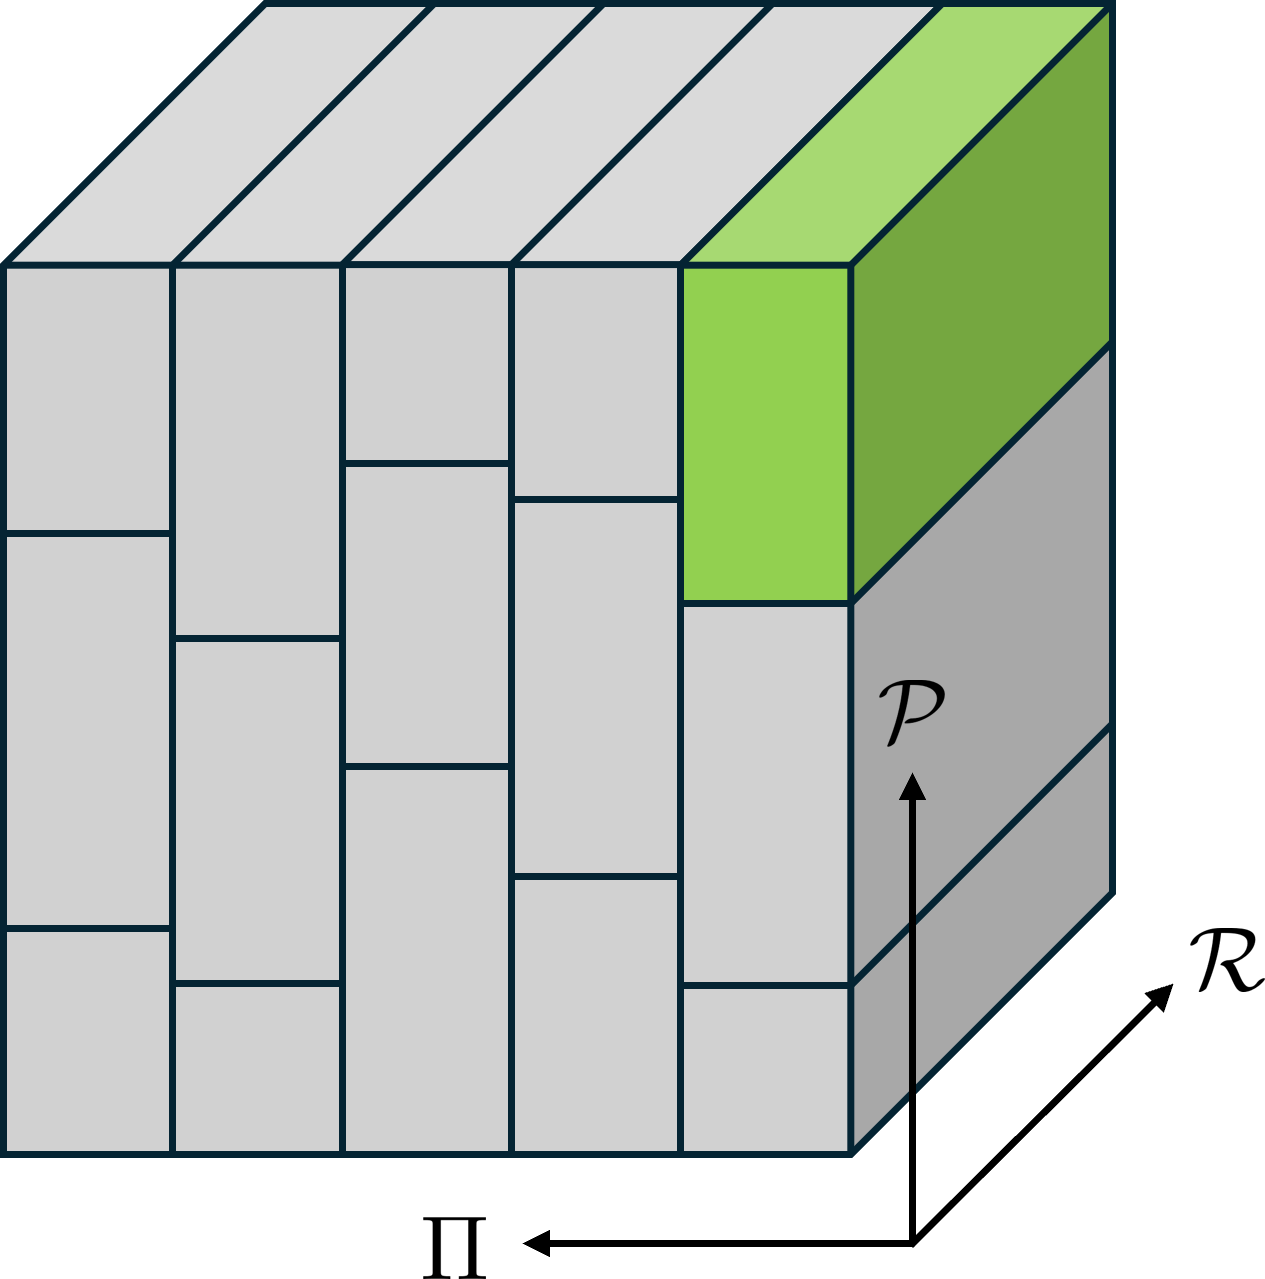
\includegraphics[width=0.3\textwidth]{Picture1.png}
\caption{Partitioning for hybrid MDPs}\label{fig: illustrate}
\end{figure}

\pref{fig: illustrate} illustrates the partition scheme over $\calM\times \Pi=\calP\times \calR\times \Pi$ described in \pref{assum: function approximation hybrid}. Each infoset $\phi$ (represented by the green block in \pref{fig: illustrate}) is associated with single policy $\pi_\phi$, a subset of transitions, and all reward functions. %Under a fixed policy $\pi$, transition $P$ and transition $P'$ should lie in the same $\phi$ if $Q^{\pi}(s,a; (P, R)) = Q^{\pi}(s,a; (P', R))$ for all $s,a,R$. 
As shown in \pref{fig: illustrate}, the partition over the $\calP$ space could be different for different $\pi$. 


\subsection{Algorithm and regret decomposition}
%\begin{align*}
%    \hair_\eta^{\Phi, D, \hattP_\Phi}(p, \nu; \rho) &=\E_{\pi\sim p} \E_{(\phi, P, R)\sim \nu}\E_{o\sim M_{P,R}(\cdot|\pi)} \\
%    &\qquad \left[V_{\hattP_\phi, R}(\pi_\phi) - V_{P,R}(\pi) - \frac{1}{\eta}\KL\left(\nu_{\bo{\phi}}(\cdot|\pi, o), \rho\right) - \right]
%\end{align*}
\begin{algorithm}[H]
    \caption{Model-free learning for the hybrid setting with bandit feedback and bilinear structure}
    \label{alg:MFHB}
    \jz{We don't need any specific algorithms anymmore, correct?}
    %\textbf{Input:} %Partition set $\Phi =  \left\{\phi_{\pi, f}: \pi \in \Pi, f \in \calF^\pi\right\}$,  $\rho_1(\phi) = \frac{1}{|\Phi|},\, \forall \phi \in \Phi$, 
   %epoch length $\tau$, and learning rate $\eta, \beta, \gamma$. \\
   Let $\rho_1(\phi) = \frac{1}{|\Phi|}$ for all $\phi$. \\
   \For{\textup{\textbf{epoch}} $k=1, 2, \ldots, \frac{T}{\tau}$}{
      %Given $ D^\pi_{\hbi}(\phi, \hattP_\phi||P)$ defined in \pref{eq:h-bi-div} and $D^\pi(\nu\|\rho)$ in \pref{eq: our divergence}, 
      Let $p_{k}, \nu_k$ be the solution of the minimax optimization: 
        \begin{align*}
            &\min_{p \in \Delta(\Pi)}\max_{\nu \in \Delta(\Psi)} \air_\eta^{\Phi, D}(p, \nu; \rho_t).    %\E_{\pi \sim p}\E_{(M,\pi^\star) \sim \nu}\left[V_{M}(\pi^\star) -V_{M}(\pi) - \frac{1}{\eta}\E_{o \sim M(\pi)}\left[\KL\left(\nu_{\bo{\phi}}(\cdot|\pi, o), \rho_k\right)\right] - \frac{1}{\eta}\E_{\phi \sim \rho_k}\left[ D^\pi_{\hbi}(\phi||M)\right]\right].
            \numberthis \label{eq:minmax hybrid}
        \end{align*}
         Sample $\pi_k  \sim p_k$. \\
         \For{$i=1,\ldots, \tau$}{
        Execute $\pi_k$ and observes $o_{k,h}^i = (s_{k,h}^i, a_{k,h}^i, r_{k,h}^i, s_{k,h+1}^i)$ for all $h$.
         }        
         Define
        \begin{align}
        &L_k(\phi) = \max\limits_{R\in\calR}\sum_{h=1}^H \left(\frac{1}{\tau} \sum_{i \in [\tau]}\ellest_h(\phi, R; o_{k,h}^i)\right)^2,\label{eq:adv_Lk}
             \\&\rho_{k+1} = \argmin_{\rho\in \Delta(\Phi)}\left\{\inner{\rho, L_k} + \frac{1}{\beta \tau}\sum_{i=1}^\tau \KL(\rho, (\nu_k)_{\bo{\phi}}(\cdot|\pi_k, o_k^i)) + \frac{1}{\gamma}\KL(\rho, \rho_k) \right\}. \label{eq:rho-hybrid 2}
        \end{align}
        % where $o_k=(o^i_{k,h})_{h\in[H],i\in[\tau]}$ is all observations in epoch $k$. 
    %      Solve $\nu_k$ as 
    %      \begin{align*}
    %         \nu_k =  \E_{\pi\sim p_k} \E_{(M,\pi^\star)\sim \nu} \left[
    % V_{M}(\pi^\star) - V_{M}(\pi) - \frac{2}{\eta}\E_{o \sim M(\pi)}\left[\KL(\nu_{\phi|\pi, o}, \, \rho_k)\right]- \frac{1}{\eta} \E_{\phi \sim \rho_k}\left[L^\pi(\phi, P, R)\right] \right].
    %      \end{align*}
    %      Define $o_k = (o_k^1,\cdots, o_k^{\tau})$, and set 
    %     \begin{align*}
    %         \rho_{k+1}(\phi) = \nu_k(\phi|\pi_k, o_k)\exp\left(-L_k(\phi)\right) \quad \text{and} \quad L_k(\phi) = \max_{R}\sum_{h=1}^H \left(\frac{1}{\tau} \sum_{i \in [\tau]}\ellest_h(\phi, w_{k,h}^i, R)\right)^2
    %     \end{align*}
    }
\end{algorithm}

The choices of diverges in \pref{alg:MFHB}: 
\begin{align}
    &D^\pi(\nu\|\rho) = \E_{\phi\sim \rho}\E_{(P,R) \sim \nu}\E_{o \sim M_{P,R}(\cdot|\pi)}\left[\KL\left(\nu_{\bo{\phi}}(\cdot|\pi, o), \rho\right) + \E_{P_\phi\sim z(\cdot|\phi)}\left[\tilD^\pi(\phi\|P) \right]\right]  ,  \label{eq:adv_div}
    \\& \tilD^\pi(\phi\|P) = \tilD_{\hbi}^\pi(\phi\|P) = \max_{R}\sum_{h=1}^H\left(\E^{\pi, P}\left[\ellest_h\l(\phi, R; o_h)\right]\right)^2  \label{eq:adv_bi_div}
\end{align}
%with the definition of $\Phi$ following \pref{assum: function approximation hybrid}. For a fixed comparator policy $\pi^\star$, let $\phi^\star$ be the aggregation such that  $\pi_{\phi^\star} = \pi^\star$ and for any $((P,R), \pi^\star) \in \phi$, we have $Q^{\pi^\star}(s,a, (P, R')) = Q^{\pi^\star}(s,a, (P^\star, R'))$ for any $s,a, R'$. 
Note that although we defined $L_k(\phi)$ in \pref{eq:adv_Lk} with the full observations $o_{k,h}^i$, only the observations of transition is really used in $L_k(\phi)$ while the reward observation is discarded. This is because we would like $L_k(\phi)$ to capture only the value error due to the transition error \emph{under the worst choice of the reward function}. This is also why the definition of $L_k(\phi)$ involves a maximization over $R$. % Instead, to tackle the adversarial rewards, we take a $\max_{R}$ to consider the worst case reward in $L_k(\phi)$. 
%Correspondingly, we only use the transition information in $o_h$ in \pref{eq:adv_bi_div}, and the expectation $\E^{\pi, P}$ is only related to transitions. 

The regret is decomposed as the following. With abuse of notation, we use $\pi_t, \rho_t, \nu_t$ to denote $\pi_k, \rho_k, \nu_k$ if $t$ is in epoch $k$. 
\iffalse
\begin{align*}
    &V_{P^\star, R_t}(\pi_{\phi^\star}) - \E_{\pi\sim p_t} [V_{P^\star, R_t}(\pi)]\\
    &= \E_{\pi\sim p_t}\left[ V_{\hatP_{\phi^\star}, R_t}(\pi_{\phi^\star}) - V_{P^\star, R_t}(\pi) - \frac{1}{\eta} D^{\pi}(\delta_{P^\star, R_t} \| \rho_t; \hatP_\Phi) \right]  + \frac{1}{\eta}  \E_{\pi\sim p_t} \left[D^\pi(\delta_{P^\star, R_t} \| \rho_t; \hatP_\Phi)\right] \\
    &\qquad \qquad + \left( V_{P^\star, R_t}(\pi_{\phi^\star}) - V_{\hatP_{\phi^\star}, R_t}(\pi_{\phi^\star})\right)   \\
    &\leq \max_{z} \E_{\pi\sim p_t}\left[ \E_{P_{\phi^\star}\sim z(\cdot|\phi^\star) } \left[V_{P_{\phi^\star}, R_t}(\pi_{\phi^\star})\right] - V_{P^\star, R_t}(\pi) - \frac{1}{\eta} D^{\pi}(\delta_{P^\star, R_t} \| \rho_t; z) \right]   + \frac{1}{\eta}   \E_{\pi\sim p_t} \left[D^\pi(\delta_{P^\star, R_t} \| \rho_t; \hatP_\Phi)\right] \\
    &\leq \max_\nu \max_{z} \E_{\pi\sim p_t}\E_{(\phi, P, R)\sim \nu}\left[ \E_{P_\phi\sim z(\cdot|\phi)} \left[V_{P_{\phi}, R}(\pi_{\phi})\right] - V_{P, R}(\pi) - \frac{1}{\eta} D^{\pi}(\nu \| \rho_t; z) \right]  \\
    &\qquad \qquad - \E_{\pi\sim p_t} \left[\breg_{D^{\pi}}\right] \\
    &\qquad \qquad + \frac{1}{\eta} \sum_{t=1}^T  \E_{\pi\sim p_t} \left[D^\pi(\delta_{P^\star, R_t} \| \rho_t; \hatP_\Phi)\right] \\
    %&\qquad \qquad + \underbrace{\frac{1}{\eta} \sum_h \E_{\phi\sim \rho} \left(\E^{\pi_t, P^\star}[\ellest_h(\phi, P_{\phi, t}, R_t; o_h)]\right)^2}_{\text{handle this separately}}
\end{align*}
\fi

\begin{align}
&\Reg(\pi_{\phi^\star}) \nonumber
%\\&= \E[\Reg(\pi^\star)] \nonumber
    \\&=\sum_{t=1}^T \left(V_{M_t}(\pi_{\phi^\star}) - \E_{\pi\sim p_t}[V_{M_t}(\pi)]\right)  \nonumber
    \\&\le   \sum_{t=1}^T \underbrace{\min_{p \in \Delta(\Pi)}\max_{\nu \in \Delta(\calM \times \Pi)}\air^{\Phi, D}_\eta(p,\nu; \rho_t)}_{\textbf{Complexity}} + \frac{1}{\eta} \underbrace{\sum_{t=1}^T \E_{\pi\sim p_t}\left[D^{\pi}(\delta_{M_t,\pi^\star}\|\rho_t) - \breg_{D^{\pi}(\cdot\|\rho_t)}(\delta_{M_t,\pi^\star}, \nu_t)\right] }_{\est}. \label{eq:adv_bi_init_decom 2}
\end{align}




% $\left(X(\phi')^\top\E_{R \sim \nu(\cdot|\phi)}\left[\theta(R)\right] - X(\phi')^\top\E_{R \sim \nu}\left[\theta(R)\right]\right)$

% \subsection{Bounding the estimation error}


% Since every $M_t = (P^\star, R_t)$ shares the same transition $P^\star$, every $(M_t, \pi^\star)$ lies in $\phi^\star$. From the definition of divergence in \pref{eq:adv_div} and \pref{eq:adv_bi_div},  as we divide the $T$ rounds into $K$ epoch, we have
% \begin{align}
%     &\est\nonumber
%     \\&=   \sum_{t=1}^T \left(D^{\pi_t}(\delta_{M_t,\pi^\star}\|\rho_t) - \breg_{D^{\pi_t}(\cdot\|\rho_t)}(\delta_{M_t,\pi^\star}, \nu_t)\right) \nonumber
%     \\&=  \sum_{t=1}^T \Bigg(\log\left(\frac{1}{\rho_t(\phi^\star)}\right) +  \E_{\pi \sim p_t}\E_{\phi\sim \rho_t}\left[\sum_{h=1}^H\left(\E^{\pi, P^\star}\left[\ellest_h(\phi; o_h, R_t)\right]\right)^2  \right] \nonumber \\
%     &\qquad \qquad \qquad \qquad - \E_{\pi \sim p_t}\E_{o \sim M_t(\cdot|\pi)}\left[\KL\left(\delta_{\phi^\star}, (\nu_t)_{\bo{\phi}}(\cdot|\pi, o)\right) \right]\Bigg)\nonumber
%     \\&= \sum_{t=1}^T \E_{\pi \sim p_t}\E_{o \sim M_t(\cdot|\pi)}\left[\log\left(\frac{\nu_t(\phi^\star|\pi, o)}{\rho_t(\phi^\star)}\right)\right] +  \sum_{t=1}^T\E_{\pi \sim p_t}\E_{\phi\sim \rho_t}\left[D_{\bi}^{\pi}(\phi||P^\star, R_t)\right] \nonumber
%     \\&\le \sum_{k=1}^K \E_{\pi \sim p_k}\left[\sum_{i=1}^\tau \E_{o \sim M_{(k-1)\tau + i}(\cdot|\pi)}\left[\log\left(\frac{\nu_k(\phi^\star|\pi, o)}{\rho_k(\phi^\star)}\right)\right]\right] \nonumber \\
%     &\qquad \qquad \qquad \qquad + \sum_{k=1}^K\sum_{i=1}^{2\tau}\E_{\pi \sim p_k}\E_{\phi\sim \rho_k}\left[\max_{R \in \mathcal{R}}D_{\bi}^{\pi}(\phi||P^\star, R)\right]\label{eq:est_adv_fir 2}
% \end{align}
% % With sum of KL in the update of $\rho_{k+1}$, we have a term
% % \begin{align*}
% %     \frac{1}{\eta} \sum_{k=1}^K\sum_{i=1}^\tau\log\left(\frac{\rho_{k}(\phi^\star)}{\nu_k(\phi^\star|\pi_k,o_k^i)}\right) 
% % \end{align*}
% where the second equality uses the fact that
% \begin{align*}
%     \breg_{D^{\pi}(\cdot\|\rho_t)}(\nu, \nu') = \E_{M \sim \nu}\E_{o \sim M(\cdot|\pi)}\left[\KL\left(\nu_{\bo{\phi}}(\cdot|\pi, o), \nu_{\bo{\phi}}'(\cdot|\pi, o)\right)\right].
% \end{align*}

% Applying \pref{lem: online esitmation epoch general} with
% \begin{align*}
%     \ellest_h(\phi, R; o^i_{k,h}) &= f_{\phi}(s^i_{k,h}, a^i_{k,h}; R) - R(s^i_{k,h}, a^i_{k,h}) - f_\phi(s^i_{k,h+1}; R) \\
%     \ell^j_{k,h}(\phi) &= \ellest_h(\phi, R^j; o^i_{k,h}), \qquad \text{where} \ \ R^j(s,a) = \varphi(s,a)^\top \mathbf{e}_j \\
%     F_k^i(\rho) &= \KL(\rho, (\nu_k)_{\bo{\phi}} (\cdot|\pi_k, o^i_k) )
% \end{align*}
% % \jz{ Do we still need to bound the estimation error separately here?}
% % \jz{I mean using the theorem 7}
% % \HL{I think we can directly use the lemma 33 you wrote for $\sum_{k=1}^K\sum_{i=1}^{2\tau}\E_{\pi \sim p_k}\E_{\phi\sim \rho_k}\left[\max_{R \in \mathcal{R}}D_{\bi}^{\pi}(\phi||P^\star, R)\right]$, then}
% % \HL{It seems we can use theorem 7 everywhere? Actually where is the proof for theorem 7. For hybrid bilinear $N = d$?}
% % \jz{Theorem 7 is for non bc and theorem 8 for bc}\jz{Yes. the proof is in appendix H}
% % \HL{Cool I will delete the redundant proof}

% We have
% \begin{align*}
%         % &\sum_{k=1}^K\sum_{i=1}^{2\tau}\E_{\phi \sim \rho_k}\left[\left(\E^{P^\star, \pi_k}\left[\ell_h(\phi;o_{k,h}^i)\right]\right)^2\right] 
%         &\sum_{k=1}^K\sum_{i=1}^{2\tau}\E_{\pi \sim p_k}\E_{\phi\sim \rho_k}\left[\max_{R \in \mathcal{R}}D_{\bi}^{\pi}(\phi||P^\star, R)\right]
%         \\ &\le \frac{\log|\Phi|}{\gamma} +  \sum_{k=1}^K \left(\sum_{i=1}^{2\tau}(  F_k^i(\delta_{\phi^\star}) - F_k^i(\rho_{k+1}) - \breg_{F_k^i}(\delta_{\phi^\star}, \rho_{k+1}) \right) + 90B^2HT^{\frac{1}{3}}N^\frac{2}{3}
%         \\&=  \sum_{k=1}^K \sum_{i=1}^{2\tau} \log\left(\frac{\rho_{k+1}(\phi^\star)}{\nu_k(\phi^\star|\pi_k,o_k^i)}\right) - \sum_{k=1}^K\sum_{i=1}^{2\tau}\KL(\rho_{k+1}, (\nu_k)_{\bo{\phi}} (\cdot|\pi_k, o^i_k) ) + 90B^2HT^{\frac{1}{3}}N^\frac{2}{3}
%         \\&\le  \sum_{k=1}^K \sum_{i=1}^{2\tau} \log\left(\frac{\rho_{k}(\phi^\star)}{\nu_k(\phi^\star|\pi_k,o_k^i)}\right) + \sum_{k=1}^K \sum_{i=1}^{2\tau} \log\left(\frac{\rho_{k+1}(\phi^\star)}{\rho_k(\phi^\star)}\right) + 90B^2HT^{\frac{1}{3}}\log|\Phi|N^\frac{2}{3} +  \frac{\log|\Phi|}{\gamma}
% \end{align*}
% Thus, we have
% \begin{align*}
%     &\E\left[\est\right]
%     \\&\le \sum_{k=1}^K \E_{\pi \sim p_k}\left[\sum_{i=1}^\tau \E_{o \sim M_{(k-1)\tau + i}(\cdot|\pi)}\left[\log\left(\frac{\nu_k(\phi^\star|\pi, o)}{\rho_k(\phi^\star)}\right)\right]\right] \nonumber \\
%     &\qquad \qquad \qquad \qquad + \sum_{k=1}^K\sum_{i=1}^{2\tau}\E_{\pi \sim p_k}\E_{\phi\sim \rho_k}\left[\max_{R \in \mathcal{R}}D_{\bi}^{\pi}(\phi||P^\star, R)\right]
% \end{align*}



% Old bound
% \begin{align*}
%     &\frac{1}{8}\sum_{k=1}^K\E_{\pi \sim p_k}\E_{\phi \sim \rho_k}\left[\max_{R \in \calR} D_{\hbi}^{\pi}(\phi\|P^\star, R)\right] 
%     \\&\le  \frac{1}{\beta}\sum_{k=1}^K\sum_{i=1}^\tau\log\left(\frac{\rho_{k+1}(\phi^\star)}{\nu_k(\phi^\star|\pi_k,o_k^i)}\right) + \frac{1}{\gamma}\sum_{k=1}^K\log\left(\frac{\rho_{k+1}(\phi^\star)}{\rho_k(\phi^\star)}\right) + 3HK\epsilon_{\conc}^2 + 4HL^2\log(|\Phi|/\delta)
%     \\&\leq \frac{1}{\beta}\sum_{k=1}^K\sum_{i=1}^\tau\log\left(\frac{\rho_{k}(\phi^\star)}{\nu_k(\phi^\star|\pi_k,o_k^i)}\right) + \left(\frac{1}{\gamma} + \frac{\tau}{\beta}\right)\log|\Phi| + \frac{6HK\log\left(KH|\Phi||\calR|/\delta\right)}{\tau}+ 4HL^2\log(|\Phi|/\delta). 
% \end{align*}





% \cw{Remove the rest of the proof for $\est$ and use the result in \pref{app: batching improve} with 
% \begin{align*}
%     \ellest_h(\phi, R; o^i_{k,h}) &= f_{\phi}(s^i_{k,h}, a^i_{k,h}; R) - R(s^i_{k,h}, a^i_{k,h}) - f_\phi(s^i_{k,h+1}; R) \\
%     \ell^j_{k,h}(\phi) &= \ellest_h(\phi, R^j; o^i_{k,h}), \qquad \text{where} \ \ R^j(s,a) = \varphi(s,a)^\top \mathbf{e}_j \\
%     F_k^i(\rho) &= \KL(\rho, (\nu_k)_{\bo{\phi}} (\cdot|\pi_k, o^i_k) )
% \end{align*}


% }

% Now we show that the estimation error can be well-bounded. Recall the update rule of $\rho_{k+1}$ (\pref{eq:rho-hybrid 2}): 
% \begin{align*}
%     \rho_{k+1} = \argmin_{\rho\in \Delta(\Phi)}\left\{ 
% \inner{\rho, L_k} + \frac{1}{\beta}\sum_{i=1}^\tau\KL(\rho, (\nu_k)_{\bo{\phi}}(\cdot|\pi_k, o_k^i) + \frac{1}{\gamma}\KL(\rho, \rho_k) \right\}. 
% \end{align*}
% where $L_k(\phi) =\max_R \sum_{h=1}^H\big(\frac{1}{\tau}\sum_{i=1}^{\tau} \ellest_h(\phi; o_{k,h}^i, R)\big)^2$. From \pref{lem: bregman}, we have
% \begin{align*}
%     &\inner{\rho_{k+1}, L_k} + \frac{1}{\beta}\sum_{i=1}^\tau\KL(\rho_{k+1}, (\nu_k)_{\bo{\phi}}(\cdot|\pi_k, o_k^i)) + \frac{1}{\gamma} \KL(\rho_{k+1}, \rho_k)
%     \\&\le \inner{\delta_{\phi^\star}, L_k} + \frac{1}{\beta}\sum_{i=1}^\tau\KL(\delta_{\phi^\star}, (\nu_k)_{\bo{\phi}}(\cdot|\pi_k, o_k^i)) + \frac{1}{\gamma} \KL(\delta_{\phi^\star}, \rho_k) \\
%     &\qquad \qquad \qquad \qquad -  \frac{1}{\beta}\sum_{i=1}^\tau\KL\left(\delta_{\phi^\star}, \rho_{k+1} \right) - \frac{1}{\gamma} \KL\left(\delta_{\phi^\star}, \rho_{k+1} \right)
% \end{align*}
% Thus, by setting $\gamma = \frac{1}{2HL^2}$, we have $0 \le \gamma L_k \le \frac{1}{2}$ and
% \begin{align*}
%     &\inner{\rho_{k}, L_k} 
%     \\&\le \inner{\rho_k - \rho_{k+1}, L_k} -  \frac{1}{\gamma}\KL(\rho_{k+1}, \rho_k) + L_k(\phi^\star) + \frac{1}{\beta}\sum_{i=1}^\tau\log\left(\frac{\rho_{k+1}(\phi^\star)}{\nu_k(\phi^\star|\pi_k,o_k^i)}\right) + \frac{1}{\gamma}\log\left(\frac{\rho_{k+1}(\phi^\star)}{\rho_k(\phi^\star)}\right) 
%     \\&\le \gamma \inner{\rho_k, L_k^2} + L_k(\phi^\star) + \frac{1}{\beta}\sum_{i=1}^\tau\log\left(\frac{\rho_{k+1}(\phi^\star)}{\nu_k(\phi^\star|\pi_k,o_k^i)}\right) + \frac{1}{\gamma}\log\left(\frac{\rho_{k+1}(\phi^\star)}{\rho_k(\phi^\star)}\right) \tag{\pref{lem:stability}}
%     \\&\le \frac{1}{2}\cdot\inner{\rho_k, L_k} + L_k(\phi^\star) + \frac{1}{\beta}\sum_{i=1}^\tau\log\left(\frac{\rho_{k+1}(\phi^\star)}{\nu_k(\phi^\star|\pi_k,o_k^i)}\right) + \frac{1}{\gamma}\log\left(\frac{\rho_{k+1}(\phi^\star)}{\rho_k(\phi^\star)}\right). 
% \end{align*}
% This implies
% \begin{align}
%     \frac{1}{2}\E_{\phi \sim \rho_k}\left[L_k(\phi)\right] \le L_k(\phi^\star) + \frac{1}{\beta}\sum_{i=1}^\tau\log\left(\frac{\rho_{k+1}(\phi^\star)}{\nu_k(\phi^\star|\pi_k,o_k^i)}\right) + \frac{1}{\gamma}\log\left(\frac{\rho_{k+1}(\phi^\star)}{\rho_k(\phi^\star)}\right)  \label{eq:rho_no_conc_adv}
% \end{align}
% By Hoeffding's inequality and union bound, with probability at least $1-\delta$, for any $k\in[K]$, $h\in[H]$, and any $\phi \in \Phi, R \in \calR$, we have
% \begin{align*}
% \left|\frac{1}{\tau} \sum_{i \in [\tau]}\ellest_h(\phi; o_{k,h}^i, R) -  \E^{ \pi_k,\, P^\star}\left[\ellest_h(\phi; o_h, R)\right]\right| \le \sqrt{\frac{2\log\left(KH|\Phi||\calR|/\delta\right)}{\tau}} = \epsilon_{\conc}. 
% \end{align*}
% Recall $D_{\hbi}^\pi(\phi\|P^\star, R) = \sum_{h=1}^H  \left(\E^{\pi, P^\star}\left[\ellest_h(\phi, o_h, R)\right]\right)^2$. The concentration inequality together with the inequality $(u+v)^2\leq 2u^2 + 2v^2$ imply for every $\phi\in\Phi$ and $R\in\calR$ and $k\in[K]$,%and define $L_k(\phi, R) = \sum_{h=1}^H \left(\frac{1}{\tau} \sum_{i \in [\tau]}\ellest_h(\phi, o_{k,h}^i, R)\right)^2$, we have 
% \begin{align*}
%     &\sum_{h=1}^H \left(\frac{1}{\tau} \sum_{i \in [\tau]}\ellest_h(\phi, o_{k,h}^i, R)\right)^2 \le 2 D_{\hbi}^{\pi_k}(\phi\|P^\star, R)  + 2H\epsilon_{\conc}^2,
%      \\&\sum_{h=1}^H \left(\frac{1}{\tau} \sum_{i \in [\tau]}\ellest_h(\phi, o_{k,h}^i, R)\right)^2 \ge \frac{1}{2}D_{\hbi}^{\pi_k}(\phi\|P^\star, R)  -H\epsilon_{\conc}^2. 
% \end{align*}
% % From Lemma A.3 in \cite{foster2021statistical}, with probability at least $1-\delta$, for any $\phi \in \Phi$, we have
% % \begin{align*}
% %    \frac{1}{2}\sum_{k=1}^K \E_{\pi \sim p_k}\left[L^\pi(\phi, P^\star, R)\right] \le   \sum_{k=1}^K D_{bi}^{\pi_k}(\phi||P^\star, R_k) + 4H\log(|\Phi|/\delta). 
% % \end{align*}
% These imply 
% \begin{align}
%     L_k(\phi)&=\max_{R\in\calR}\sum_{h=1}^H \left(\frac{1}{\tau} \sum_{i \in [\tau]}\ellest_h(\phi, o_{k,h}^i, R)\right)^2 \le 2 \max_{R\in\calR} D_{\hbi}^{\pi_k}(\phi\|P^\star, R)  + 2H\epsilon_{\conc}^2,\label{eq:adv_conc1}
%      \\L_k(\phi)&=\max_{R\in\calR}\sum_{h=1}^H \left(\frac{1}{\tau} \sum_{i \in [\tau]}\ellest_h(\phi, o_{k,h}^i, R)\right)^2 \ge \frac{1}{2}\max_{R\in\calR} D_{\hbi}^{\pi_k}(\phi\|P^\star, R)  -H\epsilon_{\conc}^2. \label{eq:adv_conc2}
% \end{align}


% %Thus, let $R_0 =  \argmax_{R \in \calR} L_k(\phi, R)$ and $R_1 = \argmax_{R \in \calR} D_{\hbi}^{\pi_k}(\phi\|P^\star, R)$, for any $\phi \in \Phi$, since $L_k(\phi) = L_k(\phi, R_0)$, we have
% %\begin{align}
% %&L_k(\phi) - 2\max_{R \in \calR} D_{\hbi}^{\pi_k}(\phi\|P^\star, R) = L_k(\phi, R_0) - 2D_{\hbi}^{\pi_k}(\phi\|P^\star, R_0) + \underbrace{2D_{\hbi}^{\pi_k}(\phi\|P^\star, R_0) - 2D_{\hbi}^{\pi_k}(\phi\|P^\star, R_1)}_{\le 0} \le 2H\epsilon_{conc}^2 \label{eq:adv_conc1}
% %\\&\frac{1}{2}\max_{R \in \calR} D_{\hbi}^{\pi_k}(\phi\|P^\star, R) - L_k(\phi) = \frac{1}{2}D_{\hbi}^{\pi_k}(\phi\|P^\star, R_1) - L_k(\phi, R_1) + \underbrace{L_k(\phi, R_1) - L_k(\phi, R_0)}_{\le 0} \le H\epsilon_{conc}^2 \label{eq:adv_conc2}
% %\end{align}
% From Lemma A.3 in \cite{foster2021statistical}, with probability at least $1-\delta$, for any $\phi \in \Phi$, we have
% \begin{align}
%    \frac{1}{2}\sum_{k=1}^K \E_{\pi \sim p_k}\left[\max_{R \in \calR} D_{\hbi}^{\pi}(\phi||P^\star, R)\right] \le   \sum_{k=1}^K \max_{R \in \calR} D_{\hbi}^{\pi_k}(\phi||P^\star, R) + 4HL^2\log(|\Phi|/\delta).  \label{eq:adv_policy_conc}
% \end{align}

% Combining \pref{eq:rho_no_conc_adv}, \pref{eq:adv_conc1}, \pref{eq:adv_conc2}, \pref{eq:adv_policy_conc}, using the fact that $D_{\hbi}^{\pi}(\phi^\star||P^\star, R) = 0$ for every $\pi$, and summing over $k$, we have
% with probability at least $1-2\delta$,  \begin{align*}
%     &\frac{1}{8}\sum_{k=1}^K\E_{\pi \sim p_k}\E_{\phi \sim \rho_k}\left[\max_{R \in \calR} D_{\hbi}^{\pi}(\phi\|P^\star, R)\right] 
%     \\&\le  \frac{1}{\beta}\sum_{k=1}^K\sum_{i=1}^\tau\log\left(\frac{\rho_{k+1}(\phi^\star)}{\nu_k(\phi^\star|\pi_k,o_k^i)}\right) + \frac{1}{\gamma}\sum_{k=1}^K\log\left(\frac{\rho_{k+1}(\phi^\star)}{\rho_k(\phi^\star)}\right) + 3HK\epsilon_{\conc}^2 + 4HL^2\log(|\Phi|/\delta)
%     \\&\leq \frac{1}{\beta}\sum_{k=1}^K\sum_{i=1}^\tau\log\left(\frac{\rho_{k}(\phi^\star)}{\nu_k(\phi^\star|\pi_k,o_k^i)}\right) + \left(\frac{1}{\gamma} + \frac{\tau}{\beta}\right)\log|\Phi| + \frac{6HK\log\left(KH|\Phi||\calR|/\delta\right)}{\tau}+ 4HL^2\log(|\Phi|/\delta). 
% \end{align*}
% Putting this back to \pref{eq:est_adv_fir 2} and choose $\beta = 8\tau$, we have
% \begin{align*}
%     &\est\nonumber
%     \\&\le  \sum_{k=1}^K \E_{\pi \sim p_k}\left[\sum_{i=1}^\tau \E_{o \sim M_{(k-1)\tau + i}(\cdot|\pi)}\left[\log\left(\frac{\nu_k(\phi^\star|\pi, o)}{\rho_k(\phi^\star)}\right)\right]\right] +  \tau \sum_{k=1}^K\E_{\pi \sim p_k}\E_{\phi\sim \rho_k}\left[\max_{R \in \mathcal{R}}D_{\bi}^{\pi}(\phi||P^\star, R)\right] 
%     \\&\le \sum_{k=1}^K \E_{\pi \sim p_k}\left[\sum_{i=1}^\tau \E_{o \sim M_{(k-1)\tau + i}(\cdot|\pi)}\left[\log\left(\frac{\nu_k(\phi^\star|\pi, o)}{\rho_k(\phi^\star)}\right)\right]\right] +  \sum_{k=1}^K\sum_{i=1}^\tau\log\left(\frac{\rho_{k}(\phi^\star)}{\nu_k(\phi^\star|\pi_k,o_k^i)}\right)
%     \\& \qquad \qquad + \otil\left( \frac{HT\log(|\Phi||\calR|/\delta)}{\tau } + \tau HL^2\log(|\Phi|/\delta)\right). 
% \end{align*}
% where $\otil$ here only omits $\log(HT)$.
% Thus, taking expectation and use $K = \frac{T}{\tau}$, we have
% \begin{align*}
%     \E\left[\est\right] \le  \otil\left( \frac{HT\log(|\Phi||\calR|)}{\tau } + \tau HL^2\log(|\Phi|)\right) = \otil\left( HL\log|\Phi|\sqrt{T\log|\calR|} \right) 
% \end{align*}
% where we choose the optimal $\tau=\frac{\sqrt{T\log|\calR|}}{L}$. 



% % Now we move to bound the \textbf{complexity} term in \pref{eq:stoc_bi_init_decom}. From \pref{lem:adv_complexity}, we have
% % \begin{align*}
% %     \textbf{complexity} &\le T\cdot\mfdec_\eta^{\tilD,\Phi}
% %     \\&\le T\cdot\odec_\eta^{\tilD,\Phi}  + \eta T
% % \end{align*} \HL{Need prove this for adv settings}
% % Given the definition of $\tilD$ in \pref{eq:stoc_bi_div}, from Lemma 20 in \cite{liu2025decision}. 
% % \begin{itemize}
% %     \item If for every $\phi \in \Phi$, $\esttt(\pi_{\phi}) = \pi_{\phi}$, then $\odec_\eta^{\tilD,\Phi}  \le \order(dH\eta)$.
% %     \item If there exists $\phi \in \Phi$ such that $\esttt(\pi_{\phi}) \neq \pi_{\phi}$, then $\odec_\eta^{\tilD,\Phi}  \le \order(H\sqrt{d\eta})$ if $\eta \le \frac{1}{dH^2}$.
% % \end{itemize}



\subsection{Proof of \pref{thm: bilinear-adv}}
From \pref{thm: avg est}, with $N = d$, we have
\begin{align*}
    \E\left[\est\right] \le HB^2d^{\frac{2}{3}}T^{\frac{1}{3}}\log\left(|\Phi|\right)
\end{align*}
Combine with the complexity bound in \pref{lem: digdec_adv < d hbi}, we have the following results:

Thus, if for every $\phi \in \Phi$, $\esttt(\pi_{\phi}) = \pi_{\phi}$, and $B \le 1$,  we can bound the regret as 
\begin{align*}
    \E[\Reg(\pi_{\phi^\star})] \leq \otil\left(\eta^{\frac{1}{3}}d^{\frac{1}{3}}H^{\frac{2}{3}}\cdot T + \frac{ Hd^{\frac{2}{3}}T^{\frac{1}{3}}\log\left(|\Phi|\right)}{\eta}\right)
\end{align*}
which is $\otil\left(H^{\frac{3}{4}}d^{\frac{5}{12}}T^{\frac{5}{6}}\log(|\Phi|)^{\frac{1}{4}}\right)$
by choosing $\eta = H^{\frac{1}{4}}d^{\frac{1}{4}}T^{-\frac{1}{2}}\log(|\Phi|)^{\frac{3}{4}}$. %, $\tau = \sqrt{T}$, we have regret $\otil\left(\sqrt{dH^2L^2\log(|\Phi||\calR|)}T^{\frac{3}{4}}\right)$.


% \begin{itemize}
%     \item If $\esttt(\pi_{\phi}) = \pi_{\phi}$ for all $\phi$, then $\alpha = 0$, and $\max_\nu \qcom^{\Phi, \tilD_\hbi}_\eta(\nu) \le \order\left(\eta^{\frac{1}{3}}d^{\frac{1}{3}}H^{\frac{2}{3}}\right)$
%     \item  If there exists a $\phi$ such that  $\esttt(\pi_\phi) \neq \pi_{\phi}$, then setting $\alpha = 3H\sqrt{\eta d}$, we have $\max_\nu \qcom^{\Phi, \tilD_\hbi}_\eta(\nu) \le \order\left(\eta^{\frac{1}{6}}d^{\frac{1}{6}}H^{\frac{1}{3}}\right)$. 
% \end{itemize}

Otherwise, if there exists a $\phi$ such that $\esttt(\pi_{\phi}) \neq \pi_{\phi}$, then $B \le |\calA|$ , the regret bound is 
\begin{align*}
    \E[\Reg(\pi_{\phi^\star})] \leq \otil\left(\eta^{\frac{1}{6}}d^{\frac{1}{6}}H^{\frac{1}{3}}\cdot T  + \frac{ H|\calA|^2d^{\frac{2}{3}}T^{\frac{1}{3}}\log\left(|\Phi|\right)}{\eta}\right)
\end{align*}
which is $\otil\left(H^{\frac{4}{7}}d^{\frac{5}{21}}T^{\frac{19}{21}}|\calA|^{\frac{2}{7}}\log|\Phi|^{\frac{1}{7}}\right)$ by choosing $\eta = H^{\frac{4}{7}}d^{\frac{3}{7}}T^{-\frac{4}{7}}|\calA|^{\frac{12}{7}}\log(|\Phi|)$. 

\fi
\newpage
\section{Omitted Details in \pref{sec: compare DEC}}\label{app:compare DEC}


\subsection{Proof of \pref{thm:lower bound}}
In this section, we will use $\text{Ber}(p)$ to denote Bernoulli distribution with success probability $p$. We consider parameters $\epsilon$ and $\Delta$ with $\epsilon < \Delta = \frac{1}{16\sqrt{T}} \leq \frac{1}{16}$. Define $p^+ = \frac{1}{2} + \Delta$ and $p^- = \frac{1}{2} - \Delta$. Let $\mathbb{H}(\nu)$ denote the entropy of distribution $\nu$. We assume learning rate $\eta \leq 1$.  

Consider a three-arm bandit environment with model class $\mathcal{M} = \{M_1, M_2\}$ where
\begin{itemize}
    \item $M_1 = \left(\text{Ber}\left(p^-\right), \text{Ber}\left(p^+\right), \epsilon\text{Ber}(0.5)\right)$. The reward distribution is $\text{Ber}\left(p^-\right)$ for arm $a_1$ and   $\text{Ber}\left(p^+\right)$ for arm $a_2$. Arm $a_3$'s reward is $0$ and $\epsilon$ with equal probability. 
    \item $M_2 = \left(\text{Ber}\left(p^+\right), \text{Ber}\left(p^-\right), 0.5\epsilon\right)$. The reward distribution is $\text{Ber}\left(p^+\right)$ for arm $a_1$ and  $\text{Ber}\left(p^-\right)$ for arm $a_2$. Arm $a_3$'s reward is $0.5\epsilon$ deterministically. 
\end{itemize}
In this setting, $\Phi$ contains two infosets (based on \pref{assum: function approximation stochastic}): 
\begin{align*}
    \phi_1 = \left\{\left(M_1, \pi_{M_1}\right)\right\},\quad \phi_2=\left\{\left(M_2, \pi_{M_2}\right)\right\}. 
\end{align*}
%We denote the two infoset as $\phi_1$ and $\phi_2$. 
In the rest of this proof, we compare the optimistic E2D algorithm \citep{foster2024model} and our algorithm in this environment. 

\paragraph{Optimistic DEC algorithm \citep{foster2024model}}
Given $\rho_t \in \Delta(\Phi)$, the algorithm chooses action distribution via
\begin{align}
    p_t = \argmin_{p \in \Delta(\Pi)} \max_{\nu \in \Delta(\Psi)} \E_{a\sim p} \E_{\phi\sim \rho_t} \E_{M\sim \nu} \left\{V_{\phi}(a_{\phi}) - V_M(a) - \frac{1}{\eta} D^{a}(\phi \| M) \right\}
\label{eq:dec-three}
\end{align}
where $a_{\phi}$ is the optimal action of infoset $\phi$. In this simple bandit setting, the bilinear divergence and the squared Bellman error coincide with
\begin{align*} 
 D^a(\phi\| M) = \left(\E^{a, M} [V_\phi(a) - r]\right)^2 = (V_\phi(a) - V_M(a))^2. 
\end{align*}
We first consider the divergence term, for action $a \in \{a_1, a_2\}$, we have
\begin{align}
    \E_{\phi \sim \rho_t}\E_{M \sim \nu}\left[D^a(\phi \| M)\right] &= \rho_t(\phi_1)\nu(M_2)(V_{\phi_1}(a) - V_{M_2}(a))^2 +  \rho_t(\phi_2)\nu(M_1)(V_{\phi_2}(a) - V_{M_1}(a))^2 \nonumber
    \\&= 4\left(\rho_t(\phi_1)\nu(M_2) + \rho_t(\phi_2)\nu(M_1)\right)\Delta^2 \label{eq:D12}
\end{align}
For action $a = a_3$, we have
\begin{align}
    \E_{\phi \sim \rho_t}\E_{M \sim \nu}\left[D^a(\phi\| M)\right] &= \rho_t(\phi_1)\nu(M_2)(V_{\phi_1}(a) - V_{M_2}(a))^2 +  \rho_t(\phi_2)\nu(M_1)(V_{\phi_2}(a) - V_{M_1}(a))^2 \nonumber
    \\&= 0 
    \label{eq:D3}
\end{align}
Thus, for any $\rho_t$ and $\nu$, we have
\begin{align*}
\E_{a \sim p}\E_{\phi\sim \rho_t} \E_{M\sim \nu}\left[ - \frac{1}{\eta} D^{a}(\phi\|M)\right]  &= -\frac{4(1-p(a_3))\Delta^2}{\eta}\left(\rho_t(\phi_1)\nu(M_2) + \rho_t(\phi_2)\nu(M_1)\right) 
%\\&= -\frac{1}{\eta}\left(\rho_t(\phi_1)\nu(M_2) + \rho_t(\phi_2)\nu(M_1)\right)\left(4\Delta^2  + p(a_3)(\epsilon^2 - 4\Delta^2)\right),
\end{align*}
which is monotonically increasing in $p(a_3)$. 

We then consider the regret term. For any $p \in \Delta\left(\Pi\right)$, define $\Tilde{p} = \left(\frac{p(a_1)}{1-p(a_3)}, \frac{p(a_2)}{1-p(a_3)}, 0\right)$ if $p(a_3)<1$, and $\Tilde{p}=(\frac{1}{2}, \frac{1}{2}, 0)$ otherwise. For any $M \in \mathcal{M}$, when $p(a_3)<1$ we have 
\begin{align*}
    \E_{a \sim p}\left[V_{M}(a)\right] - \E_{a \sim \Tilde{p}}\left[V_M(a)\right] &=  \sum_{a \in \{a_1, a_2\}}\left(p(a) - \Tilde{p}(a)\right)V_{M}(a) + p(a_3)V_M(a_3) 
    \\&= \frac{-p(a_3)}{1-p(a_3)}\sum_{a \in \{a_1, a_2\}} p(a) V_M(a)  + p(a_3)V_M(a_3) 
    \\&\le \frac{-p(a_3)}{1-p(a_3)}\left(p(a_1) + p(a_2)\right)p^-  + p(a_3)V_M(a_3) \tag{$V_M(a) \ge p^-$ for any $M$ and $a \in \{a_1, a_2\}$, and $p(a_3) < 1$}
    \\&= p(a_3)\left(V_M(a_3) - \frac{1}{2} + \Delta\right)
    \\&\le p(a_3)\left(0.5\epsilon + \Delta -\frac{1}{2}\right) \le 0 \tag{$\epsilon < \Delta \leq \frac{1}{16}$}, 
\end{align*}
and when $p(a_3)=1$ we also have $\E_{a \sim p}\left[V_{M}(a)\right] - \E_{a \sim \Tilde{p}}\left[V_M(a)\right]\leq 0$.  
Thus, for any $\rho_t$, $\nu$, and $p$, 
\begin{align*}
    \E_{a\sim \Tilde{p}} \E_{\phi\sim \rho_t} \E_{M\sim \nu} \left\{V_\phi(a_\phi) - V_M (a)\right\} \le  \E_{a\sim p} \E_{\phi\sim \rho_t} \E_{M\sim \nu} \left\{V_\phi(a_\phi) - V_M(a)\right\}.
\end{align*}
Combining the discussion of the above two terms, for any $\rho_t, \nu$ and $p$, we have
\begin{align}
    \E_{a\sim \Tilde{p}} \E_{\phi\sim \rho_t} \E_{M\sim \nu} \left\{V_\phi(a_\phi) - V_M (a) - \frac{1}{\eta} D^{a}(\phi\|M) \right\} \le \E_{a\sim p} \E_{\phi\sim \rho_t} \E_{M\sim \nu} \left\{V_\phi(a_\phi) - V_M (a) - \frac{1}{\eta} D^{a}(\phi\| M) \right\}. 
\label{eq:minmax_start}
\end{align}
%Note that it is sufficient to consider $p$ with $p(a_3) < 1$ because $p(a_3) = 1$ is suboptimal.
% \begin{align*}
%     \E_{a\sim \delta_{a_2}} \E_{\phi\sim \rho_t} \E_{M\sim \nu} \left\{f_\phi(a_\phi) - f_M (a) - \frac{1}{\eta} D^{a}(\phi, M) \right\} \le \E_{a\sim \delta_{a_3}} \E_{\phi\sim \rho_t} \E_{M\sim \nu} \left\{f_\phi(a_\phi) - f_M (a) - \frac{1}{\eta} D^{a}(\phi, M) \right\} 
% \end{align*}
% where $\delta_{a_2}$ is the action distribution with $p(a_2) = 1$ and $\delta_{a_3}$ is the action distribution with $p(a_3) = 1$.


% Given that $f_{\phi}(a_{\phi}) = \frac{1}{2} + \Delta$ for both $\phi_1, \phi_2$, we have
% \begin{align*}
%     &\E_{a\sim p} \E_{\phi\sim \rho_t} \E_{M\sim \nu} \left\{f_\phi(a_\phi) - f_M (a)\right\}
%      \\&= p^+- \nu(M_1)p(a_1)f_{M_1}(a_1) - \nu(M_1)p(a_2)f_{M_1}(a_2) - \nu(M_1)p(a_3)f_{M_1}(a_3) 
%      \\& \qquad - \nu(M_2)p(a_1)f_{M_2}(a_1) - \nu(M_2)p(a_2)f_{M_2}(a_2) - \nu(M_2)p(a_3)f_{M_2}(a_3) 
%      \\&=  p^+- \nu(M_1)p(a_1)f_{M_1}(a_1) - \nu(M_1)p(a_2)f_{M_1}(a_2) - \nu(M_1)p(a_3)f_{M_1}(a_3) 
%      \\& \qquad - \nu(M_2)p(a_1)f_{M_2}(a_1) - \nu(M_2)p(a_2)f_{M_2}(a_2) - \nu(M_2)p(a_3)f_{M_2}(a_3) 
% \end{align*}


Given \pref{eq:minmax_start}, the minimax solution of \pref{eq:dec-three} must have $p_t(3) = 0$ for any $\rho_t$ and any $t$. This implies that the optimistic DEC algorithm will never choose $a_3$ and the problem degenerate to standard two-arm bandit, so the policy derived from optimistic DEC objective \pref{eq:dec-three} must suffer standard regret lower bound $\E\left[\Reg(\pi_{M^\star})\right] \ge \Omega(\sqrt{T})$ given $\Delta = \Theta\left(\frac{1}{\sqrt{T}}\right)$.

\paragraph{Our algorithm}
%\cw{Let $\rho_1$ be a uniform distribution. 

%If $a=a_3$, the learner can tell which environment it is in after seeing the observation, it holds that $\nu_{\bo{\phi}}(\cdot|a_3,o) = \delta_{\phi_1}$ or $\delta_{\phi_2}$. Therefore, 
%\begin{align*}
%    \E_{o\sim M(a_3)}\left[\KL(\nu_{\bo{\phi}}(\cdot|a_3,o) , \rho_1)\right] = \ln \frac{1}{1/2} = \ln 2. 
%\end{align*}
%On the other hand, if $a=a_1$ or $a=a_2$, 
%\begin{align*}
%    \E_{o\sim M(a)}\left[\KL(\nu_{\bo{\phi}}(\cdot|a,o) , \rho_1)\right] &=  \E_{o\sim M(a)}\left[\KL(\nu_{\bo{\phi}}(\cdot|a,o) , \nu_{\bo{\phi}})\right] + \KL(\nu_{\bo{\phi}}, \rho_1) \\
%    &= \E_{\phi\sim \nu}\left[\KL(\nu_{\bo{o}}(\cdot|a,\phi) , \nu_{\bo{o}}(\cdot|a))\right] + \KL(\nu_{\bo{\phi}}, \rho_1) \\
%    &\leq \KL\left(\text{Ber}(p^+, p^-)\right) + \KL(\nu_{\bo{\phi}}, \rho_1) \\
%    &\leq \Delta^2 + \KL(\nu_{\bo{\phi}}, \rho_1). 
%\end{align*}
%}



Given $\rho_1$ is a uniform distribution, we consider our first step optimization where
\begin{align}
    p_1 = \argmin_{p \in \Delta(\Pi)} \max_{\nu \in \Delta(\Psi)} \E_{a\sim p} \E_{\phi\sim \rho_1} \E_{M\sim \nu} \left\{V_M(a_M) - V_M (a) -\frac{1}{\eta} \E_{o\sim M(\cdot|a)}\left[\KL(\nu_{\bo{\phi}}(\cdot|a, o), \rho_1)\right] - \frac{1}{\eta} D^{a}(\phi\| M) \right\}. 
\label{eq:dec-our}
\end{align}
% where $\rho_1$ is a uniform distribution over $\Phi$.  For arm $a\in\{1,2,3\}$. Define
% \begin{align*}
%     J(a):=\max_{\nu \in \Delta(\Psi)} \E_{\phi\sim\rho_1}\E_{M\sim\nu}\left[
% f_\phi(a_\phi) - f_M(a) - \frac{1}{\eta} \E_{o\sim M(a)}\left[\KL(\nu_\phi(\cdot|a, o), \rho_1)\right] - \frac{1}{\eta}\,D^a(\phi,M)
% \right].
% \end{align*}
%
% Since $\rho_1$ is a uniform distribution, since observation $o \in \{0,1\}$, we have
%
% We have
% \begin{align*}
%     \nu(\phi_1|a_1, 1) &= \frac{\mathbb{P}(1|a_1, \phi_1)\mathbb{P}(a_1|\phi_1)\nu(\phi_1)}{\mathbb{P}(a_1)\sum_{\phi}\mathbb{P}(1|a_1, \phi)\nu(\phi)}
%     \\&= \frac{\mathbb{P}(1|a_1, \phi_1)\nu(\phi_1)}{\sum_{\phi}\mathbb{P}(1|a_1, \phi)\nu(\phi)} \tag{$\mathbb{P}(a_1|\phi) = \mathbb{P}(a_1)$}
%     \\&= \frac{\left(p^-\right)\nu(\phi_1)}{\left(p^-\right)\nu(\phi_1) + \left(\frac{1}{2} + \Delta\right)\nu(\phi_2)}
% \end{align*}
% Similarly, we have
% \begin{align*}
%     &\nu(\phi_2|a_1, 1) = \frac{\left(\frac{1}{2} + \Delta\right)\nu(\phi_2)}{\left(p^-\right)\nu(\phi_1) + \left(\frac{1}{2} + \Delta\right)\nu(\phi_2)}
%     \\&\nu(\phi_1|a_1, 0) = \frac{\left(\frac{1}{2} + \Delta\right)\nu(\phi_1)}{\left(\frac{1}{2} + \Delta\right)\nu(\phi_1) + \left(p^-\right)\nu(\phi_2)} \qquad \nu(\phi_2|a_1, 0) = \frac{\left(p^-\right)\nu(\phi_2)}{\left(\frac{1}{2} + \Delta\right)\nu(\phi_1) + \left(p^-\right)\nu(\phi_2)}
%     \\& \nu(\phi_1|a_2, 1) = \frac{\left(\frac{1}{2} + \Delta\right)\nu(\phi_1)}{\left(\frac{1}{2} + \Delta\right)\nu(\phi_1) + \left(p^-\right)\nu(\phi_2)}  \qquad   \nu(\phi_2|a_2, 1) = \frac{\left(p^-\right)\nu(\phi_2)}{\left(\frac{1}{2} + \Delta\right)\nu(\phi_1) + \left(p^-\right)\nu(\phi_2)}
%     \\& \nu(\phi_1|a_2, 0) = \frac{\left(p^-\right)\nu(\phi_1)}{\left(p^-\right)\nu(\phi_1) + \left(\frac{1}{2} + \Delta\right)\nu(\phi_2)}  \qquad   \nu(\phi_2|a_2, 0) = \frac{\left(\frac{1}{2} + \Delta\right)\nu(\phi_2)}{\left(p^-\right)\nu(\phi_1) + \left(\frac{1}{2} + \Delta\right)\nu(\phi_2)}
% \end{align*}
% For any binary distribution $(x, 1-x)$ where $0 \le x \le 1$, we have
% \begin{align*}
%     \KL\left(\left(x, 1-x\right), \left(\frac{1}{2}, \frac{1}{2}\right)\right) = x\ln\left(2x\right) + (1-x)\ln\left(2(1-x)\right) = \ln\left(2\right) - H(x)
% \end{align*}
% where $H(x)$ is the entropy of distribution $(x, 1-x)$. Thus,
%
%
% \begin{align*}
% &\E_{o\sim M_1(a_1)}\left[\KL(\nu_\phi(\cdot|a_1, o), \rho_1)\right] = \left(p^-\right)\left(\ln(2) - H(\nu_\phi(\cdot|a_1, 1))\right) + \left(\frac{1}{2} +\Delta\right)\left(\ln(2) - H(\nu_\phi(\cdot|a_1, 0))\right)
% \\&\E_{o\sim M_2(a_1)}\left[\KL(\nu_\phi(\cdot|a_1, o), \rho_1)\right] = \left(\frac{1}{2} + \Delta\right)\left(\ln(2) - H(\nu_\phi(\cdot|a_1, 1))\right) + \left(\frac{1}{2} -\Delta\right)\left(\ln(2) - H(\nu_\phi(\cdot|a_1, 0))\right)
% \\&\E_{o\sim M_1(a_2)}\left[\KL(\nu_\phi(\cdot|a_2, o), \rho_1)\right] = \left(\frac{1}{2} + \Delta\right)\left(\ln(2) - H(\nu_\phi(\cdot|a_2, 1))\right) + \left(p^-\right)\left(\ln(2) - H(\nu_\phi(\cdot|a_2, 0))\right)
% \\&\E_{o\sim M_2(a_2)}\left[\KL(\nu_\phi(\cdot|a_2, o), \rho_1)\right] = \left(p^-\right)\left(\ln(2) - H(\nu_\phi(\cdot|a_2, 1))\right) + \left(\frac{1}{2} +\Delta\right)\left(\ln(2) - H(\nu_\phi(\cdot|a_2, 0))\right)
% \\&\E_{o\sim M_1(a_3)}\left[\KL(\nu_\phi(\cdot|a_3, o), \rho_1)\right] =  \KL(\nu_\phi(\cdot|a_3, 0), \rho_1) = \ln(2) - H(\nu_\phi(\cdot|a_3, 0)) = \ln(2)
% \\&\E_{o\sim M_2(a_3)}\left[\KL(\nu_\phi(\cdot|a_3, o), \rho_1)\right] =  \KL(\nu_\phi(\cdot|a_3, \epsilon), \rho_1)  =  \ln(2) - H(\nu_\phi(\cdot|a_3, \epsilon)) = \ln(2)
% \end{align*}
% where the last two equalities comes from the deterministic reward of $a_3$ in both environments.
%%
%
% We also have
% \begin{align*}
%     \KL\left(\right)
% \end{align*}
%
Below, we discuss the four terms in \pref{eq:dec-our}. \\

\noindent\underline{The $V_M(a_M)$ term}\ \ \ For any $\nu$, we have $\E_{M\sim \nu}[V_M(a_M)] = p^+$, which is a constant. Therefore, this term can be ignored in the objective. \\


\noindent\underline{The $V_M(a)$ term}\ \ \ 
By direct calculation, we have 
\begin{align}
    &\E_{a\sim p} \E_{M\sim \nu} \left[V_M (a) \right]= \frac{p(a_1) + p(a_2)}{2} + \left(p(a_1) - p(a_2)\right)\left(\nu(M_2) - \nu(M_1)\right)\Delta + 0.5p(a_3)\epsilon. \label{eq: temp 111} 
\end{align}
For any $p = (p(a_1), p(a_2), p(a_3))$, consider $\hat{p} = (\frac{p(a_1) + p(a_2)}{2}, \frac{p(a_1) + p(a_2)}{2}, p(a_3))$. By \pref{eq: temp 111} we have
\begin{align}
    \max_{\nu \in \Delta(\Psi)}\E_{a\sim \hat{p}} \E_{M\sim \nu} \left[-V_M (a)\right] \leq \max_{\nu \in \Delta(\Psi)}\E_{a\sim p} \E_{M\sim \nu} \left[-V_M (a)\right]. 
\label{eq:modify_p}
\end{align}

\noindent\underline{The $D^a(\phi\|M)$ term} \ \ \ Given $\rho_1$ is a uniform distribution, for action $a \in \{1,2\}$, from \pref{eq:D12}, for any $\nu$  we have $\E_{\phi \sim \rho_1}\E_{M \sim \nu}\left[D^a(\phi\|M)\right] = 2\Delta^2$. For action $a = 3$, from \pref{eq:D3}, for any $\nu$,  we have $\E_{\phi \sim \rho_1}\E_{M \sim \nu}\left[D^a(\phi\|M)\right] = 0$. Hence, $\E_{a\sim p}\E_{\phi \sim \rho_1}\E_{M \sim \nu}\left[D^a(\phi\|M)\right] = 2(1-p(a_3))\Delta^2$.  Note that now this is independent of  $\nu$, and only related to $p(a_3)$ or $p(a_1) + p(a_2)$ but not $p(a_1)$ or $p(a_2)$ individually. \\



\noindent\underline{The $\KL$ term}\ \ \ Notice that 
\begin{align*}
    &\nu_{\bo{o}}(\cdot|a_1, \phi_1) = \text{Ber}\left(p^-\right),  \quad  \nu_{\bo{o}}(\cdot|a_2, \phi_1) = \text{Ber}\left(p^+\right), \quad \nu_{\bo{o}}(\cdot|a_1, \phi_2) = \text{Ber}\left(p^+\right),  \quad \nu_{\bo{o}}(\cdot|a_2, \phi_2) = \text{Ber}\left(p^-\right),
    \\&\nu_{\bo{o}}(\cdot|a_1) =\text{Ber}\left(m_1\right),  \qquad \nu_{\bo{o}}(\cdot|a_2) =\text{Ber}\left(m_2\right),
\end{align*}
where $m_1 = \nu(\phi_1)p^- +  \nu(\phi_2)p^+$ and $m_2 =\nu(\phi_1)p^+ +  \nu(\phi_2)p^-$ and it holds that $m_1 + m_2 = 1$.  Given that $\KL\left(\text{Ber}\left(p\right), \text{Ber}\left(q\right)\right) = \KL\left(\text{Ber}\left(1-p\right), \text{Ber}\left(1-q\right)\right)$, we have
\begin{align*}
&\E_{a\sim p} \E_{M\sim \nu} \left[\E_{o\sim M(a)}\left[\KL(\nu_{\pmb{\phi}}(\cdot|a, o), \rho_1)\right]\right]
\\&= \E_{a\sim p} \E_{\phi \sim \nu}\left[\KL(\nu_{\pmb{o}}(\cdot|a, \phi), \nu_{\pmb{o}}(\cdot|a))\right]+ \KL(\nu_{\pmb{\phi}}, \rho_1)
\\&= p(a_1)\nu(\phi_1)\KL\left(\text{Ber}\left(p^-\right),  \text{Ber}\left(m_1\right)\right) +  p(a_2)\nu(\phi_1)\KL\left(\text{Ber}\left(p^+\right),  \text{Ber}\left(m_2\right)\right) + \KL(\nu_{\pmb{\phi}}, \rho_1)
    \\&\qquad + p(a_1)\nu(\phi_2)\KL\left(\text{Ber}\left(p^+\right),  \text{Ber}\left(m_1\right)\right) +  p(a_2)\nu(\phi_2)\KL\left(\text{Ber}\left(p^-\right),  \text{Ber}\left(m_2\right)\right) 
    \\&\qquad + p(a_3)\E_{\phi \sim \nu}\left[\KL(\nu_{\pmb{o}}(\cdot|a_3, \phi), \nu_{\pmb{o}}(\cdot|a_3))\right]
    \\&=  \left(p(a_1) + p(a_2)\right)\left(\nu(\phi_1)\KL\left(\text{Ber}\left(p^-\right),  \text{Ber}\left(m_1\right)\right) + \nu(\phi_2)\KL\left(\text{Ber}\left(p^+\right),  \text{Ber}\left(m_1\right)\right)\right)
    \\&\qquad + p(a_3)\mathbb{H}(\nu) + \KL(\nu_{\pmb{\phi}}, \rho_1)
    \\&= \left(1-p(a_3)\right)\left(\mathbb{H}\left(\text{Ber}(m_1)\right) - \mathbb{H}\left(\text{Ber}\left(p^+\right)\right)\right) + p(a_3)\mathbb{H}(\nu) +  \KL(\nu_{\pmb{\phi}}, \rho_1). 
\end{align*}

% \begin{align*}
%     &\E_{a\sim p} \E_{\phi \sim \nu}\left[\KL(\nu_{o}(\cdot|a, \phi), \nu_{o}(\cdot|a))\right]
%     \\&= p(a_1)\nu(\phi_1)\KL\left(\text{Ber}\left(p^-\right),  \text{Ber}\left(m_1\right)\right) +  p(a_2)\nu(\phi_1)\KL\left(\text{Ber}\left(p^+\right),  \text{Ber}\left(m_2\right)\right)
%     \\&\quad + p(a_1)\nu(\phi_2)\KL\left(\text{Ber}\left(p^+\right),  \text{Ber}\left(m_1\right)\right) +  p(a_2)\nu(\phi_2)\KL\left(\text{Ber}\left(p^-\right),  \text{Ber}\left(m_2\right)\right) 
%     \\&\qquad + p(a_3)\E_{\phi \sim \nu}\left[\KL(\nu_{o}(\cdot|a_3, \phi), \nu_{o}(\cdot|a_3))\right]
%     \\&= p(a_1)\nu(\phi_1)\KL\left(\text{Ber}\left(p^-\right),  \text{Ber}\left(m_1\right)\right) +  p(a_2)\nu(\phi_1)\KL\left(\text{Ber}\left(p^-\right),  \text{Ber}\left(m_1\right)\right)
%     \\&\quad + p(a_1)\nu(\phi_2)\KL\left(\text{Ber}\left(p^+\right),  \text{Ber}\left(m_1\right)\right) +  p(a_2)\nu(\phi_2)\KL\left(\text{Ber}\left(\frac{1}{2} + \Delta\right),  \text{Ber}\left(m_1\right)\right)
%      \\&\qquad + p(a_3)\left(\nu(\phi_1)\log\left(\frac{1}{\nu(\phi_1)}\right) + \nu(\phi_2)\log\left(\frac{1}{\nu(\phi_2)}\right)\right)
%     \\&= \left(p(a_1) + p(a_2)\right)\left(\nu(\phi_1)\KL\left(\text{Ber}\left(p^-\right),  \text{Ber}\left(m_1\right)\right) + \nu(\phi_2)\KL\left(\text{Ber}\left(\frac{1}{2} + \Delta\right),  \text{Ber}\left(m_1\right)\right)\right) + p(a_3)H(\nu)
%     \\&=  \left(p(a_1) + p(a_2)\right)\left(\nu(\phi_1)\left(\left(p^-\right)\log\left(\frac{p^-}{m_1}\right) + \left(\frac{1}{2} + \Delta\right)\log\left(\frac{\frac{1}{2} + \Delta}{1-m_1}\right) \right) + \right. 
%     \\&\qquad \left. \nu(\phi_2)\left(\left(\frac{1}{2} + \Delta\right)\log\left(\frac{\frac{1}{2} + \Delta}{m_1}\right) + \left(p^-\right)\log\left(\frac{\frac{1}{2} -\Delta}{1-m_1}\right) \right) \right) + p(a_3)H(\nu)
%     \\&= \left(p(a_1) + p(a_2)\right)\left(H\left(\text{Ber}(m_1)\right) - H\left(\text{Ber}\left(\frac{1}{2} + \Delta\right)\right)\right) + p(a_3)H(\nu)
% \end{align*}
% Thus
% \begin{align*}
%     &\min_{\nu}\E_{a\sim p} \E_{M\sim \nu} \left[\E_{o\sim M(a)}\left[\KL(\nu_\phi(\cdot|a, o), \rho_1)\right]\right]
%     \\&= \left(1-p(a_3)\right)\left(H\left(\text{Ber}(m_1)\right) - H\left(\text{Ber}\left(\frac{1}{2} + \Delta\right)\right)\right) + \KL\left(\nu_{\phi}, \rho_1\right) + p(a_3)H(\nu)
% \end{align*}


Note that this term is only related to $p(a_3)$ or $p(a_1)+p(a_2)$, but not $p(a_1)$ or $p(a_2)$ individually. \\

\noindent\underline{Combining terms} \ \ \ 
Combining the case discussions above, for any $p = (p(a_1), p(a_2), p(a_3))$, with $\hat{p} = (\frac{p(a_1) + p(a_2)}{2}, \frac{p(a_1) + p(a_2)}{2}, p(a_3))$, we have
\begin{align*}
    &\max_{\nu \in \Delta(\Psi)}\left\{\E_{a\sim \hat{p}} \E_{M\sim \nu} \left[-V_M (a) - \frac{1}{\eta}\E_{o\sim M(a)}\left[\KL(\nu_{\pmb{\phi}}(\cdot|a, o), \rho_1)\right]-\frac{1}{\eta}\E_{\phi\sim \rho_1}[D^a(\phi\|M)]\right]\right\}  
    \\&\le \max_{\nu \in \Delta(\Psi)}\left\{\E_{a\sim p} \E_{M\sim \nu} \left[-V_M (a)- \frac{1}{\eta}\E_{o\sim M(a)}\left[\KL(\nu_{\pmb{\phi}}(\cdot|a, o), \rho_1)\right]-\frac{1}{\eta}\E_{\phi\sim \rho_1}[D^a(\phi\|M)]\right]\right\}. 
\end{align*}
To calculate the max value of the left-hand-side,  consider policy distribution $p_s = (\frac{1-s}{2}, \frac{1-s}{2}, s)$. We have
\begin{align}
    &\E_{a\sim p_s} \E_{M\sim \nu} \left[-V_M (a) - \frac{1}{\eta}\E_{o\sim M(a)}\left[\KL(\nu_{\pmb{\phi}}(\cdot|a, o), \rho_1)\right]-\frac{1}{\eta}\E_{\phi\sim \rho_1}[D^a(\phi\|M)]\right] \nonumber
    \\&= \frac{s-1}{2}-\frac{s\epsilon}{2} -\frac{1}{\eta}\left( \left(1-s\right)\left(\mathbb{H}\left(\text{Ber}(m_1)\right) - \mathbb{H}\left(\text{Ber}(p^+)\right) + 2\Delta^2\right) +  \KL\left(\nu_{\pmb{\phi}}, \rho_1\right) + s\mathbb{H}(\nu) \right) \label{eq: G_init}
\end{align}
where $m_1 = \nu(\phi_1)p^{-} +  \nu(\phi_2)p^{+}$. Define
\begin{align*}
    G(\nu) = (1-s)\mathbb{H}(\text{Ber}(m_1)) + \KL\left(\nu_{\pmb{\phi}}, \rho_1\right) + s\mathbb{H}(\nu). 
\end{align*}


To calculate $\max_{\nu}$ of \pref{eq: G_init}, we only need to consider $ \min_{\nu}\left\{G(\nu)\right\}$. By setting $\nu(\phi_2) = 1 - \nu(\phi_1)$,  function $G$ is only related to $\nu(\phi_1)$ and we denote it as $G(\nu(\phi_1))$, after taking derivative, we have
\begin{align*}
    G'(\nu(\phi_1))&=(1-s)\ln\left(\frac{1-m_1}{m_1}\right)\left(p^{-} - p^+\right) + \log\left(\frac{\nu(\phi_1)}{1-\nu(\phi_1)}\right) + s\log\left(\frac{1-\nu(\phi_1)}{\nu(\phi_1)}\right)
    \\&= -\Delta(1-s)\ln\left(\frac{1-m_1}{m_1}\right) + \log\left(\frac{\nu(\phi_1)}{1-\nu(\phi_1)}\right) + s\log\left(\frac{1-\nu(\phi_1)}{\nu(\phi_1)}\right)
\end{align*}
where $m_1 = \nu(\phi_1)p^{-} +  (1- \nu(\phi_1))p^{+}$ and we use the fact that $\frac{\mathrm{d}\mathbb{H}(\text{Ber}(p))}{\mathrm{d}p} = \ln\left(\frac{1-p}{p}\right)$. Note that when $\nu(\phi_1) = \frac{1}{2}$ we have $m_1 = \frac{1}{2}$ and $G'(\frac{1}{2}) = 0$. Thus, $\frac{1}{2}$ is a stationary point. On the other hand, we have $G''(\frac{1}{2}) = 4(1-s - 2(1-s)\Delta^2) \geq 0$ and $G(\nu(\phi_1)) = G(1- \nu(\phi_1))$. This implies $\nu(\phi_1) = \frac{1}{2}$ is the unique minimizer and the minimal value is $G(\frac{1}{2}) = \ln(2)$.

Thus, 
\begin{align*}
  &\max_{\nu \in \Delta(\Psi)}\left\{\E_{a\sim p_s} \E_{M\sim \nu} \left[-V_M (a) - \frac{1}{\eta}\E_{o\sim M(a)}\left[\KL(\nu_{\pmb{\phi}}(\cdot|a, o), \rho_1)\right]-\frac{1}{\eta}\E_{\phi\sim \rho_1}[D^a(\phi\|M)]\right]\right\} \\
  &= \frac{s-1}{2} - \frac{s\epsilon}{2} -\frac{1}{\eta} \left(1-s\right) \left(-\mathbb{H}\left(\text{Ber}(p^+)\right) + 2\Delta^2\right) - \frac{1}{\eta}  \ln(2)
  \\&= (1-s) \left(-\frac{1-\epsilon}{2} + \frac{\mathbb{H}(\text{Ber}(p^+)) - 2\Delta^2}{\eta}\right) - \frac{\ln 2}{\eta} -\frac{\epsilon}{2}.   \numberthis \label{eq: tmp334}
\end{align*}
%Thus, the maximum value of the whole objective is %$\cw{the last term you added to the objective also involve $\nu$ --- why can you add this part after you already find the maximizer $\nu$ for the previous part?  }
%\begin{align*}
%    &\max_{\nu \in \Delta(\Psi)}\left\{\E_{a\sim p_s}\E_{\phi \sim \rho_1}\E_{M\sim \nu} \left[V_{M}(a_{M}) - V_M (a) - \frac{1}{\eta}\E_{o\sim M(a)}\left[\KL(\nu_{\pmb{\phi}}(\cdot|a, o), \rho_1)\right] -\frac{1}{\eta}D^a(\phi, M)\right]\right\}  
%    \\&=  p^++ \frac{s-1}{2} -\frac{1}{\eta} \left(s-1\right) \mathbb{H}\left(\text{Ber}\left(p^+\right)\right) - \frac{1}{\eta}  \ln(2) - \frac{2(1-s)\Delta^2}{\eta} - \frac{s\epsilon^2}{2\eta}
%\end{align*}
Note that 
\begin{align*}
    &\mathbb{H}(\text{Ber}(p^+)) - 2\Delta^2 \\
    &= -\KL(\text{Ber}(p^+), \text{Ber}(\tfrac{1}{2})) + \ln 2 - 2D_{\textrm{TV}}^2(\text{Ber}(p^+), \text{Ber}(\tfrac{1}{2})) 
    \\&\geq \ln 2 - 5\KL(\text{Ber}(p^+), \text{Ber}(\tfrac{1}{2}))  \tag{Pinsker's inequality}
    \\&\geq \ln 2 - 15\Delta^2  \tag{$\KL(\text{Ber}(\frac{1}{2}+\Delta), \text{Ber}(\frac{1}{2}))\leq 3\Delta^2$ for $\Delta\leq \frac{1}{2}$}
    \\&\geq \frac{1}{2}.   \tag{by the assumption $\Delta = \frac{1}{16\sqrt{T}}\leq \frac{1}{16}$}
\end{align*}

Hence, the minimum value of \pref{eq: tmp334} is achieved at $s=1$ when $\frac{1}{2\eta} - \frac{1-\epsilon}{2}\geq 0$.  By the condition $\eta\leq 1$, this indeed holds. This means that 
%When $s = 1$, this equation is equal to $   - \frac{1}{\eta}  \ln(2) $, and when $s = 0$, the equation is equal to $ \Delta + \frac{1}{\eta}\mathbb{H}\left(\text{Ber}\left(p^+\right)\right) - \frac{1}{\eta}  \ln(2) - \frac{2\Delta^2}{\eta} $. Given that $\eta   <   2\mathbb{H}\left(\text{Ber}\left(p^+\right)\right)  - 4\Delta^2 + \epsilon^2$, the minimal value is achieved when $s = 1$, which means 
our algorithm always picks the third arm in the first round. After picking arm $a_3$, the belief of $\phi$ will be deterministic, since $\nu_1(\phi|a_3, o)=0$ for any $\phi\neq \phi^\star$. 
%and $\nu_1(\phi|a_3, o)$ is deterministic on the ground-truth environment, 
This means the algorithm will always choose the optimal action in the following rounds, ensuring that $\E\left[\Reg(\pi_{M^\star})\right] \leq p^+ < 1$.





% Write $m_1 = \nu(\phi_1)p^{-} +  (1-\nu(\phi_1))p^{+}$, take gradient of above equation, we get
% \begin{align*}
%     (1-s)\ln\left(\frac{1-m_1}{m_1}\right)\left(p^{-} - p^+\right)
% \end{align*}


% For any $p$, we have $\frac{dH(\text{Ber}(p))}{dp} = \ln\left(\frac{1-p}{p}\right)$




% Then $p_1(a_3) = 1$ and afterwards the model will always choose the optimal action based on the update rule of $\rho$, which ensures $\max_{M \in \calM}\E\left[\Reg(M)\right] = 1$.


\end{document}